\documentclass[twoside]{book}

% Packages required by doxygen
\usepackage{fixltx2e}
\usepackage{calc}
\usepackage{doxygen}
\usepackage[export]{adjustbox} % also loads graphicx
\usepackage{graphicx}
\usepackage[utf8]{inputenc}
\usepackage{makeidx}
\usepackage{multicol}
\usepackage{multirow}
\PassOptionsToPackage{warn}{textcomp}
\usepackage{textcomp}
\usepackage[nointegrals]{wasysym}
\usepackage[table]{xcolor}

% Font selection
\usepackage[T1]{fontenc}
\usepackage[scaled=.90]{helvet}
\usepackage{courier}
\usepackage{amssymb}
\usepackage{sectsty}
\renewcommand{\familydefault}{\sfdefault}
\allsectionsfont{%
  \fontseries{bc}\selectfont%
  \color{darkgray}%
}
\renewcommand{\DoxyLabelFont}{%
  \fontseries{bc}\selectfont%
  \color{darkgray}%
}
\newcommand{\+}{\discretionary{\mbox{\scriptsize$\hookleftarrow$}}{}{}}

% Page & text layout
\usepackage{geometry}
\geometry{%
  a4paper,%
  top=2.5cm,%
  bottom=2.5cm,%
  left=2.5cm,%
  right=2.5cm%
}
\tolerance=750
\hfuzz=15pt
\hbadness=750
\setlength{\emergencystretch}{15pt}
\setlength{\parindent}{0cm}
\setlength{\parskip}{3ex plus 2ex minus 2ex}
\makeatletter
\renewcommand{\paragraph}{%
  \@startsection{paragraph}{4}{0ex}{-1.0ex}{1.0ex}{%
    \normalfont\normalsize\bfseries\SS@parafont%
  }%
}
\renewcommand{\subparagraph}{%
  \@startsection{subparagraph}{5}{0ex}{-1.0ex}{1.0ex}{%
    \normalfont\normalsize\bfseries\SS@subparafont%
  }%
}
\makeatother

% Headers & footers
\usepackage{fancyhdr}
\pagestyle{fancyplain}
\fancyhead[LE]{\fancyplain{}{\bfseries\thepage}}
\fancyhead[CE]{\fancyplain{}{}}
\fancyhead[RE]{\fancyplain{}{\bfseries\leftmark}}
\fancyhead[LO]{\fancyplain{}{\bfseries\rightmark}}
\fancyhead[CO]{\fancyplain{}{}}
\fancyhead[RO]{\fancyplain{}{\bfseries\thepage}}
\fancyfoot[LE]{\fancyplain{}{}}
\fancyfoot[CE]{\fancyplain{}{}}
\fancyfoot[RE]{\fancyplain{}{\bfseries\scriptsize Generated by Doxygen }}
\fancyfoot[LO]{\fancyplain{}{\bfseries\scriptsize Generated by Doxygen }}
\fancyfoot[CO]{\fancyplain{}{}}
\fancyfoot[RO]{\fancyplain{}{}}
\renewcommand{\footrulewidth}{0.4pt}
\renewcommand{\chaptermark}[1]{%
  \markboth{#1}{}%
}
\renewcommand{\sectionmark}[1]{%
  \markright{\thesection\ #1}%
}

% Indices & bibliography
\usepackage{natbib}
\usepackage[titles]{tocloft}
\setcounter{tocdepth}{3}
\setcounter{secnumdepth}{5}
\makeindex

% Hyperlinks (required, but should be loaded last)
\usepackage{ifpdf}
\ifpdf
  \usepackage[pdftex,pagebackref=true]{hyperref}
\else
  \usepackage[ps2pdf,pagebackref=true]{hyperref}
\fi
\hypersetup{%
  colorlinks=true,%
  linkcolor=blue,%
  citecolor=blue,%
  unicode%
}

% Custom commands
\newcommand{\clearemptydoublepage}{%
  \newpage{\pagestyle{empty}\cleardoublepage}%
}

\usepackage{caption}
\captionsetup{labelsep=space,justification=centering,font={bf},singlelinecheck=off,skip=4pt,position=top}

%===== C O N T E N T S =====

\begin{document}

% Titlepage & ToC
\hypersetup{pageanchor=false,
             bookmarksnumbered=true,
             pdfencoding=unicode
            }
\pagenumbering{roman}
\begin{titlepage}
\vspace*{7cm}
\begin{center}%
{\Large Gateware Libraries }\\
\vspace*{1cm}
{\large Generated by Doxygen 1.8.11}\\
\end{center}
\end{titlepage}
\clearemptydoublepage
\tableofcontents
\clearemptydoublepage
\pagenumbering{arabic}
\hypersetup{pageanchor=true}

%--- Begin generated contents ---
\chapter{Gateware Libraries}
\label{index}\hypertarget{index}{}\begin{DoxyCopyright}{Copyright}
Copyright (c) 2016 7th\+Gate Software .L\+LC 
\end{DoxyCopyright}
\begin{DoxyParagraph}{License\+:}
Gateware libraries are released under Creative Commons M\+IT lincense unless noted differently by the library. 
\end{DoxyParagraph}
\begin{DoxyVersion}{Version}
Beta Release
\end{DoxyVersion}
\hypertarget{index_API}{}\section{A\+P\+I\+Overview}\label{index_API}
Coming Soon\hypertarget{index_APIOverview}{}\subsection{G\+Log}\label{index_APIOverview}
Coming Soon\hypertarget{index_GLog}{}\subsection{G\+File}\label{index_GLog}
Coming Soon\hypertarget{index_GFile}{}\subsection{G\+Input}\label{index_GFile}
Coming Soon\hypertarget{index_GInput}{}\subsection{G\+Buffered\+Input}\label{index_GInput}
Coming Soon\hypertarget{index_Installation}{}\section{Installation}\label{index_Installation}
Coming Soon\hypertarget{index_Bug}{}\section{Reporting}\label{index_Bug}
Coming Soon 
\chapter{L\+I\+C\+E\+N\+SE}
\label{md_LICENSE}
\hypertarget{md_LICENSE}{}
The M\+IT License (M\+IT)

Copyright (c) 2016 7th\+Gate Software .L\+LC

Permission is hereby granted, free of charge, to any person obtaining a copy of this software and associated documentation files (the \char`\"{}\+Software\char`\"{}), to deal in the Software without restriction, including without limitation the rights to use, copy, modify, merge, publish, distribute, sublicense, and/or sell copies of the Software, and to permit persons to whom the Software is furnished to do so, subject to the following conditions\+:

The above copyright notice and this permission notice shall be included in all copies or substantial portions of the Software.

T\+HE S\+O\+F\+T\+W\+A\+RE IS P\+R\+O\+V\+I\+D\+ED \char`\"{}\+A\+S I\+S\char`\"{}, W\+I\+T\+H\+O\+UT W\+A\+R\+R\+A\+N\+TY OF A\+NY K\+I\+ND, E\+X\+P\+R\+E\+SS OR I\+M\+P\+L\+I\+ED, I\+N\+C\+L\+U\+D\+I\+NG B\+UT N\+OT L\+I\+M\+I\+T\+ED TO T\+HE W\+A\+R\+R\+A\+N\+T\+I\+ES OF M\+E\+R\+C\+H\+A\+N\+T\+A\+B\+I\+L\+I\+TY, F\+I\+T\+N\+E\+SS F\+OR A P\+A\+R\+T\+I\+C\+U\+L\+AR P\+U\+R\+P\+O\+SE A\+ND N\+O\+N\+I\+N\+F\+R\+I\+N\+G\+E\+M\+E\+NT. IN NO E\+V\+E\+NT S\+H\+A\+LL T\+HE A\+U\+T\+H\+O\+RS OR C\+O\+P\+Y\+R\+I\+G\+HT H\+O\+L\+D\+E\+RS BE L\+I\+A\+B\+LE F\+OR A\+NY C\+L\+A\+IM, D\+A\+M\+A\+G\+ES OR O\+T\+H\+ER L\+I\+A\+B\+I\+L\+I\+TY, W\+H\+E\+T\+H\+ER IN AN A\+C\+T\+I\+ON OF C\+O\+N\+T\+R\+A\+CT, T\+O\+RT OR O\+T\+H\+E\+R\+W\+I\+SE, A\+R\+I\+S\+I\+NG F\+R\+OM, O\+UT OF OR IN C\+O\+N\+N\+E\+C\+T\+I\+ON W\+I\+TH T\+HE S\+O\+F\+T\+W\+A\+RE OR T\+HE U\+SE OR O\+T\+H\+ER D\+E\+A\+L\+I\+N\+GS IN T\+HE S\+O\+F\+T\+W\+A\+RE. 
\chapter{R\+E\+A\+D\+ME}
\label{md_README}
\hypertarget{md_README}{}
Gateware Libraries

This is currently Beta released code. This code is subject to Interface Changes and bugs.

Please report any bugs with this build to underdog specifing the revision number. Revision number\# 78f9e2 
\chapter{Namespace Index}
\section{Namespace List}
Here is a list of all documented namespaces with brief descriptions\+:\begin{DoxyCompactList}
\item\contentsline{section}{\mbox{\hyperlink{namespace_g_w}{GW}} \\*The core namespace to which all Gateware interfaces/structures/defines must belong }{\pageref{namespace_g_w}}{}
\item\contentsline{section}{\mbox{\hyperlink{namespace_g_w_1_1_a_u_d_i_o}{G\+W\+::\+A\+U\+D\+IO}} \\*The namespace to which all Gateware library interfaces must belong }{\pageref{namespace_g_w_1_1_a_u_d_i_o}}{}
\item\contentsline{section}{\mbox{\hyperlink{namespace_g_w_1_1_c_o_r_e}{G\+W\+::\+C\+O\+RE}} \\*The core namespace to which all Gateware fundamental interfaces must belong }{\pageref{namespace_g_w_1_1_c_o_r_e}}{}
\item\contentsline{section}{\mbox{\hyperlink{namespace_g_w_1_1_g_r_a_p_h_i_c_s}{G\+W\+::\+G\+R\+A\+P\+H\+I\+CS}} \\*The namespace to which all Gateware Graphics library interfaces must belong }{\pageref{namespace_g_w_1_1_g_r_a_p_h_i_c_s}}{}
\item\contentsline{section}{\mbox{\hyperlink{namespace_g_w_1_1_m_a_t_h}{G\+W\+::\+M\+A\+TH}} \\*The namespace to which all math library interface must belong }{\pageref{namespace_g_w_1_1_m_a_t_h}}{}
\item\contentsline{section}{\mbox{\hyperlink{namespace_g_w_1_1_s_y_s_t_e_m}{G\+W\+::\+S\+Y\+S\+T\+EM}} \\*The namespace to which all Gateware library interfaces must belong }{\pageref{namespace_g_w_1_1_s_y_s_t_e_m}}{}
\end{DoxyCompactList}

\chapter{Hierarchical Index}
\section{Class Hierarchy}
This inheritance list is sorted roughly, but not completely, alphabetically\+:\begin{DoxyCompactList}
\item \contentsline{section}{GW\+:\+:S\+Y\+S\+T\+EM\+:\+:G\+B\+U\+F\+F\+E\+R\+E\+D\+I\+N\+P\+U\+T\+\_\+\+E\+V\+E\+N\+T\+\_\+\+D\+A\+TA}{\pageref{struct_g_w_1_1_s_y_s_t_e_m_1_1_g_b_u_f_f_e_r_e_d_i_n_p_u_t___e_v_e_n_t___d_a_t_a}}{}
\item \contentsline{section}{GW\+:\+:S\+Y\+S\+T\+EM\+:\+:G\+C\+O\+N\+T\+R\+O\+L\+L\+E\+R\+\_\+\+E\+V\+E\+N\+T\+\_\+\+D\+A\+TA}{\pageref{struct_g_w_1_1_s_y_s_t_e_m_1_1_g_c_o_n_t_r_o_l_l_e_r___e_v_e_n_t___d_a_t_a}}{}
\item \contentsline{section}{GW\+:\+:C\+O\+RE\+:\+:G\+Interface}{\pageref{class_g_w_1_1_c_o_r_e_1_1_g_interface}}{}
\begin{DoxyCompactList}
\item \contentsline{section}{GW\+:\+:C\+O\+RE\+:\+:G\+Multi\+Threaded}{\pageref{class_g_w_1_1_c_o_r_e_1_1_g_multi_threaded}}{}
\begin{DoxyCompactList}
\item \contentsline{section}{GW\+:\+:A\+U\+D\+IO\+:\+:G\+Audio}{\pageref{class_g_w_1_1_a_u_d_i_o_1_1_g_audio}}{}
\item \contentsline{section}{GW\+:\+:A\+U\+D\+IO\+:\+:G\+Music}{\pageref{class_g_w_1_1_a_u_d_i_o_1_1_g_music}}{}
\item \contentsline{section}{GW\+:\+:A\+U\+D\+IO\+:\+:G\+Sound}{\pageref{class_g_w_1_1_a_u_d_i_o_1_1_g_sound}}{}
\item \contentsline{section}{GW\+:\+:C\+O\+RE\+:\+:G\+Broadcasting}{\pageref{class_g_w_1_1_c_o_r_e_1_1_g_broadcasting}}{}
\begin{DoxyCompactList}
\item \contentsline{section}{GW\+:\+:S\+Y\+S\+T\+EM\+:\+:G\+Buffered\+Input}{\pageref{class_g_w_1_1_s_y_s_t_e_m_1_1_g_buffered_input}}{}
\item \contentsline{section}{GW\+:\+:S\+Y\+S\+T\+EM\+:\+:G\+Controller}{\pageref{class_g_w_1_1_s_y_s_t_e_m_1_1_g_controller}}{}
\item \contentsline{section}{GW\+:\+:S\+Y\+S\+T\+EM\+:\+:G\+Window}{\pageref{class_g_w_1_1_s_y_s_t_e_m_1_1_g_window}}{}
\end{DoxyCompactList}
\item \contentsline{section}{GW\+:\+:C\+O\+RE\+:\+:G\+Listener}{\pageref{class_g_w_1_1_c_o_r_e_1_1_g_listener}}{}
\begin{DoxyCompactList}
\item \contentsline{section}{GW\+:\+:G\+R\+A\+P\+H\+I\+CS\+:\+:G\+Direct\+X11\+Surface}{\pageref{class_g_w_1_1_g_r_a_p_h_i_c_s_1_1_g_direct_x11_surface}}{}
\item \contentsline{section}{GW\+:\+:G\+R\+A\+P\+H\+I\+CS\+:\+:G\+Open\+G\+L\+Surface}{\pageref{class_g_w_1_1_g_r_a_p_h_i_c_s_1_1_g_open_g_l_surface}}{}
\end{DoxyCompactList}
\item \contentsline{section}{GW\+:\+:S\+Y\+S\+T\+EM\+:\+:G\+File}{\pageref{class_g_w_1_1_s_y_s_t_e_m_1_1_g_file}}{}
\item \contentsline{section}{GW\+:\+:S\+Y\+S\+T\+EM\+:\+:G\+Log}{\pageref{class_g_w_1_1_s_y_s_t_e_m_1_1_g_log}}{}
\end{DoxyCompactList}
\item \contentsline{section}{GW\+:\+:C\+O\+RE\+:\+:G\+Single\+Threaded}{\pageref{class_g_w_1_1_c_o_r_e_1_1_g_single_threaded}}{}
\begin{DoxyCompactList}
\item \contentsline{section}{GW\+:\+:M\+A\+TH\+:\+:G\+Matrix}{\pageref{class_g_w_1_1_m_a_t_h_1_1_g_matrix}}{}
\item \contentsline{section}{GW\+:\+:M\+A\+TH\+:\+:G\+Quaternion}{\pageref{class_g_w_1_1_m_a_t_h_1_1_g_quaternion}}{}
\item \contentsline{section}{GW\+:\+:M\+A\+TH\+:\+:G\+Vector}{\pageref{class_g_w_1_1_m_a_t_h_1_1_g_vector}}{}
\item \contentsline{section}{GW\+:\+:S\+Y\+S\+T\+EM\+:\+:G\+Input}{\pageref{class_g_w_1_1_s_y_s_t_e_m_1_1_g_input}}{}
\end{DoxyCompactList}
\end{DoxyCompactList}
\item \contentsline{section}{GW\+:\+:M\+A\+TH\+:\+:G\+M\+A\+T\+R\+I\+XD}{\pageref{struct_g_w_1_1_m_a_t_h_1_1_g_m_a_t_r_i_x_d}}{}
\item \contentsline{section}{GW\+:\+:M\+A\+TH\+:\+:G\+M\+A\+T\+R\+I\+XF}{\pageref{struct_g_w_1_1_m_a_t_h_1_1_g_m_a_t_r_i_x_f}}{}
\item \contentsline{section}{GW\+:\+:M\+A\+TH\+:\+:G\+Q\+U\+A\+T\+E\+R\+N\+I\+O\+ND}{\pageref{struct_g_w_1_1_m_a_t_h_1_1_g_q_u_a_t_e_r_n_i_o_n_d}}{}
\item \contentsline{section}{GW\+:\+:M\+A\+TH\+:\+:G\+Q\+U\+A\+T\+E\+R\+N\+I\+O\+NF}{\pageref{struct_g_w_1_1_m_a_t_h_1_1_g_q_u_a_t_e_r_n_i_o_n_f}}{}
\item \contentsline{section}{GW\+:\+:G\+U\+U\+I\+ID}{\pageref{struct_g_w_1_1_g_u_u_i_i_d}}{}
\item \contentsline{section}{GW\+:\+:M\+A\+TH\+:\+:G\+V\+E\+C\+T\+O\+RD}{\pageref{struct_g_w_1_1_m_a_t_h_1_1_g_v_e_c_t_o_r_d}}{}
\item \contentsline{section}{GW\+:\+:M\+A\+TH\+:\+:G\+V\+E\+C\+T\+O\+RF}{\pageref{struct_g_w_1_1_m_a_t_h_1_1_g_v_e_c_t_o_r_f}}{}
\item \contentsline{section}{GW\+:\+:S\+Y\+S\+T\+EM\+:\+:G\+W\+I\+N\+D\+O\+W\+\_\+\+E\+V\+E\+N\+T\+\_\+\+D\+A\+TA}{\pageref{struct_g_w_1_1_s_y_s_t_e_m_1_1_g_w_i_n_d_o_w___e_v_e_n_t___d_a_t_a}}{}
\item \contentsline{section}{GW\+:\+:S\+Y\+S\+T\+EM\+:\+:L\+I\+N\+U\+X\+\_\+\+W\+I\+N\+D\+OW}{\pageref{struct_g_w_1_1_s_y_s_t_e_m_1_1_l_i_n_u_x___w_i_n_d_o_w}}{}
\end{DoxyCompactList}

\chapter{Class Index}
\section{Class List}
Here are the classes, structs, unions and interfaces with brief descriptions\+:\begin{DoxyCompactList}
\item\contentsline{section}{\mbox{\hyperlink{classGW_1_1AUDIO_1_1GAudio}{G\+W\+::\+A\+U\+D\+I\+O\+::\+G\+Audio}} }{\pageref{classGW_1_1AUDIO_1_1GAudio}}{}
\item\contentsline{section}{\mbox{\hyperlink{classGW_1_1CORE_1_1GBroadcasting}{G\+W\+::\+C\+O\+R\+E\+::\+G\+Broadcasting}} \\*The \mbox{\hyperlink{classGW_1_1CORE_1_1GBroadcasting}{G\+Broadcasting}} Interface is capable of registering \& deregistering \mbox{\hyperlink{classGW_1_1CORE_1_1GListener}{G\+Listener}} interfaces }{\pageref{classGW_1_1CORE_1_1GBroadcasting}}{}
\item\contentsline{section}{\mbox{\hyperlink{classGW_1_1SYSTEM_1_1GBufferedInput}{G\+W\+::\+S\+Y\+S\+T\+E\+M\+::\+G\+Buffered\+Input}} \\*A Multi-\/threaded buffered input library }{\pageref{classGW_1_1SYSTEM_1_1GBufferedInput}}{}
\item\contentsline{section}{\mbox{\hyperlink{structGW_1_1SYSTEM_1_1GBUFFEREDINPUT__EVENT__DATA}{G\+W\+::\+S\+Y\+S\+T\+E\+M\+::\+G\+B\+U\+F\+F\+E\+R\+E\+D\+I\+N\+P\+U\+T\+\_\+\+E\+V\+E\+N\+T\+\_\+\+D\+A\+TA}} \\*Ensure identical binary padding for structures on all platforms }{\pageref{structGW_1_1SYSTEM_1_1GBUFFEREDINPUT__EVENT__DATA}}{}
\item\contentsline{section}{\mbox{\hyperlink{classGW_1_1GRAPHICS_1_1GDirectX11Surface}{G\+W\+::\+G\+R\+A\+P\+H\+I\+C\+S\+::\+G\+Direct\+X11\+Surface}} \\*A library used to initialize, create, and manage a Direct\+X11 rendering context }{\pageref{classGW_1_1GRAPHICS_1_1GDirectX11Surface}}{}
\item\contentsline{section}{\mbox{\hyperlink{classGW_1_1SYSTEM_1_1GFile}{G\+W\+::\+S\+Y\+S\+T\+E\+M\+::\+G\+File}} \\*Cross platform File\+I\+O/\+Directory handling }{\pageref{classGW_1_1SYSTEM_1_1GFile}}{}
\item\contentsline{section}{\mbox{\hyperlink{classGW_1_1SYSTEM_1_1GInput}{G\+W\+::\+S\+Y\+S\+T\+E\+M\+::\+G\+Input}} \\*A single threaded input library }{\pageref{classGW_1_1SYSTEM_1_1GInput}}{}
\item\contentsline{section}{\mbox{\hyperlink{classGW_1_1CORE_1_1GInterface}{G\+W\+::\+C\+O\+R\+E\+::\+G\+Interface}} \\*Base interface all Gateware interfaces must support at a minimum }{\pageref{classGW_1_1CORE_1_1GInterface}}{}
\item\contentsline{section}{\mbox{\hyperlink{classGW_1_1CORE_1_1GListener}{G\+W\+::\+C\+O\+R\+E\+::\+G\+Listener}} \\*A \mbox{\hyperlink{classGW_1_1CORE_1_1GListener}{G\+Listener}} Interface may be registered with a G\+Broadcaster interface to receive event notifications }{\pageref{classGW_1_1CORE_1_1GListener}}{}
\item\contentsline{section}{\mbox{\hyperlink{classGW_1_1SYSTEM_1_1GLog}{G\+W\+::\+S\+Y\+S\+T\+E\+M\+::\+G\+Log}} \\*Cross platform threadsafe logger }{\pageref{classGW_1_1SYSTEM_1_1GLog}}{}
\item\contentsline{section}{\mbox{\hyperlink{classGW_1_1MATH_1_1GMatrix}{G\+W\+::\+M\+A\+T\+H\+::\+G\+Matrix}} \\*Matrix functions }{\pageref{classGW_1_1MATH_1_1GMatrix}}{}
\item\contentsline{section}{\mbox{\hyperlink{structGW_1_1MATH_1_1GMATRIXD}{G\+W\+::\+M\+A\+T\+H\+::\+G\+M\+A\+T\+R\+I\+XD}} \\*Matrix with 4 double vectors which represent for each row }{\pageref{structGW_1_1MATH_1_1GMATRIXD}}{}
\item\contentsline{section}{\mbox{\hyperlink{structGW_1_1MATH_1_1GMATRIXF}{G\+W\+::\+M\+A\+T\+H\+::\+G\+M\+A\+T\+R\+I\+XF}} \\*Matrix with 4 float vectors which represent for each row }{\pageref{structGW_1_1MATH_1_1GMATRIXF}}{}
\item\contentsline{section}{\mbox{\hyperlink{classGW_1_1CORE_1_1GMultiThreaded}{G\+W\+::\+C\+O\+R\+E\+::\+G\+Multi\+Threaded}} \\*This interface is only used to label and query interfaces which promise to 100\% internally support thread safety }{\pageref{classGW_1_1CORE_1_1GMultiThreaded}}{}
\item\contentsline{section}{\mbox{\hyperlink{classGW_1_1AUDIO_1_1GMusic}{G\+W\+::\+A\+U\+D\+I\+O\+::\+G\+Music}} }{\pageref{classGW_1_1AUDIO_1_1GMusic}}{}
\item\contentsline{section}{\mbox{\hyperlink{classGW_1_1GRAPHICS_1_1GOpenGLSurface}{G\+W\+::\+G\+R\+A\+P\+H\+I\+C\+S\+::\+G\+Open\+G\+L\+Surface}} \\*A library used to initialize, create, and manage an Open\+GL rendering context }{\pageref{classGW_1_1GRAPHICS_1_1GOpenGLSurface}}{}
\item\contentsline{section}{\mbox{\hyperlink{classGW_1_1MATH_1_1GQuaternion}{G\+W\+::\+M\+A\+T\+H\+::\+G\+Quaternion}} \\*Quaternion functions }{\pageref{classGW_1_1MATH_1_1GQuaternion}}{}
\item\contentsline{section}{\mbox{\hyperlink{structGW_1_1MATH_1_1GQUATERNIOND}{G\+W\+::\+M\+A\+T\+H\+::\+G\+Q\+U\+A\+T\+E\+R\+N\+I\+O\+ND}} \\*Quaternion with 4 double elements }{\pageref{structGW_1_1MATH_1_1GQUATERNIOND}}{}
\item\contentsline{section}{\mbox{\hyperlink{structGW_1_1MATH_1_1GQUATERNIONF}{G\+W\+::\+M\+A\+T\+H\+::\+G\+Q\+U\+A\+T\+E\+R\+N\+I\+O\+NF}} \\*Quaternion with 4 float elements }{\pageref{structGW_1_1MATH_1_1GQUATERNIONF}}{}
\item\contentsline{section}{\mbox{\hyperlink{classGW_1_1CORE_1_1GSingleThreaded}{G\+W\+::\+C\+O\+R\+E\+::\+G\+Single\+Threaded}} \\*This interface is only used to label and query interfaces which are not designed internally to support thread safety }{\pageref{classGW_1_1CORE_1_1GSingleThreaded}}{}
\item\contentsline{section}{\mbox{\hyperlink{classGW_1_1AUDIO_1_1GSound}{G\+W\+::\+A\+U\+D\+I\+O\+::\+G\+Sound}} }{\pageref{classGW_1_1AUDIO_1_1GSound}}{}
\item\contentsline{section}{\mbox{\hyperlink{structGW_1_1GUUIID}{G\+W\+::\+G\+U\+U\+I\+ID}} \\*Gateware Universally Unique Interface I\+Dentifier }{\pageref{structGW_1_1GUUIID}}{}
\item\contentsline{section}{\mbox{\hyperlink{classGW_1_1MATH_1_1GVector}{G\+W\+::\+M\+A\+T\+H\+::\+G\+Vector}} \\*Vector functions }{\pageref{classGW_1_1MATH_1_1GVector}}{}
\item\contentsline{section}{\mbox{\hyperlink{structGW_1_1MATH_1_1GVECTORD}{G\+W\+::\+M\+A\+T\+H\+::\+G\+V\+E\+C\+T\+O\+RD}} \\*Vector with 4 double elements }{\pageref{structGW_1_1MATH_1_1GVECTORD}}{}
\item\contentsline{section}{\mbox{\hyperlink{structGW_1_1MATH_1_1GVECTORF}{G\+W\+::\+M\+A\+T\+H\+::\+G\+V\+E\+C\+T\+O\+RF}} \\*To hold all math structs and variables }{\pageref{structGW_1_1MATH_1_1GVECTORF}}{}
\item\contentsline{section}{\mbox{\hyperlink{classGW_1_1SYSTEM_1_1GWindow}{G\+W\+::\+S\+Y\+S\+T\+E\+M\+::\+G\+Window}} \\*A thread-\/safe window creation and management library }{\pageref{classGW_1_1SYSTEM_1_1GWindow}}{}
\item\contentsline{section}{\mbox{\hyperlink{structGW_1_1SYSTEM_1_1GWINDOW__EVENT__DATA}{G\+W\+::\+S\+Y\+S\+T\+E\+M\+::\+G\+W\+I\+N\+D\+O\+W\+\_\+\+E\+V\+E\+N\+T\+\_\+\+D\+A\+TA}} \\*Ensure identical binary padding for structures on all platforms }{\pageref{structGW_1_1SYSTEM_1_1GWINDOW__EVENT__DATA}}{}
\item\contentsline{section}{\mbox{\hyperlink{structGW_1_1SYSTEM_1_1LINUX__WINDOW}{G\+W\+::\+S\+Y\+S\+T\+E\+M\+::\+L\+I\+N\+U\+X\+\_\+\+W\+I\+N\+D\+OW}} \\*The structure used to pass into Input libraries on Linux }{\pageref{structGW_1_1SYSTEM_1_1LINUX__WINDOW}}{}
\end{DoxyCompactList}

\chapter{Namespace Documentation}
\hypertarget{namespaceGW}{}\section{GW Namespace Reference}
\label{namespaceGW}\index{GW@{GW}}


The core namespace to which all Gateware interfaces/structures/defines must belong.  


\subsection*{Namespaces}
\begin{DoxyCompactItemize}
\item 
 \hyperlink{namespaceGW_1_1CORE}{C\+O\+RE}
\begin{DoxyCompactList}\small\item\em The core namespace to which all Gateware fundamental interfaces must belong. \end{DoxyCompactList}\item 
 \hyperlink{namespaceGW_1_1SYSTEM}{S\+Y\+S\+T\+EM}
\begin{DoxyCompactList}\small\item\em The namespace to which all Gateware library interfaces must belong. \end{DoxyCompactList}\end{DoxyCompactItemize}
\subsection*{Classes}
\begin{DoxyCompactItemize}
\item 
struct \hyperlink{structGW_1_1GUUIID}{G\+U\+U\+I\+ID}
\begin{DoxyCompactList}\small\item\em Gateware Universally Unique Interface I\+Dentifier. \end{DoxyCompactList}\end{DoxyCompactItemize}
\subsection*{Enumerations}
\begin{DoxyCompactItemize}
\item 
enum \hyperlink{namespaceGW_a67a839e3df7ea8a5c5686613a7a3de21}{G\+Return} \{ \\*
{\bfseries S\+U\+C\+C\+E\+SS} = 0x\+F\+F\+F\+F\+F\+F\+FF, 
{\bfseries F\+A\+I\+L\+U\+RE} = 0, 
{\bfseries I\+N\+V\+A\+L\+I\+D\+\_\+\+A\+R\+G\+U\+M\+E\+NT} = 1, 
{\bfseries M\+E\+M\+O\+R\+Y\+\_\+\+C\+O\+R\+R\+U\+P\+T\+I\+ON} = 2, 
\\*
{\bfseries I\+N\+T\+E\+R\+F\+A\+C\+E\+\_\+\+U\+N\+S\+U\+P\+P\+O\+R\+T\+ED} = 3, 
{\bfseries F\+I\+L\+E\+\_\+\+N\+O\+T\+\_\+\+F\+O\+U\+ND} = 4, 
{\bfseries R\+E\+D\+U\+N\+D\+A\+N\+T\+\_\+\+O\+P\+E\+R\+A\+T\+I\+ON} = 5, 
{\bfseries F\+E\+A\+T\+U\+R\+E\+\_\+\+U\+N\+S\+U\+P\+P\+O\+R\+T\+ED} = 6
 \}\hypertarget{namespaceGW_a67a839e3df7ea8a5c5686613a7a3de21}{}\label{namespaceGW_a67a839e3df7ea8a5c5686613a7a3de21}
\begin{DoxyCompactList}\small\item\em Listing of common error codes returned by Gateware functions. \end{DoxyCompactList}
\end{DoxyCompactItemize}


\subsection{Detailed Description}
The core namespace to which all Gateware interfaces/structures/defines must belong. 

G\+Input inherits directly from G\+Single\+Threaded.

G\+File inherits directly from G\+Multi\+Threaded.

G\+Buffered\+Input inherits directly from G\+Broadcasting.

G\+Single\+Threaded inherits directly from G\+Interface.

G\+Multi\+Threaded inherits directly from G\+Interface.

G\+Listener inherits directly from G\+Multi\+Threaded.

Contains all defined elements shared among base interfaces.

The core namespace to which all Gateware interfaces must belong.

File\+: \hyperlink{GBroadcasting_8h_source}{G\+Broadcasting.\+h} Purpose\+: A Gateware interface that allows an object derived from G\+Listener to receive select events from a G\+Broadcaster. Author\+: Lari H. Norri Contributors\+: N/A Last Modified\+: 10/13/2016 Interface Status\+: Final Copyright\+: 7th\+Gate Software L\+LC. License\+: M\+IT

File\+: \hyperlink{GDefines_8h_source}{G\+Defines.\+h} Purpose\+: Lists the core \#defines and M\+A\+C\+R\+OS used by the Gateware interfaces. Author\+: Lari H. Norri Contributors\+: N/A Last Modified\+: 12/12/2016 Copyright\+: 7th\+Gate Software L\+LC. License\+: M\+IT

File\+: \hyperlink{GInterface_8h_source}{G\+Interface.\+h} Purpose\+: The fundamental interface which all Gateware interfaces must adhere to at a minimum. Author\+: Lari H. Norri Contributors\+: N/A Last Modified\+: 9/29/2016 Interface Status\+: Final Copyright\+: 7th\+Gate Software L\+LC. License\+: M\+I\+T\+The core namespace to which all Gateware interfaces/structures/defines must belong.

File\+: \hyperlink{GListener_8h_source}{G\+Listener.\+h} Purpose\+: A Gateware interface that can safely listen \& respond to events sent from a G\+Broadcating interface. Author\+: Lari H. Norri Contributors\+: N/A Last Modified\+: 10/13/2016 Interface Status\+: Final Copyright\+: 7th\+Gate Software L\+LC. License\+: M\+I\+T\+The core namespace to which all Gateware interfaces/structures/defines must belong.

File\+: \hyperlink{GMultiThreaded_8h_source}{G\+Multi\+Threaded.\+h} Purpose\+: Indentifies any Gateware interface which is guaranteed to be safely accessed across multiple threads. Author\+: Lari H. Norri Contributors\+: N/A Last Modified\+: 10/13/2016 Interface Status\+: Final Copyright\+: 7th\+Gate Software L\+LC. License\+: M\+I\+T\+The core namespace to which all Gateware interfaces/structures/defines must belong.

File\+: \hyperlink{GSingleThreaded_8h_source}{G\+Single\+Threaded.\+h} Purpose\+: Indentifies any Gateware interface which may N\+OT be safely accessed across multiple threads. Author\+: Lari H. Norri Contributors\+: N/A Last Modified\+: 10/13/2016 Interface Status\+: Final Copyright\+: 7th\+Gate Software L\+LC. License\+: M\+I\+T\+The core namespace to which all Gateware interfaces/structures/defines must belong.

File\+: \hyperlink{GBufferedInput_8h_source}{G\+Buffered\+Input.\+h} Purpose\+: This Interface offers event based thread safe raw buffered input. Author\+: Peter Farber Contributors\+: N/A Last Modified\+: 11/16/2016 Interface Status\+: Beta Copyright\+: 7th\+Gate Software L\+LC. License\+: M\+I\+T\+The core namespace to which all Gateware interfaces/structures/defines must belong.

File\+: \hyperlink{GFile_8h_source}{G\+File.\+h} Purpose\+: A Gateware interface that handles both binary and textual file io and directory. Author\+: Justin W. Parks Contributors\+: N/A Last Modified\+: 11/16/2016 Interface Status\+: Beta Copyright\+: 7th\+Gate Software L\+LC. License\+: M\+I\+T\+The core namespace to which all Gateware interfaces/structures/defines must belong.

File\+: \hyperlink{GInput_8h_source}{G\+Input.\+h} Purpose\+: A Gateware interface that handles high-\/speed keyboard and mouse input. Author\+: Peter Farber Contributors\+: N/A Last Modified\+: 2/1/2017 Interface Status\+: Beta Copyright\+: 7th\+Gate Software L\+LC. License\+: M\+I\+T\+The core namespace to which all Gateware interfaces/structures/defines must belong.

File\+: \hyperlink{GLog_8h_source}{G\+Log.\+h} Purpose\+: A Gateware interface that handles logging in a thread safe manner. Author\+: Justin W. Parks Contributors\+: N/A Last Modified\+: 12/14/2016 Interface Status\+: Beta Copyright\+: 7th\+Gate Software L\+LC. License\+: M\+I\+T\+The core namespace to which all Gateware interfaces/structures/defines must belong. 
\hypertarget{namespaceGW_1_1CORE}{}\section{GW\+:\+:C\+O\+RE Namespace Reference}
\label{namespaceGW_1_1CORE}\index{G\+W\+::\+C\+O\+RE@{G\+W\+::\+C\+O\+RE}}


The core namespace to which all Gateware fundamental interfaces must belong.  


\subsection*{Classes}
\begin{DoxyCompactItemize}
\item 
class \hyperlink{classGW_1_1CORE_1_1GBroadcasting}{G\+Broadcasting}
\begin{DoxyCompactList}\small\item\em The \hyperlink{classGW_1_1CORE_1_1GBroadcasting}{G\+Broadcasting} Interface is capable of registering \& deregistering \hyperlink{classGW_1_1CORE_1_1GListener}{G\+Listener} interfaces. \end{DoxyCompactList}\item 
class \hyperlink{classGW_1_1CORE_1_1GInterface}{G\+Interface}
\begin{DoxyCompactList}\small\item\em Base interface all Gateware interfaces must support at a minimum. \end{DoxyCompactList}\item 
class \hyperlink{classGW_1_1CORE_1_1GListener}{G\+Listener}
\begin{DoxyCompactList}\small\item\em A \hyperlink{classGW_1_1CORE_1_1GListener}{G\+Listener} Interface may be registered with a G\+Broadcaster interface to receive event notifications. \end{DoxyCompactList}\item 
class \hyperlink{classGW_1_1CORE_1_1GMultiThreaded}{G\+Multi\+Threaded}
\begin{DoxyCompactList}\small\item\em This interface is only used to label and query interfaces which promise to 100\% internally support thread safety. \end{DoxyCompactList}\item 
class \hyperlink{classGW_1_1CORE_1_1GSingleThreaded}{G\+Single\+Threaded}
\begin{DoxyCompactList}\small\item\em This interface is only used to label and query interfaces which are not designed internally to support thread safety. \end{DoxyCompactList}\end{DoxyCompactItemize}


\subsection{Detailed Description}
The core namespace to which all Gateware fundamental interfaces must belong. 
\hypertarget{namespaceGW_1_1SYSTEM}{}\section{GW\+:\+:S\+Y\+S\+T\+EM Namespace Reference}
\label{namespaceGW_1_1SYSTEM}\index{G\+W\+::\+S\+Y\+S\+T\+EM@{G\+W\+::\+S\+Y\+S\+T\+EM}}


The namespace to which all Gateware library interfaces must belong.  


\subsection*{Classes}
\begin{DoxyCompactItemize}
\item 
class \hyperlink{classGW_1_1SYSTEM_1_1GBufferedInput}{G\+Buffered\+Input}
\begin{DoxyCompactList}\small\item\em A Multi-\/threaded buffered input library. \end{DoxyCompactList}\item 
struct \hyperlink{structGW_1_1SYSTEM_1_1GBUFFEREDINPUT__EVENT__DATA}{G\+B\+U\+F\+F\+E\+R\+E\+D\+I\+N\+P\+U\+T\+\_\+\+E\+V\+E\+N\+T\+\_\+\+D\+A\+TA}
\begin{DoxyCompactList}\small\item\em \hyperlink{structGW_1_1SYSTEM_1_1GBUFFEREDINPUT__EVENT__DATA}{G\+B\+U\+F\+F\+E\+R\+E\+D\+I\+N\+P\+U\+T\+\_\+\+E\+V\+E\+N\+T\+\_\+\+D\+A\+TA} will hold any information you may need about an \hyperlink{classInput}{Input} Event. \end{DoxyCompactList}\item 
class \hyperlink{classGW_1_1SYSTEM_1_1GFile}{G\+File}
\begin{DoxyCompactList}\small\item\em Cross platform File\+I\+O/\+Directory handling. \end{DoxyCompactList}\item 
class \hyperlink{classGW_1_1SYSTEM_1_1GInput}{G\+Input}
\begin{DoxyCompactList}\small\item\em A single threaded input library. \end{DoxyCompactList}\item 
class \hyperlink{classGW_1_1SYSTEM_1_1GLog}{G\+Log}
\begin{DoxyCompactList}\small\item\em Cross platform threadsafe logger. \end{DoxyCompactList}\item 
struct \hyperlink{structGW_1_1SYSTEM_1_1LINUX__WINDOW}{L\+I\+N\+U\+X\+\_\+\+W\+I\+N\+D\+OW}
\begin{DoxyCompactList}\small\item\em The structure used to pass into \hyperlink{classInput}{Input} libraries on Linux. \end{DoxyCompactList}\end{DoxyCompactItemize}
\subsection*{Enumerations}
\begin{DoxyCompactItemize}
\item 
enum \hyperlink{namespaceGW_1_1SYSTEM_a309fd3a92512dd2bfa8065d99c0d7fcb}{G\+Buffered\+Input\+Events} \{ \\*
\hyperlink{namespaceGW_1_1SYSTEM_a309fd3a92512dd2bfa8065d99c0d7fcbaf8bb58b0791c2d5d33b224213327f960}{K\+E\+Y\+P\+R\+E\+S\+S\+ED}, 
\hyperlink{namespaceGW_1_1SYSTEM_a309fd3a92512dd2bfa8065d99c0d7fcbabb708a216e7e8ef33cc542e6def7a688}{K\+E\+Y\+R\+E\+L\+E\+A\+S\+ED}, 
\hyperlink{namespaceGW_1_1SYSTEM_a309fd3a92512dd2bfa8065d99c0d7fcba56314f1a5b4d09751ed354a45a3a78fb}{B\+U\+T\+T\+O\+N\+P\+R\+E\+S\+S\+ED}, 
\hyperlink{namespaceGW_1_1SYSTEM_a309fd3a92512dd2bfa8065d99c0d7fcba9f7d6e613de276b27e471cd30eac08de}{B\+U\+T\+T\+O\+N\+R\+E\+L\+E\+A\+S\+ED}, 
\\*
\hyperlink{namespaceGW_1_1SYSTEM_a309fd3a92512dd2bfa8065d99c0d7fcbae4066728a571d6456cf5def5742a92bf}{M\+O\+U\+S\+E\+S\+C\+R\+O\+LL}
 \}\begin{DoxyCompactList}\small\item\em G\+Buffered\+Input\+Events hold the possible events that can be sent from G\+Buffered\+Input. \end{DoxyCompactList}
\end{DoxyCompactItemize}
\subsection*{Functions}
\begin{DoxyCompactItemize}
\item 
G\+A\+T\+E\+W\+A\+R\+E\+\_\+\+E\+X\+P\+O\+R\+T\+\_\+\+I\+M\+P\+L\+I\+C\+IT \hyperlink{namespaceGW_a67a839e3df7ea8a5c5686613a7a3de21}{G\+Return} \hyperlink{namespaceGW_1_1SYSTEM_aa8de0c8b9ee3439fb45a4235a8aaa88f}{Create\+G\+Buffered\+Input} (\hyperlink{classGW_1_1SYSTEM_1_1GBufferedInput}{G\+Buffered\+Input} $\ast$$\ast$\+\_\+out\+Buffered\+Input, void $\ast$data)
\begin{DoxyCompactList}\small\item\em Creates a \hyperlink{classGW_1_1SYSTEM_1_1GBufferedInput}{G\+Buffered\+Input} Object. \end{DoxyCompactList}\item 
G\+A\+T\+E\+W\+A\+R\+E\+\_\+\+E\+X\+P\+O\+R\+T\+\_\+\+I\+M\+P\+L\+I\+C\+IT \hyperlink{namespaceGW_a67a839e3df7ea8a5c5686613a7a3de21}{G\+Return} \hyperlink{namespaceGW_1_1SYSTEM_ac9771a16cab78948d5a495a68977c506}{Create\+G\+File} (\hyperlink{classGW_1_1SYSTEM_1_1GFile}{G\+File} $\ast$$\ast$\+\_\+out\+File)
\begin{DoxyCompactList}\small\item\em Creates a \hyperlink{classGW_1_1SYSTEM_1_1GFile}{G\+File} Object. \end{DoxyCompactList}\item 
G\+A\+T\+E\+W\+A\+R\+E\+\_\+\+E\+X\+P\+O\+R\+T\+\_\+\+I\+M\+P\+L\+I\+C\+IT \hyperlink{namespaceGW_a67a839e3df7ea8a5c5686613a7a3de21}{G\+Return} \hyperlink{namespaceGW_1_1SYSTEM_acec622fdda2c5ed46b2a53b42a50acc3}{Create\+G\+Input} (\hyperlink{classGW_1_1SYSTEM_1_1GInput}{G\+Input} $\ast$$\ast$\+\_\+out\+Input, void $\ast$data)
\begin{DoxyCompactList}\small\item\em Creates a \hyperlink{classGW_1_1SYSTEM_1_1GInput}{G\+Input} Object. \end{DoxyCompactList}\item 
G\+A\+T\+E\+W\+A\+R\+E\+\_\+\+E\+X\+P\+O\+R\+T\+\_\+\+I\+M\+P\+L\+I\+C\+IT \hyperlink{namespaceGW_a67a839e3df7ea8a5c5686613a7a3de21}{G\+Return} \hyperlink{namespaceGW_1_1SYSTEM_a11f58ef9ffaf1ffbce25562bd5a10bc3}{Create\+G\+Log} (const char $\ast$const \+\_\+file\+Name, \hyperlink{classGW_1_1SYSTEM_1_1GLog}{G\+Log} $\ast$$\ast$\+\_\+out\+Log)
\begin{DoxyCompactList}\small\item\em Creates a \hyperlink{classGW_1_1SYSTEM_1_1GLog}{G\+Log} object. \end{DoxyCompactList}\item 
G\+A\+T\+E\+W\+A\+R\+E\+\_\+\+E\+X\+P\+O\+R\+T\+\_\+\+I\+M\+P\+L\+I\+C\+IT \hyperlink{namespaceGW_a67a839e3df7ea8a5c5686613a7a3de21}{G\+Return} \hyperlink{namespaceGW_1_1SYSTEM_afe08ea421c9c918ea447ae47b9a631a9}{Create\+G\+Log\+Custom} (\hyperlink{classGW_1_1SYSTEM_1_1GFile}{G\+File} $\ast$\+\_\+file, \hyperlink{classGW_1_1SYSTEM_1_1GLog}{G\+Log} $\ast$$\ast$\+\_\+out\+Log)
\begin{DoxyCompactList}\small\item\em Creates a \hyperlink{classGW_1_1SYSTEM_1_1GLog}{G\+Log} object. \end{DoxyCompactList}\end{DoxyCompactItemize}


\subsection{Detailed Description}
The namespace to which all Gateware library interfaces must belong. 

\subsection{Enumeration Type Documentation}
\index{G\+W\+::\+S\+Y\+S\+T\+EM@{G\+W\+::\+S\+Y\+S\+T\+EM}!G\+Buffered\+Input\+Events@{G\+Buffered\+Input\+Events}}
\index{G\+Buffered\+Input\+Events@{G\+Buffered\+Input\+Events}!G\+W\+::\+S\+Y\+S\+T\+EM@{G\+W\+::\+S\+Y\+S\+T\+EM}}
\subsubsection[{\texorpdfstring{G\+Buffered\+Input\+Events}{GBufferedInputEvents}}]{\setlength{\rightskip}{0pt plus 5cm}enum {\bf G\+W\+::\+S\+Y\+S\+T\+E\+M\+::\+G\+Buffered\+Input\+Events}}\hypertarget{namespaceGW_1_1SYSTEM_a309fd3a92512dd2bfa8065d99c0d7fcb}{}\label{namespaceGW_1_1SYSTEM_a309fd3a92512dd2bfa8065d99c0d7fcb}


G\+Buffered\+Input\+Events hold the possible events that can be sent from \hyperlink{classGW_1_1SYSTEM_1_1GBufferedInput}{G\+Buffered\+Input}. 

\begin{Desc}
\item[Enumerator]\par
\begin{description}
\index{K\+E\+Y\+P\+R\+E\+S\+S\+ED@{K\+E\+Y\+P\+R\+E\+S\+S\+ED}!G\+W\+::\+S\+Y\+S\+T\+EM@{G\+W\+::\+S\+Y\+S\+T\+EM}}\index{G\+W\+::\+S\+Y\+S\+T\+EM@{G\+W\+::\+S\+Y\+S\+T\+EM}!K\+E\+Y\+P\+R\+E\+S\+S\+ED@{K\+E\+Y\+P\+R\+E\+S\+S\+ED}}\item[{\em 
K\+E\+Y\+P\+R\+E\+S\+S\+ED\hypertarget{namespaceGW_1_1SYSTEM_a309fd3a92512dd2bfa8065d99c0d7fcbaf8bb58b0791c2d5d33b224213327f960}{}\label{namespaceGW_1_1SYSTEM_a309fd3a92512dd2bfa8065d99c0d7fcbaf8bb58b0791c2d5d33b224213327f960}
}]Key pressed event. \index{K\+E\+Y\+R\+E\+L\+E\+A\+S\+ED@{K\+E\+Y\+R\+E\+L\+E\+A\+S\+ED}!G\+W\+::\+S\+Y\+S\+T\+EM@{G\+W\+::\+S\+Y\+S\+T\+EM}}\index{G\+W\+::\+S\+Y\+S\+T\+EM@{G\+W\+::\+S\+Y\+S\+T\+EM}!K\+E\+Y\+R\+E\+L\+E\+A\+S\+ED@{K\+E\+Y\+R\+E\+L\+E\+A\+S\+ED}}\item[{\em 
K\+E\+Y\+R\+E\+L\+E\+A\+S\+ED\hypertarget{namespaceGW_1_1SYSTEM_a309fd3a92512dd2bfa8065d99c0d7fcbabb708a216e7e8ef33cc542e6def7a688}{}\label{namespaceGW_1_1SYSTEM_a309fd3a92512dd2bfa8065d99c0d7fcbabb708a216e7e8ef33cc542e6def7a688}
}]Key released event. \index{B\+U\+T\+T\+O\+N\+P\+R\+E\+S\+S\+ED@{B\+U\+T\+T\+O\+N\+P\+R\+E\+S\+S\+ED}!G\+W\+::\+S\+Y\+S\+T\+EM@{G\+W\+::\+S\+Y\+S\+T\+EM}}\index{G\+W\+::\+S\+Y\+S\+T\+EM@{G\+W\+::\+S\+Y\+S\+T\+EM}!B\+U\+T\+T\+O\+N\+P\+R\+E\+S\+S\+ED@{B\+U\+T\+T\+O\+N\+P\+R\+E\+S\+S\+ED}}\item[{\em 
B\+U\+T\+T\+O\+N\+P\+R\+E\+S\+S\+ED\hypertarget{namespaceGW_1_1SYSTEM_a309fd3a92512dd2bfa8065d99c0d7fcba56314f1a5b4d09751ed354a45a3a78fb}{}\label{namespaceGW_1_1SYSTEM_a309fd3a92512dd2bfa8065d99c0d7fcba56314f1a5b4d09751ed354a45a3a78fb}
}]Button pressed event. \index{B\+U\+T\+T\+O\+N\+R\+E\+L\+E\+A\+S\+ED@{B\+U\+T\+T\+O\+N\+R\+E\+L\+E\+A\+S\+ED}!G\+W\+::\+S\+Y\+S\+T\+EM@{G\+W\+::\+S\+Y\+S\+T\+EM}}\index{G\+W\+::\+S\+Y\+S\+T\+EM@{G\+W\+::\+S\+Y\+S\+T\+EM}!B\+U\+T\+T\+O\+N\+R\+E\+L\+E\+A\+S\+ED@{B\+U\+T\+T\+O\+N\+R\+E\+L\+E\+A\+S\+ED}}\item[{\em 
B\+U\+T\+T\+O\+N\+R\+E\+L\+E\+A\+S\+ED\hypertarget{namespaceGW_1_1SYSTEM_a309fd3a92512dd2bfa8065d99c0d7fcba9f7d6e613de276b27e471cd30eac08de}{}\label{namespaceGW_1_1SYSTEM_a309fd3a92512dd2bfa8065d99c0d7fcba9f7d6e613de276b27e471cd30eac08de}
}]Button released event. \index{M\+O\+U\+S\+E\+S\+C\+R\+O\+LL@{M\+O\+U\+S\+E\+S\+C\+R\+O\+LL}!G\+W\+::\+S\+Y\+S\+T\+EM@{G\+W\+::\+S\+Y\+S\+T\+EM}}\index{G\+W\+::\+S\+Y\+S\+T\+EM@{G\+W\+::\+S\+Y\+S\+T\+EM}!M\+O\+U\+S\+E\+S\+C\+R\+O\+LL@{M\+O\+U\+S\+E\+S\+C\+R\+O\+LL}}\item[{\em 
M\+O\+U\+S\+E\+S\+C\+R\+O\+LL\hypertarget{namespaceGW_1_1SYSTEM_a309fd3a92512dd2bfa8065d99c0d7fcbae4066728a571d6456cf5def5742a92bf}{}\label{namespaceGW_1_1SYSTEM_a309fd3a92512dd2bfa8065d99c0d7fcbae4066728a571d6456cf5def5742a92bf}
}]Mouse scroll event. \end{description}
\end{Desc}


\subsection{Function Documentation}
\index{G\+W\+::\+S\+Y\+S\+T\+EM@{G\+W\+::\+S\+Y\+S\+T\+EM}!Create\+G\+Buffered\+Input@{Create\+G\+Buffered\+Input}}
\index{Create\+G\+Buffered\+Input@{Create\+G\+Buffered\+Input}!G\+W\+::\+S\+Y\+S\+T\+EM@{G\+W\+::\+S\+Y\+S\+T\+EM}}
\subsubsection[{\texorpdfstring{Create\+G\+Buffered\+Input(\+G\+Buffered\+Input $\ast$$\ast$\+\_\+out\+Buffered\+Input, void $\ast$data)}{CreateGBufferedInput(GBufferedInput **_outBufferedInput, void *data)}}]{\setlength{\rightskip}{0pt plus 5cm}{\bf G\+Return} G\+W\+::\+S\+Y\+S\+T\+E\+M\+::\+Create\+G\+Buffered\+Input (
\begin{DoxyParamCaption}
\item[{{\bf G\+Buffered\+Input} $\ast$$\ast$}]{\+\_\+out\+Buffered\+Input, }
\item[{void $\ast$}]{data}
\end{DoxyParamCaption}
)}\hypertarget{namespaceGW_1_1SYSTEM_aa8de0c8b9ee3439fb45a4235a8aaa88f}{}\label{namespaceGW_1_1SYSTEM_aa8de0c8b9ee3439fb45a4235a8aaa88f}


Creates a \hyperlink{classGW_1_1SYSTEM_1_1GBufferedInput}{G\+Buffered\+Input} Object. 

Initializes a window based on the void$\ast$ data passed in. The created \hyperlink{classGW_1_1SYSTEM_1_1GBufferedInput}{G\+Buffered\+Input} object will have its reference count initialized to one.


\begin{DoxyParams}[1]{Parameters}
\mbox{\tt out}  & {\em \+\_\+out\+Buffered\+Input} & Will contain the \hyperlink{classGW_1_1SYSTEM_1_1GBufferedInput}{G\+Buffered\+Input} object if successfully created. \\
\hline
\mbox{\tt in}  & {\em data} & (Windows) The handle to the window (H\+W\+ND). \\
\hline
\mbox{\tt in}  & {\em data} & (Linux) \hyperlink{structGW_1_1SYSTEM_1_1LINUX__WINDOW}{L\+I\+N\+U\+X\+\_\+\+W\+I\+N\+D\+OW} data. \\
\hline
\mbox{\tt in}  & {\em data} & (Max) N\+S\+Window data.\\
\hline
\end{DoxyParams}

\begin{DoxyRetVals}{Return values}
{\em S\+U\+C\+C\+E\+SS} & no problems found. \\
\hline
{\em F\+A\+I\+L\+U\+RE} & could not make an \hyperlink{classBufferedInput}{Buffered\+Input} Object. \\
\hline
{\em I\+N\+V\+A\+L\+I\+D\+\_\+\+A\+R\+G\+U\+M\+E\+NT} & \+\_\+out\+Input and or data is nullptr. \\
\hline
\end{DoxyRetVals}
\index{G\+W\+::\+S\+Y\+S\+T\+EM@{G\+W\+::\+S\+Y\+S\+T\+EM}!Create\+G\+File@{Create\+G\+File}}
\index{Create\+G\+File@{Create\+G\+File}!G\+W\+::\+S\+Y\+S\+T\+EM@{G\+W\+::\+S\+Y\+S\+T\+EM}}
\subsubsection[{\texorpdfstring{Create\+G\+File(\+G\+File $\ast$$\ast$\+\_\+out\+File)}{CreateGFile(GFile **_outFile)}}]{\setlength{\rightskip}{0pt plus 5cm}{\bf G\+W\+::\+G\+Return} G\+W\+::\+S\+Y\+S\+T\+E\+M\+::\+Create\+G\+File (
\begin{DoxyParamCaption}
\item[{{\bf G\+File} $\ast$$\ast$}]{\+\_\+out\+File}
\end{DoxyParamCaption}
)}\hypertarget{namespaceGW_1_1SYSTEM_ac9771a16cab78948d5a495a68977c506}{}\label{namespaceGW_1_1SYSTEM_ac9771a16cab78948d5a495a68977c506}


Creates a \hyperlink{classGW_1_1SYSTEM_1_1GFile}{G\+File} Object. 

The \hyperlink{classGW_1_1SYSTEM_1_1GFile}{G\+File} created by this function will have its current working directory defaulted to the directory where the program was ran from. Call Set\+Current\+Working\+Directory to change it. No file will be opened in creation of \hyperlink{classGW_1_1SYSTEM_1_1GFile}{G\+File}. Call an Open function to open one. Created \hyperlink{classGW_1_1SYSTEM_1_1GFile}{G\+File} object will have its reference count initialized to one.


\begin{DoxyParams}[1]{Parameters}
\mbox{\tt out}  & {\em \+\_\+out\+File} & Will contain the \hyperlink{classGW_1_1SYSTEM_1_1GFile}{G\+File} object if successfully created.\\
\hline
\end{DoxyParams}

\begin{DoxyRetVals}{Return values}
{\em S\+U\+C\+C\+E\+SS} & Gfile successfully created. \\
\hline
{\em F\+A\+I\+L\+U\+RE} & \hyperlink{classGW_1_1SYSTEM_1_1GFile}{G\+File} could not be created. \\
\hline
{\em I\+N\+V\+A\+L\+I\+D\+\_\+\+A\+R\+G\+U\+M\+E\+NT} & A nullptr was passed in. \\
\hline
\end{DoxyRetVals}
\index{G\+W\+::\+S\+Y\+S\+T\+EM@{G\+W\+::\+S\+Y\+S\+T\+EM}!Create\+G\+Input@{Create\+G\+Input}}
\index{Create\+G\+Input@{Create\+G\+Input}!G\+W\+::\+S\+Y\+S\+T\+EM@{G\+W\+::\+S\+Y\+S\+T\+EM}}
\subsubsection[{\texorpdfstring{Create\+G\+Input(\+G\+Input $\ast$$\ast$\+\_\+out\+Input, void $\ast$data)}{CreateGInput(GInput **_outInput, void *data)}}]{\setlength{\rightskip}{0pt plus 5cm}{\bf G\+Return} G\+W\+::\+S\+Y\+S\+T\+E\+M\+::\+Create\+G\+Input (
\begin{DoxyParamCaption}
\item[{{\bf G\+Input} $\ast$$\ast$}]{\+\_\+out\+Input, }
\item[{void $\ast$}]{data}
\end{DoxyParamCaption}
)}\hypertarget{namespaceGW_1_1SYSTEM_acec622fdda2c5ed46b2a53b42a50acc3}{}\label{namespaceGW_1_1SYSTEM_acec622fdda2c5ed46b2a53b42a50acc3}


Creates a \hyperlink{classGW_1_1SYSTEM_1_1GInput}{G\+Input} Object. 

Initializes a window based on the void$\ast$ data passed in. The created Created \hyperlink{classGW_1_1SYSTEM_1_1GInput}{G\+Input} object will have its reference count initialized to one.


\begin{DoxyParams}[1]{Parameters}
\mbox{\tt out}  & {\em \+\_\+out\+Input} & Will contain the \hyperlink{classGW_1_1SYSTEM_1_1GInput}{G\+Input} object if successfully created. \\
\hline
\mbox{\tt in}  & {\em data} & (Windows) The handle to the window (H\+W\+ND). \\
\hline
\mbox{\tt in}  & {\em data} & (Linux) \hyperlink{structGW_1_1SYSTEM_1_1LINUX__WINDOW}{L\+I\+N\+U\+X\+\_\+\+W\+I\+N\+D\+OW} data. \\
\hline
\mbox{\tt in}  & {\em data} & (Max) N\+S\+Window data.\\
\hline
\end{DoxyParams}

\begin{DoxyRetVals}{Return values}
{\em S\+U\+C\+C\+E\+SS} & no problems found. \\
\hline
{\em F\+A\+I\+L\+U\+RE} & could not make an \hyperlink{classInput}{Input} Object. \\
\hline
{\em I\+N\+V\+A\+L\+I\+D\+\_\+\+A\+R\+G\+U\+M\+E\+NT} & \+\_\+out\+Input and or data is nullptr. \\
\hline
\end{DoxyRetVals}
\index{G\+W\+::\+S\+Y\+S\+T\+EM@{G\+W\+::\+S\+Y\+S\+T\+EM}!Create\+G\+Log@{Create\+G\+Log}}
\index{Create\+G\+Log@{Create\+G\+Log}!G\+W\+::\+S\+Y\+S\+T\+EM@{G\+W\+::\+S\+Y\+S\+T\+EM}}
\subsubsection[{\texorpdfstring{Create\+G\+Log(const char $\ast$const \+\_\+file\+Name, G\+Log $\ast$$\ast$\+\_\+out\+Log)}{CreateGLog(const char *const _fileName, GLog **_outLog)}}]{\setlength{\rightskip}{0pt plus 5cm}{\bf G\+W\+::\+G\+Return} G\+W\+::\+S\+Y\+S\+T\+E\+M\+::\+Create\+G\+Log (
\begin{DoxyParamCaption}
\item[{const char $\ast$const}]{\+\_\+file\+Name, }
\item[{{\bf G\+Log} $\ast$$\ast$}]{\+\_\+out\+Log}
\end{DoxyParamCaption}
)}\hypertarget{namespaceGW_1_1SYSTEM_a11f58ef9ffaf1ffbce25562bd5a10bc3}{}\label{namespaceGW_1_1SYSTEM_a11f58ef9ffaf1ffbce25562bd5a10bc3}


Creates a \hyperlink{classGW_1_1SYSTEM_1_1GLog}{G\+Log} object. 

This function will create a \hyperlink{classGW_1_1SYSTEM_1_1GLog}{G\+Log} object with the log file being created in the directory the program was ran from. If you want to control where the log file is going to be created at then use the overridden function to pass in a G\+File$\ast$ that is pre set the way you want it. Reference count of created object is initialized to one.


\begin{DoxyParams}[1]{Parameters}
\mbox{\tt in}  & {\em \+\_\+file\+Name} & The name of the log file. \\
\hline
\mbox{\tt out}  & {\em \+\_\+out\+Log} & Will contain the \hyperlink{classGW_1_1SYSTEM_1_1GLog}{G\+Log} if successfully created.\\
\hline
\end{DoxyParams}

\begin{DoxyRetVals}{Return values}
{\em S\+U\+C\+C\+E\+SS} & \hyperlink{classGW_1_1SYSTEM_1_1GLog}{G\+Log} was successfully created. \\
\hline
{\em F\+A\+I\+L\+U\+RE} & \hyperlink{classGW_1_1SYSTEM_1_1GLog}{G\+Log} was not created. \+\_\+out\+Log will be null. \\
\hline
{\em I\+N\+V\+A\+L\+I\+D\+\_\+\+A\+R\+G\+U\+M\+E\+NT} & Either one or both arguments are nullptrs. \\
\hline
\end{DoxyRetVals}
\index{G\+W\+::\+S\+Y\+S\+T\+EM@{G\+W\+::\+S\+Y\+S\+T\+EM}!Create\+G\+Log\+Custom@{Create\+G\+Log\+Custom}}
\index{Create\+G\+Log\+Custom@{Create\+G\+Log\+Custom}!G\+W\+::\+S\+Y\+S\+T\+EM@{G\+W\+::\+S\+Y\+S\+T\+EM}}
\subsubsection[{\texorpdfstring{Create\+G\+Log\+Custom(\+G\+File $\ast$\+\_\+file, G\+Log $\ast$$\ast$\+\_\+out\+Log)}{CreateGLogCustom(GFile *_file, GLog **_outLog)}}]{\setlength{\rightskip}{0pt plus 5cm}{\bf G\+W\+::\+G\+Return} G\+W\+::\+S\+Y\+S\+T\+E\+M\+::\+Create\+G\+Log\+Custom (
\begin{DoxyParamCaption}
\item[{{\bf G\+File} $\ast$}]{\+\_\+file, }
\item[{{\bf G\+Log} $\ast$$\ast$}]{\+\_\+out\+Log}
\end{DoxyParamCaption}
)}\hypertarget{namespaceGW_1_1SYSTEM_afe08ea421c9c918ea447ae47b9a631a9}{}\label{namespaceGW_1_1SYSTEM_afe08ea421c9c918ea447ae47b9a631a9}


Creates a \hyperlink{classGW_1_1SYSTEM_1_1GLog}{G\+Log} object. 

This function will create a \hyperlink{classGW_1_1SYSTEM_1_1GLog}{G\+Log} object with the \hyperlink{classGW_1_1SYSTEM_1_1GFile}{G\+File} object that was passed in. This is so you can have more control over your log by setting up a \hyperlink{classGW_1_1SYSTEM_1_1GFile}{G\+File} in advance. The \hyperlink{classGW_1_1SYSTEM_1_1GFile}{G\+File} object should already have a file open for text writing. Created \hyperlink{classGW_1_1SYSTEM_1_1GLog}{G\+Log} and \hyperlink{classGW_1_1SYSTEM_1_1GFile}{G\+File} objects will have their reference counts initialized to one.


\begin{DoxyParams}[1]{Parameters}
\mbox{\tt in}  & {\em \+\_\+file} & The \hyperlink{classGW_1_1SYSTEM_1_1GFile}{G\+File} object that this log will use. \\
\hline
\mbox{\tt out}  & {\em \+\_\+out\+Log} & Will contain the \hyperlink{classGW_1_1SYSTEM_1_1GLog}{G\+Log} object if successfully created.\\
\hline
\end{DoxyParams}

\begin{DoxyRetVals}{Return values}
{\em S\+U\+C\+C\+E\+SS} & \hyperlink{classGW_1_1SYSTEM_1_1GLog}{G\+Log} was successfully created. \\
\hline
{\em F\+A\+I\+L\+U\+RE} & \hyperlink{classGW_1_1SYSTEM_1_1GLog}{G\+Log} was not created. \+\_\+out\+Log will be null. \\
\hline
{\em I\+N\+V\+A\+L\+I\+D\+\_\+\+A\+R\+G\+U\+M\+E\+NT} & Either one or both the arguments are nullptr. \\
\hline
\end{DoxyRetVals}

\chapter{Class Documentation}
\hypertarget{struct__WDIR}{}\section{\+\_\+\+W\+D\+IR Struct Reference}
\label{struct__WDIR}\index{\+\_\+\+W\+D\+IR@{\+\_\+\+W\+D\+IR}}


Collaboration diagram for \+\_\+\+W\+D\+IR\+:\nopagebreak
\begin{figure}[H]
\begin{center}
\leavevmode
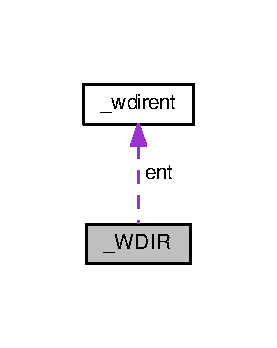
\includegraphics[width=133pt]{struct__WDIR__coll__graph}
\end{center}
\end{figure}
\subsection*{Public Attributes}
\begin{DoxyCompactItemize}
\item 
struct \hyperlink{struct__wdirent}{\+\_\+wdirent} {\bfseries ent}\hypertarget{struct__WDIR_a84ae1457352005f813ed4b3dc1994b62}{}\label{struct__WDIR_a84ae1457352005f813ed4b3dc1994b62}

\item 
W\+I\+N32\+\_\+\+F\+I\+N\+D\+\_\+\+D\+A\+T\+AW {\bfseries data}\hypertarget{struct__WDIR_a065b17b666ee06c4e8068d8accb0eef9}{}\label{struct__WDIR_a065b17b666ee06c4e8068d8accb0eef9}

\item 
int {\bfseries cached}\hypertarget{struct__WDIR_a9b7432df163d1e291ba5925347fd4af3}{}\label{struct__WDIR_a9b7432df163d1e291ba5925347fd4af3}

\item 
H\+A\+N\+D\+LE {\bfseries handle}\hypertarget{struct__WDIR_a694510e166fd3e797b3e15b9e4b3810a}{}\label{struct__WDIR_a694510e166fd3e797b3e15b9e4b3810a}

\item 
wchar\+\_\+t $\ast$ {\bfseries patt}\hypertarget{struct__WDIR_a700ff3a1096fb36452c571b0f55b4e60}{}\label{struct__WDIR_a700ff3a1096fb36452c571b0f55b4e60}

\end{DoxyCompactItemize}


The documentation for this struct was generated from the following file\+:\begin{DoxyCompactItemize}
\item 
Source/\+G\+\_\+\+System/direntw.\+h\end{DoxyCompactItemize}

\hypertarget{struct__wdirent}{}\section{\+\_\+wdirent Struct Reference}
\label{struct__wdirent}\index{\+\_\+wdirent@{\+\_\+wdirent}}
\subsection*{Public Attributes}
\begin{DoxyCompactItemize}
\item 
long {\bfseries d\+\_\+ino}\hypertarget{struct__wdirent_ac8cfaf294a0b6a49287d3f384c280c93}{}\label{struct__wdirent_ac8cfaf294a0b6a49287d3f384c280c93}

\item 
unsigned short {\bfseries d\+\_\+reclen}\hypertarget{struct__wdirent_aff7f360608e576cd18cf11f2caf13ef3}{}\label{struct__wdirent_aff7f360608e576cd18cf11f2caf13ef3}

\item 
size\+\_\+t {\bfseries d\+\_\+namlen}\hypertarget{struct__wdirent_a0050d6131e6fa90206903e216b38799e}{}\label{struct__wdirent_a0050d6131e6fa90206903e216b38799e}

\item 
int {\bfseries d\+\_\+type}\hypertarget{struct__wdirent_a3c3874604ffccbeeaffd96709763cc3b}{}\label{struct__wdirent_a3c3874604ffccbeeaffd96709763cc3b}

\item 
wchar\+\_\+t {\bfseries d\+\_\+name} \mbox{[}P\+A\+T\+H\+\_\+\+M\+AX\mbox{]}\hypertarget{struct__wdirent_a267f915cd36cad5969337a9192cab567}{}\label{struct__wdirent_a267f915cd36cad5969337a9192cab567}

\end{DoxyCompactItemize}


The documentation for this struct was generated from the following file\+:\begin{DoxyCompactItemize}
\item 
Source/\+G\+\_\+\+System/direntw.\+h\end{DoxyCompactItemize}

\hypertarget{classCatch_1_1Matchers_1_1Impl_1_1Generic_1_1AllOf}{}\section{Catch\+:\+:Matchers\+:\+:Impl\+:\+:Generic\+:\+:All\+Of$<$ ExpressionT $>$ Class Template Reference}
\label{classCatch_1_1Matchers_1_1Impl_1_1Generic_1_1AllOf}\index{Catch\+::\+Matchers\+::\+Impl\+::\+Generic\+::\+All\+Of$<$ Expression\+T $>$@{Catch\+::\+Matchers\+::\+Impl\+::\+Generic\+::\+All\+Of$<$ Expression\+T $>$}}


Inheritance diagram for Catch\+:\+:Matchers\+:\+:Impl\+:\+:Generic\+:\+:All\+Of$<$ ExpressionT $>$\+:
\nopagebreak
\begin{figure}[H]
\begin{center}
\leavevmode
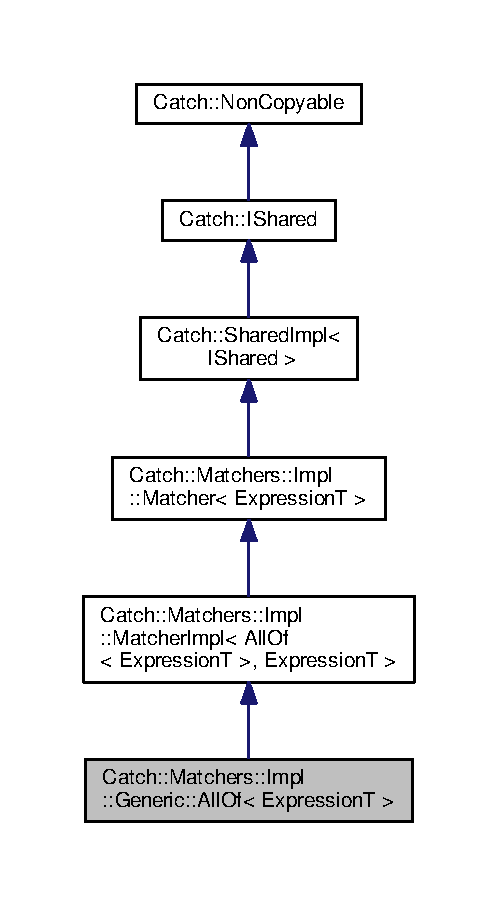
\includegraphics[width=239pt]{classCatch_1_1Matchers_1_1Impl_1_1Generic_1_1AllOf__inherit__graph}
\end{center}
\end{figure}


Collaboration diagram for Catch\+:\+:Matchers\+:\+:Impl\+:\+:Generic\+:\+:All\+Of$<$ ExpressionT $>$\+:
\nopagebreak
\begin{figure}[H]
\begin{center}
\leavevmode
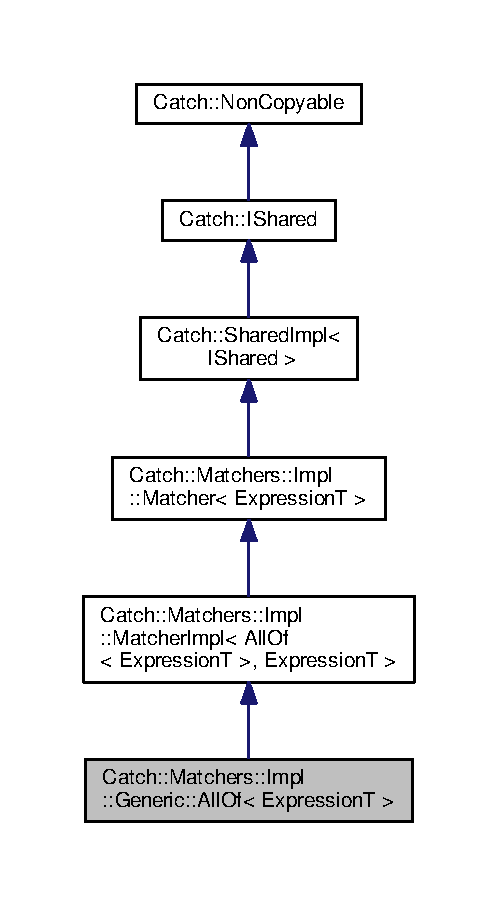
\includegraphics[width=239pt]{classCatch_1_1Matchers_1_1Impl_1_1Generic_1_1AllOf__coll__graph}
\end{center}
\end{figure}
\subsection*{Public Member Functions}
\begin{DoxyCompactItemize}
\item 
{\bfseries All\+Of} (\hyperlink{classCatch_1_1Matchers_1_1Impl_1_1Generic_1_1AllOf}{All\+Of} const \&other)\hypertarget{classCatch_1_1Matchers_1_1Impl_1_1Generic_1_1AllOf_a31f7c5e570e79bdf64064ee87c331a59}{}\label{classCatch_1_1Matchers_1_1Impl_1_1Generic_1_1AllOf_a31f7c5e570e79bdf64064ee87c331a59}

\item 
\hyperlink{classCatch_1_1Matchers_1_1Impl_1_1Generic_1_1AllOf}{All\+Of} \& {\bfseries add} (\hyperlink{structCatch_1_1Matchers_1_1Impl_1_1Matcher}{Matcher}$<$ ExpressionT $>$ const \&matcher)\hypertarget{classCatch_1_1Matchers_1_1Impl_1_1Generic_1_1AllOf_a8c5cd1e494ab697076da418ee72ac297}{}\label{classCatch_1_1Matchers_1_1Impl_1_1Generic_1_1AllOf_a8c5cd1e494ab697076da418ee72ac297}

\item 
virtual bool {\bfseries match} (ExpressionT const \&expr) const \hypertarget{classCatch_1_1Matchers_1_1Impl_1_1Generic_1_1AllOf_a04534d0ac9e089f4500c3c19054f11ce}{}\label{classCatch_1_1Matchers_1_1Impl_1_1Generic_1_1AllOf_a04534d0ac9e089f4500c3c19054f11ce}

\item 
virtual std\+::string {\bfseries to\+String} () const \hypertarget{classCatch_1_1Matchers_1_1Impl_1_1Generic_1_1AllOf_a9febc1e67acbeff62a32bcbfdc0c8fab}{}\label{classCatch_1_1Matchers_1_1Impl_1_1Generic_1_1AllOf_a9febc1e67acbeff62a32bcbfdc0c8fab}

\item 
\hyperlink{classCatch_1_1Matchers_1_1Impl_1_1Generic_1_1AllOf}{All\+Of} {\bfseries operator\&\&} (\hyperlink{structCatch_1_1Matchers_1_1Impl_1_1Matcher}{Matcher}$<$ ExpressionT $>$ const \&other) const \hypertarget{classCatch_1_1Matchers_1_1Impl_1_1Generic_1_1AllOf_ac2b4045ae39746852a0f603715ba1387}{}\label{classCatch_1_1Matchers_1_1Impl_1_1Generic_1_1AllOf_ac2b4045ae39746852a0f603715ba1387}

\end{DoxyCompactItemize}
\subsection*{Additional Inherited Members}


The documentation for this class was generated from the following file\+:\begin{DoxyCompactItemize}
\item 
Unit Tests/C\+A\+T\+C\+H.\+hpp\end{DoxyCompactItemize}

\hypertarget{classCatch_1_1Matchers_1_1Impl_1_1Generic_1_1AnyOf}{}\section{Catch\+:\+:Matchers\+:\+:Impl\+:\+:Generic\+:\+:Any\+Of$<$ ExpressionT $>$ Class Template Reference}
\label{classCatch_1_1Matchers_1_1Impl_1_1Generic_1_1AnyOf}\index{Catch\+::\+Matchers\+::\+Impl\+::\+Generic\+::\+Any\+Of$<$ Expression\+T $>$@{Catch\+::\+Matchers\+::\+Impl\+::\+Generic\+::\+Any\+Of$<$ Expression\+T $>$}}


Inheritance diagram for Catch\+:\+:Matchers\+:\+:Impl\+:\+:Generic\+:\+:Any\+Of$<$ ExpressionT $>$\+:
\nopagebreak
\begin{figure}[H]
\begin{center}
\leavevmode
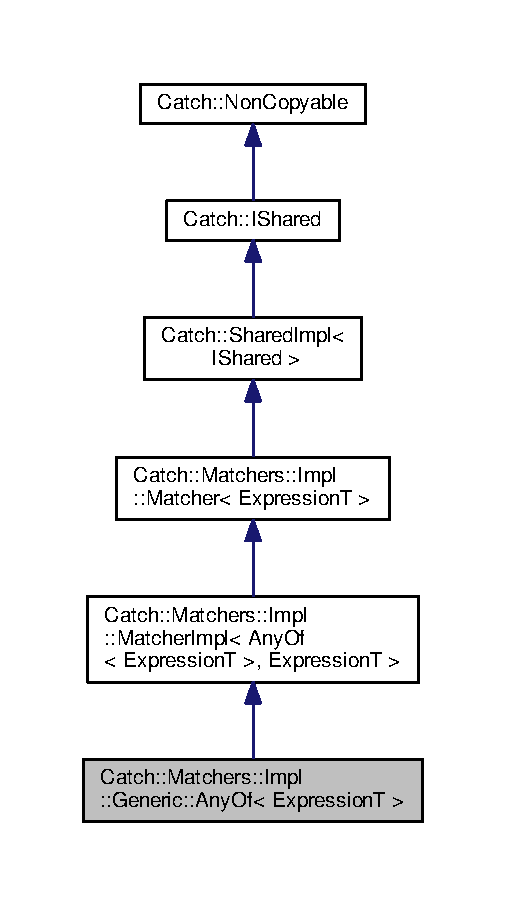
\includegraphics[width=243pt]{classCatch_1_1Matchers_1_1Impl_1_1Generic_1_1AnyOf__inherit__graph}
\end{center}
\end{figure}


Collaboration diagram for Catch\+:\+:Matchers\+:\+:Impl\+:\+:Generic\+:\+:Any\+Of$<$ ExpressionT $>$\+:
\nopagebreak
\begin{figure}[H]
\begin{center}
\leavevmode
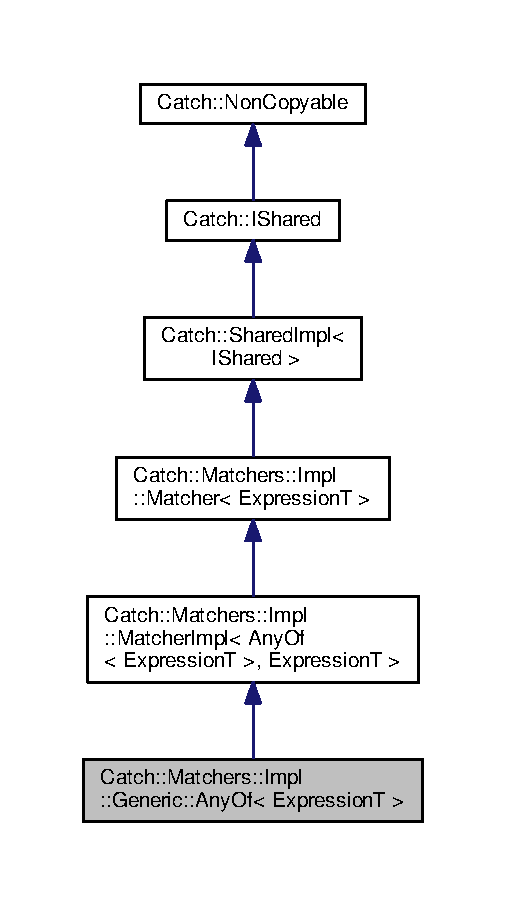
\includegraphics[width=243pt]{classCatch_1_1Matchers_1_1Impl_1_1Generic_1_1AnyOf__coll__graph}
\end{center}
\end{figure}
\subsection*{Public Member Functions}
\begin{DoxyCompactItemize}
\item 
{\bfseries Any\+Of} (\hyperlink{classCatch_1_1Matchers_1_1Impl_1_1Generic_1_1AnyOf}{Any\+Of} const \&other)\hypertarget{classCatch_1_1Matchers_1_1Impl_1_1Generic_1_1AnyOf_a74fbc05b32d334fcbfd0fae0163a404e}{}\label{classCatch_1_1Matchers_1_1Impl_1_1Generic_1_1AnyOf_a74fbc05b32d334fcbfd0fae0163a404e}

\item 
\hyperlink{classCatch_1_1Matchers_1_1Impl_1_1Generic_1_1AnyOf}{Any\+Of} \& {\bfseries add} (\hyperlink{structCatch_1_1Matchers_1_1Impl_1_1Matcher}{Matcher}$<$ ExpressionT $>$ const \&matcher)\hypertarget{classCatch_1_1Matchers_1_1Impl_1_1Generic_1_1AnyOf_a3bce94b627551e5f96c5f9c6060413f0}{}\label{classCatch_1_1Matchers_1_1Impl_1_1Generic_1_1AnyOf_a3bce94b627551e5f96c5f9c6060413f0}

\item 
virtual bool {\bfseries match} (ExpressionT const \&expr) const \hypertarget{classCatch_1_1Matchers_1_1Impl_1_1Generic_1_1AnyOf_a2f97a08338e12deba541043a57d73db9}{}\label{classCatch_1_1Matchers_1_1Impl_1_1Generic_1_1AnyOf_a2f97a08338e12deba541043a57d73db9}

\item 
virtual std\+::string {\bfseries to\+String} () const \hypertarget{classCatch_1_1Matchers_1_1Impl_1_1Generic_1_1AnyOf_a7ecc6ec08b2018a643923a9d450aa328}{}\label{classCatch_1_1Matchers_1_1Impl_1_1Generic_1_1AnyOf_a7ecc6ec08b2018a643923a9d450aa328}

\item 
\hyperlink{classCatch_1_1Matchers_1_1Impl_1_1Generic_1_1AnyOf}{Any\+Of} {\bfseries operator$\vert$$\vert$} (\hyperlink{structCatch_1_1Matchers_1_1Impl_1_1Matcher}{Matcher}$<$ ExpressionT $>$ const \&other) const \hypertarget{classCatch_1_1Matchers_1_1Impl_1_1Generic_1_1AnyOf_a07f4ea2ae366a6521a5d7bff4522e8bf}{}\label{classCatch_1_1Matchers_1_1Impl_1_1Generic_1_1AnyOf_a07f4ea2ae366a6521a5d7bff4522e8bf}

\end{DoxyCompactItemize}
\subsection*{Additional Inherited Members}


The documentation for this class was generated from the following file\+:\begin{DoxyCompactItemize}
\item 
Unit Tests/C\+A\+T\+C\+H.\+hpp\end{DoxyCompactItemize}

\hypertarget{classCatch_1_1Detail_1_1Approx}{}\section{Catch\+:\+:Detail\+:\+:Approx Class Reference}
\label{classCatch_1_1Detail_1_1Approx}\index{Catch\+::\+Detail\+::\+Approx@{Catch\+::\+Detail\+::\+Approx}}
\subsection*{Public Member Functions}
\begin{DoxyCompactItemize}
\item 
{\bfseries Approx} (double value)\hypertarget{classCatch_1_1Detail_1_1Approx_a1a8618ea8db08c66bd3d9fe8f74b957a}{}\label{classCatch_1_1Detail_1_1Approx_a1a8618ea8db08c66bd3d9fe8f74b957a}

\item 
{\bfseries Approx} (\hyperlink{classCatch_1_1Detail_1_1Approx}{Approx} const \&other)\hypertarget{classCatch_1_1Detail_1_1Approx_a807330c63266fc914abdf6e461255a54}{}\label{classCatch_1_1Detail_1_1Approx_a807330c63266fc914abdf6e461255a54}

\item 
\hyperlink{classCatch_1_1Detail_1_1Approx}{Approx} {\bfseries operator()} (double value)\hypertarget{classCatch_1_1Detail_1_1Approx_a48c9cbc28a05dc9dc8c3973b9eae2268}{}\label{classCatch_1_1Detail_1_1Approx_a48c9cbc28a05dc9dc8c3973b9eae2268}

\item 
\hyperlink{classCatch_1_1Detail_1_1Approx}{Approx} \& {\bfseries epsilon} (double new\+Epsilon)\hypertarget{classCatch_1_1Detail_1_1Approx_a05c50c3ad0a971fab19345b5d94979a9}{}\label{classCatch_1_1Detail_1_1Approx_a05c50c3ad0a971fab19345b5d94979a9}

\item 
\hyperlink{classCatch_1_1Detail_1_1Approx}{Approx} \& {\bfseries scale} (double new\+Scale)\hypertarget{classCatch_1_1Detail_1_1Approx_acd80f0737bf38112beacd5ca95bef113}{}\label{classCatch_1_1Detail_1_1Approx_acd80f0737bf38112beacd5ca95bef113}

\item 
std\+::string {\bfseries to\+String} () const \hypertarget{classCatch_1_1Detail_1_1Approx_adeb74b73506b3f6b2ba72aea15168fbe}{}\label{classCatch_1_1Detail_1_1Approx_adeb74b73506b3f6b2ba72aea15168fbe}

\end{DoxyCompactItemize}
\subsection*{Static Public Member Functions}
\begin{DoxyCompactItemize}
\item 
static \hyperlink{classCatch_1_1Detail_1_1Approx}{Approx} {\bfseries custom} ()\hypertarget{classCatch_1_1Detail_1_1Approx_aaf86dc0ee92272ac2d9839197a07951d}{}\label{classCatch_1_1Detail_1_1Approx_aaf86dc0ee92272ac2d9839197a07951d}

\end{DoxyCompactItemize}
\subsection*{Friends}
\begin{DoxyCompactItemize}
\item 
bool {\bfseries operator==} (double lhs, \hyperlink{classCatch_1_1Detail_1_1Approx}{Approx} const \&rhs)\hypertarget{classCatch_1_1Detail_1_1Approx_ac766f044f1c63f0c5997982baefd9049}{}\label{classCatch_1_1Detail_1_1Approx_ac766f044f1c63f0c5997982baefd9049}

\item 
bool {\bfseries operator==} (\hyperlink{classCatch_1_1Detail_1_1Approx}{Approx} const \&lhs, double rhs)\hypertarget{classCatch_1_1Detail_1_1Approx_a35999631e6cef569f9da9f3fa910db22}{}\label{classCatch_1_1Detail_1_1Approx_a35999631e6cef569f9da9f3fa910db22}

\item 
bool {\bfseries operator!=} (double lhs, \hyperlink{classCatch_1_1Detail_1_1Approx}{Approx} const \&rhs)\hypertarget{classCatch_1_1Detail_1_1Approx_a83b3763569a7ecc143c335b630be0e47}{}\label{classCatch_1_1Detail_1_1Approx_a83b3763569a7ecc143c335b630be0e47}

\item 
bool {\bfseries operator!=} (\hyperlink{classCatch_1_1Detail_1_1Approx}{Approx} const \&lhs, double rhs)\hypertarget{classCatch_1_1Detail_1_1Approx_a7497ef839f8026cc0edd6269a80f3e09}{}\label{classCatch_1_1Detail_1_1Approx_a7497ef839f8026cc0edd6269a80f3e09}

\end{DoxyCompactItemize}


The documentation for this class was generated from the following file\+:\begin{DoxyCompactItemize}
\item 
Unit Tests/C\+A\+T\+C\+H.\+hpp\end{DoxyCompactItemize}

\hypertarget{classAppWindow}{}\section{App\+Window Class Reference}
\label{classAppWindow}\index{App\+Window@{App\+Window}}


Map of Listeners to send event information to.  




Inheritance diagram for App\+Window\+:
\nopagebreak
\begin{figure}[H]
\begin{center}
\leavevmode
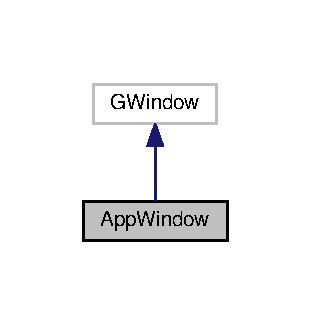
\includegraphics[width=149pt]{classAppWindow__inherit__graph}
\end{center}
\end{figure}


Collaboration diagram for App\+Window\+:
\nopagebreak
\begin{figure}[H]
\begin{center}
\leavevmode
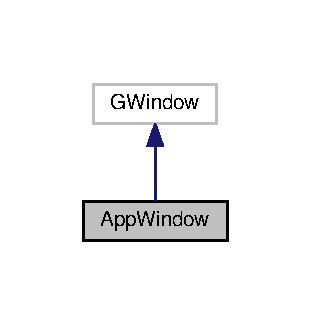
\includegraphics[width=149pt]{classAppWindow__coll__graph}
\end{center}
\end{figure}
\subsection*{Public Member Functions}
\begin{DoxyCompactItemize}
\item 
\hyperlink{namespaceGW_a67a839e3df7ea8a5c5686613a7a3de21}{G\+Return} {\bfseries Open\+Window} ()\hypertarget{classAppWindow_afb6034c67df3311832330de78ffb8363}{}\label{classAppWindow_afb6034c67df3311832330de78ffb8363}

\item 
\hyperlink{namespaceGW_a67a839e3df7ea8a5c5686613a7a3de21}{G\+Return} {\bfseries Process\+Window\+Events} ()\hypertarget{classAppWindow_a57bde2d7a148bbf7bfac8f21a7289ad4}{}\label{classAppWindow_a57bde2d7a148bbf7bfac8f21a7289ad4}

\item 
\hyperlink{namespaceGW_a67a839e3df7ea8a5c5686613a7a3de21}{G\+Return} {\bfseries Reconfigure\+Window} (int \+\_\+x, int \+\_\+y, int \+\_\+width, int \+\_\+height, G\+Window\+Style \+\_\+style)\hypertarget{classAppWindow_a16cadf1d2734d0e773ffdb2a40f263c5}{}\label{classAppWindow_a16cadf1d2734d0e773ffdb2a40f263c5}

\item 
\hyperlink{namespaceGW_a67a839e3df7ea8a5c5686613a7a3de21}{G\+Return} {\bfseries Init\+Window} (int \+\_\+x, int \+\_\+y, int \+\_\+width, int \+\_\+height, G\+Window\+Style \+\_\+style)\hypertarget{classAppWindow_a202f299c1f405d2fcbcc3ebd27b2b94f}{}\label{classAppWindow_a202f299c1f405d2fcbcc3ebd27b2b94f}

\item 
\hyperlink{namespaceGW_a67a839e3df7ea8a5c5686613a7a3de21}{G\+Return} {\bfseries Move\+Window} (int \+\_\+x, int \+\_\+y)\hypertarget{classAppWindow_adfc662614922cb2f81a837a0a272b4d6}{}\label{classAppWindow_adfc662614922cb2f81a837a0a272b4d6}

\item 
\hyperlink{namespaceGW_a67a839e3df7ea8a5c5686613a7a3de21}{G\+Return} {\bfseries Resize\+Window} (int \+\_\+width, int \+\_\+height)\hypertarget{classAppWindow_a4729069f577608a88a220491f3fe915b}{}\label{classAppWindow_a4729069f577608a88a220491f3fe915b}

\item 
\hyperlink{namespaceGW_a67a839e3df7ea8a5c5686613a7a3de21}{G\+Return} {\bfseries Maximize} ()\hypertarget{classAppWindow_a441624e699140c4fa7545a9235a7d518}{}\label{classAppWindow_a441624e699140c4fa7545a9235a7d518}

\item 
\hyperlink{namespaceGW_a67a839e3df7ea8a5c5686613a7a3de21}{G\+Return} {\bfseries Minimize} ()\hypertarget{classAppWindow_ae9e134ba36c205e64ebac37caf452261}{}\label{classAppWindow_ae9e134ba36c205e64ebac37caf452261}

\item 
\hyperlink{namespaceGW_a67a839e3df7ea8a5c5686613a7a3de21}{G\+Return} {\bfseries Change\+Window\+Style} (G\+Window\+Style \+\_\+style)\hypertarget{classAppWindow_a6895da18e8659cd9e038349dd767148c}{}\label{classAppWindow_a6895da18e8659cd9e038349dd767148c}

\item 
\hyperlink{namespaceGW_a67a839e3df7ea8a5c5686613a7a3de21}{G\+Return} {\bfseries Get\+Count} (unsigned int \&\+\_\+out\+Count)\hypertarget{classAppWindow_af7c0579ce4d7364f8ff80e01a6e5970d}{}\label{classAppWindow_af7c0579ce4d7364f8ff80e01a6e5970d}

\item 
\hyperlink{namespaceGW_a67a839e3df7ea8a5c5686613a7a3de21}{G\+Return} {\bfseries Increment\+Count} ()\hypertarget{classAppWindow_aedc73ad831ae0df2fdf0f1d115e80c27}{}\label{classAppWindow_aedc73ad831ae0df2fdf0f1d115e80c27}

\item 
\hyperlink{namespaceGW_a67a839e3df7ea8a5c5686613a7a3de21}{G\+Return} {\bfseries Decrement\+Count} ()\hypertarget{classAppWindow_a3e742c0356ae236d19259d4d6653160b}{}\label{classAppWindow_a3e742c0356ae236d19259d4d6653160b}

\item 
\hyperlink{namespaceGW_a67a839e3df7ea8a5c5686613a7a3de21}{G\+Return} {\bfseries Request\+Interface} (const \hyperlink{structGW_1_1GUUIID}{G\+U\+U\+I\+ID} \&\+\_\+interface\+ID, void $\ast$$\ast$\+\_\+output\+Interface)\hypertarget{classAppWindow_a69e61e9391fe44d390b28e9f93875acf}{}\label{classAppWindow_a69e61e9391fe44d390b28e9f93875acf}

\item 
\hyperlink{namespaceGW_a67a839e3df7ea8a5c5686613a7a3de21}{G\+Return} {\bfseries Register\+Listener} (G\+Listener $\ast$\+\_\+add\+Listener, unsigned long long \+\_\+event\+Mask)\hypertarget{classAppWindow_a8814a169073eff08ca452a523f829bcc}{}\label{classAppWindow_a8814a169073eff08ca452a523f829bcc}

\item 
\hyperlink{namespaceGW_a67a839e3df7ea8a5c5686613a7a3de21}{G\+Return} {\bfseries Deregister\+Listener} (G\+Listener $\ast$\+\_\+remove\+Listener)\hypertarget{classAppWindow_aa24326ca0883442aded7ebcd41812425}{}\label{classAppWindow_aa24326ca0883442aded7ebcd41812425}

\item 
int {\bfseries Get\+Width} ()\hypertarget{classAppWindow_a794be3cebb059335a3df241a283c41ef}{}\label{classAppWindow_a794be3cebb059335a3df241a283c41ef}

\item 
int {\bfseries Get\+Height} ()\hypertarget{classAppWindow_a71fec5e59bc2df0bccf78e86f56cb99f}{}\label{classAppWindow_a71fec5e59bc2df0bccf78e86f56cb99f}

\item 
int {\bfseries Get\+Client\+Width} ()\hypertarget{classAppWindow_aafdfb9b1f11d5bc502dd943838184126}{}\label{classAppWindow_aafdfb9b1f11d5bc502dd943838184126}

\item 
int {\bfseries Get\+Client\+Height} ()\hypertarget{classAppWindow_a0a6b3d1d6908f9e061259424811c71c8}{}\label{classAppWindow_a0a6b3d1d6908f9e061259424811c71c8}

\item 
int {\bfseries GetX} ()\hypertarget{classAppWindow_a5a00e9f08623efadad1f7df64e51366a}{}\label{classAppWindow_a5a00e9f08623efadad1f7df64e51366a}

\item 
int {\bfseries GetY} ()\hypertarget{classAppWindow_a1ca90dd2449e994af85ec7ee58abc07b}{}\label{classAppWindow_a1ca90dd2449e994af85ec7ee58abc07b}

\item 
\hyperlink{namespaceGW_a67a839e3df7ea8a5c5686613a7a3de21}{G\+Return} {\bfseries Get\+Client\+Top\+Left} (unsigned int \&\+\_\+outX, unsigned int \&\+\_\+outY)\hypertarget{classAppWindow_a2dca1ccca246528cd923a5e268de67fc}{}\label{classAppWindow_a2dca1ccca246528cd923a5e268de67fc}

\item 
void $\ast$ {\bfseries Get\+Window\+Handle} ()\hypertarget{classAppWindow_ab9538e9f0787ddced89e559b4e6004b0}{}\label{classAppWindow_ab9538e9f0787ddced89e559b4e6004b0}

\item 
bool {\bfseries Is\+Fullscreen} ()\hypertarget{classAppWindow_a7da02dcf2708946a743882fb9ee94458}{}\label{classAppWindow_a7da02dcf2708946a743882fb9ee94458}

\end{DoxyCompactItemize}


\subsection{Detailed Description}
Map of Listeners to send event information to. 

The documentation for this class was generated from the following file\+:\begin{DoxyCompactItemize}
\item 
Source/\+G\+\_\+\+System/G\+Window.\+cpp\end{DoxyCompactItemize}

\hypertarget{structCatch_1_1AssertionInfo}{}\section{Catch\+:\+:Assertion\+Info Struct Reference}
\label{structCatch_1_1AssertionInfo}\index{Catch\+::\+Assertion\+Info@{Catch\+::\+Assertion\+Info}}


Collaboration diagram for Catch\+:\+:Assertion\+Info\+:
\nopagebreak
\begin{figure}[H]
\begin{center}
\leavevmode
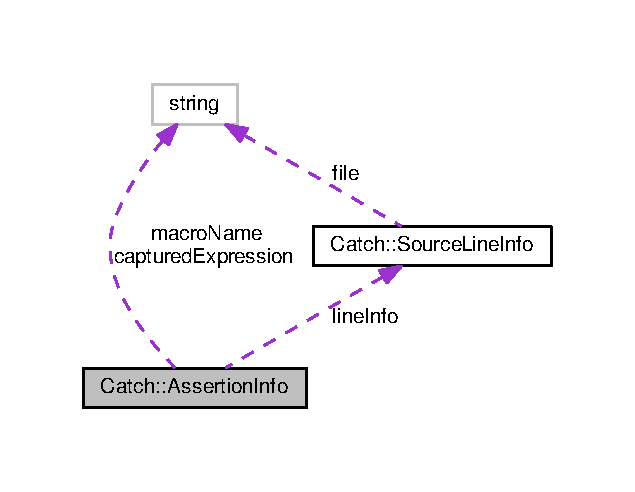
\includegraphics[width=305pt]{structCatch_1_1AssertionInfo__coll__graph}
\end{center}
\end{figure}
\subsection*{Public Member Functions}
\begin{DoxyCompactItemize}
\item 
{\bfseries Assertion\+Info} (std\+::string const \&\+\_\+macro\+Name, \hyperlink{structCatch_1_1SourceLineInfo}{Source\+Line\+Info} const \&\+\_\+line\+Info, std\+::string const \&\+\_\+captured\+Expression, Result\+Disposition\+::\+Flags \+\_\+result\+Disposition)\hypertarget{structCatch_1_1AssertionInfo_aaf6cc3eebd40391e54d37ed42953c73f}{}\label{structCatch_1_1AssertionInfo_aaf6cc3eebd40391e54d37ed42953c73f}

\end{DoxyCompactItemize}
\subsection*{Public Attributes}
\begin{DoxyCompactItemize}
\item 
std\+::string {\bfseries macro\+Name}\hypertarget{structCatch_1_1AssertionInfo_ac2e59e8c89e00eb3390768f50d540b18}{}\label{structCatch_1_1AssertionInfo_ac2e59e8c89e00eb3390768f50d540b18}

\item 
\hyperlink{structCatch_1_1SourceLineInfo}{Source\+Line\+Info} {\bfseries line\+Info}\hypertarget{structCatch_1_1AssertionInfo_a17bdbb404ba12658034f833be2f4c3e7}{}\label{structCatch_1_1AssertionInfo_a17bdbb404ba12658034f833be2f4c3e7}

\item 
std\+::string {\bfseries captured\+Expression}\hypertarget{structCatch_1_1AssertionInfo_af7c1d3cbfa346e9a303030fa0ef0cb54}{}\label{structCatch_1_1AssertionInfo_af7c1d3cbfa346e9a303030fa0ef0cb54}

\item 
Result\+Disposition\+::\+Flags {\bfseries result\+Disposition}\hypertarget{structCatch_1_1AssertionInfo_a60353b3632ab2f827162f2b2d6911073}{}\label{structCatch_1_1AssertionInfo_a60353b3632ab2f827162f2b2d6911073}

\end{DoxyCompactItemize}


The documentation for this struct was generated from the following file\+:\begin{DoxyCompactItemize}
\item 
Unit Tests/C\+A\+T\+C\+H.\+hpp\end{DoxyCompactItemize}

\hypertarget{classCatch_1_1AssertionResult}{}\section{Catch\+:\+:Assertion\+Result Class Reference}
\label{classCatch_1_1AssertionResult}\index{Catch\+::\+Assertion\+Result@{Catch\+::\+Assertion\+Result}}


Collaboration diagram for Catch\+:\+:Assertion\+Result\+:
\nopagebreak
\begin{figure}[H]
\begin{center}
\leavevmode
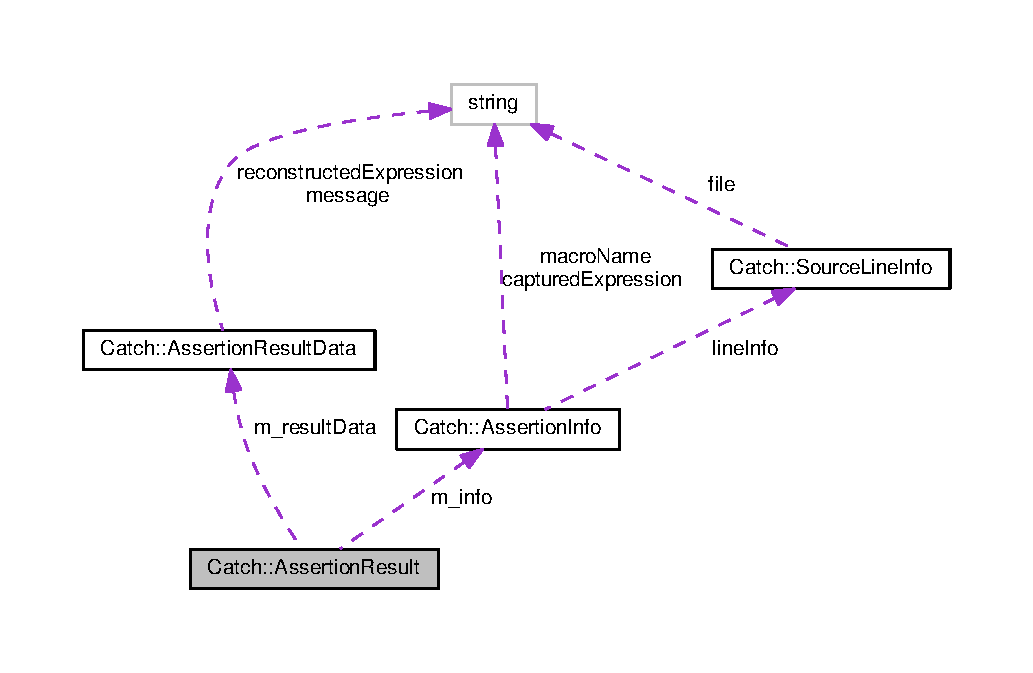
\includegraphics[width=350pt]{classCatch_1_1AssertionResult__coll__graph}
\end{center}
\end{figure}
\subsection*{Public Member Functions}
\begin{DoxyCompactItemize}
\item 
{\bfseries Assertion\+Result} (\hyperlink{structCatch_1_1AssertionInfo}{Assertion\+Info} const \&info, \hyperlink{structCatch_1_1AssertionResultData}{Assertion\+Result\+Data} const \&data)\hypertarget{classCatch_1_1AssertionResult_ab58aeec27052ba400633ed0e36cea692}{}\label{classCatch_1_1AssertionResult_ab58aeec27052ba400633ed0e36cea692}

\item 
bool {\bfseries is\+Ok} () const \hypertarget{classCatch_1_1AssertionResult_a70fb6aa62a38db3bdcafb4bb134afb21}{}\label{classCatch_1_1AssertionResult_a70fb6aa62a38db3bdcafb4bb134afb21}

\item 
bool {\bfseries succeeded} () const \hypertarget{classCatch_1_1AssertionResult_a5404062147930354afeb154de7cbaa7e}{}\label{classCatch_1_1AssertionResult_a5404062147930354afeb154de7cbaa7e}

\item 
Result\+Was\+::\+Of\+Type {\bfseries get\+Result\+Type} () const \hypertarget{classCatch_1_1AssertionResult_aa90bec8064879a62fcdc8e1079bcdba1}{}\label{classCatch_1_1AssertionResult_aa90bec8064879a62fcdc8e1079bcdba1}

\item 
bool {\bfseries has\+Expression} () const \hypertarget{classCatch_1_1AssertionResult_a45551f4f092c640ffce0cdd8a94f4b62}{}\label{classCatch_1_1AssertionResult_a45551f4f092c640ffce0cdd8a94f4b62}

\item 
bool {\bfseries has\+Message} () const \hypertarget{classCatch_1_1AssertionResult_ab22a1c9baa182aeb2549fffeb8294d9e}{}\label{classCatch_1_1AssertionResult_ab22a1c9baa182aeb2549fffeb8294d9e}

\item 
std\+::string {\bfseries get\+Expression} () const \hypertarget{classCatch_1_1AssertionResult_a6105300b90d66b5c11b69813f83d074d}{}\label{classCatch_1_1AssertionResult_a6105300b90d66b5c11b69813f83d074d}

\item 
std\+::string {\bfseries get\+Expression\+In\+Macro} () const \hypertarget{classCatch_1_1AssertionResult_ac368a7490af7669decd58efea7d7dc54}{}\label{classCatch_1_1AssertionResult_ac368a7490af7669decd58efea7d7dc54}

\item 
bool {\bfseries has\+Expanded\+Expression} () const \hypertarget{classCatch_1_1AssertionResult_a122c369bd49430a304e3eaebdf184f36}{}\label{classCatch_1_1AssertionResult_a122c369bd49430a304e3eaebdf184f36}

\item 
std\+::string {\bfseries get\+Expanded\+Expression} () const \hypertarget{classCatch_1_1AssertionResult_a675d074588875eb62b0b6e36e05d65e6}{}\label{classCatch_1_1AssertionResult_a675d074588875eb62b0b6e36e05d65e6}

\item 
std\+::string {\bfseries get\+Message} () const \hypertarget{classCatch_1_1AssertionResult_a9793bfc4d24678c8a013bda84a5aa905}{}\label{classCatch_1_1AssertionResult_a9793bfc4d24678c8a013bda84a5aa905}

\item 
\hyperlink{structCatch_1_1SourceLineInfo}{Source\+Line\+Info} {\bfseries get\+Source\+Info} () const \hypertarget{classCatch_1_1AssertionResult_a68b73fe982a97fe6432af679af1a2dad}{}\label{classCatch_1_1AssertionResult_a68b73fe982a97fe6432af679af1a2dad}

\item 
std\+::string {\bfseries get\+Test\+Macro\+Name} () const \hypertarget{classCatch_1_1AssertionResult_a2901d41b199258ff6a44571b147169dd}{}\label{classCatch_1_1AssertionResult_a2901d41b199258ff6a44571b147169dd}

\end{DoxyCompactItemize}
\subsection*{Protected Attributes}
\begin{DoxyCompactItemize}
\item 
\hyperlink{structCatch_1_1AssertionInfo}{Assertion\+Info} {\bfseries m\+\_\+info}\hypertarget{classCatch_1_1AssertionResult_a3e7236f73a51d6fc8bb9dfdefcee7772}{}\label{classCatch_1_1AssertionResult_a3e7236f73a51d6fc8bb9dfdefcee7772}

\item 
\hyperlink{structCatch_1_1AssertionResultData}{Assertion\+Result\+Data} {\bfseries m\+\_\+result\+Data}\hypertarget{classCatch_1_1AssertionResult_add3455b8bbedb0d643e18da67c66b4f7}{}\label{classCatch_1_1AssertionResult_add3455b8bbedb0d643e18da67c66b4f7}

\end{DoxyCompactItemize}


The documentation for this class was generated from the following file\+:\begin{DoxyCompactItemize}
\item 
Unit Tests/C\+A\+T\+C\+H.\+hpp\end{DoxyCompactItemize}

\hypertarget{structCatch_1_1AssertionResultData}{}\section{Catch\+:\+:Assertion\+Result\+Data Struct Reference}
\label{structCatch_1_1AssertionResultData}\index{Catch\+::\+Assertion\+Result\+Data@{Catch\+::\+Assertion\+Result\+Data}}


Collaboration diagram for Catch\+:\+:Assertion\+Result\+Data\+:
\nopagebreak
\begin{figure}[H]
\begin{center}
\leavevmode
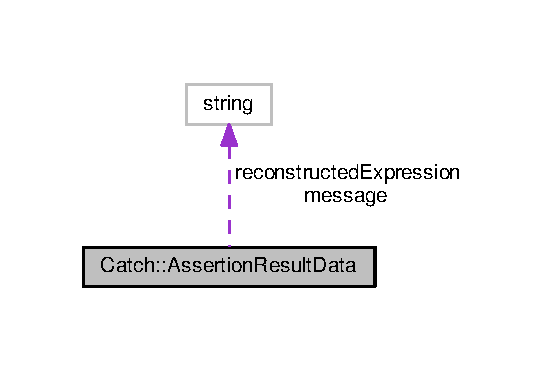
\includegraphics[width=262pt]{structCatch_1_1AssertionResultData__coll__graph}
\end{center}
\end{figure}
\subsection*{Public Attributes}
\begin{DoxyCompactItemize}
\item 
std\+::string {\bfseries reconstructed\+Expression}\hypertarget{structCatch_1_1AssertionResultData_a9e809d36fffbeb1c7d0cbe7382dd9595}{}\label{structCatch_1_1AssertionResultData_a9e809d36fffbeb1c7d0cbe7382dd9595}

\item 
std\+::string {\bfseries message}\hypertarget{structCatch_1_1AssertionResultData_ac34215803c4c4a88f795879f61c1f7b4}{}\label{structCatch_1_1AssertionResultData_ac34215803c4c4a88f795879f61c1f7b4}

\item 
Result\+Was\+::\+Of\+Type {\bfseries result\+Type}\hypertarget{structCatch_1_1AssertionResultData_a7ceab4a7ff722aec5587e3748caf66b7}{}\label{structCatch_1_1AssertionResultData_a7ceab4a7ff722aec5587e3748caf66b7}

\end{DoxyCompactItemize}


The documentation for this struct was generated from the following file\+:\begin{DoxyCompactItemize}
\item 
Unit Tests/C\+A\+T\+C\+H.\+hpp\end{DoxyCompactItemize}

\hypertarget{structCatch_1_1AutoReg}{}\section{Catch\+:\+:Auto\+Reg Struct Reference}
\label{structCatch_1_1AutoReg}\index{Catch\+::\+Auto\+Reg@{Catch\+::\+Auto\+Reg}}
\subsection*{Public Member Functions}
\begin{DoxyCompactItemize}
\item 
{\bfseries Auto\+Reg} (Test\+Function function, \hyperlink{structCatch_1_1SourceLineInfo}{Source\+Line\+Info} const \&line\+Info, \hyperlink{structCatch_1_1NameAndDesc}{Name\+And\+Desc} const \&name\+And\+Desc)\hypertarget{structCatch_1_1AutoReg_af224f4568d57b8652474df475a164a8c}{}\label{structCatch_1_1AutoReg_af224f4568d57b8652474df475a164a8c}

\item 
{\footnotesize template$<$typename C $>$ }\\{\bfseries Auto\+Reg} (void(C\+::$\ast$method)(), char const $\ast$class\+Name, \hyperlink{structCatch_1_1NameAndDesc}{Name\+And\+Desc} const \&name\+And\+Desc, \hyperlink{structCatch_1_1SourceLineInfo}{Source\+Line\+Info} const \&line\+Info)\hypertarget{structCatch_1_1AutoReg_a1bf9207fe0a02b46dc0ab1cc03cbe738}{}\label{structCatch_1_1AutoReg_a1bf9207fe0a02b46dc0ab1cc03cbe738}

\end{DoxyCompactItemize}


The documentation for this struct was generated from the following file\+:\begin{DoxyCompactItemize}
\item 
Unit Tests/C\+A\+T\+C\+H.\+hpp\end{DoxyCompactItemize}

\hypertarget{classCatch_1_1BetweenGenerator}{}\section{Catch\+:\+:Between\+Generator$<$ T $>$ Class Template Reference}
\label{classCatch_1_1BetweenGenerator}\index{Catch\+::\+Between\+Generator$<$ T $>$@{Catch\+::\+Between\+Generator$<$ T $>$}}


Inheritance diagram for Catch\+:\+:Between\+Generator$<$ T $>$\+:
\nopagebreak
\begin{figure}[H]
\begin{center}
\leavevmode
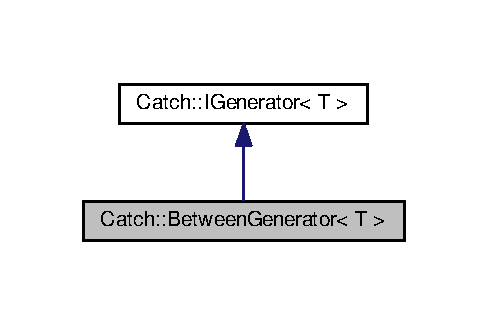
\includegraphics[width=234pt]{classCatch_1_1BetweenGenerator__inherit__graph}
\end{center}
\end{figure}


Collaboration diagram for Catch\+:\+:Between\+Generator$<$ T $>$\+:
\nopagebreak
\begin{figure}[H]
\begin{center}
\leavevmode
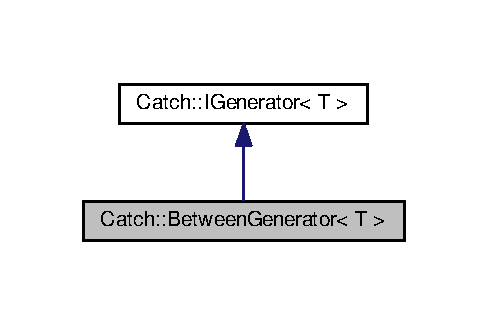
\includegraphics[width=234pt]{classCatch_1_1BetweenGenerator__coll__graph}
\end{center}
\end{figure}
\subsection*{Public Member Functions}
\begin{DoxyCompactItemize}
\item 
{\bfseries Between\+Generator} (T from, T to)\hypertarget{classCatch_1_1BetweenGenerator_a835a057d691ae37caef660624099b51c}{}\label{classCatch_1_1BetweenGenerator_a835a057d691ae37caef660624099b51c}

\item 
virtual T {\bfseries get\+Value} (std\+::size\+\_\+t index) const \hypertarget{classCatch_1_1BetweenGenerator_af83575d62cc727ca995446cff4d6c26c}{}\label{classCatch_1_1BetweenGenerator_af83575d62cc727ca995446cff4d6c26c}

\item 
virtual std\+::size\+\_\+t {\bfseries size} () const \hypertarget{classCatch_1_1BetweenGenerator_aa53a04a259e796ba2b5adabed79474b5}{}\label{classCatch_1_1BetweenGenerator_aa53a04a259e796ba2b5adabed79474b5}

\end{DoxyCompactItemize}


The documentation for this class was generated from the following file\+:\begin{DoxyCompactItemize}
\item 
Unit Tests/C\+A\+T\+C\+H.\+hpp\end{DoxyCompactItemize}

\hypertarget{structCatch_1_1Detail_1_1BorgType}{}\section{Catch\+:\+:Detail\+:\+:Borg\+Type Struct Reference}
\label{structCatch_1_1Detail_1_1BorgType}\index{Catch\+::\+Detail\+::\+Borg\+Type@{Catch\+::\+Detail\+::\+Borg\+Type}}
\subsection*{Public Member Functions}
\begin{DoxyCompactItemize}
\item 
{\footnotesize template$<$typename T $>$ }\\{\bfseries Borg\+Type} (T const \&)\hypertarget{structCatch_1_1Detail_1_1BorgType_a780a9946ed0d654f0bfc043c8fc505d8}{}\label{structCatch_1_1Detail_1_1BorgType_a780a9946ed0d654f0bfc043c8fc505d8}

\end{DoxyCompactItemize}


The documentation for this struct was generated from the following file\+:\begin{DoxyCompactItemize}
\item 
Unit Tests/C\+A\+T\+C\+H.\+hpp\end{DoxyCompactItemize}

\hypertarget{classBufferedInput}{}\section{Buffered\+Input Class Reference}
\label{classBufferedInput}\index{Buffered\+Input@{Buffered\+Input}}


Inheritance diagram for Buffered\+Input\+:
\nopagebreak
\begin{figure}[H]
\begin{center}
\leavevmode
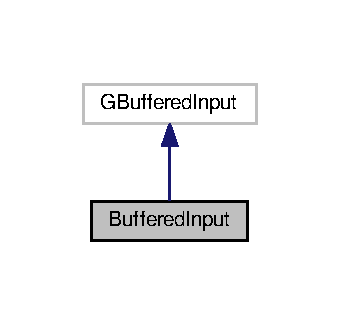
\includegraphics[width=163pt]{classBufferedInput__inherit__graph}
\end{center}
\end{figure}


Collaboration diagram for Buffered\+Input\+:
\nopagebreak
\begin{figure}[H]
\begin{center}
\leavevmode
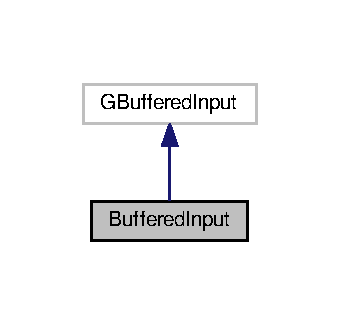
\includegraphics[width=163pt]{classBufferedInput__coll__graph}
\end{center}
\end{figure}
\subsection*{Public Member Functions}
\begin{DoxyCompactItemize}
\item 
void {\bfseries Input\+Thread} ()\hypertarget{classBufferedInput_a198931e0dc2e54a301b016fc51c5f7e5}{}\label{classBufferedInput_a198931e0dc2e54a301b016fc51c5f7e5}

\item 
\hyperlink{namespaceGW_a67a839e3df7ea8a5c5686613a7a3de21}{G\+Return} {\bfseries Initialize\+Windows} (void $\ast$\+\_\+data)\hypertarget{classBufferedInput_ab8594ef04a6bf4100b835c6ff8199d76}{}\label{classBufferedInput_ab8594ef04a6bf4100b835c6ff8199d76}

\item 
\hyperlink{namespaceGW_a67a839e3df7ea8a5c5686613a7a3de21}{G\+Return} {\bfseries Initialize\+Linux} (void $\ast$\+\_\+data)\hypertarget{classBufferedInput_ad82e212f6f9cef33ed3255cae15eaae7}{}\label{classBufferedInput_ad82e212f6f9cef33ed3255cae15eaae7}

\item 
\hyperlink{namespaceGW_a67a839e3df7ea8a5c5686613a7a3de21}{G\+Return} {\bfseries Initialize\+Mac} (void $\ast$\+\_\+data)\hypertarget{classBufferedInput_a18b419bcd05afc3cf306a2f3851d0c0f}{}\label{classBufferedInput_a18b419bcd05afc3cf306a2f3851d0c0f}

\item 
\hyperlink{namespaceGW_a67a839e3df7ea8a5c5686613a7a3de21}{G\+Return} {\bfseries Get\+Count} (unsigned int \&\+\_\+out\+Count)\hypertarget{classBufferedInput_af98a80ccd4b851192264e37aad15c3ab}{}\label{classBufferedInput_af98a80ccd4b851192264e37aad15c3ab}

\item 
\hyperlink{namespaceGW_a67a839e3df7ea8a5c5686613a7a3de21}{G\+Return} {\bfseries Increment\+Count} ()\hypertarget{classBufferedInput_a022aa95811f5426fe68ba04bbbefb413}{}\label{classBufferedInput_a022aa95811f5426fe68ba04bbbefb413}

\item 
\hyperlink{namespaceGW_a67a839e3df7ea8a5c5686613a7a3de21}{G\+Return} {\bfseries Decrement\+Count} ()\hypertarget{classBufferedInput_a74ca447adf3838cbea5c8e42e440a300}{}\label{classBufferedInput_a74ca447adf3838cbea5c8e42e440a300}

\item 
\hyperlink{namespaceGW_a67a839e3df7ea8a5c5686613a7a3de21}{G\+Return} {\bfseries Request\+Interface} (const \hyperlink{structGW_1_1GUUIID}{G\+U\+U\+I\+ID} \&\+\_\+interface\+ID, void $\ast$$\ast$\+\_\+output\+Interface)\hypertarget{classBufferedInput_a31065a70d0fb3fca9f458e7dd25c5df7}{}\label{classBufferedInput_a31065a70d0fb3fca9f458e7dd25c5df7}

\item 
\hyperlink{namespaceGW_a67a839e3df7ea8a5c5686613a7a3de21}{G\+Return} {\bfseries Register\+Listener} (\hyperlink{classGW_1_1CORE_1_1GListener}{G\+Listener} $\ast$\+\_\+add\+Listener, unsigned long long \+\_\+event\+Mask)\hypertarget{classBufferedInput_a210c1c6357ea98ed6cb443fc9e834dca}{}\label{classBufferedInput_a210c1c6357ea98ed6cb443fc9e834dca}

\item 
\hyperlink{namespaceGW_a67a839e3df7ea8a5c5686613a7a3de21}{G\+Return} {\bfseries Deregister\+Listener} (\hyperlink{classGW_1_1CORE_1_1GListener}{G\+Listener} $\ast$\+\_\+remove\+Listener)\hypertarget{classBufferedInput_ac3b002049f7542f8d6e2d87e29113f8c}{}\label{classBufferedInput_ac3b002049f7542f8d6e2d87e29113f8c}

\end{DoxyCompactItemize}


The documentation for this class was generated from the following file\+:\begin{DoxyCompactItemize}
\item 
Source/\+G\+\_\+\+System/G\+Buffered\+Input.\+cpp\end{DoxyCompactItemize}

\hypertarget{structCatch_1_1Matchers_1_1Impl_1_1StdString_1_1CasedString}{}\section{Catch\+:\+:Matchers\+:\+:Impl\+:\+:Std\+String\+:\+:Cased\+String Struct Reference}
\label{structCatch_1_1Matchers_1_1Impl_1_1StdString_1_1CasedString}\index{Catch\+::\+Matchers\+::\+Impl\+::\+Std\+String\+::\+Cased\+String@{Catch\+::\+Matchers\+::\+Impl\+::\+Std\+String\+::\+Cased\+String}}


Collaboration diagram for Catch\+:\+:Matchers\+:\+:Impl\+:\+:Std\+String\+:\+:Cased\+String\+:
\nopagebreak
\begin{figure}[H]
\begin{center}
\leavevmode
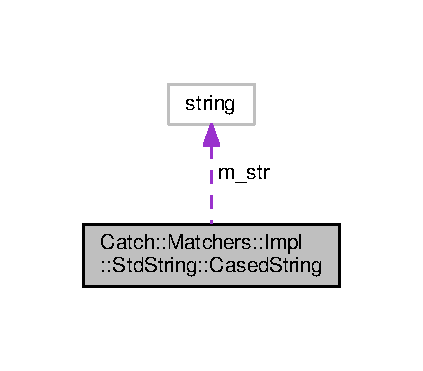
\includegraphics[width=203pt]{structCatch_1_1Matchers_1_1Impl_1_1StdString_1_1CasedString__coll__graph}
\end{center}
\end{figure}
\subsection*{Public Member Functions}
\begin{DoxyCompactItemize}
\item 
{\bfseries Cased\+String} (std\+::string const \&str, Case\+Sensitive\+::\+Choice case\+Sensitivity)\hypertarget{structCatch_1_1Matchers_1_1Impl_1_1StdString_1_1CasedString_aebd017c88423d8a11c62cff85754a22d}{}\label{structCatch_1_1Matchers_1_1Impl_1_1StdString_1_1CasedString_aebd017c88423d8a11c62cff85754a22d}

\item 
std\+::string {\bfseries adjust\+String} (std\+::string const \&str) const \hypertarget{structCatch_1_1Matchers_1_1Impl_1_1StdString_1_1CasedString_aaf5c4be8b3b8b317777d0e332d3733b5}{}\label{structCatch_1_1Matchers_1_1Impl_1_1StdString_1_1CasedString_aaf5c4be8b3b8b317777d0e332d3733b5}

\item 
std\+::string {\bfseries to\+String\+Suffix} () const \hypertarget{structCatch_1_1Matchers_1_1Impl_1_1StdString_1_1CasedString_ae5865fa1dd20c80498a094cae5459883}{}\label{structCatch_1_1Matchers_1_1Impl_1_1StdString_1_1CasedString_ae5865fa1dd20c80498a094cae5459883}

\end{DoxyCompactItemize}
\subsection*{Public Attributes}
\begin{DoxyCompactItemize}
\item 
Case\+Sensitive\+::\+Choice {\bfseries m\+\_\+case\+Sensitivity}\hypertarget{structCatch_1_1Matchers_1_1Impl_1_1StdString_1_1CasedString_af399ed93051d8981e298206dee6898b3}{}\label{structCatch_1_1Matchers_1_1Impl_1_1StdString_1_1CasedString_af399ed93051d8981e298206dee6898b3}

\item 
std\+::string {\bfseries m\+\_\+str}\hypertarget{structCatch_1_1Matchers_1_1Impl_1_1StdString_1_1CasedString_a9f8ce063a934330ac59bf8638f047e99}{}\label{structCatch_1_1Matchers_1_1Impl_1_1StdString_1_1CasedString_a9f8ce063a934330ac59bf8638f047e99}

\end{DoxyCompactItemize}


The documentation for this struct was generated from the following file\+:\begin{DoxyCompactItemize}
\item 
Unit Tests/C\+A\+T\+C\+H.\+hpp\end{DoxyCompactItemize}

\hypertarget{structCatch_1_1CaseSensitive}{}\section{Catch\+:\+:Case\+Sensitive Struct Reference}
\label{structCatch_1_1CaseSensitive}\index{Catch\+::\+Case\+Sensitive@{Catch\+::\+Case\+Sensitive}}
\subsection*{Public Types}
\begin{DoxyCompactItemize}
\item 
enum {\bfseries Choice} \{ {\bfseries Yes}, 
{\bfseries No}
 \}\hypertarget{structCatch_1_1CaseSensitive_aad49d3aee2d97066642fffa919685c6a}{}\label{structCatch_1_1CaseSensitive_aad49d3aee2d97066642fffa919685c6a}

\end{DoxyCompactItemize}


The documentation for this struct was generated from the following file\+:\begin{DoxyCompactItemize}
\item 
Unit Tests/C\+A\+T\+C\+H.\+hpp\end{DoxyCompactItemize}

\hypertarget{classCatch_1_1CompositeGenerator}{}\section{Catch\+:\+:Composite\+Generator$<$ T $>$ Class Template Reference}
\label{classCatch_1_1CompositeGenerator}\index{Catch\+::\+Composite\+Generator$<$ T $>$@{Catch\+::\+Composite\+Generator$<$ T $>$}}
\subsection*{Public Member Functions}
\begin{DoxyCompactItemize}
\item 
{\bfseries Composite\+Generator} (\hyperlink{classCatch_1_1CompositeGenerator}{Composite\+Generator} \&other)\hypertarget{classCatch_1_1CompositeGenerator_a21a7070a00e4a6fe021294c356692692}{}\label{classCatch_1_1CompositeGenerator_a21a7070a00e4a6fe021294c356692692}

\item 
\hyperlink{classCatch_1_1CompositeGenerator}{Composite\+Generator} \& {\bfseries set\+File\+Info} (const char $\ast$file\+Info)\hypertarget{classCatch_1_1CompositeGenerator_ac3c57cf4ca5472f440bf71e2936bcd4a}{}\label{classCatch_1_1CompositeGenerator_ac3c57cf4ca5472f440bf71e2936bcd4a}

\item 
{\bfseries operator T} () const \hypertarget{classCatch_1_1CompositeGenerator_aa3f627d84fb256df0404d19d7fd4b784}{}\label{classCatch_1_1CompositeGenerator_aa3f627d84fb256df0404d19d7fd4b784}

\item 
void {\bfseries add} (const \hyperlink{structCatch_1_1IGenerator}{I\+Generator}$<$ T $>$ $\ast$generator)\hypertarget{classCatch_1_1CompositeGenerator_af3774d42ad2d3453d089ca599efe0517}{}\label{classCatch_1_1CompositeGenerator_af3774d42ad2d3453d089ca599efe0517}

\item 
\hyperlink{classCatch_1_1CompositeGenerator}{Composite\+Generator} \& {\bfseries then} (\hyperlink{classCatch_1_1CompositeGenerator}{Composite\+Generator} \&other)\hypertarget{classCatch_1_1CompositeGenerator_a2e03f42df85cdd238aabd77a80b075d5}{}\label{classCatch_1_1CompositeGenerator_a2e03f42df85cdd238aabd77a80b075d5}

\item 
\hyperlink{classCatch_1_1CompositeGenerator}{Composite\+Generator} \& {\bfseries then} (T value)\hypertarget{classCatch_1_1CompositeGenerator_aefdc11bcfccdf07d2db5f0da3ed8758c}{}\label{classCatch_1_1CompositeGenerator_aefdc11bcfccdf07d2db5f0da3ed8758c}

\end{DoxyCompactItemize}


The documentation for this class was generated from the following file\+:\begin{DoxyCompactItemize}
\item 
Unit Tests/C\+A\+T\+C\+H.\+hpp\end{DoxyCompactItemize}

\hypertarget{structCatch_1_1Matchers_1_1Impl_1_1StdString_1_1Contains}{}\section{Catch\+:\+:Matchers\+:\+:Impl\+:\+:Std\+String\+:\+:Contains Struct Reference}
\label{structCatch_1_1Matchers_1_1Impl_1_1StdString_1_1Contains}\index{Catch\+::\+Matchers\+::\+Impl\+::\+Std\+String\+::\+Contains@{Catch\+::\+Matchers\+::\+Impl\+::\+Std\+String\+::\+Contains}}


Inheritance diagram for Catch\+:\+:Matchers\+:\+:Impl\+:\+:Std\+String\+:\+:Contains\+:
\nopagebreak
\begin{figure}[H]
\begin{center}
\leavevmode
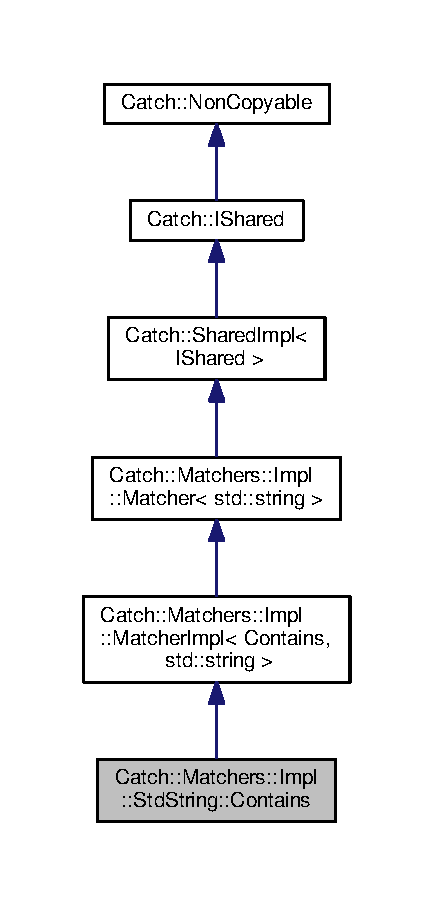
\includegraphics[width=208pt]{structCatch_1_1Matchers_1_1Impl_1_1StdString_1_1Contains__inherit__graph}
\end{center}
\end{figure}


Collaboration diagram for Catch\+:\+:Matchers\+:\+:Impl\+:\+:Std\+String\+:\+:Contains\+:
\nopagebreak
\begin{figure}[H]
\begin{center}
\leavevmode
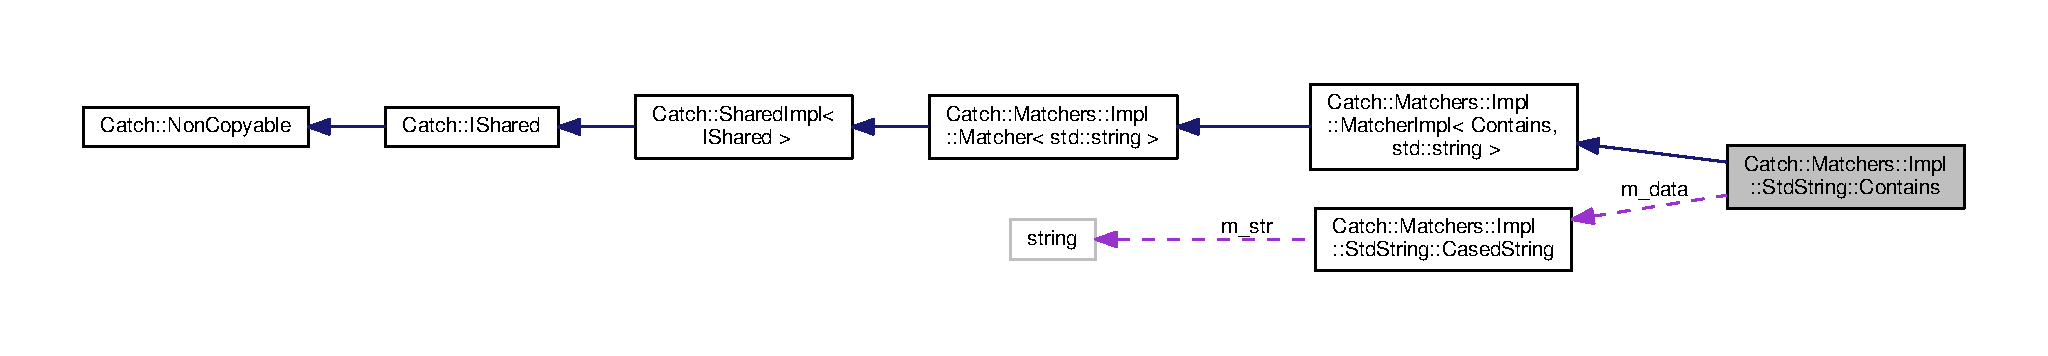
\includegraphics[width=350pt]{structCatch_1_1Matchers_1_1Impl_1_1StdString_1_1Contains__coll__graph}
\end{center}
\end{figure}
\subsection*{Public Member Functions}
\begin{DoxyCompactItemize}
\item 
{\bfseries Contains} (std\+::string const \&substr, Case\+Sensitive\+::\+Choice case\+Sensitivity=Case\+Sensitive\+::\+Yes)\hypertarget{structCatch_1_1Matchers_1_1Impl_1_1StdString_1_1Contains_a7a062d83bd3e3075929dbb55e1c24258}{}\label{structCatch_1_1Matchers_1_1Impl_1_1StdString_1_1Contains_a7a062d83bd3e3075929dbb55e1c24258}

\item 
{\bfseries Contains} (\hyperlink{structCatch_1_1Matchers_1_1Impl_1_1StdString_1_1Contains}{Contains} const \&other)\hypertarget{structCatch_1_1Matchers_1_1Impl_1_1StdString_1_1Contains_ad6b1ef653dfcb3bab43c43be043dc4e8}{}\label{structCatch_1_1Matchers_1_1Impl_1_1StdString_1_1Contains_ad6b1ef653dfcb3bab43c43be043dc4e8}

\item 
virtual bool {\bfseries match} (std\+::string const \&expr) const \hypertarget{structCatch_1_1Matchers_1_1Impl_1_1StdString_1_1Contains_aa27d823dea5770025a24424fc3355a6f}{}\label{structCatch_1_1Matchers_1_1Impl_1_1StdString_1_1Contains_aa27d823dea5770025a24424fc3355a6f}

\item 
virtual std\+::string {\bfseries to\+String} () const \hypertarget{structCatch_1_1Matchers_1_1Impl_1_1StdString_1_1Contains_a226755351f3598179925f3ab89d6def7}{}\label{structCatch_1_1Matchers_1_1Impl_1_1StdString_1_1Contains_a226755351f3598179925f3ab89d6def7}

\end{DoxyCompactItemize}
\subsection*{Public Attributes}
\begin{DoxyCompactItemize}
\item 
\hyperlink{structCatch_1_1Matchers_1_1Impl_1_1StdString_1_1CasedString}{Cased\+String} {\bfseries m\+\_\+data}\hypertarget{structCatch_1_1Matchers_1_1Impl_1_1StdString_1_1Contains_a419a9ecaeaa417d4987982402e08b3eb}{}\label{structCatch_1_1Matchers_1_1Impl_1_1StdString_1_1Contains_a419a9ecaeaa417d4987982402e08b3eb}

\end{DoxyCompactItemize}
\subsection*{Additional Inherited Members}


The documentation for this struct was generated from the following file\+:\begin{DoxyCompactItemize}
\item 
Unit Tests/C\+A\+T\+C\+H.\+hpp\end{DoxyCompactItemize}

\hypertarget{structCatch_1_1CopyableStream}{}\section{Catch\+:\+:Copyable\+Stream Struct Reference}
\label{structCatch_1_1CopyableStream}\index{Catch\+::\+Copyable\+Stream@{Catch\+::\+Copyable\+Stream}}
\subsection*{Public Member Functions}
\begin{DoxyCompactItemize}
\item 
{\bfseries Copyable\+Stream} (\hyperlink{structCatch_1_1CopyableStream}{Copyable\+Stream} const \&other)\hypertarget{structCatch_1_1CopyableStream_a0e72dc16240653f52c17106f4bf34da8}{}\label{structCatch_1_1CopyableStream_a0e72dc16240653f52c17106f4bf34da8}

\item 
\hyperlink{structCatch_1_1CopyableStream}{Copyable\+Stream} \& {\bfseries operator=} (\hyperlink{structCatch_1_1CopyableStream}{Copyable\+Stream} const \&other)\hypertarget{structCatch_1_1CopyableStream_a1760fa29b38011c5845171260bec0966}{}\label{structCatch_1_1CopyableStream_a1760fa29b38011c5845171260bec0966}

\end{DoxyCompactItemize}
\subsection*{Public Attributes}
\begin{DoxyCompactItemize}
\item 
std\+::ostringstream {\bfseries oss}\hypertarget{structCatch_1_1CopyableStream_ae123fb4d673e7d7a13a3c5f6bc5d426c}{}\label{structCatch_1_1CopyableStream_ae123fb4d673e7d7a13a3c5f6bc5d426c}

\end{DoxyCompactItemize}


The documentation for this struct was generated from the following file\+:\begin{DoxyCompactItemize}
\item 
Unit Tests/C\+A\+T\+C\+H.\+hpp\end{DoxyCompactItemize}

\hypertarget{structCatch_1_1Counts}{}\section{Catch\+:\+:Counts Struct Reference}
\label{structCatch_1_1Counts}\index{Catch\+::\+Counts@{Catch\+::\+Counts}}
\subsection*{Public Member Functions}
\begin{DoxyCompactItemize}
\item 
\hyperlink{structCatch_1_1Counts}{Counts} {\bfseries operator-\/} (\hyperlink{structCatch_1_1Counts}{Counts} const \&other) const \hypertarget{structCatch_1_1Counts_aedf86fefe33938d132a6981171cd83e6}{}\label{structCatch_1_1Counts_aedf86fefe33938d132a6981171cd83e6}

\item 
\hyperlink{structCatch_1_1Counts}{Counts} \& {\bfseries operator+=} (\hyperlink{structCatch_1_1Counts}{Counts} const \&other)\hypertarget{structCatch_1_1Counts_a322a89475cd2cc039140ef371e973677}{}\label{structCatch_1_1Counts_a322a89475cd2cc039140ef371e973677}

\item 
std\+::size\+\_\+t {\bfseries total} () const \hypertarget{structCatch_1_1Counts_a9125c662e30114e5c5cc94729b1e9e84}{}\label{structCatch_1_1Counts_a9125c662e30114e5c5cc94729b1e9e84}

\item 
bool {\bfseries all\+Passed} () const \hypertarget{structCatch_1_1Counts_adbbaca552f6017ce69e0d5dc5500bea4}{}\label{structCatch_1_1Counts_adbbaca552f6017ce69e0d5dc5500bea4}

\item 
bool {\bfseries all\+Ok} () const \hypertarget{structCatch_1_1Counts_ab2497c9dfc77be757a90225ea69595f5}{}\label{structCatch_1_1Counts_ab2497c9dfc77be757a90225ea69595f5}

\end{DoxyCompactItemize}
\subsection*{Public Attributes}
\begin{DoxyCompactItemize}
\item 
std\+::size\+\_\+t {\bfseries passed}\hypertarget{structCatch_1_1Counts_ad28daaf3de28006400208b6dd0c631e6}{}\label{structCatch_1_1Counts_ad28daaf3de28006400208b6dd0c631e6}

\item 
std\+::size\+\_\+t {\bfseries failed}\hypertarget{structCatch_1_1Counts_a19982a3817a3bc2c07f0290e71f497a3}{}\label{structCatch_1_1Counts_a19982a3817a3bc2c07f0290e71f497a3}

\item 
std\+::size\+\_\+t {\bfseries failed\+But\+Ok}\hypertarget{structCatch_1_1Counts_ac090973a2ff51394cd452718e75c073e}{}\label{structCatch_1_1Counts_ac090973a2ff51394cd452718e75c073e}

\end{DoxyCompactItemize}


The documentation for this struct was generated from the following file\+:\begin{DoxyCompactItemize}
\item 
Unit Tests/C\+A\+T\+C\+H.\+hpp\end{DoxyCompactItemize}

\hypertarget{structDIR}{}\section{D\+IR Struct Reference}
\label{structDIR}\index{D\+IR@{D\+IR}}


Collaboration diagram for D\+IR\+:\nopagebreak
\begin{figure}[H]
\begin{center}
\leavevmode
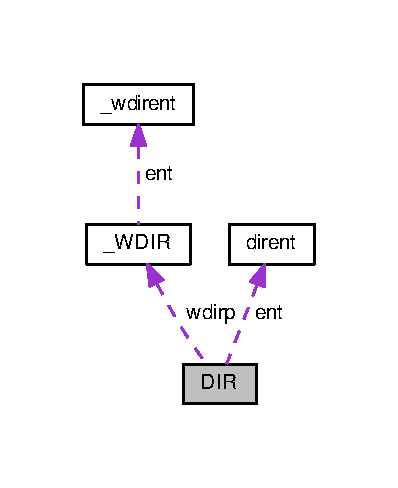
\includegraphics[width=191pt]{structDIR__coll__graph}
\end{center}
\end{figure}
\subsection*{Public Attributes}
\begin{DoxyCompactItemize}
\item 
struct \hyperlink{structdirent}{dirent} {\bfseries ent}\hypertarget{structDIR_a59e9f5211cbb2f8e5b2807ccfdd2a7fc}{}\label{structDIR_a59e9f5211cbb2f8e5b2807ccfdd2a7fc}

\item 
struct \hyperlink{struct__WDIR}{\+\_\+\+W\+D\+IR} $\ast$ {\bfseries wdirp}\hypertarget{structDIR_a29362d4a3d7f809d0f5418b26cac5d41}{}\label{structDIR_a29362d4a3d7f809d0f5418b26cac5d41}

\end{DoxyCompactItemize}


The documentation for this struct was generated from the following file\+:\begin{DoxyCompactItemize}
\item 
Source/\+G\+\_\+\+System/direntw.\+h\end{DoxyCompactItemize}

\hypertarget{structdirent}{}\section{dirent Struct Reference}
\label{structdirent}\index{dirent@{dirent}}
\subsection*{Public Attributes}
\begin{DoxyCompactItemize}
\item 
long {\bfseries d\+\_\+ino}\hypertarget{structdirent_acb6fecfb0e0f6fdc226dff8d56c3da4a}{}\label{structdirent_acb6fecfb0e0f6fdc226dff8d56c3da4a}

\item 
unsigned short {\bfseries d\+\_\+reclen}\hypertarget{structdirent_a90dc47836e8ef510437317876368859e}{}\label{structdirent_a90dc47836e8ef510437317876368859e}

\item 
size\+\_\+t {\bfseries d\+\_\+namlen}\hypertarget{structdirent_a09ced068b03cdb339e34840c8b709621}{}\label{structdirent_a09ced068b03cdb339e34840c8b709621}

\item 
int {\bfseries d\+\_\+type}\hypertarget{structdirent_ad6a736cb04c7295e8f97f708324b3500}{}\label{structdirent_ad6a736cb04c7295e8f97f708324b3500}

\item 
char {\bfseries d\+\_\+name} \mbox{[}P\+A\+T\+H\+\_\+\+M\+AX\mbox{]}\hypertarget{structdirent_a6c68ac080755453ec52de202e91de59b}{}\label{structdirent_a6c68ac080755453ec52de202e91de59b}

\end{DoxyCompactItemize}


The documentation for this struct was generated from the following file\+:\begin{DoxyCompactItemize}
\item 
Source/\+G\+\_\+\+System/direntw.\+h\end{DoxyCompactItemize}

\hypertarget{structCatch_1_1Matchers_1_1Impl_1_1StdString_1_1EndsWith}{}\section{Catch\+:\+:Matchers\+:\+:Impl\+:\+:Std\+String\+:\+:Ends\+With Struct Reference}
\label{structCatch_1_1Matchers_1_1Impl_1_1StdString_1_1EndsWith}\index{Catch\+::\+Matchers\+::\+Impl\+::\+Std\+String\+::\+Ends\+With@{Catch\+::\+Matchers\+::\+Impl\+::\+Std\+String\+::\+Ends\+With}}


Inheritance diagram for Catch\+:\+:Matchers\+:\+:Impl\+:\+:Std\+String\+:\+:Ends\+With\+:
\nopagebreak
\begin{figure}[H]
\begin{center}
\leavevmode
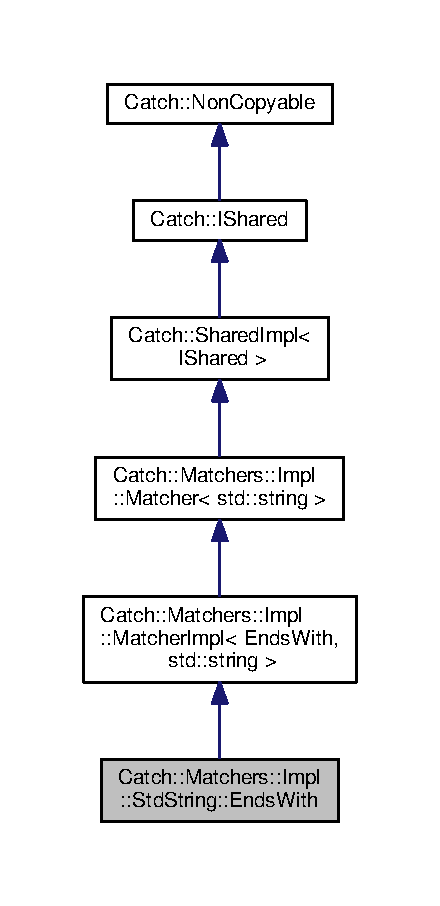
\includegraphics[width=211pt]{structCatch_1_1Matchers_1_1Impl_1_1StdString_1_1EndsWith__inherit__graph}
\end{center}
\end{figure}


Collaboration diagram for Catch\+:\+:Matchers\+:\+:Impl\+:\+:Std\+String\+:\+:Ends\+With\+:
\nopagebreak
\begin{figure}[H]
\begin{center}
\leavevmode
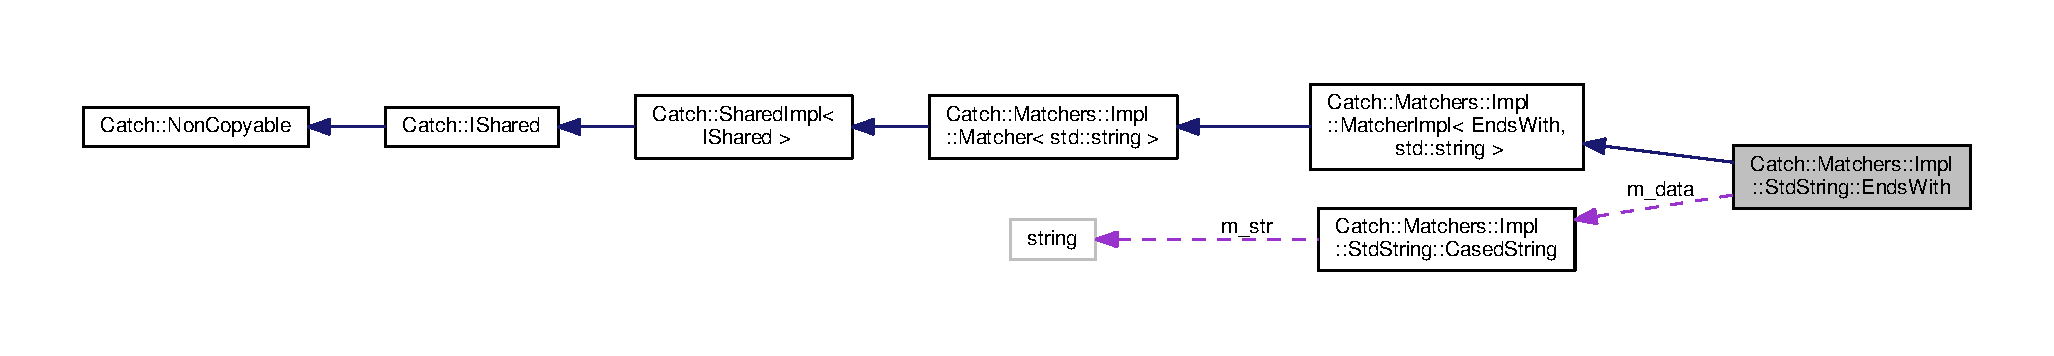
\includegraphics[width=350pt]{structCatch_1_1Matchers_1_1Impl_1_1StdString_1_1EndsWith__coll__graph}
\end{center}
\end{figure}
\subsection*{Public Member Functions}
\begin{DoxyCompactItemize}
\item 
{\bfseries Ends\+With} (std\+::string const \&substr, Case\+Sensitive\+::\+Choice case\+Sensitivity=Case\+Sensitive\+::\+Yes)\hypertarget{structCatch_1_1Matchers_1_1Impl_1_1StdString_1_1EndsWith_ae90c02ff06c9dd5e62218b2b521e8cab}{}\label{structCatch_1_1Matchers_1_1Impl_1_1StdString_1_1EndsWith_ae90c02ff06c9dd5e62218b2b521e8cab}

\item 
{\bfseries Ends\+With} (\hyperlink{structCatch_1_1Matchers_1_1Impl_1_1StdString_1_1EndsWith}{Ends\+With} const \&other)\hypertarget{structCatch_1_1Matchers_1_1Impl_1_1StdString_1_1EndsWith_a9321aac07fb17613a7993e99003b3be2}{}\label{structCatch_1_1Matchers_1_1Impl_1_1StdString_1_1EndsWith_a9321aac07fb17613a7993e99003b3be2}

\item 
virtual bool {\bfseries match} (std\+::string const \&expr) const \hypertarget{structCatch_1_1Matchers_1_1Impl_1_1StdString_1_1EndsWith_ad0e03d7f54ffa5859f84faebccf11e76}{}\label{structCatch_1_1Matchers_1_1Impl_1_1StdString_1_1EndsWith_ad0e03d7f54ffa5859f84faebccf11e76}

\item 
virtual std\+::string {\bfseries to\+String} () const \hypertarget{structCatch_1_1Matchers_1_1Impl_1_1StdString_1_1EndsWith_a54715c94c215a1fc5fb6336acf52eb06}{}\label{structCatch_1_1Matchers_1_1Impl_1_1StdString_1_1EndsWith_a54715c94c215a1fc5fb6336acf52eb06}

\end{DoxyCompactItemize}
\subsection*{Public Attributes}
\begin{DoxyCompactItemize}
\item 
\hyperlink{structCatch_1_1Matchers_1_1Impl_1_1StdString_1_1CasedString}{Cased\+String} {\bfseries m\+\_\+data}\hypertarget{structCatch_1_1Matchers_1_1Impl_1_1StdString_1_1EndsWith_a344d8433f3ba3e0de301ab16ed6dd746}{}\label{structCatch_1_1Matchers_1_1Impl_1_1StdString_1_1EndsWith_a344d8433f3ba3e0de301ab16ed6dd746}

\end{DoxyCompactItemize}
\subsection*{Additional Inherited Members}


The documentation for this struct was generated from the following file\+:\begin{DoxyCompactItemize}
\item 
Unit Tests/C\+A\+T\+C\+H.\+hpp\end{DoxyCompactItemize}

\hypertarget{structCatch_1_1Matchers_1_1Impl_1_1StdString_1_1Equals}{}\section{Catch\+:\+:Matchers\+:\+:Impl\+:\+:Std\+String\+:\+:Equals Struct Reference}
\label{structCatch_1_1Matchers_1_1Impl_1_1StdString_1_1Equals}\index{Catch\+::\+Matchers\+::\+Impl\+::\+Std\+String\+::\+Equals@{Catch\+::\+Matchers\+::\+Impl\+::\+Std\+String\+::\+Equals}}


Inheritance diagram for Catch\+:\+:Matchers\+:\+:Impl\+:\+:Std\+String\+:\+:Equals\+:
\nopagebreak
\begin{figure}[H]
\begin{center}
\leavevmode
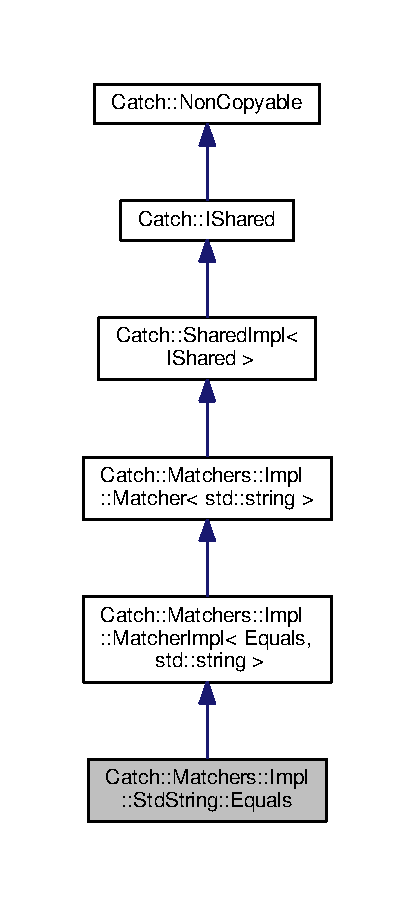
\includegraphics[width=199pt]{structCatch_1_1Matchers_1_1Impl_1_1StdString_1_1Equals__inherit__graph}
\end{center}
\end{figure}


Collaboration diagram for Catch\+:\+:Matchers\+:\+:Impl\+:\+:Std\+String\+:\+:Equals\+:
\nopagebreak
\begin{figure}[H]
\begin{center}
\leavevmode
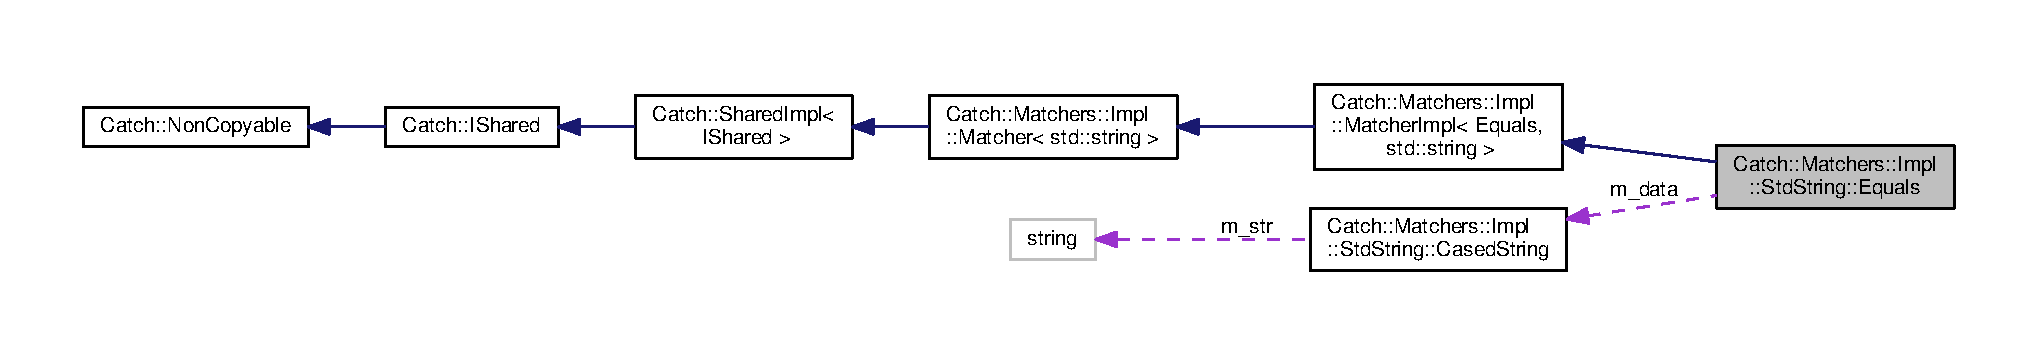
\includegraphics[width=350pt]{structCatch_1_1Matchers_1_1Impl_1_1StdString_1_1Equals__coll__graph}
\end{center}
\end{figure}
\subsection*{Public Member Functions}
\begin{DoxyCompactItemize}
\item 
{\bfseries Equals} (std\+::string const \&str, Case\+Sensitive\+::\+Choice case\+Sensitivity=Case\+Sensitive\+::\+Yes)\hypertarget{structCatch_1_1Matchers_1_1Impl_1_1StdString_1_1Equals_a5921d5ed75320fb64a678e3f1292a464}{}\label{structCatch_1_1Matchers_1_1Impl_1_1StdString_1_1Equals_a5921d5ed75320fb64a678e3f1292a464}

\item 
{\bfseries Equals} (\hyperlink{structCatch_1_1Matchers_1_1Impl_1_1StdString_1_1Equals}{Equals} const \&other)\hypertarget{structCatch_1_1Matchers_1_1Impl_1_1StdString_1_1Equals_acaa97de06aedf363ae803d65a975f5e4}{}\label{structCatch_1_1Matchers_1_1Impl_1_1StdString_1_1Equals_acaa97de06aedf363ae803d65a975f5e4}

\item 
virtual bool {\bfseries match} (std\+::string const \&expr) const \hypertarget{structCatch_1_1Matchers_1_1Impl_1_1StdString_1_1Equals_a00c8259a76c24da669e116662ededc70}{}\label{structCatch_1_1Matchers_1_1Impl_1_1StdString_1_1Equals_a00c8259a76c24da669e116662ededc70}

\item 
virtual std\+::string {\bfseries to\+String} () const \hypertarget{structCatch_1_1Matchers_1_1Impl_1_1StdString_1_1Equals_a7a09449ff2f858981caf3b1f6c36d270}{}\label{structCatch_1_1Matchers_1_1Impl_1_1StdString_1_1Equals_a7a09449ff2f858981caf3b1f6c36d270}

\end{DoxyCompactItemize}
\subsection*{Public Attributes}
\begin{DoxyCompactItemize}
\item 
\hyperlink{structCatch_1_1Matchers_1_1Impl_1_1StdString_1_1CasedString}{Cased\+String} {\bfseries m\+\_\+data}\hypertarget{structCatch_1_1Matchers_1_1Impl_1_1StdString_1_1Equals_ae09964b7ba291ce574b514a2ee3eddb0}{}\label{structCatch_1_1Matchers_1_1Impl_1_1StdString_1_1Equals_ae09964b7ba291ce574b514a2ee3eddb0}

\end{DoxyCompactItemize}
\subsection*{Additional Inherited Members}


The documentation for this struct was generated from the following file\+:\begin{DoxyCompactItemize}
\item 
Unit Tests/C\+A\+T\+C\+H.\+hpp\end{DoxyCompactItemize}

\hypertarget{classCatch_1_1Internal_1_1Evaluator}{}\section{Catch\+:\+:Internal\+:\+:Evaluator$<$ T1, T2, Op $>$ Class Template Reference}
\label{classCatch_1_1Internal_1_1Evaluator}\index{Catch\+::\+Internal\+::\+Evaluator$<$ T1, T2, Op $>$@{Catch\+::\+Internal\+::\+Evaluator$<$ T1, T2, Op $>$}}


The documentation for this class was generated from the following file\+:\begin{DoxyCompactItemize}
\item 
Unit Tests/C\+A\+T\+C\+H.\+hpp\end{DoxyCompactItemize}

\hypertarget{structCatch_1_1Internal_1_1Evaluator_3_01T1_00_01T2_00_01IsEqualTo_01_4}{}\section{Catch\+:\+:Internal\+:\+:Evaluator$<$ T1, T2, Is\+Equal\+To $>$ Struct Template Reference}
\label{structCatch_1_1Internal_1_1Evaluator_3_01T1_00_01T2_00_01IsEqualTo_01_4}\index{Catch\+::\+Internal\+::\+Evaluator$<$ T1, T2, Is\+Equal\+To $>$@{Catch\+::\+Internal\+::\+Evaluator$<$ T1, T2, Is\+Equal\+To $>$}}
\subsection*{Static Public Member Functions}
\begin{DoxyCompactItemize}
\item 
static bool {\bfseries evaluate} (T1 const \&lhs, T2 const \&rhs)\hypertarget{structCatch_1_1Internal_1_1Evaluator_3_01T1_00_01T2_00_01IsEqualTo_01_4_a166b2b7849247397e63fb2940481b217}{}\label{structCatch_1_1Internal_1_1Evaluator_3_01T1_00_01T2_00_01IsEqualTo_01_4_a166b2b7849247397e63fb2940481b217}

\end{DoxyCompactItemize}


The documentation for this struct was generated from the following file\+:\begin{DoxyCompactItemize}
\item 
Unit Tests/C\+A\+T\+C\+H.\+hpp\end{DoxyCompactItemize}

\hypertarget{structCatch_1_1Internal_1_1Evaluator_3_01T1_00_01T2_00_01IsGreaterThan_01_4}{}\section{Catch\+:\+:Internal\+:\+:Evaluator$<$ T1, T2, Is\+Greater\+Than $>$ Struct Template Reference}
\label{structCatch_1_1Internal_1_1Evaluator_3_01T1_00_01T2_00_01IsGreaterThan_01_4}\index{Catch\+::\+Internal\+::\+Evaluator$<$ T1, T2, Is\+Greater\+Than $>$@{Catch\+::\+Internal\+::\+Evaluator$<$ T1, T2, Is\+Greater\+Than $>$}}
\subsection*{Static Public Member Functions}
\begin{DoxyCompactItemize}
\item 
static bool {\bfseries evaluate} (T1 const \&lhs, T2 const \&rhs)\hypertarget{structCatch_1_1Internal_1_1Evaluator_3_01T1_00_01T2_00_01IsGreaterThan_01_4_a55745f74f09ac5c61bd3d592ca5560af}{}\label{structCatch_1_1Internal_1_1Evaluator_3_01T1_00_01T2_00_01IsGreaterThan_01_4_a55745f74f09ac5c61bd3d592ca5560af}

\end{DoxyCompactItemize}


The documentation for this struct was generated from the following file\+:\begin{DoxyCompactItemize}
\item 
Unit Tests/C\+A\+T\+C\+H.\+hpp\end{DoxyCompactItemize}

\hypertarget{structCatch_1_1Internal_1_1Evaluator_3_01T1_00_01T2_00_01IsGreaterThanOrEqualTo_01_4}{}\section{Catch\+:\+:Internal\+:\+:Evaluator$<$ T1, T2, Is\+Greater\+Than\+Or\+Equal\+To $>$ Struct Template Reference}
\label{structCatch_1_1Internal_1_1Evaluator_3_01T1_00_01T2_00_01IsGreaterThanOrEqualTo_01_4}\index{Catch\+::\+Internal\+::\+Evaluator$<$ T1, T2, Is\+Greater\+Than\+Or\+Equal\+To $>$@{Catch\+::\+Internal\+::\+Evaluator$<$ T1, T2, Is\+Greater\+Than\+Or\+Equal\+To $>$}}
\subsection*{Static Public Member Functions}
\begin{DoxyCompactItemize}
\item 
static bool {\bfseries evaluate} (T1 const \&lhs, T2 const \&rhs)\hypertarget{structCatch_1_1Internal_1_1Evaluator_3_01T1_00_01T2_00_01IsGreaterThanOrEqualTo_01_4_a5ba107c6da4292b6492a0e5e906f9484}{}\label{structCatch_1_1Internal_1_1Evaluator_3_01T1_00_01T2_00_01IsGreaterThanOrEqualTo_01_4_a5ba107c6da4292b6492a0e5e906f9484}

\end{DoxyCompactItemize}


The documentation for this struct was generated from the following file\+:\begin{DoxyCompactItemize}
\item 
Unit Tests/C\+A\+T\+C\+H.\+hpp\end{DoxyCompactItemize}

\hypertarget{structCatch_1_1Internal_1_1Evaluator_3_01T1_00_01T2_00_01IsLessThan_01_4}{}\section{Catch\+:\+:Internal\+:\+:Evaluator$<$ T1, T2, Is\+Less\+Than $>$ Struct Template Reference}
\label{structCatch_1_1Internal_1_1Evaluator_3_01T1_00_01T2_00_01IsLessThan_01_4}\index{Catch\+::\+Internal\+::\+Evaluator$<$ T1, T2, Is\+Less\+Than $>$@{Catch\+::\+Internal\+::\+Evaluator$<$ T1, T2, Is\+Less\+Than $>$}}
\subsection*{Static Public Member Functions}
\begin{DoxyCompactItemize}
\item 
static bool {\bfseries evaluate} (T1 const \&lhs, T2 const \&rhs)\hypertarget{structCatch_1_1Internal_1_1Evaluator_3_01T1_00_01T2_00_01IsLessThan_01_4_a75b2bcf80ce6f90218c145e2c3293d75}{}\label{structCatch_1_1Internal_1_1Evaluator_3_01T1_00_01T2_00_01IsLessThan_01_4_a75b2bcf80ce6f90218c145e2c3293d75}

\end{DoxyCompactItemize}


The documentation for this struct was generated from the following file\+:\begin{DoxyCompactItemize}
\item 
Unit Tests/C\+A\+T\+C\+H.\+hpp\end{DoxyCompactItemize}

\hypertarget{structCatch_1_1Internal_1_1Evaluator_3_01T1_00_01T2_00_01IsLessThanOrEqualTo_01_4}{}\section{Catch\+:\+:Internal\+:\+:Evaluator$<$ T1, T2, Is\+Less\+Than\+Or\+Equal\+To $>$ Struct Template Reference}
\label{structCatch_1_1Internal_1_1Evaluator_3_01T1_00_01T2_00_01IsLessThanOrEqualTo_01_4}\index{Catch\+::\+Internal\+::\+Evaluator$<$ T1, T2, Is\+Less\+Than\+Or\+Equal\+To $>$@{Catch\+::\+Internal\+::\+Evaluator$<$ T1, T2, Is\+Less\+Than\+Or\+Equal\+To $>$}}
\subsection*{Static Public Member Functions}
\begin{DoxyCompactItemize}
\item 
static bool {\bfseries evaluate} (T1 const \&lhs, T2 const \&rhs)\hypertarget{structCatch_1_1Internal_1_1Evaluator_3_01T1_00_01T2_00_01IsLessThanOrEqualTo_01_4_adf269a597e4d82d69f29bcb516297b9b}{}\label{structCatch_1_1Internal_1_1Evaluator_3_01T1_00_01T2_00_01IsLessThanOrEqualTo_01_4_adf269a597e4d82d69f29bcb516297b9b}

\end{DoxyCompactItemize}


The documentation for this struct was generated from the following file\+:\begin{DoxyCompactItemize}
\item 
Unit Tests/C\+A\+T\+C\+H.\+hpp\end{DoxyCompactItemize}

\hypertarget{structCatch_1_1Internal_1_1Evaluator_3_01T1_00_01T2_00_01IsNotEqualTo_01_4}{}\section{Catch\+:\+:Internal\+:\+:Evaluator$<$ T1, T2, Is\+Not\+Equal\+To $>$ Struct Template Reference}
\label{structCatch_1_1Internal_1_1Evaluator_3_01T1_00_01T2_00_01IsNotEqualTo_01_4}\index{Catch\+::\+Internal\+::\+Evaluator$<$ T1, T2, Is\+Not\+Equal\+To $>$@{Catch\+::\+Internal\+::\+Evaluator$<$ T1, T2, Is\+Not\+Equal\+To $>$}}
\subsection*{Static Public Member Functions}
\begin{DoxyCompactItemize}
\item 
static bool {\bfseries evaluate} (T1 const \&lhs, T2 const \&rhs)\hypertarget{structCatch_1_1Internal_1_1Evaluator_3_01T1_00_01T2_00_01IsNotEqualTo_01_4_a956a12d0f4a7dceb5a1ce914421ff945}{}\label{structCatch_1_1Internal_1_1Evaluator_3_01T1_00_01T2_00_01IsNotEqualTo_01_4_a956a12d0f4a7dceb5a1ce914421ff945}

\end{DoxyCompactItemize}


The documentation for this struct was generated from the following file\+:\begin{DoxyCompactItemize}
\item 
Unit Tests/C\+A\+T\+C\+H.\+hpp\end{DoxyCompactItemize}

\hypertarget{classCatch_1_1ExceptionTranslatorRegistrar}{}\section{Catch\+:\+:Exception\+Translator\+Registrar Class Reference}
\label{classCatch_1_1ExceptionTranslatorRegistrar}\index{Catch\+::\+Exception\+Translator\+Registrar@{Catch\+::\+Exception\+Translator\+Registrar}}
\subsection*{Public Member Functions}
\begin{DoxyCompactItemize}
\item 
{\footnotesize template$<$typename T $>$ }\\{\bfseries Exception\+Translator\+Registrar} (std\+::string($\ast$translate\+Function)(T \&))\hypertarget{classCatch_1_1ExceptionTranslatorRegistrar_aa73229de911f26b1df6c6c87c4d9e04e}{}\label{classCatch_1_1ExceptionTranslatorRegistrar_aa73229de911f26b1df6c6c87c4d9e04e}

\end{DoxyCompactItemize}


The documentation for this class was generated from the following file\+:\begin{DoxyCompactItemize}
\item 
Unit Tests/C\+A\+T\+C\+H.\+hpp\end{DoxyCompactItemize}

\hypertarget{classCatch_1_1ExpressionLhs}{}\section{Catch\+:\+:Expression\+Lhs$<$ T $>$ Class Template Reference}
\label{classCatch_1_1ExpressionLhs}\index{Catch\+::\+Expression\+Lhs$<$ T $>$@{Catch\+::\+Expression\+Lhs$<$ T $>$}}
\subsection*{Public Member Functions}
\begin{DoxyCompactItemize}
\item 
{\bfseries Expression\+Lhs} (\hyperlink{classCatch_1_1ResultBuilder}{Result\+Builder} \&rb, T lhs)\hypertarget{classCatch_1_1ExpressionLhs_aa829588def6146a94fb75de9c4cc482a}{}\label{classCatch_1_1ExpressionLhs_aa829588def6146a94fb75de9c4cc482a}

\item 
{\footnotesize template$<$typename RhsT $>$ }\\\hyperlink{classCatch_1_1ResultBuilder}{Result\+Builder} \& {\bfseries operator==} (RhsT const \&rhs)\hypertarget{classCatch_1_1ExpressionLhs_a2f7ad442c3e5e5764eee736345c40301}{}\label{classCatch_1_1ExpressionLhs_a2f7ad442c3e5e5764eee736345c40301}

\item 
{\footnotesize template$<$typename RhsT $>$ }\\\hyperlink{classCatch_1_1ResultBuilder}{Result\+Builder} \& {\bfseries operator!=} (RhsT const \&rhs)\hypertarget{classCatch_1_1ExpressionLhs_a44df9974cf20fcfda4e5b6b3c01d5f93}{}\label{classCatch_1_1ExpressionLhs_a44df9974cf20fcfda4e5b6b3c01d5f93}

\item 
{\footnotesize template$<$typename RhsT $>$ }\\\hyperlink{classCatch_1_1ResultBuilder}{Result\+Builder} \& {\bfseries operator$<$} (RhsT const \&rhs)\hypertarget{classCatch_1_1ExpressionLhs_a48428d358ddc89729e2e3407f4024dac}{}\label{classCatch_1_1ExpressionLhs_a48428d358ddc89729e2e3407f4024dac}

\item 
{\footnotesize template$<$typename RhsT $>$ }\\\hyperlink{classCatch_1_1ResultBuilder}{Result\+Builder} \& {\bfseries operator$>$} (RhsT const \&rhs)\hypertarget{classCatch_1_1ExpressionLhs_ad3602a7ad945c751004065b1007dc183}{}\label{classCatch_1_1ExpressionLhs_ad3602a7ad945c751004065b1007dc183}

\item 
{\footnotesize template$<$typename RhsT $>$ }\\\hyperlink{classCatch_1_1ResultBuilder}{Result\+Builder} \& {\bfseries operator$<$=} (RhsT const \&rhs)\hypertarget{classCatch_1_1ExpressionLhs_afd188990e8a14b49c308ce7a79056846}{}\label{classCatch_1_1ExpressionLhs_afd188990e8a14b49c308ce7a79056846}

\item 
{\footnotesize template$<$typename RhsT $>$ }\\\hyperlink{classCatch_1_1ResultBuilder}{Result\+Builder} \& {\bfseries operator$>$=} (RhsT const \&rhs)\hypertarget{classCatch_1_1ExpressionLhs_a21d30d6026ff2b1f86ddbd6b0a90d036}{}\label{classCatch_1_1ExpressionLhs_a21d30d6026ff2b1f86ddbd6b0a90d036}

\item 
\hyperlink{classCatch_1_1ResultBuilder}{Result\+Builder} \& {\bfseries operator==} (bool rhs)\hypertarget{classCatch_1_1ExpressionLhs_a6001030bcfbabc3981013ddffb3e3bb6}{}\label{classCatch_1_1ExpressionLhs_a6001030bcfbabc3981013ddffb3e3bb6}

\item 
\hyperlink{classCatch_1_1ResultBuilder}{Result\+Builder} \& {\bfseries operator!=} (bool rhs)\hypertarget{classCatch_1_1ExpressionLhs_a71e48da9a894962e8b32a8af5359a4df}{}\label{classCatch_1_1ExpressionLhs_a71e48da9a894962e8b32a8af5359a4df}

\item 
void {\bfseries end\+Expression} ()\hypertarget{classCatch_1_1ExpressionLhs_a13d2551a927790284fb5ddf1ee2c9079}{}\label{classCatch_1_1ExpressionLhs_a13d2551a927790284fb5ddf1ee2c9079}

\item 
{\footnotesize template$<$typename RhsT $>$ }\\S\+T\+A\+T\+I\+C\+\_\+\+A\+S\+S\+E\+R\+T\+\_\+\+Expression\+\_\+\+Too\+\_\+\+Complex\+\_\+\+Please\+\_\+\+Rewrite\+\_\+\+As\+\_\+\+Binary\+\_\+\+Comparison \& {\bfseries operator+} (RhsT const \&)\hypertarget{classCatch_1_1ExpressionLhs_a29ffb8417e977f0a98c0eb537a7ca5af}{}\label{classCatch_1_1ExpressionLhs_a29ffb8417e977f0a98c0eb537a7ca5af}

\item 
{\footnotesize template$<$typename RhsT $>$ }\\S\+T\+A\+T\+I\+C\+\_\+\+A\+S\+S\+E\+R\+T\+\_\+\+Expression\+\_\+\+Too\+\_\+\+Complex\+\_\+\+Please\+\_\+\+Rewrite\+\_\+\+As\+\_\+\+Binary\+\_\+\+Comparison \& {\bfseries operator-\/} (RhsT const \&)\hypertarget{classCatch_1_1ExpressionLhs_a19ef0a33442bb18efef1ec65102151d1}{}\label{classCatch_1_1ExpressionLhs_a19ef0a33442bb18efef1ec65102151d1}

\item 
{\footnotesize template$<$typename RhsT $>$ }\\S\+T\+A\+T\+I\+C\+\_\+\+A\+S\+S\+E\+R\+T\+\_\+\+Expression\+\_\+\+Too\+\_\+\+Complex\+\_\+\+Please\+\_\+\+Rewrite\+\_\+\+As\+\_\+\+Binary\+\_\+\+Comparison \& {\bfseries operator/} (RhsT const \&)\hypertarget{classCatch_1_1ExpressionLhs_a37d50565046ac9b1c9159a7c0cf88a1e}{}\label{classCatch_1_1ExpressionLhs_a37d50565046ac9b1c9159a7c0cf88a1e}

\item 
{\footnotesize template$<$typename RhsT $>$ }\\S\+T\+A\+T\+I\+C\+\_\+\+A\+S\+S\+E\+R\+T\+\_\+\+Expression\+\_\+\+Too\+\_\+\+Complex\+\_\+\+Please\+\_\+\+Rewrite\+\_\+\+As\+\_\+\+Binary\+\_\+\+Comparison \& {\bfseries operator$\ast$} (RhsT const \&)\hypertarget{classCatch_1_1ExpressionLhs_a9a94294c22449f62087862ef911e6291}{}\label{classCatch_1_1ExpressionLhs_a9a94294c22449f62087862ef911e6291}

\item 
{\footnotesize template$<$typename RhsT $>$ }\\S\+T\+A\+T\+I\+C\+\_\+\+A\+S\+S\+E\+R\+T\+\_\+\+Expression\+\_\+\+Too\+\_\+\+Complex\+\_\+\+Please\+\_\+\+Rewrite\+\_\+\+As\+\_\+\+Binary\+\_\+\+Comparison \& {\bfseries operator\&\&} (RhsT const \&)\hypertarget{classCatch_1_1ExpressionLhs_a7f022056ef4f25e716ab85846be6229f}{}\label{classCatch_1_1ExpressionLhs_a7f022056ef4f25e716ab85846be6229f}

\item 
{\footnotesize template$<$typename RhsT $>$ }\\S\+T\+A\+T\+I\+C\+\_\+\+A\+S\+S\+E\+R\+T\+\_\+\+Expression\+\_\+\+Too\+\_\+\+Complex\+\_\+\+Please\+\_\+\+Rewrite\+\_\+\+As\+\_\+\+Binary\+\_\+\+Comparison \& {\bfseries operator$\vert$$\vert$} (RhsT const \&)\hypertarget{classCatch_1_1ExpressionLhs_a6932b72da79d6c6b03d867772ceac61b}{}\label{classCatch_1_1ExpressionLhs_a6932b72da79d6c6b03d867772ceac61b}

\end{DoxyCompactItemize}


The documentation for this class was generated from the following file\+:\begin{DoxyCompactItemize}
\item 
Unit Tests/C\+A\+T\+C\+H.\+hpp\end{DoxyCompactItemize}

\hypertarget{structCatch_1_1Detail_1_1FalseType}{}\section{Catch\+:\+:Detail\+:\+:False\+Type Struct Reference}
\label{structCatch_1_1Detail_1_1FalseType}\index{Catch\+::\+Detail\+::\+False\+Type@{Catch\+::\+Detail\+::\+False\+Type}}
\subsection*{Public Attributes}
\begin{DoxyCompactItemize}
\item 
char {\bfseries sizer} \mbox{[}2\mbox{]}\hypertarget{structCatch_1_1Detail_1_1FalseType_abc1a730e197d6f7750ae8aaf47b63477}{}\label{structCatch_1_1Detail_1_1FalseType_abc1a730e197d6f7750ae8aaf47b63477}

\end{DoxyCompactItemize}


The documentation for this struct was generated from the following file\+:\begin{DoxyCompactItemize}
\item 
Unit Tests/C\+A\+T\+C\+H.\+hpp\end{DoxyCompactItemize}

\hypertarget{classFileIO}{}\section{File\+IO Class Reference}
\label{classFileIO}\index{File\+IO@{File\+IO}}


Inheritance diagram for File\+IO\+:\nopagebreak
\begin{figure}[H]
\begin{center}
\leavevmode
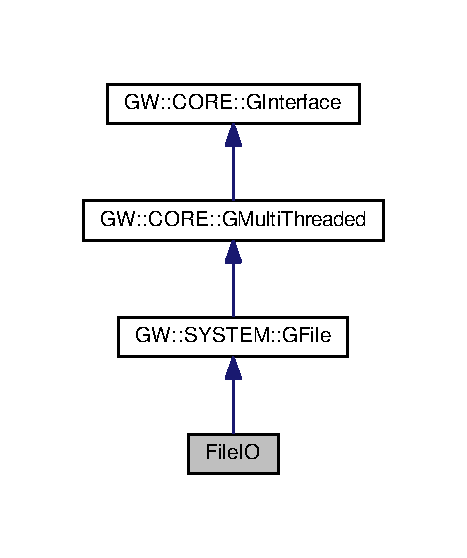
\includegraphics[width=224pt]{classFileIO__inherit__graph}
\end{center}
\end{figure}


Collaboration diagram for File\+IO\+:\nopagebreak
\begin{figure}[H]
\begin{center}
\leavevmode
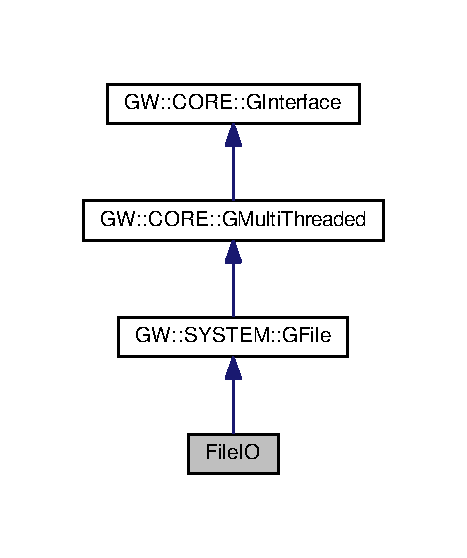
\includegraphics[width=224pt]{classFileIO__coll__graph}
\end{center}
\end{figure}
\subsection*{Public Member Functions}
\begin{DoxyCompactItemize}
\item 
\hyperlink{namespaceGW_a67a839e3df7ea8a5c5686613a7a3de21}{G\+W\+::\+G\+Return} \hyperlink{classFileIO_a0adeb88dd23bb5897e8315ab0029c835}{Open\+Binary\+Read} (const char $\ast$const \+\_\+file) override
\begin{DoxyCompactList}\small\item\em Opens a file for binary read. \end{DoxyCompactList}\item 
\hyperlink{namespaceGW_a67a839e3df7ea8a5c5686613a7a3de21}{G\+W\+::\+G\+Return} \hyperlink{classFileIO_a5cd87c21a72ae2dba21a9f3e50841e6e}{Open\+Binary\+Write} (const char $\ast$const \+\_\+file) override
\begin{DoxyCompactList}\small\item\em Opens a file for binary write with truncation. \end{DoxyCompactList}\item 
\hyperlink{namespaceGW_a67a839e3df7ea8a5c5686613a7a3de21}{G\+W\+::\+G\+Return} \hyperlink{classFileIO_ab26fc846b30446edf28ac922759c9e5e}{Append\+Binary\+Write} (const char $\ast$const \+\_\+file) override
\begin{DoxyCompactList}\small\item\em Opens a file for binary write with append. \end{DoxyCompactList}\item 
\hyperlink{namespaceGW_a67a839e3df7ea8a5c5686613a7a3de21}{G\+W\+::\+G\+Return} \hyperlink{classFileIO_a3d93902abce1baec299cd63891798681}{Open\+Text\+Read} (const char $\ast$const \+\_\+file) override
\begin{DoxyCompactList}\small\item\em Opens a file for text read. \end{DoxyCompactList}\item 
\hyperlink{namespaceGW_a67a839e3df7ea8a5c5686613a7a3de21}{G\+W\+::\+G\+Return} \hyperlink{classFileIO_a4e51443206e9cf97dcac28719dbeb23e}{Open\+Text\+Write} (const char $\ast$const \+\_\+file) override
\begin{DoxyCompactList}\small\item\em Opens a file for text write with truncation. \end{DoxyCompactList}\item 
\hyperlink{namespaceGW_a67a839e3df7ea8a5c5686613a7a3de21}{G\+W\+::\+G\+Return} \hyperlink{classFileIO_afd4e0d14b85d8c0aded66bd946c291f4}{Append\+Text\+Write} (const char $\ast$const \+\_\+file) override
\begin{DoxyCompactList}\small\item\em Opens a file for text write with append. \end{DoxyCompactList}\item 
\hyperlink{namespaceGW_a67a839e3df7ea8a5c5686613a7a3de21}{G\+W\+::\+G\+Return} \hyperlink{classFileIO_a6d849348b4255304b9a1c0c2bd4cd231}{Write} (const char $\ast$const \+\_\+in\+Data, unsigned int \+\_\+num\+Bytes) override
\begin{DoxyCompactList}\small\item\em Writes binary data to the currently opened file. \end{DoxyCompactList}\item 
\hyperlink{namespaceGW_a67a839e3df7ea8a5c5686613a7a3de21}{G\+W\+::\+G\+Return} \hyperlink{classFileIO_adb5270ace70c0189525a7c21c5be31b9}{Read} (char $\ast$\+\_\+out\+Data, unsigned int \+\_\+num\+Bytes) override
\begin{DoxyCompactList}\small\item\em Reads binary from the currently opened file. \end{DoxyCompactList}\item 
\hyperlink{namespaceGW_a67a839e3df7ea8a5c5686613a7a3de21}{G\+W\+::\+G\+Return} \hyperlink{classFileIO_af76c68078333756f887d7298fe9c3492}{Write\+Line} (const char $\ast$const \+\_\+in\+Data) override
\begin{DoxyCompactList}\small\item\em Writes text to the currently opened file. \end{DoxyCompactList}\item 
\hyperlink{namespaceGW_a67a839e3df7ea8a5c5686613a7a3de21}{G\+W\+::\+G\+Return} \hyperlink{classFileIO_a2178a711eb984539cefe6d651a7167fb}{Read\+Line} (char $\ast$\+\_\+out\+Data, unsigned int \+\_\+out\+Data\+Size, char \+\_\+delimiter) override
\begin{DoxyCompactList}\small\item\em Reads text to the currently opened file. \end{DoxyCompactList}\item 
\hyperlink{namespaceGW_a67a839e3df7ea8a5c5686613a7a3de21}{G\+W\+::\+G\+Return} \hyperlink{classFileIO_a906610c8653ba8ca476dc46679851590}{Close\+File} () override
\begin{DoxyCompactList}\small\item\em Flushes and closes the current file. \end{DoxyCompactList}\item 
\hyperlink{namespaceGW_a67a839e3df7ea8a5c5686613a7a3de21}{G\+W\+::\+G\+Return} \hyperlink{classFileIO_a8e5afdb1a734f37e422ff0147561a3a1}{Flush\+File} () override
\begin{DoxyCompactList}\small\item\em Flushes the current file. \end{DoxyCompactList}\item 
\hyperlink{namespaceGW_a67a839e3df7ea8a5c5686613a7a3de21}{G\+W\+::\+G\+Return} \hyperlink{classFileIO_a8332ededccf4034fd83509d9513a2635}{Set\+Current\+Working\+Directory} (const char $\ast$const \+\_\+dir) override
\begin{DoxyCompactList}\small\item\em Changes the current working directory. \end{DoxyCompactList}\item 
\hyperlink{namespaceGW_a67a839e3df7ea8a5c5686613a7a3de21}{G\+W\+::\+G\+Return} \hyperlink{classFileIO_a41a1859ffe3ebd76005f264af0b1ea66}{Get\+Current\+Working\+Directory} (char $\ast$\+\_\+dir, unsigned int \+\_\+dir\+Size) override
\begin{DoxyCompactList}\small\item\em Retrieves the absolute path of the current working directory. \end{DoxyCompactList}\item 
\hyperlink{namespaceGW_a67a839e3df7ea8a5c5686613a7a3de21}{G\+W\+::\+G\+Return} \hyperlink{classFileIO_ae331f6c02948720d9cc5bcd2700d8cf7}{Get\+Directory\+Size} (unsigned int \&\+\_\+out\+Size) override
\begin{DoxyCompactList}\small\item\em Gets the number of files in the current working directory. \end{DoxyCompactList}\item 
\hyperlink{namespaceGW_a67a839e3df7ea8a5c5686613a7a3de21}{G\+W\+::\+G\+Return} \hyperlink{classFileIO_afd1b77afed3d853aaa01f14ecbc6b0e0}{Get\+Files\+From\+Directory} (char $\ast$\+\_\+out\+Files\mbox{[}$\,$\mbox{]}, unsigned int \+\_\+num\+Files, unsigned int \+\_\+file\+Name\+Size) override
\begin{DoxyCompactList}\small\item\em Gets the names of all files in the current working directory. \end{DoxyCompactList}\item 
\hyperlink{namespaceGW_a67a839e3df7ea8a5c5686613a7a3de21}{G\+W\+::\+G\+Return} \hyperlink{classFileIO_a91ee3ceabd5d6097eed85466c26d2adb}{Get\+File\+Size} (const char $\ast$const \+\_\+file, unsigned int \&\+\_\+out\+Size) override
\begin{DoxyCompactList}\small\item\em Gets the size of the specified file in bytes. \end{DoxyCompactList}\item 
\hyperlink{namespaceGW_a67a839e3df7ea8a5c5686613a7a3de21}{G\+W\+::\+G\+Return} \hyperlink{classFileIO_a20566e320ec4cc0d5615bc3bc1fa3013}{Get\+Count} (unsigned int \&\+\_\+out\+Count) override
\begin{DoxyCompactList}\small\item\em Return the total number of active references to this object. \end{DoxyCompactList}\item 
\hyperlink{namespaceGW_a67a839e3df7ea8a5c5686613a7a3de21}{G\+W\+::\+G\+Return} \hyperlink{classFileIO_a9f2c9a4d13577e14a2c94b0e9617d80b}{Increment\+Count} () override
\begin{DoxyCompactList}\small\item\em Increase the total number of active references to this object. \end{DoxyCompactList}\item 
\hyperlink{namespaceGW_a67a839e3df7ea8a5c5686613a7a3de21}{G\+W\+::\+G\+Return} \hyperlink{classFileIO_ab7e4806ca819c3fcdeeb40a2af5f0298}{Decrement\+Count} () override
\begin{DoxyCompactList}\small\item\em Decrease the total number of active references to this object. \end{DoxyCompactList}\item 
\hyperlink{namespaceGW_a67a839e3df7ea8a5c5686613a7a3de21}{G\+W\+::\+G\+Return} \hyperlink{classFileIO_a3fb39527fac479474c6ef5045dbc1551}{Request\+Interface} (const \hyperlink{structGW_1_1GUUIID}{G\+W\+::\+G\+U\+U\+I\+ID} \&\+\_\+interface\+ID, void $\ast$$\ast$\+\_\+output\+Interface) override
\begin{DoxyCompactList}\small\item\em Requests an interface that may or may not be supported by this object. \end{DoxyCompactList}\item 
\hyperlink{namespaceGW_a67a839e3df7ea8a5c5686613a7a3de21}{G\+W\+::\+G\+Return} {\bfseries Init} ()\hypertarget{classFileIO_a1c24bf6f35d30462fd918e5ee1a44033}{}\label{classFileIO_a1c24bf6f35d30462fd918e5ee1a44033}

\end{DoxyCompactItemize}


\subsection{Member Function Documentation}
\index{File\+IO@{File\+IO}!Append\+Binary\+Write@{Append\+Binary\+Write}}
\index{Append\+Binary\+Write@{Append\+Binary\+Write}!File\+IO@{File\+IO}}
\subsubsection[{\texorpdfstring{Append\+Binary\+Write(const char $\ast$const \+\_\+file) override}{AppendBinaryWrite(const char *const _file) override}}]{\setlength{\rightskip}{0pt plus 5cm}{\bf G\+W\+::\+G\+Return} File\+I\+O\+::\+Append\+Binary\+Write (
\begin{DoxyParamCaption}
\item[{const char $\ast$const}]{\+\_\+file}
\end{DoxyParamCaption}
)\hspace{0.3cm}{\ttfamily [override]}, {\ttfamily [virtual]}}\hypertarget{classFileIO_ab26fc846b30446edf28ac922759c9e5e}{}\label{classFileIO_ab26fc846b30446edf28ac922759c9e5e}


Opens a file for binary write with append. 

The file name passed into the function should be passed like it is a relative path. The function will look in the current working directory for the file. If the file is not found in the current working directory, the file will be created in the current working directory. File can now be written to with \hyperlink{classFileIO_a6d849348b4255304b9a1c0c2bd4cd231}{Write()}.


\begin{DoxyParams}[1]{Parameters}
\mbox{\tt in}  & {\em \+\_\+file} & The file name of the file to open.\\
\hline
\end{DoxyParams}

\begin{DoxyRetVals}{Return values}
{\em S\+U\+C\+C\+E\+SS} & Succesfully opened the file. \\
\hline
{\em F\+A\+I\+L\+U\+RE} & A file is already open or the file could not be found/created. \\
\hline
{\em I\+N\+V\+A\+L\+I\+D\+\_\+\+A\+R\+G\+U\+M\+E\+NT} & A nullptr was passed in. \\
\hline
\end{DoxyRetVals}


Implements \hyperlink{classGW_1_1SYSTEM_1_1GFile_a63311236692181f99fd393fe8e1ca9fc}{G\+W\+::\+S\+Y\+S\+T\+E\+M\+::\+G\+File}.

\index{File\+IO@{File\+IO}!Append\+Text\+Write@{Append\+Text\+Write}}
\index{Append\+Text\+Write@{Append\+Text\+Write}!File\+IO@{File\+IO}}
\subsubsection[{\texorpdfstring{Append\+Text\+Write(const char $\ast$const \+\_\+file) override}{AppendTextWrite(const char *const _file) override}}]{\setlength{\rightskip}{0pt plus 5cm}{\bf G\+W\+::\+G\+Return} File\+I\+O\+::\+Append\+Text\+Write (
\begin{DoxyParamCaption}
\item[{const char $\ast$const}]{\+\_\+file}
\end{DoxyParamCaption}
)\hspace{0.3cm}{\ttfamily [override]}, {\ttfamily [virtual]}}\hypertarget{classFileIO_afd4e0d14b85d8c0aded66bd946c291f4}{}\label{classFileIO_afd4e0d14b85d8c0aded66bd946c291f4}


Opens a file for text write with append. 

The file name passed into the function should be passed like it is a relative path. The function will look in the current working directory for the file. If the file is not found in the current working directory, the file will be created in the current working directory. File can now be written to with \hyperlink{classFileIO_a6d849348b4255304b9a1c0c2bd4cd231}{Write()}.


\begin{DoxyParams}[1]{Parameters}
\mbox{\tt in}  & {\em \+\_\+file} & The file name of the file to open.\\
\hline
\end{DoxyParams}

\begin{DoxyRetVals}{Return values}
{\em S\+U\+C\+C\+E\+SS} & Succesfully opened the file. \\
\hline
{\em F\+A\+I\+L\+U\+RE} & A file is already open or the file could not be found/created. \\
\hline
{\em I\+N\+V\+A\+L\+I\+D\+\_\+\+A\+R\+G\+U\+M\+E\+NT} & A nullptr was passed in. \\
\hline
\end{DoxyRetVals}


Implements \hyperlink{classGW_1_1SYSTEM_1_1GFile_a72e40b3234a2384738d8db6e958f4782}{G\+W\+::\+S\+Y\+S\+T\+E\+M\+::\+G\+File}.

\index{File\+IO@{File\+IO}!Close\+File@{Close\+File}}
\index{Close\+File@{Close\+File}!File\+IO@{File\+IO}}
\subsubsection[{\texorpdfstring{Close\+File() override}{CloseFile() override}}]{\setlength{\rightskip}{0pt plus 5cm}{\bf G\+W\+::\+G\+Return} File\+I\+O\+::\+Close\+File (
\begin{DoxyParamCaption}
{}
\end{DoxyParamCaption}
)\hspace{0.3cm}{\ttfamily [override]}, {\ttfamily [virtual]}}\hypertarget{classFileIO_a906610c8653ba8ca476dc46679851590}{}\label{classFileIO_a906610c8653ba8ca476dc46679851590}


Flushes and closes the current file. 


\begin{DoxyRetVals}{Return values}
{\em S\+U\+C\+C\+E\+SS} & File successfully flushed and closed. \\
\hline
{\em F\+A\+I\+L\+U\+RE} & A file is not currently open. \\
\hline
\end{DoxyRetVals}


Implements \hyperlink{classGW_1_1SYSTEM_1_1GFile_ae661d107c461145bb095dcfc76519f54}{G\+W\+::\+S\+Y\+S\+T\+E\+M\+::\+G\+File}.

\index{File\+IO@{File\+IO}!Decrement\+Count@{Decrement\+Count}}
\index{Decrement\+Count@{Decrement\+Count}!File\+IO@{File\+IO}}
\subsubsection[{\texorpdfstring{Decrement\+Count() override}{DecrementCount() override}}]{\setlength{\rightskip}{0pt plus 5cm}{\bf G\+W\+::\+G\+Return} File\+I\+O\+::\+Decrement\+Count (
\begin{DoxyParamCaption}
{}
\end{DoxyParamCaption}
)\hspace{0.3cm}{\ttfamily [override]}, {\ttfamily [virtual]}}\hypertarget{classFileIO_ab7e4806ca819c3fcdeeb40a2af5f0298}{}\label{classFileIO_ab7e4806ca819c3fcdeeb40a2af5f0298}


Decrease the total number of active references to this object. 

Once the internal count reaches zero this object will be deallocated and your pointer will become invalid.


\begin{DoxyRetVals}{Return values}
{\em S\+U\+C\+C\+E\+SS} & Successfully decremented the internal reference count. \\
\hline
{\em F\+A\+I\+L\+U\+RE} & Decrementing of internal reference count would underflow the value. \\
\hline
\end{DoxyRetVals}


Implements \hyperlink{classGW_1_1CORE_1_1GInterface_a19a368c77ad0aa7f49b5a4f772f173ba}{G\+W\+::\+C\+O\+R\+E\+::\+G\+Interface}.

\index{File\+IO@{File\+IO}!Flush\+File@{Flush\+File}}
\index{Flush\+File@{Flush\+File}!File\+IO@{File\+IO}}
\subsubsection[{\texorpdfstring{Flush\+File() override}{FlushFile() override}}]{\setlength{\rightskip}{0pt plus 5cm}{\bf G\+W\+::\+G\+Return} File\+I\+O\+::\+Flush\+File (
\begin{DoxyParamCaption}
{}
\end{DoxyParamCaption}
)\hspace{0.3cm}{\ttfamily [override]}, {\ttfamily [virtual]}}\hypertarget{classFileIO_a8e5afdb1a734f37e422ff0147561a3a1}{}\label{classFileIO_a8e5afdb1a734f37e422ff0147561a3a1}


Flushes the current file. 


\begin{DoxyRetVals}{Return values}
{\em S\+U\+C\+C\+E\+SS} & File successfully flushed. \\
\hline
{\em F\+A\+I\+L\+U\+RE} & A file is not currently open. \\
\hline
\end{DoxyRetVals}


Implements \hyperlink{classGW_1_1SYSTEM_1_1GFile_ae3105b637ef87af268722a696b8657a9}{G\+W\+::\+S\+Y\+S\+T\+E\+M\+::\+G\+File}.

\index{File\+IO@{File\+IO}!Get\+Count@{Get\+Count}}
\index{Get\+Count@{Get\+Count}!File\+IO@{File\+IO}}
\subsubsection[{\texorpdfstring{Get\+Count(unsigned int \&\+\_\+out\+Count) override}{GetCount(unsigned int &_outCount) override}}]{\setlength{\rightskip}{0pt plus 5cm}{\bf G\+W\+::\+G\+Return} File\+I\+O\+::\+Get\+Count (
\begin{DoxyParamCaption}
\item[{unsigned int \&}]{\+\_\+out\+Count}
\end{DoxyParamCaption}
)\hspace{0.3cm}{\ttfamily [override]}, {\ttfamily [virtual]}}\hypertarget{classFileIO_a20566e320ec4cc0d5615bc3bc1fa3013}{}\label{classFileIO_a20566e320ec4cc0d5615bc3bc1fa3013}


Return the total number of active references to this object. 


\begin{DoxyParams}[1]{Parameters}
\mbox{\tt out}  & {\em \+\_\+out\+Count} & The total number of active references of this object.\\
\hline
\end{DoxyParams}

\begin{DoxyRetVals}{Return values}
{\em S\+U\+C\+C\+E\+SS} & Successfully ran. \\
\hline
{\em F\+A\+I\+L\+U\+RE} & Either class does not exist or the internal reference count is corrupt. \\
\hline
\end{DoxyRetVals}


Implements \hyperlink{classGW_1_1CORE_1_1GInterface_aacf5834174a7024f8a3c361122ee9e76}{G\+W\+::\+C\+O\+R\+E\+::\+G\+Interface}.

\index{File\+IO@{File\+IO}!Get\+Current\+Working\+Directory@{Get\+Current\+Working\+Directory}}
\index{Get\+Current\+Working\+Directory@{Get\+Current\+Working\+Directory}!File\+IO@{File\+IO}}
\subsubsection[{\texorpdfstring{Get\+Current\+Working\+Directory(char $\ast$\+\_\+dir, unsigned int \+\_\+dir\+Size) override}{GetCurrentWorkingDirectory(char *_dir, unsigned int _dirSize) override}}]{\setlength{\rightskip}{0pt plus 5cm}{\bf G\+W\+::\+G\+Return} File\+I\+O\+::\+Get\+Current\+Working\+Directory (
\begin{DoxyParamCaption}
\item[{char $\ast$}]{\+\_\+out\+Dir, }
\item[{unsigned int}]{\+\_\+dir\+Size}
\end{DoxyParamCaption}
)\hspace{0.3cm}{\ttfamily [override]}, {\ttfamily [virtual]}}\hypertarget{classFileIO_a41a1859ffe3ebd76005f264af0b1ea66}{}\label{classFileIO_a41a1859ffe3ebd76005f264af0b1ea66}


Retrieves the absolute path of the current working directory. 

This is the directory we will look into for any file Open commands. This is by Windows standard guaranteed to be 255 or less.


\begin{DoxyParams}[1]{Parameters}
\mbox{\tt out}  & {\em \+\_\+out\+Dir} & An absolute path to the directory to set as the current working directory. \\
\hline
\mbox{\tt in}  & {\em \+\_\+dir\+Size} & The size of \+\_\+out\+Dir.\\
\hline
\end{DoxyParams}

\begin{DoxyRetVals}{Return values}
{\em S\+U\+C\+C\+E\+SS} & Successfully obtained the working directory. \\
\hline
{\em F\+A\+I\+L\+U\+RE} & The current working directory is invalid or \+\_\+out\+Dir was not big enough. \+\_\+out\+Dir will be null. \\
\hline
{\em I\+N\+V\+A\+L\+I\+D\+\_\+\+A\+R\+G\+U\+M\+E\+NT} & A nullptr was passed in or the size is 0. \\
\hline
\end{DoxyRetVals}


Implements \hyperlink{classGW_1_1SYSTEM_1_1GFile_a6853b717e838d1b3a54f22449a37d764}{G\+W\+::\+S\+Y\+S\+T\+E\+M\+::\+G\+File}.

\index{File\+IO@{File\+IO}!Get\+Directory\+Size@{Get\+Directory\+Size}}
\index{Get\+Directory\+Size@{Get\+Directory\+Size}!File\+IO@{File\+IO}}
\subsubsection[{\texorpdfstring{Get\+Directory\+Size(unsigned int \&\+\_\+out\+Size) override}{GetDirectorySize(unsigned int &_outSize) override}}]{\setlength{\rightskip}{0pt plus 5cm}{\bf G\+W\+::\+G\+Return} File\+I\+O\+::\+Get\+Directory\+Size (
\begin{DoxyParamCaption}
\item[{unsigned int \&}]{\+\_\+out\+Size}
\end{DoxyParamCaption}
)\hspace{0.3cm}{\ttfamily [override]}, {\ttfamily [virtual]}}\hypertarget{classFileIO_ae331f6c02948720d9cc5bcd2700d8cf7}{}\label{classFileIO_ae331f6c02948720d9cc5bcd2700d8cf7}


Gets the number of files in the current working directory. 


\begin{DoxyParams}[1]{Parameters}
\mbox{\tt out}  & {\em \+\_\+out\+Size} & The number of files in the directory.\\
\hline
\end{DoxyParams}

\begin{DoxyRetVals}{Return values}
{\em S\+U\+C\+C\+E\+SS} & Successfully counted the files in the directory. \\
\hline
{\em F\+A\+I\+L\+U\+RE} & Either currently working directory is invalid or count failed. \+\_\+out\+Size will be -\/1. \\
\hline
\end{DoxyRetVals}


Implements \hyperlink{classGW_1_1SYSTEM_1_1GFile_ac2de86bf6cf61455577efc47277ecb94}{G\+W\+::\+S\+Y\+S\+T\+E\+M\+::\+G\+File}.

\index{File\+IO@{File\+IO}!Get\+Files\+From\+Directory@{Get\+Files\+From\+Directory}}
\index{Get\+Files\+From\+Directory@{Get\+Files\+From\+Directory}!File\+IO@{File\+IO}}
\subsubsection[{\texorpdfstring{Get\+Files\+From\+Directory(char $\ast$\+\_\+out\+Files[], unsigned int \+\_\+num\+Files, unsigned int \+\_\+file\+Name\+Size) override}{GetFilesFromDirectory(char *_outFiles[], unsigned int _numFiles, unsigned int _fileNameSize) override}}]{\setlength{\rightskip}{0pt plus 5cm}{\bf G\+W\+::\+G\+Return} File\+I\+O\+::\+Get\+Files\+From\+Directory (
\begin{DoxyParamCaption}
\item[{char $\ast$}]{\+\_\+out\+Files\mbox{[}$\,$\mbox{]}, }
\item[{unsigned int}]{\+\_\+num\+Files, }
\item[{unsigned int}]{\+\_\+file\+Name\+Size}
\end{DoxyParamCaption}
)\hspace{0.3cm}{\ttfamily [override]}, {\ttfamily [virtual]}}\hypertarget{classFileIO_afd1b77afed3d853aaa01f14ecbc6b0e0}{}\label{classFileIO_afd1b77afed3d853aaa01f14ecbc6b0e0}


Gets the names of all files in the current working directory. 

This function will retrieve just the file names and extensions. Any Open function using these names will assume the files are in the current working directory. Any change of the current working directory will make these names invalid until called again.


\begin{DoxyParams}[1]{Parameters}
\mbox{\tt out}  & {\em \+\_\+out\+Files} & Stores the names of the files retrieved. \\
\hline
\mbox{\tt in}  & {\em \+\_\+num\+Files} & The number of files. \\
\hline
\mbox{\tt in}  & {\em \+\_\+file\+Name\+Size} & The size of the file names.\\
\hline
\end{DoxyParams}

\begin{DoxyRetVals}{Return values}
{\em S\+U\+C\+C\+E\+SS} & Successfully retrieved the file names. \\
\hline
{\em F\+A\+I\+L\+U\+RE} & Either current working directory is invalid or obtaining file names failed. \\
\hline
\end{DoxyRetVals}


Implements \hyperlink{classGW_1_1SYSTEM_1_1GFile_ae062d19f84d120adea94756d1d26e41e}{G\+W\+::\+S\+Y\+S\+T\+E\+M\+::\+G\+File}.

\index{File\+IO@{File\+IO}!Get\+File\+Size@{Get\+File\+Size}}
\index{Get\+File\+Size@{Get\+File\+Size}!File\+IO@{File\+IO}}
\subsubsection[{\texorpdfstring{Get\+File\+Size(const char $\ast$const \+\_\+file, unsigned int \&\+\_\+out\+Size) override}{GetFileSize(const char *const _file, unsigned int &_outSize) override}}]{\setlength{\rightskip}{0pt plus 5cm}{\bf G\+W\+::\+G\+Return} File\+I\+O\+::\+Get\+File\+Size (
\begin{DoxyParamCaption}
\item[{const char $\ast$const}]{\+\_\+file, }
\item[{unsigned int \&}]{\+\_\+out\+Size}
\end{DoxyParamCaption}
)\hspace{0.3cm}{\ttfamily [override]}, {\ttfamily [virtual]}}\hypertarget{classFileIO_a91ee3ceabd5d6097eed85466c26d2adb}{}\label{classFileIO_a91ee3ceabd5d6097eed85466c26d2adb}


Gets the size of the specified file in bytes. 

The filename passed into this function should be passed as a relative path. This function will assume the file passed in is in the current working directory and will look for it there.


\begin{DoxyParams}[1]{Parameters}
\mbox{\tt in}  & {\em \+\_\+file} & The file to get the size of. \\
\hline
\mbox{\tt out}  & {\em \+\_\+out\+Size} & will store the size of the file.\\
\hline
\end{DoxyParams}

\begin{DoxyRetVals}{Return values}
{\em S\+U\+C\+C\+E\+SS} & Successfully retrieved the file size. \\
\hline
{\em F\+I\+L\+E\+\_\+\+N\+O\+T\+\_\+\+F\+O\+U\+ND} & Could not locate the file. Check that the current working directory is valid. \\
\hline
\end{DoxyRetVals}


Implements \hyperlink{classGW_1_1SYSTEM_1_1GFile_a2f4cba2dad96fa4c894545f43fee64b5}{G\+W\+::\+S\+Y\+S\+T\+E\+M\+::\+G\+File}.

\index{File\+IO@{File\+IO}!Increment\+Count@{Increment\+Count}}
\index{Increment\+Count@{Increment\+Count}!File\+IO@{File\+IO}}
\subsubsection[{\texorpdfstring{Increment\+Count() override}{IncrementCount() override}}]{\setlength{\rightskip}{0pt plus 5cm}{\bf G\+W\+::\+G\+Return} File\+I\+O\+::\+Increment\+Count (
\begin{DoxyParamCaption}
{}
\end{DoxyParamCaption}
)\hspace{0.3cm}{\ttfamily [override]}, {\ttfamily [virtual]}}\hypertarget{classFileIO_a9f2c9a4d13577e14a2c94b0e9617d80b}{}\label{classFileIO_a9f2c9a4d13577e14a2c94b0e9617d80b}


Increase the total number of active references to this object. 

End users should only call this operation if they are familiar with reference counting behavior.


\begin{DoxyRetVals}{Return values}
{\em S\+U\+C\+C\+E\+SS} & Successfully incremented the internal reference count. \\
\hline
{\em F\+A\+I\+L\+U\+RE} & Incrementation of internal reference count would overflow the value. \\
\hline
\end{DoxyRetVals}


Implements \hyperlink{classGW_1_1CORE_1_1GInterface_a2d710f20bb78e544e8309b5b75c21260}{G\+W\+::\+C\+O\+R\+E\+::\+G\+Interface}.

\index{File\+IO@{File\+IO}!Open\+Binary\+Read@{Open\+Binary\+Read}}
\index{Open\+Binary\+Read@{Open\+Binary\+Read}!File\+IO@{File\+IO}}
\subsubsection[{\texorpdfstring{Open\+Binary\+Read(const char $\ast$const \+\_\+file) override}{OpenBinaryRead(const char *const _file) override}}]{\setlength{\rightskip}{0pt plus 5cm}{\bf G\+W\+::\+G\+Return} File\+I\+O\+::\+Open\+Binary\+Read (
\begin{DoxyParamCaption}
\item[{const char $\ast$const}]{\+\_\+file}
\end{DoxyParamCaption}
)\hspace{0.3cm}{\ttfamily [override]}, {\ttfamily [virtual]}}\hypertarget{classFileIO_a0adeb88dd23bb5897e8315ab0029c835}{}\label{classFileIO_a0adeb88dd23bb5897e8315ab0029c835}


Opens a file for binary read. 

The file name passed into the function should be passed like it is a relative path. The function will look in the current working directory for the file. If the file is not found in the current working directory, the function will fail.


\begin{DoxyParams}[1]{Parameters}
\mbox{\tt in}  & {\em \+\_\+file} & The file name of the file to open.\\
\hline
\end{DoxyParams}

\begin{DoxyRetVals}{Return values}
{\em S\+U\+C\+C\+E\+SS} & Succesfully opened the file. \\
\hline
{\em F\+I\+L\+E\+\_\+\+N\+O\+T\+\_\+\+F\+O\+U\+ND} & File could not be found. \\
\hline
{\em F\+A\+I\+L\+U\+RE} & A file is already opened. \\
\hline
{\em I\+N\+V\+A\+L\+I\+D\+\_\+\+A\+R\+G\+U\+M\+E\+NT} & A null pointer was passed in. \\
\hline
\end{DoxyRetVals}


Implements \hyperlink{classGW_1_1SYSTEM_1_1GFile_a2744359d5d258b1b59d139101c6809ce}{G\+W\+::\+S\+Y\+S\+T\+E\+M\+::\+G\+File}.

\index{File\+IO@{File\+IO}!Open\+Binary\+Write@{Open\+Binary\+Write}}
\index{Open\+Binary\+Write@{Open\+Binary\+Write}!File\+IO@{File\+IO}}
\subsubsection[{\texorpdfstring{Open\+Binary\+Write(const char $\ast$const \+\_\+file) override}{OpenBinaryWrite(const char *const _file) override}}]{\setlength{\rightskip}{0pt plus 5cm}{\bf G\+W\+::\+G\+Return} File\+I\+O\+::\+Open\+Binary\+Write (
\begin{DoxyParamCaption}
\item[{const char $\ast$const}]{\+\_\+file}
\end{DoxyParamCaption}
)\hspace{0.3cm}{\ttfamily [override]}, {\ttfamily [virtual]}}\hypertarget{classFileIO_a5cd87c21a72ae2dba21a9f3e50841e6e}{}\label{classFileIO_a5cd87c21a72ae2dba21a9f3e50841e6e}


Opens a file for binary write with truncation. 

The file name passed into the function should be passed like it is a relative path. The function will look in the current working directory for the file. If the file is not found in the current working directory, the file will be created in the current working directory. File can now be read from with \hyperlink{classFileIO_adb5270ace70c0189525a7c21c5be31b9}{Read()}.


\begin{DoxyParams}[1]{Parameters}
\mbox{\tt in}  & {\em \+\_\+file} & The file name of the file to open.\\
\hline
\end{DoxyParams}

\begin{DoxyRetVals}{Return values}
{\em S\+U\+C\+C\+E\+SS} & Succesfully opened the file. \\
\hline
{\em F\+A\+I\+L\+U\+RE} & A file is already open or file could not be found/created. \\
\hline
{\em I\+N\+V\+A\+L\+I\+D\+\_\+\+A\+R\+G\+U\+M\+E\+NT} & A nullptr was passed in. \\
\hline
\end{DoxyRetVals}


Implements \hyperlink{classGW_1_1SYSTEM_1_1GFile_a8d5f335bbc6f7c6d798ed27718aa2347}{G\+W\+::\+S\+Y\+S\+T\+E\+M\+::\+G\+File}.

\index{File\+IO@{File\+IO}!Open\+Text\+Read@{Open\+Text\+Read}}
\index{Open\+Text\+Read@{Open\+Text\+Read}!File\+IO@{File\+IO}}
\subsubsection[{\texorpdfstring{Open\+Text\+Read(const char $\ast$const \+\_\+file) override}{OpenTextRead(const char *const _file) override}}]{\setlength{\rightskip}{0pt plus 5cm}{\bf G\+W\+::\+G\+Return} File\+I\+O\+::\+Open\+Text\+Read (
\begin{DoxyParamCaption}
\item[{const char $\ast$const}]{\+\_\+file}
\end{DoxyParamCaption}
)\hspace{0.3cm}{\ttfamily [override]}, {\ttfamily [virtual]}}\hypertarget{classFileIO_a3d93902abce1baec299cd63891798681}{}\label{classFileIO_a3d93902abce1baec299cd63891798681}


Opens a file for text read. 

The file name passed into the function should be passed like it is a relative path. The function will look in the current working directory for the file. If the file is not found in the current working directory, the function will fail. File can now be written to with \hyperlink{classFileIO_a6d849348b4255304b9a1c0c2bd4cd231}{Write()}.


\begin{DoxyParams}[1]{Parameters}
\mbox{\tt in}  & {\em \+\_\+file} & The file name of the file to open.\\
\hline
\end{DoxyParams}

\begin{DoxyRetVals}{Return values}
{\em S\+U\+C\+C\+E\+SS} & Succesfully opened the file. \\
\hline
{\em F\+I\+L\+E\+\_\+\+N\+O\+T\+\_\+\+F\+O\+U\+ND} & File could not be found. \\
\hline
{\em F\+A\+I\+L\+U\+RE} & A file is already open. \\
\hline
{\em I\+N\+V\+A\+L\+I\+D\+\_\+\+A\+R\+G\+U\+M\+E\+NT} & A nullptr was passed in. \\
\hline
\end{DoxyRetVals}


Implements \hyperlink{classGW_1_1SYSTEM_1_1GFile_ac3ece72ce30e4d1a1c426c53a7a8354a}{G\+W\+::\+S\+Y\+S\+T\+E\+M\+::\+G\+File}.

\index{File\+IO@{File\+IO}!Open\+Text\+Write@{Open\+Text\+Write}}
\index{Open\+Text\+Write@{Open\+Text\+Write}!File\+IO@{File\+IO}}
\subsubsection[{\texorpdfstring{Open\+Text\+Write(const char $\ast$const \+\_\+file) override}{OpenTextWrite(const char *const _file) override}}]{\setlength{\rightskip}{0pt plus 5cm}{\bf G\+W\+::\+G\+Return} File\+I\+O\+::\+Open\+Text\+Write (
\begin{DoxyParamCaption}
\item[{const char $\ast$const}]{\+\_\+file}
\end{DoxyParamCaption}
)\hspace{0.3cm}{\ttfamily [override]}, {\ttfamily [virtual]}}\hypertarget{classFileIO_a4e51443206e9cf97dcac28719dbeb23e}{}\label{classFileIO_a4e51443206e9cf97dcac28719dbeb23e}


Opens a file for text write with truncation. 

The file name passed into the function should be passed like it is a relative path. The function will look in the current working directory for the file. If the file is not found in the current working directory, the file will be created in the current working directory. File can now be read from with \hyperlink{classFileIO_adb5270ace70c0189525a7c21c5be31b9}{Read()}.


\begin{DoxyParams}[1]{Parameters}
\mbox{\tt in}  & {\em \+\_\+file} & The file name of the file to open.\\
\hline
\end{DoxyParams}

\begin{DoxyRetVals}{Return values}
{\em S\+U\+C\+C\+E\+SS} & Succesfully opened the file. \\
\hline
{\em F\+A\+I\+L\+U\+RE} & A file is already open or the file could not be found/created. \\
\hline
{\em I\+N\+V\+A\+L\+I\+D\+\_\+\+A\+R\+G\+U\+M\+E\+NT} & A nullptr was passed in. \\
\hline
\end{DoxyRetVals}


Implements \hyperlink{classGW_1_1SYSTEM_1_1GFile_aebd3e32736b994c0296b7575ab0a2759}{G\+W\+::\+S\+Y\+S\+T\+E\+M\+::\+G\+File}.

\index{File\+IO@{File\+IO}!Read@{Read}}
\index{Read@{Read}!File\+IO@{File\+IO}}
\subsubsection[{\texorpdfstring{Read(char $\ast$\+\_\+out\+Data, unsigned int \+\_\+num\+Bytes) override}{Read(char *_outData, unsigned int _numBytes) override}}]{\setlength{\rightskip}{0pt plus 5cm}{\bf G\+W\+::\+G\+Return} File\+I\+O\+::\+Read (
\begin{DoxyParamCaption}
\item[{char $\ast$}]{\+\_\+out\+Data, }
\item[{unsigned int}]{\+\_\+num\+Bytes}
\end{DoxyParamCaption}
)\hspace{0.3cm}{\ttfamily [override]}, {\ttfamily [virtual]}}\hypertarget{classFileIO_adb5270ace70c0189525a7c21c5be31b9}{}\label{classFileIO_adb5270ace70c0189525a7c21c5be31b9}


Reads binary from the currently opened file. 

Reads binary data and stores it into a char$\ast$ until the byte limit is reached.


\begin{DoxyParams}[1]{Parameters}
\mbox{\tt out}  & {\em \+\_\+out\+Data} & The variable to store the read in bytes. \\
\hline
\mbox{\tt in}  & {\em \+\_\+num\+Bytes} & The number of bytes to read in from the file.\\
\hline
\end{DoxyParams}

\begin{DoxyRetVals}{Return values}
{\em S\+U\+C\+C\+E\+SS} & Successful read. \\
\hline
{\em F\+A\+I\+L\+U\+RE} & Either file is not open or read failed. \+\_\+out\+Data will be null. \\
\hline
{\em I\+N\+V\+A\+L\+I\+D\+\_\+\+A\+R\+G\+U\+M\+E\+NT} & A byte size of 0 was passed in. \\
\hline
\end{DoxyRetVals}


Implements \hyperlink{classGW_1_1SYSTEM_1_1GFile_a1aaa026cba3d37abaaa2b408cd5d322d}{G\+W\+::\+S\+Y\+S\+T\+E\+M\+::\+G\+File}.

\index{File\+IO@{File\+IO}!Read\+Line@{Read\+Line}}
\index{Read\+Line@{Read\+Line}!File\+IO@{File\+IO}}
\subsubsection[{\texorpdfstring{Read\+Line(char $\ast$\+\_\+out\+Data, unsigned int \+\_\+out\+Data\+Size, char \+\_\+delimiter) override}{ReadLine(char *_outData, unsigned int _outDataSize, char _delimiter) override}}]{\setlength{\rightskip}{0pt plus 5cm}{\bf G\+W\+::\+G\+Return} File\+I\+O\+::\+Read\+Line (
\begin{DoxyParamCaption}
\item[{char $\ast$}]{\+\_\+out\+Data, }
\item[{unsigned int}]{\+\_\+out\+Data\+Size, }
\item[{char}]{\+\_\+delimiter}
\end{DoxyParamCaption}
)\hspace{0.3cm}{\ttfamily [override]}, {\ttfamily [virtual]}}\hypertarget{classFileIO_a2178a711eb984539cefe6d651a7167fb}{}\label{classFileIO_a2178a711eb984539cefe6d651a7167fb}


Reads text to the currently opened file. 

Reads text from the current file until either the size is reached or delimiter is reached.


\begin{DoxyParams}[1]{Parameters}
\mbox{\tt out}  & {\em \+\_\+out\+Data} & Null terminated string to write out. \\
\hline
\mbox{\tt in}  & {\em \+\_\+out\+Data\+Size} & The size of \+\_\+out\+Data. \\
\hline
\mbox{\tt in}  & {\em \+\_\+delimiter} & The delimiter to stop reading at.\\
\hline
\end{DoxyParams}

\begin{DoxyRetVals}{Return values}
{\em S\+U\+C\+C\+E\+SS} & Successful read. \\
\hline
{\em F\+A\+I\+L\+U\+RE} & Either file is not open or read failed. \\
\hline
{\em I\+N\+V\+A\+L\+I\+D\+\_\+\+A\+R\+G\+U\+M\+E\+NT} & Either a nullptr was passed in or the size request is 0. \\
\hline
\end{DoxyRetVals}


Implements \hyperlink{classGW_1_1SYSTEM_1_1GFile_ae9e072091ffe55f2f7697cb1d3eaec79}{G\+W\+::\+S\+Y\+S\+T\+E\+M\+::\+G\+File}.

\index{File\+IO@{File\+IO}!Request\+Interface@{Request\+Interface}}
\index{Request\+Interface@{Request\+Interface}!File\+IO@{File\+IO}}
\subsubsection[{\texorpdfstring{Request\+Interface(const G\+W\+::\+G\+U\+U\+I\+I\+D \&\+\_\+interface\+I\+D, void $\ast$$\ast$\+\_\+output\+Interface) override}{RequestInterface(const GW::GUUIID &_interfaceID, void **_outputInterface) override}}]{\setlength{\rightskip}{0pt plus 5cm}{\bf G\+W\+::\+G\+Return} File\+I\+O\+::\+Request\+Interface (
\begin{DoxyParamCaption}
\item[{const {\bf G\+W\+::\+G\+U\+U\+I\+ID} \&}]{\+\_\+interface\+ID, }
\item[{void $\ast$$\ast$}]{\+\_\+output\+Interface}
\end{DoxyParamCaption}
)\hspace{0.3cm}{\ttfamily [override]}, {\ttfamily [virtual]}}\hypertarget{classFileIO_a3fb39527fac479474c6ef5045dbc1551}{}\label{classFileIO_a3fb39527fac479474c6ef5045dbc1551}


Requests an interface that may or may not be supported by this object. 

Can be used by the end-\/user to query for a new interface using the unique ID of the interface they want and implement an interface update.


\begin{DoxyParams}[1]{Parameters}
\mbox{\tt in}  & {\em \+\_\+interface\+ID} & The G\+U\+U\+I\+ID of the interface you are requesting. \\
\hline
\mbox{\tt out}  & {\em \+\_\+output\+Interface} & Where the interface will be stored if function is successful.\\
\hline
\end{DoxyParams}

\begin{DoxyRetVals}{Return values}
{\em S\+U\+C\+C\+E\+SS} & The interface is supported and function succeded. \\
\hline
{\em I\+N\+T\+E\+R\+F\+A\+C\+E\+\_\+\+U\+N\+S\+U\+P\+P\+O\+R\+T\+ED} & The requested interface is not supported. \\
\hline
\end{DoxyRetVals}


Implements \hyperlink{classGW_1_1CORE_1_1GInterface_ad6c8324970172784964f484686d4fdad}{G\+W\+::\+C\+O\+R\+E\+::\+G\+Interface}.

\index{File\+IO@{File\+IO}!Set\+Current\+Working\+Directory@{Set\+Current\+Working\+Directory}}
\index{Set\+Current\+Working\+Directory@{Set\+Current\+Working\+Directory}!File\+IO@{File\+IO}}
\subsubsection[{\texorpdfstring{Set\+Current\+Working\+Directory(const char $\ast$const \+\_\+dir) override}{SetCurrentWorkingDirectory(const char *const _dir) override}}]{\setlength{\rightskip}{0pt plus 5cm}{\bf G\+W\+::\+G\+Return} File\+I\+O\+::\+Set\+Current\+Working\+Directory (
\begin{DoxyParamCaption}
\item[{const char $\ast$const}]{\+\_\+dir}
\end{DoxyParamCaption}
)\hspace{0.3cm}{\ttfamily [override]}, {\ttfamily [virtual]}}\hypertarget{classFileIO_a8332ededccf4034fd83509d9513a2635}{}\label{classFileIO_a8332ededccf4034fd83509d9513a2635}


Changes the current working directory. 

This sets the directory we will look into with any of the Open functions or other directory functions. Paths that are not relative to the directory the program was ran from should be passed in as absolute paths.


\begin{DoxyParams}[1]{Parameters}
\mbox{\tt in}  & {\em \+\_\+dir} & An absolute path to the directory to set as the current working directory.\\
\hline
\end{DoxyParams}

\begin{DoxyRetVals}{Return values}
{\em S\+U\+C\+C\+E\+SS} & Succesfully set the current working directory. \\
\hline
{\em F\+I\+L\+E\+\_\+\+N\+O\+T\+\_\+\+F\+O\+U\+ND} & The directory could not be found. \\
\hline
{\em F\+A\+I\+L\+U\+RE} & Failed to open directory (Could be because it was not found). \\
\hline
{\em I\+N\+V\+A\+L\+I\+D\+\_\+\+A\+R\+G\+U\+M\+E\+NT} & A nullptr was passed in. \\
\hline
\end{DoxyRetVals}


Implements \hyperlink{classGW_1_1SYSTEM_1_1GFile_ab28d2e7ecf3ac893df88603e5448561a}{G\+W\+::\+S\+Y\+S\+T\+E\+M\+::\+G\+File}.

\index{File\+IO@{File\+IO}!Write@{Write}}
\index{Write@{Write}!File\+IO@{File\+IO}}
\subsubsection[{\texorpdfstring{Write(const char $\ast$const \+\_\+in\+Data, unsigned int \+\_\+num\+Bytes) override}{Write(const char *const _inData, unsigned int _numBytes) override}}]{\setlength{\rightskip}{0pt plus 5cm}{\bf G\+W\+::\+G\+Return} File\+I\+O\+::\+Write (
\begin{DoxyParamCaption}
\item[{const char $\ast$const}]{\+\_\+in\+Data, }
\item[{unsigned int}]{\+\_\+num\+Bytes}
\end{DoxyParamCaption}
)\hspace{0.3cm}{\ttfamily [override]}, {\ttfamily [virtual]}}\hypertarget{classFileIO_a6d849348b4255304b9a1c0c2bd4cd231}{}\label{classFileIO_a6d849348b4255304b9a1c0c2bd4cd231}


Writes binary data to the currently opened file. 

Will append or truncate file based on how the currently opened file was opened.


\begin{DoxyParams}[1]{Parameters}
\mbox{\tt in}  & {\em \+\_\+in\+Data} & The data to write out to file. \\
\hline
\mbox{\tt in}  & {\em \+\_\+num\+Bytes} & The number of bytes to write out to the file.\\
\hline
\end{DoxyParams}

\begin{DoxyRetVals}{Return values}
{\em S\+U\+C\+C\+E\+SS} & Succesfully wrote out the data. \\
\hline
{\em F\+A\+I\+L\+U\+RE} & Either a file is not open or the write failed. \\
\hline
{\em I\+N\+V\+A\+L\+I\+D\+\_\+\+A\+R\+G\+U\+M\+E\+NT} & Either a nullptr was passed in or a size of 0 bytes was passed in. \\
\hline
\end{DoxyRetVals}


Implements \hyperlink{classGW_1_1SYSTEM_1_1GFile_ae9906414c159e9f1156b5ff6ad511c31}{G\+W\+::\+S\+Y\+S\+T\+E\+M\+::\+G\+File}.

\index{File\+IO@{File\+IO}!Write\+Line@{Write\+Line}}
\index{Write\+Line@{Write\+Line}!File\+IO@{File\+IO}}
\subsubsection[{\texorpdfstring{Write\+Line(const char $\ast$const \+\_\+in\+Data) override}{WriteLine(const char *const _inData) override}}]{\setlength{\rightskip}{0pt plus 5cm}{\bf G\+W\+::\+G\+Return} File\+I\+O\+::\+Write\+Line (
\begin{DoxyParamCaption}
\item[{const char $\ast$const}]{\+\_\+in\+Data}
\end{DoxyParamCaption}
)\hspace{0.3cm}{\ttfamily [override]}, {\ttfamily [virtual]}}\hypertarget{classFileIO_af76c68078333756f887d7298fe9c3492}{}\label{classFileIO_af76c68078333756f887d7298fe9c3492}


Writes text to the currently opened file. 

Will append or truncate file based on how the currently opened file was opened.


\begin{DoxyParams}[1]{Parameters}
\mbox{\tt in}  & {\em \+\_\+in\+Data} & Null terminated string to write out.\\
\hline
\end{DoxyParams}

\begin{DoxyRetVals}{Return values}
{\em S\+U\+C\+C\+E\+SS} & Successful write. \\
\hline
{\em F\+A\+I\+L\+U\+RE} & Either file is not open or read failed. \\
\hline
{\em I\+N\+V\+A\+L\+I\+D\+\_\+\+A\+R\+G\+U\+M\+E\+NT} & A nullptr was passed in. \\
\hline
\end{DoxyRetVals}


Implements \hyperlink{classGW_1_1SYSTEM_1_1GFile_a7c57570575c63ae98f71232660d1b911}{G\+W\+::\+S\+Y\+S\+T\+E\+M\+::\+G\+File}.



The documentation for this class was generated from the following file\+:\begin{DoxyCompactItemize}
\item 
Source/\+G\+\_\+\+System/G\+File.\+cpp\end{DoxyCompactItemize}

\hypertarget{classGW_1_1CORE_1_1GBroadcasting}{}\section{GW\+:\+:C\+O\+RE\+:\+:G\+Broadcasting Class Reference}
\label{classGW_1_1CORE_1_1GBroadcasting}\index{G\+W\+::\+C\+O\+R\+E\+::\+G\+Broadcasting@{G\+W\+::\+C\+O\+R\+E\+::\+G\+Broadcasting}}


The \hyperlink{classGW_1_1CORE_1_1GBroadcasting}{G\+Broadcasting} Interface is capable of registering \& deregistering \hyperlink{classGW_1_1CORE_1_1GListener}{G\+Listener} interfaces.  




{\ttfamily \#include $<$G\+Broadcasting.\+h$>$}



Inheritance diagram for GW\+:\+:C\+O\+RE\+:\+:G\+Broadcasting\+:
\nopagebreak
\begin{figure}[H]
\begin{center}
\leavevmode
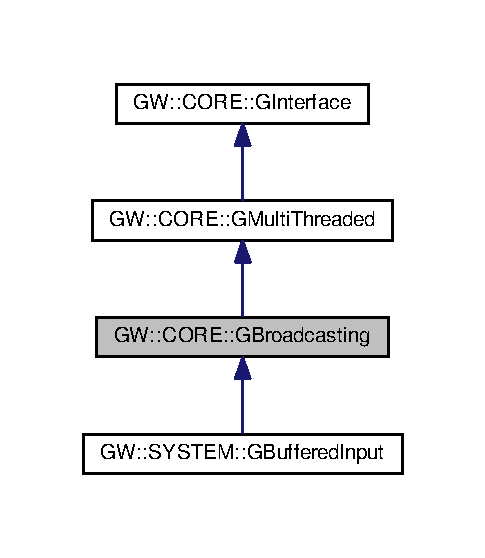
\includegraphics[width=233pt]{classGW_1_1CORE_1_1GBroadcasting__inherit__graph}
\end{center}
\end{figure}


Collaboration diagram for GW\+:\+:C\+O\+RE\+:\+:G\+Broadcasting\+:
\nopagebreak
\begin{figure}[H]
\begin{center}
\leavevmode
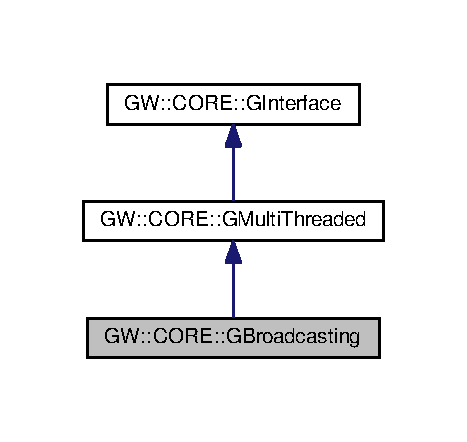
\includegraphics[width=224pt]{classGW_1_1CORE_1_1GBroadcasting__coll__graph}
\end{center}
\end{figure}
\subsection*{Public Member Functions}
\begin{DoxyCompactItemize}
\item 
virtual \hyperlink{namespaceGW_a67a839e3df7ea8a5c5686613a7a3de21}{G\+Return} \hyperlink{classGW_1_1CORE_1_1GBroadcasting_a293251421ba1169016f722df2f5b573b}{Register\+Listener} (\hyperlink{classGW_1_1CORE_1_1GListener}{G\+Listener} $\ast$\+\_\+add\+Listener, unsigned long long \+\_\+event\+Mask)=0
\begin{DoxyCompactList}\small\item\em Any listener added to this class must receive all events unless otherwise specified by the \+\_\+event\+Mask (optional). \end{DoxyCompactList}\item 
virtual \hyperlink{namespaceGW_a67a839e3df7ea8a5c5686613a7a3de21}{G\+Return} \hyperlink{classGW_1_1CORE_1_1GBroadcasting_afd6b1f41b646c668b1fcce2580681dd5}{Deregister\+Listener} (\hyperlink{classGW_1_1CORE_1_1GListener}{G\+Listener} $\ast$\+\_\+remove\+Listener)=0
\begin{DoxyCompactList}\small\item\em A successfully deregistered listener will no longer receive events and have its reference count decremented by one. \end{DoxyCompactList}\end{DoxyCompactItemize}


\subsection{Detailed Description}
The \hyperlink{classGW_1_1CORE_1_1GBroadcasting}{G\+Broadcasting} Interface is capable of registering \& deregistering \hyperlink{classGW_1_1CORE_1_1GListener}{G\+Listener} interfaces. 

The G\+Broadcaster will notify all registered listeners with the listeners On\+Event function. The events being registered for can be filtered with the \+\_\+event\+Mask (optional). 

\subsection{Member Function Documentation}
\index{G\+W\+::\+C\+O\+R\+E\+::\+G\+Broadcasting@{G\+W\+::\+C\+O\+R\+E\+::\+G\+Broadcasting}!Deregister\+Listener@{Deregister\+Listener}}
\index{Deregister\+Listener@{Deregister\+Listener}!G\+W\+::\+C\+O\+R\+E\+::\+G\+Broadcasting@{G\+W\+::\+C\+O\+R\+E\+::\+G\+Broadcasting}}
\subsubsection[{\texorpdfstring{Deregister\+Listener(\+G\+Listener $\ast$\+\_\+remove\+Listener)=0}{DeregisterListener(GListener *_removeListener)=0}}]{\setlength{\rightskip}{0pt plus 5cm}virtual {\bf G\+Return} G\+W\+::\+C\+O\+R\+E\+::\+G\+Broadcasting\+::\+Deregister\+Listener (
\begin{DoxyParamCaption}
\item[{{\bf G\+Listener} $\ast$}]{\+\_\+remove\+Listener}
\end{DoxyParamCaption}
)\hspace{0.3cm}{\ttfamily [pure virtual]}}\hypertarget{classGW_1_1CORE_1_1GBroadcasting_afd6b1f41b646c668b1fcce2580681dd5}{}\label{classGW_1_1CORE_1_1GBroadcasting_afd6b1f41b646c668b1fcce2580681dd5}


A successfully deregistered listener will no longer receive events and have its reference count decremented by one. 


\begin{DoxyParams}[1]{Parameters}
\mbox{\tt in}  & {\em \+\_\+remove\+Listener} & The listener to deregister from events.\\
\hline
\end{DoxyParams}

\begin{DoxyRetVals}{Return values}
{\em S\+U\+C\+C\+E\+SS} & The listener was successfully deregistered. \\
\hline
\end{DoxyRetVals}
\index{G\+W\+::\+C\+O\+R\+E\+::\+G\+Broadcasting@{G\+W\+::\+C\+O\+R\+E\+::\+G\+Broadcasting}!Register\+Listener@{Register\+Listener}}
\index{Register\+Listener@{Register\+Listener}!G\+W\+::\+C\+O\+R\+E\+::\+G\+Broadcasting@{G\+W\+::\+C\+O\+R\+E\+::\+G\+Broadcasting}}
\subsubsection[{\texorpdfstring{Register\+Listener(\+G\+Listener $\ast$\+\_\+add\+Listener, unsigned long long \+\_\+event\+Mask)=0}{RegisterListener(GListener *_addListener, unsigned long long _eventMask)=0}}]{\setlength{\rightskip}{0pt plus 5cm}virtual {\bf G\+Return} G\+W\+::\+C\+O\+R\+E\+::\+G\+Broadcasting\+::\+Register\+Listener (
\begin{DoxyParamCaption}
\item[{{\bf G\+Listener} $\ast$}]{\+\_\+add\+Listener, }
\item[{unsigned long long}]{\+\_\+event\+Mask}
\end{DoxyParamCaption}
)\hspace{0.3cm}{\ttfamily [pure virtual]}}\hypertarget{classGW_1_1CORE_1_1GBroadcasting_a293251421ba1169016f722df2f5b573b}{}\label{classGW_1_1CORE_1_1GBroadcasting_a293251421ba1169016f722df2f5b573b}


Any listener added to this class must receive all events unless otherwise specified by the \+\_\+event\+Mask (optional). 

Listeners registered to a broadcaster will have their reference counts increased by one until deregistered.


\begin{DoxyParams}[1]{Parameters}
\mbox{\tt in}  & {\em \+\_\+add\+Listener} & The listener object that is registering for messages. \\
\hline
\mbox{\tt in}  & {\em \+\_\+event\+Mask} & The events the listener is registering for. 0 will register for all events.\\
\hline
\end{DoxyParams}

\begin{DoxyRetVals}{Return values}
{\em S\+U\+C\+C\+E\+SS} & The listener was successfully registered. \\
\hline
{\em R\+E\+D\+U\+N\+D\+A\+N\+T\+\_\+\+O\+P\+E\+R\+A\+T\+I\+ON} & The listener has already been registered by a previous call. \\
\hline
\end{DoxyRetVals}


The documentation for this class was generated from the following file\+:\begin{DoxyCompactItemize}
\item 
Interface/\+G\+\_\+\+Core/G\+Broadcasting.\+h\end{DoxyCompactItemize}

\hypertarget{classGW_1_1SYSTEM_1_1GBufferedInput}{}\section{GW\+::S\+Y\+S\+T\+EM\+::G\+Buffered\+Input Class Reference}
\label{classGW_1_1SYSTEM_1_1GBufferedInput}\index{GW::SYSTEM::GBufferedInput@{GW::SYSTEM::GBufferedInput}}


A Multi-\/threaded buffered input library.  




{\ttfamily \#include $<$G\+Buffered\+Input.\+h$>$}



Inheritance diagram for GW\+::S\+Y\+S\+T\+EM\+::G\+Buffered\+Input\+:
% FIG 0


Collaboration diagram for GW\+::S\+Y\+S\+T\+EM\+::G\+Buffered\+Input\+:
% FIG 1
\subsection*{Additional Inherited Members}


\subsection{Detailed Description}
A Multi-\/threaded buffered input library. 

Register with a \mbox{\hyperlink{classGW_1_1SYSTEM_1_1GBufferedInput}{G\+Buffered\+Input}} to receive mouse and keyboard events. 

The documentation for this class was generated from the following file\+:\begin{DoxyCompactItemize}
\item 
Interface/\+G\+\_\+\+System/G\+Buffered\+Input.\+h\end{DoxyCompactItemize}

\hypertarget{structGW_1_1SYSTEM_1_1GBUFFEREDINPUT__EVENT__DATA}{}\section{GW\+:\+:S\+Y\+S\+T\+EM\+:\+:G\+B\+U\+F\+F\+E\+R\+E\+D\+I\+N\+P\+U\+T\+\_\+\+E\+V\+E\+N\+T\+\_\+\+D\+A\+TA Struct Reference}
\label{structGW_1_1SYSTEM_1_1GBUFFEREDINPUT__EVENT__DATA}\index{G\+W\+::\+S\+Y\+S\+T\+E\+M\+::\+G\+B\+U\+F\+F\+E\+R\+E\+D\+I\+N\+P\+U\+T\+\_\+\+E\+V\+E\+N\+T\+\_\+\+D\+A\+TA@{G\+W\+::\+S\+Y\+S\+T\+E\+M\+::\+G\+B\+U\+F\+F\+E\+R\+E\+D\+I\+N\+P\+U\+T\+\_\+\+E\+V\+E\+N\+T\+\_\+\+D\+A\+TA}}


Ensure identical binary padding for structures on all platforms.  




{\ttfamily \#include $<$G\+Buffered\+Input.\+h$>$}

\subsection*{Public Attributes}
\begin{DoxyCompactItemize}
\item 
int \hyperlink{structGW_1_1SYSTEM_1_1GBUFFEREDINPUT__EVENT__DATA_abe62d14dd92dc136e8ab4f53ee26d794}{data}
\item 
int \hyperlink{structGW_1_1SYSTEM_1_1GBUFFEREDINPUT__EVENT__DATA_a055e18b0d2aa3135ca8237bb06a0b4cb}{x}
\item 
int \hyperlink{structGW_1_1SYSTEM_1_1GBUFFEREDINPUT__EVENT__DATA_a68facd2e2754c908ecf8b8ef4ce34e08}{y}
\item 
int \hyperlink{structGW_1_1SYSTEM_1_1GBUFFEREDINPUT__EVENT__DATA_a8c87335f76992eddba30abe7312b5b43}{screenX}
\item 
int \hyperlink{structGW_1_1SYSTEM_1_1GBUFFEREDINPUT__EVENT__DATA_a066fa9b2dc654907d13590612238354d}{screenY}
\item 
unsigned int \hyperlink{structGW_1_1SYSTEM_1_1GBUFFEREDINPUT__EVENT__DATA_a7a818ba319e6693b89099938368a699e}{key\+Mask}
\end{DoxyCompactItemize}


\subsection{Detailed Description}
Ensure identical binary padding for structures on all platforms. 

\hyperlink{structGW_1_1SYSTEM_1_1GBUFFEREDINPUT__EVENT__DATA}{G\+B\+U\+F\+F\+E\+R\+E\+D\+I\+N\+P\+U\+T\+\_\+\+E\+V\+E\+N\+T\+\_\+\+D\+A\+TA} will hold any information you may need about an \hyperlink{classInput}{Input} Event. 

\subsection{Member Data Documentation}
\index{G\+W\+::\+S\+Y\+S\+T\+E\+M\+::\+G\+B\+U\+F\+F\+E\+R\+E\+D\+I\+N\+P\+U\+T\+\_\+\+E\+V\+E\+N\+T\+\_\+\+D\+A\+TA@{G\+W\+::\+S\+Y\+S\+T\+E\+M\+::\+G\+B\+U\+F\+F\+E\+R\+E\+D\+I\+N\+P\+U\+T\+\_\+\+E\+V\+E\+N\+T\+\_\+\+D\+A\+TA}!data@{data}}
\index{data@{data}!G\+W\+::\+S\+Y\+S\+T\+E\+M\+::\+G\+B\+U\+F\+F\+E\+R\+E\+D\+I\+N\+P\+U\+T\+\_\+\+E\+V\+E\+N\+T\+\_\+\+D\+A\+TA@{G\+W\+::\+S\+Y\+S\+T\+E\+M\+::\+G\+B\+U\+F\+F\+E\+R\+E\+D\+I\+N\+P\+U\+T\+\_\+\+E\+V\+E\+N\+T\+\_\+\+D\+A\+TA}}
\subsubsection[{\texorpdfstring{data}{data}}]{\setlength{\rightskip}{0pt plus 5cm}int G\+W\+::\+S\+Y\+S\+T\+E\+M\+::\+G\+B\+U\+F\+F\+E\+R\+E\+D\+I\+N\+P\+U\+T\+\_\+\+E\+V\+E\+N\+T\+\_\+\+D\+A\+T\+A\+::data}\hypertarget{structGW_1_1SYSTEM_1_1GBUFFEREDINPUT__EVENT__DATA_abe62d14dd92dc136e8ab4f53ee26d794}{}\label{structGW_1_1SYSTEM_1_1GBUFFEREDINPUT__EVENT__DATA_abe62d14dd92dc136e8ab4f53ee26d794}
Data storing the key/button information. \index{G\+W\+::\+S\+Y\+S\+T\+E\+M\+::\+G\+B\+U\+F\+F\+E\+R\+E\+D\+I\+N\+P\+U\+T\+\_\+\+E\+V\+E\+N\+T\+\_\+\+D\+A\+TA@{G\+W\+::\+S\+Y\+S\+T\+E\+M\+::\+G\+B\+U\+F\+F\+E\+R\+E\+D\+I\+N\+P\+U\+T\+\_\+\+E\+V\+E\+N\+T\+\_\+\+D\+A\+TA}!key\+Mask@{key\+Mask}}
\index{key\+Mask@{key\+Mask}!G\+W\+::\+S\+Y\+S\+T\+E\+M\+::\+G\+B\+U\+F\+F\+E\+R\+E\+D\+I\+N\+P\+U\+T\+\_\+\+E\+V\+E\+N\+T\+\_\+\+D\+A\+TA@{G\+W\+::\+S\+Y\+S\+T\+E\+M\+::\+G\+B\+U\+F\+F\+E\+R\+E\+D\+I\+N\+P\+U\+T\+\_\+\+E\+V\+E\+N\+T\+\_\+\+D\+A\+TA}}
\subsubsection[{\texorpdfstring{key\+Mask}{keyMask}}]{\setlength{\rightskip}{0pt plus 5cm}unsigned int G\+W\+::\+S\+Y\+S\+T\+E\+M\+::\+G\+B\+U\+F\+F\+E\+R\+E\+D\+I\+N\+P\+U\+T\+\_\+\+E\+V\+E\+N\+T\+\_\+\+D\+A\+T\+A\+::key\+Mask}\hypertarget{structGW_1_1SYSTEM_1_1GBUFFEREDINPUT__EVENT__DATA_a7a818ba319e6693b89099938368a699e}{}\label{structGW_1_1SYSTEM_1_1GBUFFEREDINPUT__EVENT__DATA_a7a818ba319e6693b89099938368a699e}
Bit flags for (Caps\+Lock, Num\+Lock, Scroll\+Lock, Shift, and Control). See \hyperlink{GKeyDefines_8h_source}{G\+Key\+Defines.\+h} for list of key\+Mask defines. \index{G\+W\+::\+S\+Y\+S\+T\+E\+M\+::\+G\+B\+U\+F\+F\+E\+R\+E\+D\+I\+N\+P\+U\+T\+\_\+\+E\+V\+E\+N\+T\+\_\+\+D\+A\+TA@{G\+W\+::\+S\+Y\+S\+T\+E\+M\+::\+G\+B\+U\+F\+F\+E\+R\+E\+D\+I\+N\+P\+U\+T\+\_\+\+E\+V\+E\+N\+T\+\_\+\+D\+A\+TA}!screenX@{screenX}}
\index{screenX@{screenX}!G\+W\+::\+S\+Y\+S\+T\+E\+M\+::\+G\+B\+U\+F\+F\+E\+R\+E\+D\+I\+N\+P\+U\+T\+\_\+\+E\+V\+E\+N\+T\+\_\+\+D\+A\+TA@{G\+W\+::\+S\+Y\+S\+T\+E\+M\+::\+G\+B\+U\+F\+F\+E\+R\+E\+D\+I\+N\+P\+U\+T\+\_\+\+E\+V\+E\+N\+T\+\_\+\+D\+A\+TA}}
\subsubsection[{\texorpdfstring{screenX}{screenX}}]{\setlength{\rightskip}{0pt plus 5cm}int G\+W\+::\+S\+Y\+S\+T\+E\+M\+::\+G\+B\+U\+F\+F\+E\+R\+E\+D\+I\+N\+P\+U\+T\+\_\+\+E\+V\+E\+N\+T\+\_\+\+D\+A\+T\+A\+::screenX}\hypertarget{structGW_1_1SYSTEM_1_1GBUFFEREDINPUT__EVENT__DATA_a8c87335f76992eddba30abe7312b5b43}{}\label{structGW_1_1SYSTEM_1_1GBUFFEREDINPUT__EVENT__DATA_a8c87335f76992eddba30abe7312b5b43}
Screen Mouse position x when event is sent. \index{G\+W\+::\+S\+Y\+S\+T\+E\+M\+::\+G\+B\+U\+F\+F\+E\+R\+E\+D\+I\+N\+P\+U\+T\+\_\+\+E\+V\+E\+N\+T\+\_\+\+D\+A\+TA@{G\+W\+::\+S\+Y\+S\+T\+E\+M\+::\+G\+B\+U\+F\+F\+E\+R\+E\+D\+I\+N\+P\+U\+T\+\_\+\+E\+V\+E\+N\+T\+\_\+\+D\+A\+TA}!screenY@{screenY}}
\index{screenY@{screenY}!G\+W\+::\+S\+Y\+S\+T\+E\+M\+::\+G\+B\+U\+F\+F\+E\+R\+E\+D\+I\+N\+P\+U\+T\+\_\+\+E\+V\+E\+N\+T\+\_\+\+D\+A\+TA@{G\+W\+::\+S\+Y\+S\+T\+E\+M\+::\+G\+B\+U\+F\+F\+E\+R\+E\+D\+I\+N\+P\+U\+T\+\_\+\+E\+V\+E\+N\+T\+\_\+\+D\+A\+TA}}
\subsubsection[{\texorpdfstring{screenY}{screenY}}]{\setlength{\rightskip}{0pt plus 5cm}int G\+W\+::\+S\+Y\+S\+T\+E\+M\+::\+G\+B\+U\+F\+F\+E\+R\+E\+D\+I\+N\+P\+U\+T\+\_\+\+E\+V\+E\+N\+T\+\_\+\+D\+A\+T\+A\+::screenY}\hypertarget{structGW_1_1SYSTEM_1_1GBUFFEREDINPUT__EVENT__DATA_a066fa9b2dc654907d13590612238354d}{}\label{structGW_1_1SYSTEM_1_1GBUFFEREDINPUT__EVENT__DATA_a066fa9b2dc654907d13590612238354d}
Screen Mouse position y when event is sent. \index{G\+W\+::\+S\+Y\+S\+T\+E\+M\+::\+G\+B\+U\+F\+F\+E\+R\+E\+D\+I\+N\+P\+U\+T\+\_\+\+E\+V\+E\+N\+T\+\_\+\+D\+A\+TA@{G\+W\+::\+S\+Y\+S\+T\+E\+M\+::\+G\+B\+U\+F\+F\+E\+R\+E\+D\+I\+N\+P\+U\+T\+\_\+\+E\+V\+E\+N\+T\+\_\+\+D\+A\+TA}!x@{x}}
\index{x@{x}!G\+W\+::\+S\+Y\+S\+T\+E\+M\+::\+G\+B\+U\+F\+F\+E\+R\+E\+D\+I\+N\+P\+U\+T\+\_\+\+E\+V\+E\+N\+T\+\_\+\+D\+A\+TA@{G\+W\+::\+S\+Y\+S\+T\+E\+M\+::\+G\+B\+U\+F\+F\+E\+R\+E\+D\+I\+N\+P\+U\+T\+\_\+\+E\+V\+E\+N\+T\+\_\+\+D\+A\+TA}}
\subsubsection[{\texorpdfstring{x}{x}}]{\setlength{\rightskip}{0pt plus 5cm}int G\+W\+::\+S\+Y\+S\+T\+E\+M\+::\+G\+B\+U\+F\+F\+E\+R\+E\+D\+I\+N\+P\+U\+T\+\_\+\+E\+V\+E\+N\+T\+\_\+\+D\+A\+T\+A\+::x}\hypertarget{structGW_1_1SYSTEM_1_1GBUFFEREDINPUT__EVENT__DATA_a055e18b0d2aa3135ca8237bb06a0b4cb}{}\label{structGW_1_1SYSTEM_1_1GBUFFEREDINPUT__EVENT__DATA_a055e18b0d2aa3135ca8237bb06a0b4cb}
Window Mouse position x when event is sent. \index{G\+W\+::\+S\+Y\+S\+T\+E\+M\+::\+G\+B\+U\+F\+F\+E\+R\+E\+D\+I\+N\+P\+U\+T\+\_\+\+E\+V\+E\+N\+T\+\_\+\+D\+A\+TA@{G\+W\+::\+S\+Y\+S\+T\+E\+M\+::\+G\+B\+U\+F\+F\+E\+R\+E\+D\+I\+N\+P\+U\+T\+\_\+\+E\+V\+E\+N\+T\+\_\+\+D\+A\+TA}!y@{y}}
\index{y@{y}!G\+W\+::\+S\+Y\+S\+T\+E\+M\+::\+G\+B\+U\+F\+F\+E\+R\+E\+D\+I\+N\+P\+U\+T\+\_\+\+E\+V\+E\+N\+T\+\_\+\+D\+A\+TA@{G\+W\+::\+S\+Y\+S\+T\+E\+M\+::\+G\+B\+U\+F\+F\+E\+R\+E\+D\+I\+N\+P\+U\+T\+\_\+\+E\+V\+E\+N\+T\+\_\+\+D\+A\+TA}}
\subsubsection[{\texorpdfstring{y}{y}}]{\setlength{\rightskip}{0pt plus 5cm}int G\+W\+::\+S\+Y\+S\+T\+E\+M\+::\+G\+B\+U\+F\+F\+E\+R\+E\+D\+I\+N\+P\+U\+T\+\_\+\+E\+V\+E\+N\+T\+\_\+\+D\+A\+T\+A\+::y}\hypertarget{structGW_1_1SYSTEM_1_1GBUFFEREDINPUT__EVENT__DATA_a68facd2e2754c908ecf8b8ef4ce34e08}{}\label{structGW_1_1SYSTEM_1_1GBUFFEREDINPUT__EVENT__DATA_a68facd2e2754c908ecf8b8ef4ce34e08}
Window Mouse position y when event is sent. 

The documentation for this struct was generated from the following file\+:\begin{DoxyCompactItemize}
\item 
Interface/\+G\+\_\+\+System/G\+Buffered\+Input.\+h\end{DoxyCompactItemize}

\hypertarget{classGBufferedInputTestListener}{}\section{G\+Buffered\+Input\+Test\+Listener Class Reference}
\label{classGBufferedInputTestListener}\index{G\+Buffered\+Input\+Test\+Listener@{G\+Buffered\+Input\+Test\+Listener}}


Inheritance diagram for G\+Buffered\+Input\+Test\+Listener\+:
\nopagebreak
\begin{figure}[H]
\begin{center}
\leavevmode
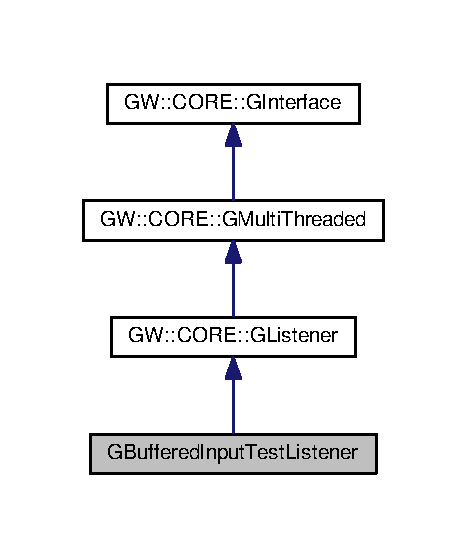
\includegraphics[width=224pt]{classGBufferedInputTestListener__inherit__graph}
\end{center}
\end{figure}


Collaboration diagram for G\+Buffered\+Input\+Test\+Listener\+:
\nopagebreak
\begin{figure}[H]
\begin{center}
\leavevmode
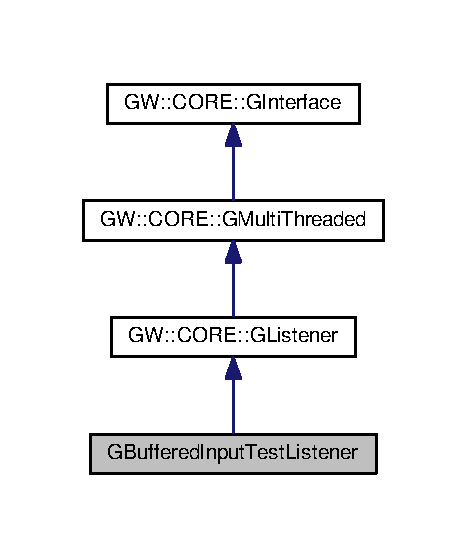
\includegraphics[width=224pt]{classGBufferedInputTestListener__coll__graph}
\end{center}
\end{figure}
\subsection*{Public Member Functions}
\begin{DoxyCompactItemize}
\item 
\hyperlink{namespaceGW_a67a839e3df7ea8a5c5686613a7a3de21}{G\+W\+::\+G\+Return} \hyperlink{classGBufferedInputTestListener_a72ad4efa12481df3cb87de61a58c0903}{On\+Event} (const \hyperlink{structGW_1_1GUUIID}{G\+W\+::\+G\+U\+U\+I\+ID} \&\+\_\+sender\+Interface, unsigned int \+\_\+event\+ID, void $\ast$\+\_\+event\+Data, unsigned int \+\_\+size\+Of\+Data)
\begin{DoxyCompactList}\small\item\em This operation is called whenever a G\+Broadcaster a listener is registered to generates an event. \end{DoxyCompactList}\item 
\hyperlink{namespaceGW_a67a839e3df7ea8a5c5686613a7a3de21}{G\+W\+::\+G\+Return} \hyperlink{classGBufferedInputTestListener_a91b6ab9254bc3886b42ca021ff6b4acd}{Get\+Count} (unsigned int \&\+\_\+out\+Count)
\begin{DoxyCompactList}\small\item\em Return the total number of active references to this object. \end{DoxyCompactList}\item 
\hyperlink{namespaceGW_a67a839e3df7ea8a5c5686613a7a3de21}{G\+W\+::\+G\+Return} \hyperlink{classGBufferedInputTestListener_af3a9ea97e6ab7d5350a4090aae43c471}{Increment\+Count} ()
\begin{DoxyCompactList}\small\item\em Increase the total number of active references to this object. \end{DoxyCompactList}\item 
\hyperlink{namespaceGW_a67a839e3df7ea8a5c5686613a7a3de21}{G\+W\+::\+G\+Return} \hyperlink{classGBufferedInputTestListener_a283260f6f72cfcbcc4e65c1e0635f789}{Decrement\+Count} ()
\begin{DoxyCompactList}\small\item\em Decrease the total number of active references to this object. \end{DoxyCompactList}\item 
\hyperlink{namespaceGW_a67a839e3df7ea8a5c5686613a7a3de21}{G\+W\+::\+G\+Return} \hyperlink{classGBufferedInputTestListener_ad3ed9fa46132f9b81651af2fde31eee6}{Request\+Interface} (const \hyperlink{structGW_1_1GUUIID}{G\+W\+::\+G\+U\+U\+I\+ID} \&\+\_\+interface\+ID, void $\ast$$\ast$\+\_\+output\+Interface)
\begin{DoxyCompactList}\small\item\em Requests an interface that may or may not be supported by this object. \end{DoxyCompactList}\end{DoxyCompactItemize}


\subsection{Member Function Documentation}
\index{G\+Buffered\+Input\+Test\+Listener@{G\+Buffered\+Input\+Test\+Listener}!Decrement\+Count@{Decrement\+Count}}
\index{Decrement\+Count@{Decrement\+Count}!G\+Buffered\+Input\+Test\+Listener@{G\+Buffered\+Input\+Test\+Listener}}
\subsubsection[{\texorpdfstring{Decrement\+Count()}{DecrementCount()}}]{\setlength{\rightskip}{0pt plus 5cm}{\bf G\+W\+::\+G\+Return} G\+Buffered\+Input\+Test\+Listener\+::\+Decrement\+Count (
\begin{DoxyParamCaption}
{}
\end{DoxyParamCaption}
)\hspace{0.3cm}{\ttfamily [virtual]}}\hypertarget{classGBufferedInputTestListener_a283260f6f72cfcbcc4e65c1e0635f789}{}\label{classGBufferedInputTestListener_a283260f6f72cfcbcc4e65c1e0635f789}


Decrease the total number of active references to this object. 

Once the internal count reaches zero this object will be deallocated and your pointer will become invalid.


\begin{DoxyRetVals}{Return values}
{\em S\+U\+C\+C\+E\+SS} & Successfully decremented the internal reference count. \\
\hline
{\em F\+A\+I\+L\+U\+RE} & Decrementing of internal reference count would underflow the value. \\
\hline
\end{DoxyRetVals}


Implements \hyperlink{classGW_1_1CORE_1_1GInterface_a19a368c77ad0aa7f49b5a4f772f173ba}{G\+W\+::\+C\+O\+R\+E\+::\+G\+Interface}.

\index{G\+Buffered\+Input\+Test\+Listener@{G\+Buffered\+Input\+Test\+Listener}!Get\+Count@{Get\+Count}}
\index{Get\+Count@{Get\+Count}!G\+Buffered\+Input\+Test\+Listener@{G\+Buffered\+Input\+Test\+Listener}}
\subsubsection[{\texorpdfstring{Get\+Count(unsigned int \&\+\_\+out\+Count)}{GetCount(unsigned int &_outCount)}}]{\setlength{\rightskip}{0pt plus 5cm}{\bf G\+W\+::\+G\+Return} G\+Buffered\+Input\+Test\+Listener\+::\+Get\+Count (
\begin{DoxyParamCaption}
\item[{unsigned int \&}]{\+\_\+out\+Count}
\end{DoxyParamCaption}
)\hspace{0.3cm}{\ttfamily [virtual]}}\hypertarget{classGBufferedInputTestListener_a91b6ab9254bc3886b42ca021ff6b4acd}{}\label{classGBufferedInputTestListener_a91b6ab9254bc3886b42ca021ff6b4acd}


Return the total number of active references to this object. 


\begin{DoxyParams}[1]{Parameters}
\mbox{\tt out}  & {\em \+\_\+out\+Count} & The total number of active references of this object.\\
\hline
\end{DoxyParams}

\begin{DoxyRetVals}{Return values}
{\em S\+U\+C\+C\+E\+SS} & Successfully ran. \\
\hline
{\em F\+A\+I\+L\+U\+RE} & Either class does not exist or the internal reference count is corrupt. \\
\hline
\end{DoxyRetVals}


Implements \hyperlink{classGW_1_1CORE_1_1GInterface_aacf5834174a7024f8a3c361122ee9e76}{G\+W\+::\+C\+O\+R\+E\+::\+G\+Interface}.

\index{G\+Buffered\+Input\+Test\+Listener@{G\+Buffered\+Input\+Test\+Listener}!Increment\+Count@{Increment\+Count}}
\index{Increment\+Count@{Increment\+Count}!G\+Buffered\+Input\+Test\+Listener@{G\+Buffered\+Input\+Test\+Listener}}
\subsubsection[{\texorpdfstring{Increment\+Count()}{IncrementCount()}}]{\setlength{\rightskip}{0pt plus 5cm}{\bf G\+W\+::\+G\+Return} G\+Buffered\+Input\+Test\+Listener\+::\+Increment\+Count (
\begin{DoxyParamCaption}
{}
\end{DoxyParamCaption}
)\hspace{0.3cm}{\ttfamily [virtual]}}\hypertarget{classGBufferedInputTestListener_af3a9ea97e6ab7d5350a4090aae43c471}{}\label{classGBufferedInputTestListener_af3a9ea97e6ab7d5350a4090aae43c471}


Increase the total number of active references to this object. 

End users should only call this operation if they are familiar with reference counting behavior.


\begin{DoxyRetVals}{Return values}
{\em S\+U\+C\+C\+E\+SS} & Successfully incremented the internal reference count. \\
\hline
{\em F\+A\+I\+L\+U\+RE} & Incrementation of internal reference count would overflow the value. \\
\hline
\end{DoxyRetVals}


Implements \hyperlink{classGW_1_1CORE_1_1GInterface_a2d710f20bb78e544e8309b5b75c21260}{G\+W\+::\+C\+O\+R\+E\+::\+G\+Interface}.

\index{G\+Buffered\+Input\+Test\+Listener@{G\+Buffered\+Input\+Test\+Listener}!On\+Event@{On\+Event}}
\index{On\+Event@{On\+Event}!G\+Buffered\+Input\+Test\+Listener@{G\+Buffered\+Input\+Test\+Listener}}
\subsubsection[{\texorpdfstring{On\+Event(const G\+W\+::\+G\+U\+U\+I\+I\+D \&\+\_\+sender\+Interface, unsigned int \+\_\+event\+I\+D, void $\ast$\+\_\+event\+Data, unsigned int \+\_\+size\+Of\+Data)}{OnEvent(const GW::GUUIID &_senderInterface, unsigned int _eventID, void *_eventData, unsigned int _sizeOfData)}}]{\setlength{\rightskip}{0pt plus 5cm}{\bf G\+W\+::\+G\+Return} G\+Buffered\+Input\+Test\+Listener\+::\+On\+Event (
\begin{DoxyParamCaption}
\item[{const {\bf G\+W\+::\+G\+U\+U\+I\+ID} \&}]{\+\_\+sender\+Interface, }
\item[{unsigned int}]{\+\_\+event\+ID, }
\item[{void $\ast$}]{\+\_\+event\+Data, }
\item[{unsigned int}]{\+\_\+data\+Size}
\end{DoxyParamCaption}
)\hspace{0.3cm}{\ttfamily [virtual]}}\hypertarget{classGBufferedInputTestListener_a72ad4efa12481df3cb87de61a58c0903}{}\label{classGBufferedInputTestListener_a72ad4efa12481df3cb87de61a58c0903}


This operation is called whenever a G\+Broadcaster a listener is registered to generates an event. 


\begin{DoxyParams}[1]{Parameters}
\mbox{\tt in}  & {\em \+\_\+sender\+Interface} & The interface of the sender object. \\
\hline
\mbox{\tt in}  & {\em \+\_\+event\+ID} & The ID of the event sent. \\
\hline
\mbox{\tt in}  & {\em \+\_\+event\+Data} & The data of the event. \\
\hline
\mbox{\tt in}  & {\em \+\_\+data\+Size} & The size of \+\_\+event\+Data in bytes. \\
\hline
\end{DoxyParams}


Implements \hyperlink{classGW_1_1CORE_1_1GListener_a5c1d1fac213b7a1cc15d384aa0c33105}{G\+W\+::\+C\+O\+R\+E\+::\+G\+Listener}.

\index{G\+Buffered\+Input\+Test\+Listener@{G\+Buffered\+Input\+Test\+Listener}!Request\+Interface@{Request\+Interface}}
\index{Request\+Interface@{Request\+Interface}!G\+Buffered\+Input\+Test\+Listener@{G\+Buffered\+Input\+Test\+Listener}}
\subsubsection[{\texorpdfstring{Request\+Interface(const G\+W\+::\+G\+U\+U\+I\+I\+D \&\+\_\+interface\+I\+D, void $\ast$$\ast$\+\_\+output\+Interface)}{RequestInterface(const GW::GUUIID &_interfaceID, void **_outputInterface)}}]{\setlength{\rightskip}{0pt plus 5cm}{\bf G\+W\+::\+G\+Return} G\+Buffered\+Input\+Test\+Listener\+::\+Request\+Interface (
\begin{DoxyParamCaption}
\item[{const {\bf G\+W\+::\+G\+U\+U\+I\+ID} \&}]{\+\_\+interface\+ID, }
\item[{void $\ast$$\ast$}]{\+\_\+output\+Interface}
\end{DoxyParamCaption}
)\hspace{0.3cm}{\ttfamily [virtual]}}\hypertarget{classGBufferedInputTestListener_ad3ed9fa46132f9b81651af2fde31eee6}{}\label{classGBufferedInputTestListener_ad3ed9fa46132f9b81651af2fde31eee6}


Requests an interface that may or may not be supported by this object. 

Can be used by the end-\/user to query for a new interface using the unique ID of the interface they want and implement an interface update.


\begin{DoxyParams}[1]{Parameters}
\mbox{\tt in}  & {\em \+\_\+interface\+ID} & The G\+U\+U\+I\+ID of the interface you are requesting. \\
\hline
\mbox{\tt out}  & {\em \+\_\+output\+Interface} & Where the interface will be stored if function is successful.\\
\hline
\end{DoxyParams}

\begin{DoxyRetVals}{Return values}
{\em S\+U\+C\+C\+E\+SS} & The interface is supported and function succeded. \\
\hline
{\em I\+N\+T\+E\+R\+F\+A\+C\+E\+\_\+\+U\+N\+S\+U\+P\+P\+O\+R\+T\+ED} & The requested interface is not supported. \\
\hline
\end{DoxyRetVals}


Implements \hyperlink{classGW_1_1CORE_1_1GInterface_ad6c8324970172784964f484686d4fdad}{G\+W\+::\+C\+O\+R\+E\+::\+G\+Interface}.



The documentation for this class was generated from the following files\+:\begin{DoxyCompactItemize}
\item 
Unit Tests/\+G\+\_\+\+System/G\+Buffered\+Input\+Test\+Listener.\+h\item 
Unit Tests/\+G\+\_\+\+System/G\+Buffered\+Input\+Test\+Listener.\+cpp\end{DoxyCompactItemize}

\hypertarget{classGW_1_1SYSTEM_1_1GFile}{}\section{GW\+:\+:S\+Y\+S\+T\+EM\+:\+:G\+File Class Reference}
\label{classGW_1_1SYSTEM_1_1GFile}\index{G\+W\+::\+S\+Y\+S\+T\+E\+M\+::\+G\+File@{G\+W\+::\+S\+Y\+S\+T\+E\+M\+::\+G\+File}}


Cross platform File\+I\+O/\+Directory handling.  




{\ttfamily \#include $<$G\+File.\+h$>$}



Inheritance diagram for GW\+:\+:S\+Y\+S\+T\+EM\+:\+:G\+File\+:
\nopagebreak
\begin{figure}[H]
\begin{center}
\leavevmode
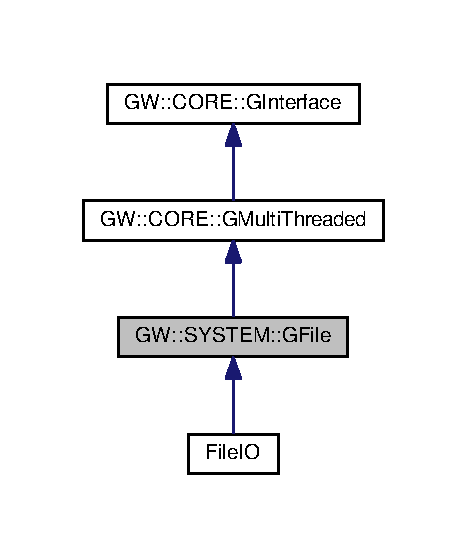
\includegraphics[width=224pt]{classGW_1_1SYSTEM_1_1GFile__inherit__graph}
\end{center}
\end{figure}


Collaboration diagram for GW\+:\+:S\+Y\+S\+T\+EM\+:\+:G\+File\+:
\nopagebreak
\begin{figure}[H]
\begin{center}
\leavevmode
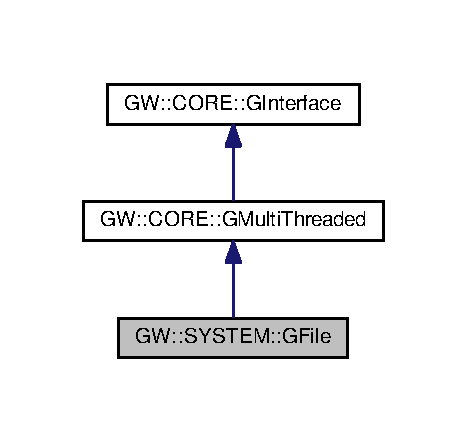
\includegraphics[width=224pt]{classGW_1_1SYSTEM_1_1GFile__coll__graph}
\end{center}
\end{figure}
\subsection*{Public Member Functions}
\begin{DoxyCompactItemize}
\item 
virtual \hyperlink{namespaceGW_a67a839e3df7ea8a5c5686613a7a3de21}{G\+Return} \hyperlink{classGW_1_1SYSTEM_1_1GFile_a2744359d5d258b1b59d139101c6809ce}{Open\+Binary\+Read} (const char $\ast$const \+\_\+file)=0
\begin{DoxyCompactList}\small\item\em Opens a file for binary read. \end{DoxyCompactList}\item 
virtual \hyperlink{namespaceGW_a67a839e3df7ea8a5c5686613a7a3de21}{G\+Return} \hyperlink{classGW_1_1SYSTEM_1_1GFile_a8d5f335bbc6f7c6d798ed27718aa2347}{Open\+Binary\+Write} (const char $\ast$const \+\_\+file)=0
\begin{DoxyCompactList}\small\item\em Opens a file for binary write with truncation. \end{DoxyCompactList}\item 
virtual \hyperlink{namespaceGW_a67a839e3df7ea8a5c5686613a7a3de21}{G\+Return} \hyperlink{classGW_1_1SYSTEM_1_1GFile_a63311236692181f99fd393fe8e1ca9fc}{Append\+Binary\+Write} (const char $\ast$const \+\_\+file)=0
\begin{DoxyCompactList}\small\item\em Opens a file for binary write with append. \end{DoxyCompactList}\item 
virtual \hyperlink{namespaceGW_a67a839e3df7ea8a5c5686613a7a3de21}{G\+Return} \hyperlink{classGW_1_1SYSTEM_1_1GFile_ac3ece72ce30e4d1a1c426c53a7a8354a}{Open\+Text\+Read} (const char $\ast$const \+\_\+file)=0
\begin{DoxyCompactList}\small\item\em Opens a file for text read. \end{DoxyCompactList}\item 
virtual \hyperlink{namespaceGW_a67a839e3df7ea8a5c5686613a7a3de21}{G\+Return} \hyperlink{classGW_1_1SYSTEM_1_1GFile_aebd3e32736b994c0296b7575ab0a2759}{Open\+Text\+Write} (const char $\ast$const \+\_\+file)=0
\begin{DoxyCompactList}\small\item\em Opens a file for text write with truncation. \end{DoxyCompactList}\item 
virtual \hyperlink{namespaceGW_a67a839e3df7ea8a5c5686613a7a3de21}{G\+Return} \hyperlink{classGW_1_1SYSTEM_1_1GFile_a72e40b3234a2384738d8db6e958f4782}{Append\+Text\+Write} (const char $\ast$const \+\_\+file)=0
\begin{DoxyCompactList}\small\item\em Opens a file for text write with append. \end{DoxyCompactList}\item 
virtual \hyperlink{namespaceGW_a67a839e3df7ea8a5c5686613a7a3de21}{G\+Return} \hyperlink{classGW_1_1SYSTEM_1_1GFile_ae9906414c159e9f1156b5ff6ad511c31}{Write} (const char $\ast$const \+\_\+in\+Data, unsigned int \+\_\+num\+Bytes)=0
\begin{DoxyCompactList}\small\item\em Writes binary data to the currently opened file. \end{DoxyCompactList}\item 
virtual \hyperlink{namespaceGW_a67a839e3df7ea8a5c5686613a7a3de21}{G\+Return} \hyperlink{classGW_1_1SYSTEM_1_1GFile_a1aaa026cba3d37abaaa2b408cd5d322d}{Read} (char $\ast$\+\_\+out\+Data, unsigned int \+\_\+num\+Bytes)=0
\begin{DoxyCompactList}\small\item\em Reads binary from the currently opened file. \end{DoxyCompactList}\item 
virtual \hyperlink{namespaceGW_a67a839e3df7ea8a5c5686613a7a3de21}{G\+Return} \hyperlink{classGW_1_1SYSTEM_1_1GFile_a7c57570575c63ae98f71232660d1b911}{Write\+Line} (const char $\ast$const \+\_\+in\+Data)=0
\begin{DoxyCompactList}\small\item\em Writes text to the currently opened file. \end{DoxyCompactList}\item 
virtual \hyperlink{namespaceGW_a67a839e3df7ea8a5c5686613a7a3de21}{G\+Return} \hyperlink{classGW_1_1SYSTEM_1_1GFile_ae9e072091ffe55f2f7697cb1d3eaec79}{Read\+Line} (char $\ast$\+\_\+out\+Data, unsigned int \+\_\+out\+Data\+Size, char \+\_\+delimiter)=0
\begin{DoxyCompactList}\small\item\em Reads text to the currently opened file. \end{DoxyCompactList}\item 
virtual \hyperlink{namespaceGW_a67a839e3df7ea8a5c5686613a7a3de21}{G\+Return} \hyperlink{classGW_1_1SYSTEM_1_1GFile_ae661d107c461145bb095dcfc76519f54}{Close\+File} ()=0
\begin{DoxyCompactList}\small\item\em Flushes and closes the current file. \end{DoxyCompactList}\item 
virtual \hyperlink{namespaceGW_a67a839e3df7ea8a5c5686613a7a3de21}{G\+Return} \hyperlink{classGW_1_1SYSTEM_1_1GFile_ae3105b637ef87af268722a696b8657a9}{Flush\+File} ()=0
\begin{DoxyCompactList}\small\item\em Flushes the current file. \end{DoxyCompactList}\item 
virtual \hyperlink{namespaceGW_a67a839e3df7ea8a5c5686613a7a3de21}{G\+Return} \hyperlink{classGW_1_1SYSTEM_1_1GFile_ab28d2e7ecf3ac893df88603e5448561a}{Set\+Current\+Working\+Directory} (const char $\ast$const \+\_\+dir)=0
\begin{DoxyCompactList}\small\item\em Changes the current working directory. \end{DoxyCompactList}\item 
virtual \hyperlink{namespaceGW_a67a839e3df7ea8a5c5686613a7a3de21}{G\+Return} \hyperlink{classGW_1_1SYSTEM_1_1GFile_a6853b717e838d1b3a54f22449a37d764}{Get\+Current\+Working\+Directory} (char $\ast$\+\_\+out\+Dir, unsigned int \+\_\+dir\+Size)=0
\begin{DoxyCompactList}\small\item\em Retrieves the absolute path of the current working directory. \end{DoxyCompactList}\item 
virtual \hyperlink{namespaceGW_a67a839e3df7ea8a5c5686613a7a3de21}{G\+Return} \hyperlink{classGW_1_1SYSTEM_1_1GFile_ac2de86bf6cf61455577efc47277ecb94}{Get\+Directory\+Size} (unsigned int \&\+\_\+out\+Size)=0
\begin{DoxyCompactList}\small\item\em Gets the number of files in the current working directory. \end{DoxyCompactList}\item 
virtual \hyperlink{namespaceGW_a67a839e3df7ea8a5c5686613a7a3de21}{G\+Return} \hyperlink{classGW_1_1SYSTEM_1_1GFile_ae062d19f84d120adea94756d1d26e41e}{Get\+Files\+From\+Directory} (char $\ast$\+\_\+out\+Files\mbox{[}$\,$\mbox{]}, unsigned int \+\_\+num\+Files, unsigned int \+\_\+file\+Name\+Size)=0
\begin{DoxyCompactList}\small\item\em Gets the names of all files in the current working directory. \end{DoxyCompactList}\item 
virtual \hyperlink{namespaceGW_a67a839e3df7ea8a5c5686613a7a3de21}{G\+Return} \hyperlink{classGW_1_1SYSTEM_1_1GFile_a2f4cba2dad96fa4c894545f43fee64b5}{Get\+File\+Size} (const char $\ast$const \+\_\+file, unsigned int \&\+\_\+out\+Size)=0
\begin{DoxyCompactList}\small\item\em Gets the size of the specified file in bytes. \end{DoxyCompactList}\end{DoxyCompactItemize}


\subsection{Detailed Description}
Cross platform File\+I\+O/\+Directory handling. 

Handles file input/output operations, as well as directory information and file information. Inherits from G\+Multi\+Threaded, therfore its implementation must be thread safe. 

\subsection{Member Function Documentation}
\index{G\+W\+::\+S\+Y\+S\+T\+E\+M\+::\+G\+File@{G\+W\+::\+S\+Y\+S\+T\+E\+M\+::\+G\+File}!Append\+Binary\+Write@{Append\+Binary\+Write}}
\index{Append\+Binary\+Write@{Append\+Binary\+Write}!G\+W\+::\+S\+Y\+S\+T\+E\+M\+::\+G\+File@{G\+W\+::\+S\+Y\+S\+T\+E\+M\+::\+G\+File}}
\subsubsection[{\texorpdfstring{Append\+Binary\+Write(const char $\ast$const \+\_\+file)=0}{AppendBinaryWrite(const char *const _file)=0}}]{\setlength{\rightskip}{0pt plus 5cm}virtual {\bf G\+Return} G\+W\+::\+S\+Y\+S\+T\+E\+M\+::\+G\+File\+::\+Append\+Binary\+Write (
\begin{DoxyParamCaption}
\item[{const char $\ast$const}]{\+\_\+file}
\end{DoxyParamCaption}
)\hspace{0.3cm}{\ttfamily [pure virtual]}}\hypertarget{classGW_1_1SYSTEM_1_1GFile_a63311236692181f99fd393fe8e1ca9fc}{}\label{classGW_1_1SYSTEM_1_1GFile_a63311236692181f99fd393fe8e1ca9fc}


Opens a file for binary write with append. 

The file name passed into the function should be passed like it is a relative path. The function will look in the current working directory for the file. If the file is not found in the current working directory, the file will be created in the current working directory. File can now be written to with \hyperlink{classGW_1_1SYSTEM_1_1GFile_ae9906414c159e9f1156b5ff6ad511c31}{Write()}.


\begin{DoxyParams}[1]{Parameters}
\mbox{\tt in}  & {\em \+\_\+file} & The file name of the file to open.\\
\hline
\end{DoxyParams}

\begin{DoxyRetVals}{Return values}
{\em S\+U\+C\+C\+E\+SS} & Succesfully opened the file. \\
\hline
{\em F\+A\+I\+L\+U\+RE} & A file is already open or the file could not be found/created. \\
\hline
{\em I\+N\+V\+A\+L\+I\+D\+\_\+\+A\+R\+G\+U\+M\+E\+NT} & A nullptr was passed in. \\
\hline
\end{DoxyRetVals}


Implemented in \hyperlink{classFileIO_ab26fc846b30446edf28ac922759c9e5e}{File\+IO}.

\index{G\+W\+::\+S\+Y\+S\+T\+E\+M\+::\+G\+File@{G\+W\+::\+S\+Y\+S\+T\+E\+M\+::\+G\+File}!Append\+Text\+Write@{Append\+Text\+Write}}
\index{Append\+Text\+Write@{Append\+Text\+Write}!G\+W\+::\+S\+Y\+S\+T\+E\+M\+::\+G\+File@{G\+W\+::\+S\+Y\+S\+T\+E\+M\+::\+G\+File}}
\subsubsection[{\texorpdfstring{Append\+Text\+Write(const char $\ast$const \+\_\+file)=0}{AppendTextWrite(const char *const _file)=0}}]{\setlength{\rightskip}{0pt plus 5cm}virtual {\bf G\+Return} G\+W\+::\+S\+Y\+S\+T\+E\+M\+::\+G\+File\+::\+Append\+Text\+Write (
\begin{DoxyParamCaption}
\item[{const char $\ast$const}]{\+\_\+file}
\end{DoxyParamCaption}
)\hspace{0.3cm}{\ttfamily [pure virtual]}}\hypertarget{classGW_1_1SYSTEM_1_1GFile_a72e40b3234a2384738d8db6e958f4782}{}\label{classGW_1_1SYSTEM_1_1GFile_a72e40b3234a2384738d8db6e958f4782}


Opens a file for text write with append. 

The file name passed into the function should be passed like it is a relative path. The function will look in the current working directory for the file. If the file is not found in the current working directory, the file will be created in the current working directory. File can now be written to with \hyperlink{classGW_1_1SYSTEM_1_1GFile_ae9906414c159e9f1156b5ff6ad511c31}{Write()}.


\begin{DoxyParams}[1]{Parameters}
\mbox{\tt in}  & {\em \+\_\+file} & The file name of the file to open.\\
\hline
\end{DoxyParams}

\begin{DoxyRetVals}{Return values}
{\em S\+U\+C\+C\+E\+SS} & Succesfully opened the file. \\
\hline
{\em F\+A\+I\+L\+U\+RE} & A file is already open or the file could not be found/created. \\
\hline
{\em I\+N\+V\+A\+L\+I\+D\+\_\+\+A\+R\+G\+U\+M\+E\+NT} & A nullptr was passed in. \\
\hline
\end{DoxyRetVals}


Implemented in \hyperlink{classFileIO_afd4e0d14b85d8c0aded66bd946c291f4}{File\+IO}.

\index{G\+W\+::\+S\+Y\+S\+T\+E\+M\+::\+G\+File@{G\+W\+::\+S\+Y\+S\+T\+E\+M\+::\+G\+File}!Close\+File@{Close\+File}}
\index{Close\+File@{Close\+File}!G\+W\+::\+S\+Y\+S\+T\+E\+M\+::\+G\+File@{G\+W\+::\+S\+Y\+S\+T\+E\+M\+::\+G\+File}}
\subsubsection[{\texorpdfstring{Close\+File()=0}{CloseFile()=0}}]{\setlength{\rightskip}{0pt plus 5cm}virtual {\bf G\+Return} G\+W\+::\+S\+Y\+S\+T\+E\+M\+::\+G\+File\+::\+Close\+File (
\begin{DoxyParamCaption}
{}
\end{DoxyParamCaption}
)\hspace{0.3cm}{\ttfamily [pure virtual]}}\hypertarget{classGW_1_1SYSTEM_1_1GFile_ae661d107c461145bb095dcfc76519f54}{}\label{classGW_1_1SYSTEM_1_1GFile_ae661d107c461145bb095dcfc76519f54}


Flushes and closes the current file. 


\begin{DoxyRetVals}{Return values}
{\em S\+U\+C\+C\+E\+SS} & File successfully flushed and closed. \\
\hline
{\em F\+A\+I\+L\+U\+RE} & A file is not currently open. \\
\hline
\end{DoxyRetVals}


Implemented in \hyperlink{classFileIO_a906610c8653ba8ca476dc46679851590}{File\+IO}.

\index{G\+W\+::\+S\+Y\+S\+T\+E\+M\+::\+G\+File@{G\+W\+::\+S\+Y\+S\+T\+E\+M\+::\+G\+File}!Flush\+File@{Flush\+File}}
\index{Flush\+File@{Flush\+File}!G\+W\+::\+S\+Y\+S\+T\+E\+M\+::\+G\+File@{G\+W\+::\+S\+Y\+S\+T\+E\+M\+::\+G\+File}}
\subsubsection[{\texorpdfstring{Flush\+File()=0}{FlushFile()=0}}]{\setlength{\rightskip}{0pt plus 5cm}virtual {\bf G\+Return} G\+W\+::\+S\+Y\+S\+T\+E\+M\+::\+G\+File\+::\+Flush\+File (
\begin{DoxyParamCaption}
{}
\end{DoxyParamCaption}
)\hspace{0.3cm}{\ttfamily [pure virtual]}}\hypertarget{classGW_1_1SYSTEM_1_1GFile_ae3105b637ef87af268722a696b8657a9}{}\label{classGW_1_1SYSTEM_1_1GFile_ae3105b637ef87af268722a696b8657a9}


Flushes the current file. 


\begin{DoxyRetVals}{Return values}
{\em S\+U\+C\+C\+E\+SS} & File successfully flushed. \\
\hline
{\em F\+A\+I\+L\+U\+RE} & A file is not currently open. \\
\hline
\end{DoxyRetVals}


Implemented in \hyperlink{classFileIO_a8e5afdb1a734f37e422ff0147561a3a1}{File\+IO}.

\index{G\+W\+::\+S\+Y\+S\+T\+E\+M\+::\+G\+File@{G\+W\+::\+S\+Y\+S\+T\+E\+M\+::\+G\+File}!Get\+Current\+Working\+Directory@{Get\+Current\+Working\+Directory}}
\index{Get\+Current\+Working\+Directory@{Get\+Current\+Working\+Directory}!G\+W\+::\+S\+Y\+S\+T\+E\+M\+::\+G\+File@{G\+W\+::\+S\+Y\+S\+T\+E\+M\+::\+G\+File}}
\subsubsection[{\texorpdfstring{Get\+Current\+Working\+Directory(char $\ast$\+\_\+out\+Dir, unsigned int \+\_\+dir\+Size)=0}{GetCurrentWorkingDirectory(char *_outDir, unsigned int _dirSize)=0}}]{\setlength{\rightskip}{0pt plus 5cm}virtual {\bf G\+Return} G\+W\+::\+S\+Y\+S\+T\+E\+M\+::\+G\+File\+::\+Get\+Current\+Working\+Directory (
\begin{DoxyParamCaption}
\item[{char $\ast$}]{\+\_\+out\+Dir, }
\item[{unsigned int}]{\+\_\+dir\+Size}
\end{DoxyParamCaption}
)\hspace{0.3cm}{\ttfamily [pure virtual]}}\hypertarget{classGW_1_1SYSTEM_1_1GFile_a6853b717e838d1b3a54f22449a37d764}{}\label{classGW_1_1SYSTEM_1_1GFile_a6853b717e838d1b3a54f22449a37d764}


Retrieves the absolute path of the current working directory. 

This is the directory we will look into for any file Open commands. This is by Windows standard guaranteed to be 255 or less.


\begin{DoxyParams}[1]{Parameters}
\mbox{\tt out}  & {\em \+\_\+out\+Dir} & An absolute path to the directory to set as the current working directory. \\
\hline
\mbox{\tt in}  & {\em \+\_\+dir\+Size} & The size of \+\_\+out\+Dir.\\
\hline
\end{DoxyParams}

\begin{DoxyRetVals}{Return values}
{\em S\+U\+C\+C\+E\+SS} & Successfully obtained the working directory. \\
\hline
{\em F\+A\+I\+L\+U\+RE} & The current working directory is invalid or \+\_\+out\+Dir was not big enough. \+\_\+out\+Dir will be null. \\
\hline
{\em I\+N\+V\+A\+L\+I\+D\+\_\+\+A\+R\+G\+U\+M\+E\+NT} & A nullptr was passed in or the size is 0. \\
\hline
\end{DoxyRetVals}


Implemented in \hyperlink{classFileIO_a41a1859ffe3ebd76005f264af0b1ea66}{File\+IO}.

\index{G\+W\+::\+S\+Y\+S\+T\+E\+M\+::\+G\+File@{G\+W\+::\+S\+Y\+S\+T\+E\+M\+::\+G\+File}!Get\+Directory\+Size@{Get\+Directory\+Size}}
\index{Get\+Directory\+Size@{Get\+Directory\+Size}!G\+W\+::\+S\+Y\+S\+T\+E\+M\+::\+G\+File@{G\+W\+::\+S\+Y\+S\+T\+E\+M\+::\+G\+File}}
\subsubsection[{\texorpdfstring{Get\+Directory\+Size(unsigned int \&\+\_\+out\+Size)=0}{GetDirectorySize(unsigned int &_outSize)=0}}]{\setlength{\rightskip}{0pt plus 5cm}virtual {\bf G\+Return} G\+W\+::\+S\+Y\+S\+T\+E\+M\+::\+G\+File\+::\+Get\+Directory\+Size (
\begin{DoxyParamCaption}
\item[{unsigned int \&}]{\+\_\+out\+Size}
\end{DoxyParamCaption}
)\hspace{0.3cm}{\ttfamily [pure virtual]}}\hypertarget{classGW_1_1SYSTEM_1_1GFile_ac2de86bf6cf61455577efc47277ecb94}{}\label{classGW_1_1SYSTEM_1_1GFile_ac2de86bf6cf61455577efc47277ecb94}


Gets the number of files in the current working directory. 


\begin{DoxyParams}[1]{Parameters}
\mbox{\tt out}  & {\em \+\_\+out\+Size} & The number of files in the directory.\\
\hline
\end{DoxyParams}

\begin{DoxyRetVals}{Return values}
{\em S\+U\+C\+C\+E\+SS} & Successfully counted the files in the directory. \\
\hline
{\em F\+A\+I\+L\+U\+RE} & Either currently working directory is invalid or count failed. \+\_\+out\+Size will be -\/1. \\
\hline
\end{DoxyRetVals}


Implemented in \hyperlink{classFileIO_ae331f6c02948720d9cc5bcd2700d8cf7}{File\+IO}.

\index{G\+W\+::\+S\+Y\+S\+T\+E\+M\+::\+G\+File@{G\+W\+::\+S\+Y\+S\+T\+E\+M\+::\+G\+File}!Get\+Files\+From\+Directory@{Get\+Files\+From\+Directory}}
\index{Get\+Files\+From\+Directory@{Get\+Files\+From\+Directory}!G\+W\+::\+S\+Y\+S\+T\+E\+M\+::\+G\+File@{G\+W\+::\+S\+Y\+S\+T\+E\+M\+::\+G\+File}}
\subsubsection[{\texorpdfstring{Get\+Files\+From\+Directory(char $\ast$\+\_\+out\+Files[], unsigned int \+\_\+num\+Files, unsigned int \+\_\+file\+Name\+Size)=0}{GetFilesFromDirectory(char *_outFiles[], unsigned int _numFiles, unsigned int _fileNameSize)=0}}]{\setlength{\rightskip}{0pt plus 5cm}virtual {\bf G\+Return} G\+W\+::\+S\+Y\+S\+T\+E\+M\+::\+G\+File\+::\+Get\+Files\+From\+Directory (
\begin{DoxyParamCaption}
\item[{char $\ast$}]{\+\_\+out\+Files\mbox{[}$\,$\mbox{]}, }
\item[{unsigned int}]{\+\_\+num\+Files, }
\item[{unsigned int}]{\+\_\+file\+Name\+Size}
\end{DoxyParamCaption}
)\hspace{0.3cm}{\ttfamily [pure virtual]}}\hypertarget{classGW_1_1SYSTEM_1_1GFile_ae062d19f84d120adea94756d1d26e41e}{}\label{classGW_1_1SYSTEM_1_1GFile_ae062d19f84d120adea94756d1d26e41e}


Gets the names of all files in the current working directory. 

This function will retrieve just the file names and extensions. Any Open function using these names will assume the files are in the current working directory. Any change of the current working directory will make these names invalid until called again.


\begin{DoxyParams}[1]{Parameters}
\mbox{\tt out}  & {\em \+\_\+out\+Files} & Stores the names of the files retrieved. \\
\hline
\mbox{\tt in}  & {\em \+\_\+num\+Files} & The number of files. \\
\hline
\mbox{\tt in}  & {\em \+\_\+file\+Name\+Size} & The size of the file names.\\
\hline
\end{DoxyParams}

\begin{DoxyRetVals}{Return values}
{\em S\+U\+C\+C\+E\+SS} & Successfully retrieved the file names. \\
\hline
{\em F\+A\+I\+L\+U\+RE} & Either current working directory is invalid or obtaining file names failed. \\
\hline
\end{DoxyRetVals}


Implemented in \hyperlink{classFileIO_afd1b77afed3d853aaa01f14ecbc6b0e0}{File\+IO}.

\index{G\+W\+::\+S\+Y\+S\+T\+E\+M\+::\+G\+File@{G\+W\+::\+S\+Y\+S\+T\+E\+M\+::\+G\+File}!Get\+File\+Size@{Get\+File\+Size}}
\index{Get\+File\+Size@{Get\+File\+Size}!G\+W\+::\+S\+Y\+S\+T\+E\+M\+::\+G\+File@{G\+W\+::\+S\+Y\+S\+T\+E\+M\+::\+G\+File}}
\subsubsection[{\texorpdfstring{Get\+File\+Size(const char $\ast$const \+\_\+file, unsigned int \&\+\_\+out\+Size)=0}{GetFileSize(const char *const _file, unsigned int &_outSize)=0}}]{\setlength{\rightskip}{0pt plus 5cm}virtual {\bf G\+Return} G\+W\+::\+S\+Y\+S\+T\+E\+M\+::\+G\+File\+::\+Get\+File\+Size (
\begin{DoxyParamCaption}
\item[{const char $\ast$const}]{\+\_\+file, }
\item[{unsigned int \&}]{\+\_\+out\+Size}
\end{DoxyParamCaption}
)\hspace{0.3cm}{\ttfamily [pure virtual]}}\hypertarget{classGW_1_1SYSTEM_1_1GFile_a2f4cba2dad96fa4c894545f43fee64b5}{}\label{classGW_1_1SYSTEM_1_1GFile_a2f4cba2dad96fa4c894545f43fee64b5}


Gets the size of the specified file in bytes. 

The filename passed into this function should be passed as a relative path. This function will assume the file passed in is in the current working directory and will look for it there.


\begin{DoxyParams}[1]{Parameters}
\mbox{\tt in}  & {\em \+\_\+file} & The file to get the size of. \\
\hline
\mbox{\tt out}  & {\em \+\_\+out\+Size} & will store the size of the file.\\
\hline
\end{DoxyParams}

\begin{DoxyRetVals}{Return values}
{\em S\+U\+C\+C\+E\+SS} & Successfully retrieved the file size. \\
\hline
{\em F\+I\+L\+E\+\_\+\+N\+O\+T\+\_\+\+F\+O\+U\+ND} & Could not locate the file. Check that the current working directory is valid. \\
\hline
\end{DoxyRetVals}


Implemented in \hyperlink{classFileIO_a91ee3ceabd5d6097eed85466c26d2adb}{File\+IO}.

\index{G\+W\+::\+S\+Y\+S\+T\+E\+M\+::\+G\+File@{G\+W\+::\+S\+Y\+S\+T\+E\+M\+::\+G\+File}!Open\+Binary\+Read@{Open\+Binary\+Read}}
\index{Open\+Binary\+Read@{Open\+Binary\+Read}!G\+W\+::\+S\+Y\+S\+T\+E\+M\+::\+G\+File@{G\+W\+::\+S\+Y\+S\+T\+E\+M\+::\+G\+File}}
\subsubsection[{\texorpdfstring{Open\+Binary\+Read(const char $\ast$const \+\_\+file)=0}{OpenBinaryRead(const char *const _file)=0}}]{\setlength{\rightskip}{0pt plus 5cm}virtual {\bf G\+Return} G\+W\+::\+S\+Y\+S\+T\+E\+M\+::\+G\+File\+::\+Open\+Binary\+Read (
\begin{DoxyParamCaption}
\item[{const char $\ast$const}]{\+\_\+file}
\end{DoxyParamCaption}
)\hspace{0.3cm}{\ttfamily [pure virtual]}}\hypertarget{classGW_1_1SYSTEM_1_1GFile_a2744359d5d258b1b59d139101c6809ce}{}\label{classGW_1_1SYSTEM_1_1GFile_a2744359d5d258b1b59d139101c6809ce}


Opens a file for binary read. 

The file name passed into the function should be passed like it is a relative path. The function will look in the current working directory for the file. If the file is not found in the current working directory, the function will fail.


\begin{DoxyParams}[1]{Parameters}
\mbox{\tt in}  & {\em \+\_\+file} & The file name of the file to open.\\
\hline
\end{DoxyParams}

\begin{DoxyRetVals}{Return values}
{\em S\+U\+C\+C\+E\+SS} & Succesfully opened the file. \\
\hline
{\em F\+I\+L\+E\+\_\+\+N\+O\+T\+\_\+\+F\+O\+U\+ND} & File could not be found. \\
\hline
{\em F\+A\+I\+L\+U\+RE} & A file is already opened. \\
\hline
{\em I\+N\+V\+A\+L\+I\+D\+\_\+\+A\+R\+G\+U\+M\+E\+NT} & A null pointer was passed in. \\
\hline
\end{DoxyRetVals}


Implemented in \hyperlink{classFileIO_a0adeb88dd23bb5897e8315ab0029c835}{File\+IO}.

\index{G\+W\+::\+S\+Y\+S\+T\+E\+M\+::\+G\+File@{G\+W\+::\+S\+Y\+S\+T\+E\+M\+::\+G\+File}!Open\+Binary\+Write@{Open\+Binary\+Write}}
\index{Open\+Binary\+Write@{Open\+Binary\+Write}!G\+W\+::\+S\+Y\+S\+T\+E\+M\+::\+G\+File@{G\+W\+::\+S\+Y\+S\+T\+E\+M\+::\+G\+File}}
\subsubsection[{\texorpdfstring{Open\+Binary\+Write(const char $\ast$const \+\_\+file)=0}{OpenBinaryWrite(const char *const _file)=0}}]{\setlength{\rightskip}{0pt plus 5cm}virtual {\bf G\+Return} G\+W\+::\+S\+Y\+S\+T\+E\+M\+::\+G\+File\+::\+Open\+Binary\+Write (
\begin{DoxyParamCaption}
\item[{const char $\ast$const}]{\+\_\+file}
\end{DoxyParamCaption}
)\hspace{0.3cm}{\ttfamily [pure virtual]}}\hypertarget{classGW_1_1SYSTEM_1_1GFile_a8d5f335bbc6f7c6d798ed27718aa2347}{}\label{classGW_1_1SYSTEM_1_1GFile_a8d5f335bbc6f7c6d798ed27718aa2347}


Opens a file for binary write with truncation. 

The file name passed into the function should be passed like it is a relative path. The function will look in the current working directory for the file. If the file is not found in the current working directory, the file will be created in the current working directory. File can now be read from with \hyperlink{classGW_1_1SYSTEM_1_1GFile_a1aaa026cba3d37abaaa2b408cd5d322d}{Read()}.


\begin{DoxyParams}[1]{Parameters}
\mbox{\tt in}  & {\em \+\_\+file} & The file name of the file to open.\\
\hline
\end{DoxyParams}

\begin{DoxyRetVals}{Return values}
{\em S\+U\+C\+C\+E\+SS} & Succesfully opened the file. \\
\hline
{\em F\+A\+I\+L\+U\+RE} & A file is already open or file could not be found/created. \\
\hline
{\em I\+N\+V\+A\+L\+I\+D\+\_\+\+A\+R\+G\+U\+M\+E\+NT} & A nullptr was passed in. \\
\hline
\end{DoxyRetVals}


Implemented in \hyperlink{classFileIO_a5cd87c21a72ae2dba21a9f3e50841e6e}{File\+IO}.

\index{G\+W\+::\+S\+Y\+S\+T\+E\+M\+::\+G\+File@{G\+W\+::\+S\+Y\+S\+T\+E\+M\+::\+G\+File}!Open\+Text\+Read@{Open\+Text\+Read}}
\index{Open\+Text\+Read@{Open\+Text\+Read}!G\+W\+::\+S\+Y\+S\+T\+E\+M\+::\+G\+File@{G\+W\+::\+S\+Y\+S\+T\+E\+M\+::\+G\+File}}
\subsubsection[{\texorpdfstring{Open\+Text\+Read(const char $\ast$const \+\_\+file)=0}{OpenTextRead(const char *const _file)=0}}]{\setlength{\rightskip}{0pt plus 5cm}virtual {\bf G\+Return} G\+W\+::\+S\+Y\+S\+T\+E\+M\+::\+G\+File\+::\+Open\+Text\+Read (
\begin{DoxyParamCaption}
\item[{const char $\ast$const}]{\+\_\+file}
\end{DoxyParamCaption}
)\hspace{0.3cm}{\ttfamily [pure virtual]}}\hypertarget{classGW_1_1SYSTEM_1_1GFile_ac3ece72ce30e4d1a1c426c53a7a8354a}{}\label{classGW_1_1SYSTEM_1_1GFile_ac3ece72ce30e4d1a1c426c53a7a8354a}


Opens a file for text read. 

The file name passed into the function should be passed like it is a relative path. The function will look in the current working directory for the file. If the file is not found in the current working directory, the function will fail. File can now be written to with \hyperlink{classGW_1_1SYSTEM_1_1GFile_ae9906414c159e9f1156b5ff6ad511c31}{Write()}.


\begin{DoxyParams}[1]{Parameters}
\mbox{\tt in}  & {\em \+\_\+file} & The file name of the file to open.\\
\hline
\end{DoxyParams}

\begin{DoxyRetVals}{Return values}
{\em S\+U\+C\+C\+E\+SS} & Succesfully opened the file. \\
\hline
{\em F\+I\+L\+E\+\_\+\+N\+O\+T\+\_\+\+F\+O\+U\+ND} & File could not be found. \\
\hline
{\em F\+A\+I\+L\+U\+RE} & A file is already open. \\
\hline
{\em I\+N\+V\+A\+L\+I\+D\+\_\+\+A\+R\+G\+U\+M\+E\+NT} & A nullptr was passed in. \\
\hline
\end{DoxyRetVals}


Implemented in \hyperlink{classFileIO_a3d93902abce1baec299cd63891798681}{File\+IO}.

\index{G\+W\+::\+S\+Y\+S\+T\+E\+M\+::\+G\+File@{G\+W\+::\+S\+Y\+S\+T\+E\+M\+::\+G\+File}!Open\+Text\+Write@{Open\+Text\+Write}}
\index{Open\+Text\+Write@{Open\+Text\+Write}!G\+W\+::\+S\+Y\+S\+T\+E\+M\+::\+G\+File@{G\+W\+::\+S\+Y\+S\+T\+E\+M\+::\+G\+File}}
\subsubsection[{\texorpdfstring{Open\+Text\+Write(const char $\ast$const \+\_\+file)=0}{OpenTextWrite(const char *const _file)=0}}]{\setlength{\rightskip}{0pt plus 5cm}virtual {\bf G\+Return} G\+W\+::\+S\+Y\+S\+T\+E\+M\+::\+G\+File\+::\+Open\+Text\+Write (
\begin{DoxyParamCaption}
\item[{const char $\ast$const}]{\+\_\+file}
\end{DoxyParamCaption}
)\hspace{0.3cm}{\ttfamily [pure virtual]}}\hypertarget{classGW_1_1SYSTEM_1_1GFile_aebd3e32736b994c0296b7575ab0a2759}{}\label{classGW_1_1SYSTEM_1_1GFile_aebd3e32736b994c0296b7575ab0a2759}


Opens a file for text write with truncation. 

The file name passed into the function should be passed like it is a relative path. The function will look in the current working directory for the file. If the file is not found in the current working directory, the file will be created in the current working directory. File can now be read from with \hyperlink{classGW_1_1SYSTEM_1_1GFile_a1aaa026cba3d37abaaa2b408cd5d322d}{Read()}.


\begin{DoxyParams}[1]{Parameters}
\mbox{\tt in}  & {\em \+\_\+file} & The file name of the file to open.\\
\hline
\end{DoxyParams}

\begin{DoxyRetVals}{Return values}
{\em S\+U\+C\+C\+E\+SS} & Succesfully opened the file. \\
\hline
{\em F\+A\+I\+L\+U\+RE} & A file is already open or the file could not be found/created. \\
\hline
{\em I\+N\+V\+A\+L\+I\+D\+\_\+\+A\+R\+G\+U\+M\+E\+NT} & A nullptr was passed in. \\
\hline
\end{DoxyRetVals}


Implemented in \hyperlink{classFileIO_a4e51443206e9cf97dcac28719dbeb23e}{File\+IO}.

\index{G\+W\+::\+S\+Y\+S\+T\+E\+M\+::\+G\+File@{G\+W\+::\+S\+Y\+S\+T\+E\+M\+::\+G\+File}!Read@{Read}}
\index{Read@{Read}!G\+W\+::\+S\+Y\+S\+T\+E\+M\+::\+G\+File@{G\+W\+::\+S\+Y\+S\+T\+E\+M\+::\+G\+File}}
\subsubsection[{\texorpdfstring{Read(char $\ast$\+\_\+out\+Data, unsigned int \+\_\+num\+Bytes)=0}{Read(char *_outData, unsigned int _numBytes)=0}}]{\setlength{\rightskip}{0pt plus 5cm}virtual {\bf G\+Return} G\+W\+::\+S\+Y\+S\+T\+E\+M\+::\+G\+File\+::\+Read (
\begin{DoxyParamCaption}
\item[{char $\ast$}]{\+\_\+out\+Data, }
\item[{unsigned int}]{\+\_\+num\+Bytes}
\end{DoxyParamCaption}
)\hspace{0.3cm}{\ttfamily [pure virtual]}}\hypertarget{classGW_1_1SYSTEM_1_1GFile_a1aaa026cba3d37abaaa2b408cd5d322d}{}\label{classGW_1_1SYSTEM_1_1GFile_a1aaa026cba3d37abaaa2b408cd5d322d}


Reads binary from the currently opened file. 

Reads binary data and stores it into a char$\ast$ until the byte limit is reached.


\begin{DoxyParams}[1]{Parameters}
\mbox{\tt out}  & {\em \+\_\+out\+Data} & The variable to store the read in bytes. \\
\hline
\mbox{\tt in}  & {\em \+\_\+num\+Bytes} & The number of bytes to read in from the file.\\
\hline
\end{DoxyParams}

\begin{DoxyRetVals}{Return values}
{\em S\+U\+C\+C\+E\+SS} & Successful read. \\
\hline
{\em F\+A\+I\+L\+U\+RE} & Either file is not open or read failed. \+\_\+out\+Data will be null. \\
\hline
{\em I\+N\+V\+A\+L\+I\+D\+\_\+\+A\+R\+G\+U\+M\+E\+NT} & A byte size of 0 was passed in. \\
\hline
\end{DoxyRetVals}


Implemented in \hyperlink{classFileIO_adb5270ace70c0189525a7c21c5be31b9}{File\+IO}.

\index{G\+W\+::\+S\+Y\+S\+T\+E\+M\+::\+G\+File@{G\+W\+::\+S\+Y\+S\+T\+E\+M\+::\+G\+File}!Read\+Line@{Read\+Line}}
\index{Read\+Line@{Read\+Line}!G\+W\+::\+S\+Y\+S\+T\+E\+M\+::\+G\+File@{G\+W\+::\+S\+Y\+S\+T\+E\+M\+::\+G\+File}}
\subsubsection[{\texorpdfstring{Read\+Line(char $\ast$\+\_\+out\+Data, unsigned int \+\_\+out\+Data\+Size, char \+\_\+delimiter)=0}{ReadLine(char *_outData, unsigned int _outDataSize, char _delimiter)=0}}]{\setlength{\rightskip}{0pt plus 5cm}virtual {\bf G\+Return} G\+W\+::\+S\+Y\+S\+T\+E\+M\+::\+G\+File\+::\+Read\+Line (
\begin{DoxyParamCaption}
\item[{char $\ast$}]{\+\_\+out\+Data, }
\item[{unsigned int}]{\+\_\+out\+Data\+Size, }
\item[{char}]{\+\_\+delimiter}
\end{DoxyParamCaption}
)\hspace{0.3cm}{\ttfamily [pure virtual]}}\hypertarget{classGW_1_1SYSTEM_1_1GFile_ae9e072091ffe55f2f7697cb1d3eaec79}{}\label{classGW_1_1SYSTEM_1_1GFile_ae9e072091ffe55f2f7697cb1d3eaec79}


Reads text to the currently opened file. 

Reads text from the current file until either the size is reached or delimiter is reached.


\begin{DoxyParams}[1]{Parameters}
\mbox{\tt out}  & {\em \+\_\+out\+Data} & Null terminated string to write out. \\
\hline
\mbox{\tt in}  & {\em \+\_\+out\+Data\+Size} & The size of \+\_\+out\+Data. \\
\hline
\mbox{\tt in}  & {\em \+\_\+delimiter} & The delimiter to stop reading at.\\
\hline
\end{DoxyParams}

\begin{DoxyRetVals}{Return values}
{\em S\+U\+C\+C\+E\+SS} & Successful read. \\
\hline
{\em F\+A\+I\+L\+U\+RE} & Either file is not open or read failed. \\
\hline
{\em I\+N\+V\+A\+L\+I\+D\+\_\+\+A\+R\+G\+U\+M\+E\+NT} & Either a nullptr was passed in or the size request is 0. \\
\hline
\end{DoxyRetVals}


Implemented in \hyperlink{classFileIO_a2178a711eb984539cefe6d651a7167fb}{File\+IO}.

\index{G\+W\+::\+S\+Y\+S\+T\+E\+M\+::\+G\+File@{G\+W\+::\+S\+Y\+S\+T\+E\+M\+::\+G\+File}!Set\+Current\+Working\+Directory@{Set\+Current\+Working\+Directory}}
\index{Set\+Current\+Working\+Directory@{Set\+Current\+Working\+Directory}!G\+W\+::\+S\+Y\+S\+T\+E\+M\+::\+G\+File@{G\+W\+::\+S\+Y\+S\+T\+E\+M\+::\+G\+File}}
\subsubsection[{\texorpdfstring{Set\+Current\+Working\+Directory(const char $\ast$const \+\_\+dir)=0}{SetCurrentWorkingDirectory(const char *const _dir)=0}}]{\setlength{\rightskip}{0pt plus 5cm}virtual {\bf G\+Return} G\+W\+::\+S\+Y\+S\+T\+E\+M\+::\+G\+File\+::\+Set\+Current\+Working\+Directory (
\begin{DoxyParamCaption}
\item[{const char $\ast$const}]{\+\_\+dir}
\end{DoxyParamCaption}
)\hspace{0.3cm}{\ttfamily [pure virtual]}}\hypertarget{classGW_1_1SYSTEM_1_1GFile_ab28d2e7ecf3ac893df88603e5448561a}{}\label{classGW_1_1SYSTEM_1_1GFile_ab28d2e7ecf3ac893df88603e5448561a}


Changes the current working directory. 

This sets the directory we will look into with any of the Open functions or other directory functions. Paths that are not relative to the directory the program was ran from should be passed in as absolute paths.


\begin{DoxyParams}[1]{Parameters}
\mbox{\tt in}  & {\em \+\_\+dir} & An absolute path to the directory to set as the current working directory.\\
\hline
\end{DoxyParams}

\begin{DoxyRetVals}{Return values}
{\em S\+U\+C\+C\+E\+SS} & Succesfully set the current working directory. \\
\hline
{\em F\+I\+L\+E\+\_\+\+N\+O\+T\+\_\+\+F\+O\+U\+ND} & The directory could not be found. \\
\hline
{\em F\+A\+I\+L\+U\+RE} & Failed to open directory (Could be because it was not found). \\
\hline
{\em I\+N\+V\+A\+L\+I\+D\+\_\+\+A\+R\+G\+U\+M\+E\+NT} & A nullptr was passed in. \\
\hline
\end{DoxyRetVals}


Implemented in \hyperlink{classFileIO_a8332ededccf4034fd83509d9513a2635}{File\+IO}.

\index{G\+W\+::\+S\+Y\+S\+T\+E\+M\+::\+G\+File@{G\+W\+::\+S\+Y\+S\+T\+E\+M\+::\+G\+File}!Write@{Write}}
\index{Write@{Write}!G\+W\+::\+S\+Y\+S\+T\+E\+M\+::\+G\+File@{G\+W\+::\+S\+Y\+S\+T\+E\+M\+::\+G\+File}}
\subsubsection[{\texorpdfstring{Write(const char $\ast$const \+\_\+in\+Data, unsigned int \+\_\+num\+Bytes)=0}{Write(const char *const _inData, unsigned int _numBytes)=0}}]{\setlength{\rightskip}{0pt plus 5cm}virtual {\bf G\+Return} G\+W\+::\+S\+Y\+S\+T\+E\+M\+::\+G\+File\+::\+Write (
\begin{DoxyParamCaption}
\item[{const char $\ast$const}]{\+\_\+in\+Data, }
\item[{unsigned int}]{\+\_\+num\+Bytes}
\end{DoxyParamCaption}
)\hspace{0.3cm}{\ttfamily [pure virtual]}}\hypertarget{classGW_1_1SYSTEM_1_1GFile_ae9906414c159e9f1156b5ff6ad511c31}{}\label{classGW_1_1SYSTEM_1_1GFile_ae9906414c159e9f1156b5ff6ad511c31}


Writes binary data to the currently opened file. 

Will append or truncate file based on how the currently opened file was opened.


\begin{DoxyParams}[1]{Parameters}
\mbox{\tt in}  & {\em \+\_\+in\+Data} & The data to write out to file. \\
\hline
\mbox{\tt in}  & {\em \+\_\+num\+Bytes} & The number of bytes to write out to the file.\\
\hline
\end{DoxyParams}

\begin{DoxyRetVals}{Return values}
{\em S\+U\+C\+C\+E\+SS} & Succesfully wrote out the data. \\
\hline
{\em F\+A\+I\+L\+U\+RE} & Either a file is not open or the write failed. \\
\hline
{\em I\+N\+V\+A\+L\+I\+D\+\_\+\+A\+R\+G\+U\+M\+E\+NT} & Either a nullptr was passed in or a size of 0 bytes was passed in. \\
\hline
\end{DoxyRetVals}


Implemented in \hyperlink{classFileIO_a6d849348b4255304b9a1c0c2bd4cd231}{File\+IO}.

\index{G\+W\+::\+S\+Y\+S\+T\+E\+M\+::\+G\+File@{G\+W\+::\+S\+Y\+S\+T\+E\+M\+::\+G\+File}!Write\+Line@{Write\+Line}}
\index{Write\+Line@{Write\+Line}!G\+W\+::\+S\+Y\+S\+T\+E\+M\+::\+G\+File@{G\+W\+::\+S\+Y\+S\+T\+E\+M\+::\+G\+File}}
\subsubsection[{\texorpdfstring{Write\+Line(const char $\ast$const \+\_\+in\+Data)=0}{WriteLine(const char *const _inData)=0}}]{\setlength{\rightskip}{0pt plus 5cm}virtual {\bf G\+Return} G\+W\+::\+S\+Y\+S\+T\+E\+M\+::\+G\+File\+::\+Write\+Line (
\begin{DoxyParamCaption}
\item[{const char $\ast$const}]{\+\_\+in\+Data}
\end{DoxyParamCaption}
)\hspace{0.3cm}{\ttfamily [pure virtual]}}\hypertarget{classGW_1_1SYSTEM_1_1GFile_a7c57570575c63ae98f71232660d1b911}{}\label{classGW_1_1SYSTEM_1_1GFile_a7c57570575c63ae98f71232660d1b911}


Writes text to the currently opened file. 

Will append or truncate file based on how the currently opened file was opened.


\begin{DoxyParams}[1]{Parameters}
\mbox{\tt in}  & {\em \+\_\+in\+Data} & Null terminated string to write out.\\
\hline
\end{DoxyParams}

\begin{DoxyRetVals}{Return values}
{\em S\+U\+C\+C\+E\+SS} & Successful write. \\
\hline
{\em F\+A\+I\+L\+U\+RE} & Either file is not open or read failed. \\
\hline
{\em I\+N\+V\+A\+L\+I\+D\+\_\+\+A\+R\+G\+U\+M\+E\+NT} & A nullptr was passed in. \\
\hline
\end{DoxyRetVals}


Implemented in \hyperlink{classFileIO_af76c68078333756f887d7298fe9c3492}{File\+IO}.



The documentation for this class was generated from the following file\+:\begin{DoxyCompactItemize}
\item 
Interface/\+G\+\_\+\+System/G\+File.\+h\end{DoxyCompactItemize}

\hypertarget{classGW_1_1SYSTEM_1_1GInput}{}\section{GW\+::S\+Y\+S\+T\+EM\+::G\+Input Class Reference}
\label{classGW_1_1SYSTEM_1_1GInput}\index{GW::SYSTEM::GInput@{GW::SYSTEM::GInput}}


A single threaded input library.  




{\ttfamily \#include $<$G\+Input.\+h$>$}



Inheritance diagram for GW\+::S\+Y\+S\+T\+EM\+::G\+Input\+:
% FIG 0


Collaboration diagram for GW\+::S\+Y\+S\+T\+EM\+::G\+Input\+:
% FIG 1
\subsection*{Public Member Functions}
\begin{DoxyCompactItemize}
\item 
virtual \mbox{\hyperlink{namespaceGW_a67a839e3df7ea8a5c5686613a7a3de21}{G\+Return}} \mbox{\hyperlink{classGW_1_1SYSTEM_1_1GInput_a73d61dd3d6c6751f52267ed7abb03994}{Get\+State}} (int \+\_\+key\+Code, float \&\+\_\+out\+State)=0
\begin{DoxyCompactList}\small\item\em Get the current state of any key. \end{DoxyCompactList}\item 
virtual \mbox{\hyperlink{namespaceGW_a67a839e3df7ea8a5c5686613a7a3de21}{G\+Return}} \mbox{\hyperlink{classGW_1_1SYSTEM_1_1GInput_a775fca7ad71371f369e3ad69fb32603a}{Get\+Mouse\+Delta}} (float \&\+\_\+x, float \&\+\_\+y)=0
\begin{DoxyCompactList}\small\item\em Get the change in mouse position. \end{DoxyCompactList}\item 
virtual \mbox{\hyperlink{namespaceGW_a67a839e3df7ea8a5c5686613a7a3de21}{G\+Return}} \mbox{\hyperlink{classGW_1_1SYSTEM_1_1GInput_a351eb04ac4a8699f6e4e416860d264b2}{Get\+Mouse\+Position}} (float \&\+\_\+x, float \&\+\_\+y)=0
\begin{DoxyCompactList}\small\item\em Get the most recent mouse position. \end{DoxyCompactList}\item 
virtual \mbox{\hyperlink{namespaceGW_a67a839e3df7ea8a5c5686613a7a3de21}{G\+Return}} \mbox{\hyperlink{classGW_1_1SYSTEM_1_1GInput_a448ee14346a393286b0dfe1dc61ca93d}{Get\+Key\+Mask}} (unsigned int \&\+\_\+out\+Key\+Mask)=0
\begin{DoxyCompactList}\small\item\em Get the key mask. \end{DoxyCompactList}\end{DoxyCompactItemize}


\subsection{Detailed Description}
A single threaded input library. 

The single thread input library is used for high speed game input. You can use this library to get any mouse or keyboard input. 

\subsection{Member Function Documentation}
\mbox{\Hypertarget{classGW_1_1SYSTEM_1_1GInput_a448ee14346a393286b0dfe1dc61ca93d}\label{classGW_1_1SYSTEM_1_1GInput_a448ee14346a393286b0dfe1dc61ca93d}} 
\index{GW::SYSTEM::GInput@{GW::SYSTEM::GInput}!GetKeyMask@{GetKeyMask}}
\index{GetKeyMask@{GetKeyMask}!GW::SYSTEM::GInput@{GW::SYSTEM::GInput}}
\subsubsection{\texorpdfstring{GetKeyMask()}{GetKeyMask()}}
{\footnotesize\ttfamily virtual \mbox{\hyperlink{namespaceGW_a67a839e3df7ea8a5c5686613a7a3de21}{G\+Return}} G\+W\+::\+S\+Y\+S\+T\+E\+M\+::\+G\+Input\+::\+Get\+Key\+Mask (\begin{DoxyParamCaption}\item[{unsigned int \&}]{\+\_\+out\+Key\+Mask }\end{DoxyParamCaption})\hspace{0.3cm}{\ttfamily [pure virtual]}}



Get the key mask. 

The key mask lets the input object know which of the functions below are

active by manipulating individual bits of an unsigned int. Values for G\+\_\+\+M\+A\+SK can be found in G\+Key\+Defines.


\begin{DoxyRetVals}{Return values}
{\em G\+\_\+\+M\+A\+SK} & (\+\_\+\+S\+H\+I\+FT, \+\_\+\+C\+O\+N\+T\+R\+OL, \+\_\+\+C\+A\+P\+S\+\_\+\+L\+O\+CK, \+\_\+\+N\+U\+M\+\_\+\+L\+O\+CK, \+\_\+\+S\+C\+R\+O\+L\+L\+\_\+\+L\+O\+CK). \\
\hline
\end{DoxyRetVals}
\mbox{\Hypertarget{classGW_1_1SYSTEM_1_1GInput_a775fca7ad71371f369e3ad69fb32603a}\label{classGW_1_1SYSTEM_1_1GInput_a775fca7ad71371f369e3ad69fb32603a}} 
\index{GW::SYSTEM::GInput@{GW::SYSTEM::GInput}!GetMouseDelta@{GetMouseDelta}}
\index{GetMouseDelta@{GetMouseDelta}!GW::SYSTEM::GInput@{GW::SYSTEM::GInput}}
\subsubsection{\texorpdfstring{GetMouseDelta()}{GetMouseDelta()}}
{\footnotesize\ttfamily virtual \mbox{\hyperlink{namespaceGW_a67a839e3df7ea8a5c5686613a7a3de21}{G\+Return}} G\+W\+::\+S\+Y\+S\+T\+E\+M\+::\+G\+Input\+::\+Get\+Mouse\+Delta (\begin{DoxyParamCaption}\item[{float \&}]{\+\_\+x,  }\item[{float \&}]{\+\_\+y }\end{DoxyParamCaption})\hspace{0.3cm}{\ttfamily [pure virtual]}}



Get the change in mouse position. 


\begin{DoxyParams}[1]{Parameters}
\mbox{\texttt{ out}}  & {\em \+\_\+x} & a reference to a float to store the mouse delta position x. \\
\hline
\mbox{\texttt{ out}}  & {\em \+\_\+y} & a reference to a float to store the mouse delta position y.\\
\hline
\end{DoxyParams}

\begin{DoxyRetVals}{Return values}
{\em S\+U\+C\+C\+E\+SS} & no problems found. Values stored in \+\_\+x and \+\_\+y. \\
\hline
\end{DoxyRetVals}
\mbox{\Hypertarget{classGW_1_1SYSTEM_1_1GInput_a351eb04ac4a8699f6e4e416860d264b2}\label{classGW_1_1SYSTEM_1_1GInput_a351eb04ac4a8699f6e4e416860d264b2}} 
\index{GW::SYSTEM::GInput@{GW::SYSTEM::GInput}!GetMousePosition@{GetMousePosition}}
\index{GetMousePosition@{GetMousePosition}!GW::SYSTEM::GInput@{GW::SYSTEM::GInput}}
\subsubsection{\texorpdfstring{GetMousePosition()}{GetMousePosition()}}
{\footnotesize\ttfamily virtual \mbox{\hyperlink{namespaceGW_a67a839e3df7ea8a5c5686613a7a3de21}{G\+Return}} G\+W\+::\+S\+Y\+S\+T\+E\+M\+::\+G\+Input\+::\+Get\+Mouse\+Position (\begin{DoxyParamCaption}\item[{float \&}]{\+\_\+x,  }\item[{float \&}]{\+\_\+y }\end{DoxyParamCaption})\hspace{0.3cm}{\ttfamily [pure virtual]}}



Get the most recent mouse position. 


\begin{DoxyParams}[1]{Parameters}
\mbox{\texttt{ out}}  & {\em \+\_\+x} & a reference to a float to store the mouse position x. \\
\hline
\mbox{\texttt{ out}}  & {\em \+\_\+y} & a reference to a float to store the mouse position y.\\
\hline
\end{DoxyParams}

\begin{DoxyRetVals}{Return values}
{\em S\+U\+C\+C\+E\+SS} & no problems found. Values stored in \+\_\+x and \+\_\+y. \\
\hline
\end{DoxyRetVals}
\mbox{\Hypertarget{classGW_1_1SYSTEM_1_1GInput_a73d61dd3d6c6751f52267ed7abb03994}\label{classGW_1_1SYSTEM_1_1GInput_a73d61dd3d6c6751f52267ed7abb03994}} 
\index{GW::SYSTEM::GInput@{GW::SYSTEM::GInput}!GetState@{GetState}}
\index{GetState@{GetState}!GW::SYSTEM::GInput@{GW::SYSTEM::GInput}}
\subsubsection{\texorpdfstring{GetState()}{GetState()}}
{\footnotesize\ttfamily virtual \mbox{\hyperlink{namespaceGW_a67a839e3df7ea8a5c5686613a7a3de21}{G\+Return}} G\+W\+::\+S\+Y\+S\+T\+E\+M\+::\+G\+Input\+::\+Get\+State (\begin{DoxyParamCaption}\item[{int}]{\+\_\+key\+Code,  }\item[{float \&}]{\+\_\+out\+State }\end{DoxyParamCaption})\hspace{0.3cm}{\ttfamily [pure virtual]}}



Get the current state of any key. 

Use keycodes in G\+Key\+Defines as input to this function to check the state of a particular key or button.


\begin{DoxyParams}[1]{Parameters}
\mbox{\texttt{ in}}  & {\em \+\_\+key\+Code} & The key code of the key to check. \\
\hline
\mbox{\texttt{ out}}  & {\em \+\_\+error\+Code} & If function fails this will hold the error\+Code. (optional)\\
\hline
\end{DoxyParams}

\begin{DoxyRetVals}{Return values}
{\em 0} & The Key is not pressed. \\
\hline
{\em 1} & The Key is pressed. \\
\hline
\end{DoxyRetVals}


The documentation for this class was generated from the following file\+:\begin{DoxyCompactItemize}
\item 
Interface/\+G\+\_\+\+System/G\+Input.\+h\end{DoxyCompactItemize}

\hypertarget{classGW_1_1CORE_1_1GInterface}{}\section{GW\+:\+:C\+O\+RE\+:\+:G\+Interface Class Reference}
\label{classGW_1_1CORE_1_1GInterface}\index{G\+W\+::\+C\+O\+R\+E\+::\+G\+Interface@{G\+W\+::\+C\+O\+R\+E\+::\+G\+Interface}}


Base interface all Gateware interfaces must support at a minimum.  




{\ttfamily \#include $<$G\+Interface.\+h$>$}



Inheritance diagram for GW\+:\+:C\+O\+RE\+:\+:G\+Interface\+:
\nopagebreak
\begin{figure}[H]
\begin{center}
\leavevmode
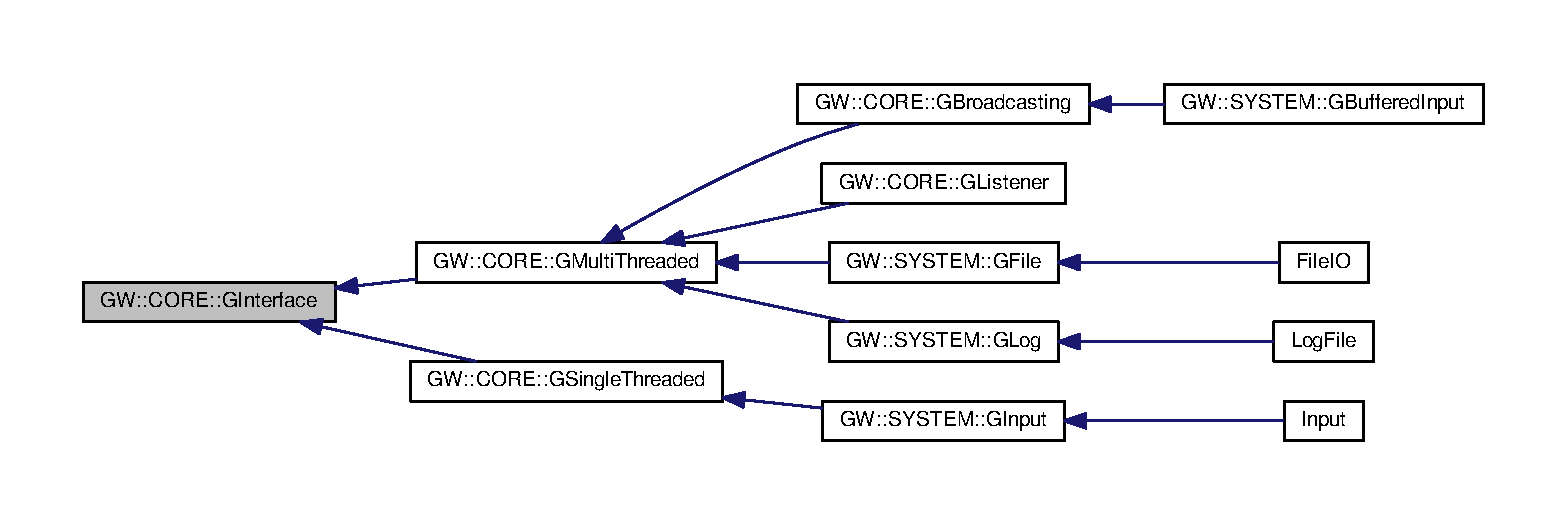
\includegraphics[width=350pt]{classGW_1_1CORE_1_1GInterface__inherit__graph}
\end{center}
\end{figure}
\subsection*{Public Member Functions}
\begin{DoxyCompactItemize}
\item 
virtual \hyperlink{namespaceGW_a67a839e3df7ea8a5c5686613a7a3de21}{G\+Return} \hyperlink{classGW_1_1CORE_1_1GInterface_aacf5834174a7024f8a3c361122ee9e76}{Get\+Count} (unsigned int \&\+\_\+out\+Count)=0
\begin{DoxyCompactList}\small\item\em Return the total number of active references to this object. \end{DoxyCompactList}\item 
virtual \hyperlink{namespaceGW_a67a839e3df7ea8a5c5686613a7a3de21}{G\+Return} \hyperlink{classGW_1_1CORE_1_1GInterface_a2d710f20bb78e544e8309b5b75c21260}{Increment\+Count} ()=0
\begin{DoxyCompactList}\small\item\em Increase the total number of active references to this object. \end{DoxyCompactList}\item 
virtual \hyperlink{namespaceGW_a67a839e3df7ea8a5c5686613a7a3de21}{G\+Return} \hyperlink{classGW_1_1CORE_1_1GInterface_a19a368c77ad0aa7f49b5a4f772f173ba}{Decrement\+Count} ()=0
\begin{DoxyCompactList}\small\item\em Decrease the total number of active references to this object. \end{DoxyCompactList}\item 
virtual \hyperlink{namespaceGW_a67a839e3df7ea8a5c5686613a7a3de21}{G\+Return} \hyperlink{classGW_1_1CORE_1_1GInterface_ad6c8324970172784964f484686d4fdad}{Request\+Interface} (const \hyperlink{structGW_1_1GUUIID}{G\+U\+U\+I\+ID} \&\+\_\+interface\+ID, void $\ast$$\ast$\+\_\+output\+Interface)=0
\begin{DoxyCompactList}\small\item\em Requests an interface that may or may not be supported by this object. \end{DoxyCompactList}\end{DoxyCompactItemize}


\subsection{Detailed Description}
Base interface all Gateware interfaces must support at a minimum. 

Core features include\+: Interface Upgrades, Reference Counting, Event Broadcasting. 

\subsection{Member Function Documentation}
\index{G\+W\+::\+C\+O\+R\+E\+::\+G\+Interface@{G\+W\+::\+C\+O\+R\+E\+::\+G\+Interface}!Decrement\+Count@{Decrement\+Count}}
\index{Decrement\+Count@{Decrement\+Count}!G\+W\+::\+C\+O\+R\+E\+::\+G\+Interface@{G\+W\+::\+C\+O\+R\+E\+::\+G\+Interface}}
\subsubsection[{\texorpdfstring{Decrement\+Count()=0}{DecrementCount()=0}}]{\setlength{\rightskip}{0pt plus 5cm}virtual {\bf G\+Return} G\+W\+::\+C\+O\+R\+E\+::\+G\+Interface\+::\+Decrement\+Count (
\begin{DoxyParamCaption}
{}
\end{DoxyParamCaption}
)\hspace{0.3cm}{\ttfamily [pure virtual]}}\hypertarget{classGW_1_1CORE_1_1GInterface_a19a368c77ad0aa7f49b5a4f772f173ba}{}\label{classGW_1_1CORE_1_1GInterface_a19a368c77ad0aa7f49b5a4f772f173ba}


Decrease the total number of active references to this object. 

Once the internal count reaches zero this object will be deallocated and your pointer will become invalid.


\begin{DoxyRetVals}{Return values}
{\em S\+U\+C\+C\+E\+SS} & Successfully decremented the internal reference count. \\
\hline
{\em F\+A\+I\+L\+U\+RE} & Decrementing of internal reference count would underflow the value. \\
\hline
\end{DoxyRetVals}


Implemented in \hyperlink{classFileIO_ab7e4806ca819c3fcdeeb40a2af5f0298}{File\+IO}, \hyperlink{classLogFile_a555ef35fcdce23ebad05f7dcabaf0757}{Log\+File}, and \hyperlink{classInput_a5c44b3dc2be21c1bad5f32a43a7b7a55}{Input}.

\index{G\+W\+::\+C\+O\+R\+E\+::\+G\+Interface@{G\+W\+::\+C\+O\+R\+E\+::\+G\+Interface}!Get\+Count@{Get\+Count}}
\index{Get\+Count@{Get\+Count}!G\+W\+::\+C\+O\+R\+E\+::\+G\+Interface@{G\+W\+::\+C\+O\+R\+E\+::\+G\+Interface}}
\subsubsection[{\texorpdfstring{Get\+Count(unsigned int \&\+\_\+out\+Count)=0}{GetCount(unsigned int &_outCount)=0}}]{\setlength{\rightskip}{0pt plus 5cm}virtual {\bf G\+Return} G\+W\+::\+C\+O\+R\+E\+::\+G\+Interface\+::\+Get\+Count (
\begin{DoxyParamCaption}
\item[{unsigned int \&}]{\+\_\+out\+Count}
\end{DoxyParamCaption}
)\hspace{0.3cm}{\ttfamily [pure virtual]}}\hypertarget{classGW_1_1CORE_1_1GInterface_aacf5834174a7024f8a3c361122ee9e76}{}\label{classGW_1_1CORE_1_1GInterface_aacf5834174a7024f8a3c361122ee9e76}


Return the total number of active references to this object. 


\begin{DoxyParams}[1]{Parameters}
\mbox{\tt out}  & {\em \+\_\+out\+Count} & The total number of active references of this object.\\
\hline
\end{DoxyParams}

\begin{DoxyRetVals}{Return values}
{\em S\+U\+C\+C\+E\+SS} & Successfully ran. \\
\hline
{\em F\+A\+I\+L\+U\+RE} & Either class does not exist or the internal reference count is corrupt. \\
\hline
\end{DoxyRetVals}


Implemented in \hyperlink{classFileIO_a20566e320ec4cc0d5615bc3bc1fa3013}{File\+IO}, \hyperlink{classLogFile_ab2abbdb01e2b904f112e5e7b20c59a81}{Log\+File}, and \hyperlink{classInput_a2fd6659ae76357836c4c9b3e7070ffb0}{Input}.

\index{G\+W\+::\+C\+O\+R\+E\+::\+G\+Interface@{G\+W\+::\+C\+O\+R\+E\+::\+G\+Interface}!Increment\+Count@{Increment\+Count}}
\index{Increment\+Count@{Increment\+Count}!G\+W\+::\+C\+O\+R\+E\+::\+G\+Interface@{G\+W\+::\+C\+O\+R\+E\+::\+G\+Interface}}
\subsubsection[{\texorpdfstring{Increment\+Count()=0}{IncrementCount()=0}}]{\setlength{\rightskip}{0pt plus 5cm}virtual {\bf G\+Return} G\+W\+::\+C\+O\+R\+E\+::\+G\+Interface\+::\+Increment\+Count (
\begin{DoxyParamCaption}
{}
\end{DoxyParamCaption}
)\hspace{0.3cm}{\ttfamily [pure virtual]}}\hypertarget{classGW_1_1CORE_1_1GInterface_a2d710f20bb78e544e8309b5b75c21260}{}\label{classGW_1_1CORE_1_1GInterface_a2d710f20bb78e544e8309b5b75c21260}


Increase the total number of active references to this object. 

End users should only call this operation if they are familiar with reference counting behavior.


\begin{DoxyRetVals}{Return values}
{\em S\+U\+C\+C\+E\+SS} & Successfully incremented the internal reference count. \\
\hline
{\em F\+A\+I\+L\+U\+RE} & Incrementation of internal reference count would overflow the value. \\
\hline
\end{DoxyRetVals}


Implemented in \hyperlink{classFileIO_a9f2c9a4d13577e14a2c94b0e9617d80b}{File\+IO}, \hyperlink{classLogFile_aff5871b4f2434b6ca722b89581416da0}{Log\+File}, and \hyperlink{classInput_a3c2103023cbb1fa583f910539bb6cce3}{Input}.

\index{G\+W\+::\+C\+O\+R\+E\+::\+G\+Interface@{G\+W\+::\+C\+O\+R\+E\+::\+G\+Interface}!Request\+Interface@{Request\+Interface}}
\index{Request\+Interface@{Request\+Interface}!G\+W\+::\+C\+O\+R\+E\+::\+G\+Interface@{G\+W\+::\+C\+O\+R\+E\+::\+G\+Interface}}
\subsubsection[{\texorpdfstring{Request\+Interface(const G\+U\+U\+I\+I\+D \&\+\_\+interface\+I\+D, void $\ast$$\ast$\+\_\+output\+Interface)=0}{RequestInterface(const GUUIID &_interfaceID, void **_outputInterface)=0}}]{\setlength{\rightskip}{0pt plus 5cm}virtual {\bf G\+Return} G\+W\+::\+C\+O\+R\+E\+::\+G\+Interface\+::\+Request\+Interface (
\begin{DoxyParamCaption}
\item[{const {\bf G\+U\+U\+I\+ID} \&}]{\+\_\+interface\+ID, }
\item[{void $\ast$$\ast$}]{\+\_\+output\+Interface}
\end{DoxyParamCaption}
)\hspace{0.3cm}{\ttfamily [pure virtual]}}\hypertarget{classGW_1_1CORE_1_1GInterface_ad6c8324970172784964f484686d4fdad}{}\label{classGW_1_1CORE_1_1GInterface_ad6c8324970172784964f484686d4fdad}


Requests an interface that may or may not be supported by this object. 

Can be used by the end-\/user to query for a new interface using the unique ID of the interface they want and implement an interface update.


\begin{DoxyParams}[1]{Parameters}
\mbox{\tt in}  & {\em \+\_\+interface\+ID} & The \hyperlink{structGW_1_1GUUIID}{G\+U\+U\+I\+ID} of the interface you are requesting. \\
\hline
\mbox{\tt out}  & {\em \+\_\+output\+Interface} & Where the interface will be stored if function is successful.\\
\hline
\end{DoxyParams}

\begin{DoxyRetVals}{Return values}
{\em S\+U\+C\+C\+E\+SS} & The interface is supported and function succeded. \\
\hline
{\em I\+N\+T\+E\+R\+F\+A\+C\+E\+\_\+\+U\+N\+S\+U\+P\+P\+O\+R\+T\+ED} & The requested interface is not supported. \\
\hline
\end{DoxyRetVals}


Implemented in \hyperlink{classFileIO_a3fb39527fac479474c6ef5045dbc1551}{File\+IO}, \hyperlink{classLogFile_a8b8e63b9c62846b1b9e0cf8b79429ba5}{Log\+File}, and \hyperlink{classInput_a29f3c56e9fec9f9073c1e18f120a69cd}{Input}.



The documentation for this class was generated from the following file\+:\begin{DoxyCompactItemize}
\item 
Interface/\+G\+\_\+\+Core/G\+Interface.\+h\end{DoxyCompactItemize}

\hypertarget{interfaceGIResponder}{}\section{G\+I\+Responder Class Reference}
\label{interfaceGIResponder}\index{G\+I\+Responder@{G\+I\+Responder}}


Inheritance diagram for G\+I\+Responder\+:
\nopagebreak
\begin{figure}[H]
\begin{center}
\leavevmode
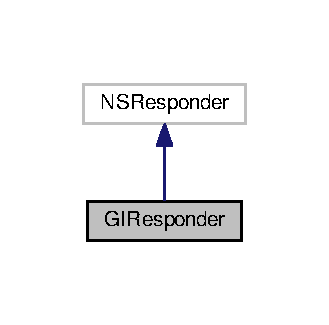
\includegraphics[width=158pt]{interfaceGIResponder__inherit__graph}
\end{center}
\end{figure}


Collaboration diagram for G\+I\+Responder\+:
\nopagebreak
\begin{figure}[H]
\begin{center}
\leavevmode
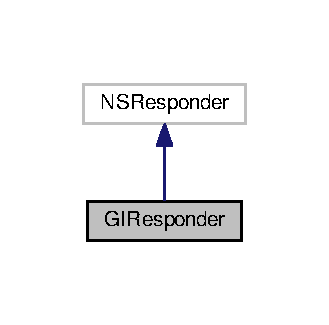
\includegraphics[width=158pt]{interfaceGIResponder__coll__graph}
\end{center}
\end{figure}
\subsection*{Instance Methods}
\begin{DoxyCompactItemize}
\item 
(bool) -\/ {\bfseries accept\+First\+Responder}\hypertarget{interfaceGIResponder_a69336360b238bdbdc953846ffd8ec680}{}\label{interfaceGIResponder_a69336360b238bdbdc953846ffd8ec680}

\item 
(bool) -\/ {\bfseries accepts\+First\+Mouse\+:}\hypertarget{interfaceGIResponder_a7c7a4084b23e4fbbdf87d1aef1aef090}{}\label{interfaceGIResponder_a7c7a4084b23e4fbbdf87d1aef1aef090}

\item 
(void) -\/ {\bfseries key\+Down\+:}\hypertarget{interfaceGIResponder_a4cabb99dc9bb76c07c5528881f7ca9ef}{}\label{interfaceGIResponder_a4cabb99dc9bb76c07c5528881f7ca9ef}

\item 
(void) -\/ {\bfseries key\+Up\+:}\hypertarget{interfaceGIResponder_a2a3be3ad8c5f0bc96b0f4d0006f69581}{}\label{interfaceGIResponder_a2a3be3ad8c5f0bc96b0f4d0006f69581}

\item 
(void) -\/ {\bfseries mouse\+Down\+:}\hypertarget{interfaceGIResponder_a177aff5b20126cb7968706cbb81195c2}{}\label{interfaceGIResponder_a177aff5b20126cb7968706cbb81195c2}

\item 
(void) -\/ {\bfseries mouse\+Up\+:}\hypertarget{interfaceGIResponder_a95d3d4ce7947363452eab0e158e9ebef}{}\label{interfaceGIResponder_a95d3d4ce7947363452eab0e158e9ebef}

\item 
(void) -\/ {\bfseries rightmouse\+Down\+:}\hypertarget{interfaceGIResponder_a51426c29065c07f9e2afbbc8181d6b74}{}\label{interfaceGIResponder_a51426c29065c07f9e2afbbc8181d6b74}

\item 
(void) -\/ {\bfseries rightmouse\+Up\+:}\hypertarget{interfaceGIResponder_abe9b61c47fa25f70ab6a82417979b3b7}{}\label{interfaceGIResponder_abe9b61c47fa25f70ab6a82417979b3b7}

\item 
(void) -\/ {\bfseries othermouse\+Down\+:}\hypertarget{interfaceGIResponder_a4796bfaa60025ff0631b525fd52b2182}{}\label{interfaceGIResponder_a4796bfaa60025ff0631b525fd52b2182}

\item 
(void) -\/ {\bfseries othermouse\+Up\+:}\hypertarget{interfaceGIResponder_a88e82a046893b9aab9f0776173ba6ee8}{}\label{interfaceGIResponder_a88e82a046893b9aab9f0776173ba6ee8}

\item 
(void) -\/ {\bfseries mouse\+Moved\+:}\hypertarget{interfaceGIResponder_a699c6208ac80a3c6d3c4abb222a03a10}{}\label{interfaceGIResponder_a699c6208ac80a3c6d3c4abb222a03a10}

\item 
(void) -\/ {\bfseries Get\+Key\+Mask\+:}\hypertarget{interfaceGIResponder_a060835ad8e859fca137acaee50593a47}{}\label{interfaceGIResponder_a060835ad8e859fca137acaee50593a47}

\end{DoxyCompactItemize}
\subsection*{Protected Attributes}
\begin{DoxyCompactItemize}
\item 
N\+S\+U\+Integer {\bfseries flags}\hypertarget{interfaceGIResponder_acbb29dd4a78a53d141da79b551fc82a5}{}\label{interfaceGIResponder_acbb29dd4a78a53d141da79b551fc82a5}

\end{DoxyCompactItemize}


The documentation for this class was generated from the following file\+:\begin{DoxyCompactItemize}
\item 
Source/\+G\+\_\+\+System/G\+Input.\+mm\end{DoxyCompactItemize}

\hypertarget{classGW_1_1CORE_1_1GListener}{}\section{GW\+::C\+O\+RE\+::G\+Listener Class Reference}
\label{classGW_1_1CORE_1_1GListener}\index{GW::CORE::GListener@{GW::CORE::GListener}}


A \mbox{\hyperlink{classGW_1_1CORE_1_1GListener}{G\+Listener}} Interface may be registered with a G\+Broadcaster interface to receive event notifications.  




{\ttfamily \#include $<$G\+Listener.\+h$>$}



Inheritance diagram for GW\+::C\+O\+RE\+::G\+Listener\+:
% FIG 0


Collaboration diagram for GW\+::C\+O\+RE\+::G\+Listener\+:
% FIG 1
\subsection*{Public Member Functions}
\begin{DoxyCompactItemize}
\item 
virtual \mbox{\hyperlink{namespaceGW_a67a839e3df7ea8a5c5686613a7a3de21}{G\+Return}} \mbox{\hyperlink{classGW_1_1CORE_1_1GListener_a5c1d1fac213b7a1cc15d384aa0c33105}{On\+Event}} (const \mbox{\hyperlink{structGW_1_1GUUIID}{G\+U\+U\+I\+ID}} \&\+\_\+sender\+Interface, unsigned int \+\_\+event\+ID, void $\ast$\+\_\+event\+Data, unsigned int \+\_\+data\+Size)=0
\begin{DoxyCompactList}\small\item\em This operation is called whenever a G\+Broadcaster a listener is registered to generates an event. \end{DoxyCompactList}\end{DoxyCompactItemize}


\subsection{Detailed Description}
A \mbox{\hyperlink{classGW_1_1CORE_1_1GListener}{G\+Listener}} Interface may be registered with a G\+Broadcaster interface to receive event notifications. 

\mbox{\hyperlink{classGW_1_1CORE_1_1GListener}{G\+Listener}} is directly inherited from \mbox{\hyperlink{classGW_1_1CORE_1_1GMultiThreaded}{G\+Multi\+Threaded}}, therefore its implementation must be thread safe. 

\subsection{Member Function Documentation}
\mbox{\Hypertarget{classGW_1_1CORE_1_1GListener_a5c1d1fac213b7a1cc15d384aa0c33105}\label{classGW_1_1CORE_1_1GListener_a5c1d1fac213b7a1cc15d384aa0c33105}} 
\index{GW::CORE::GListener@{GW::CORE::GListener}!OnEvent@{OnEvent}}
\index{OnEvent@{OnEvent}!GW::CORE::GListener@{GW::CORE::GListener}}
\subsubsection{\texorpdfstring{OnEvent()}{OnEvent()}}
{\footnotesize\ttfamily virtual \mbox{\hyperlink{namespaceGW_a67a839e3df7ea8a5c5686613a7a3de21}{G\+Return}} G\+W\+::\+C\+O\+R\+E\+::\+G\+Listener\+::\+On\+Event (\begin{DoxyParamCaption}\item[{const \mbox{\hyperlink{structGW_1_1GUUIID}{G\+U\+U\+I\+ID}} \&}]{\+\_\+sender\+Interface,  }\item[{unsigned int}]{\+\_\+event\+ID,  }\item[{void $\ast$}]{\+\_\+event\+Data,  }\item[{unsigned int}]{\+\_\+data\+Size }\end{DoxyParamCaption})\hspace{0.3cm}{\ttfamily [pure virtual]}}



This operation is called whenever a G\+Broadcaster a listener is registered to generates an event. 


\begin{DoxyParams}[1]{Parameters}
\mbox{\texttt{ in}}  & {\em \+\_\+sender\+Interface} & The interface of the sender object. \\
\hline
\mbox{\texttt{ in}}  & {\em \+\_\+event\+ID} & The ID of the event sent. \\
\hline
\mbox{\texttt{ in}}  & {\em \+\_\+event\+Data} & The data of the event. \\
\hline
\mbox{\texttt{ in}}  & {\em \+\_\+data\+Size} & The size of \+\_\+event\+Data in bytes. \\
\hline
\end{DoxyParams}


The documentation for this class was generated from the following file\+:\begin{DoxyCompactItemize}
\item 
Interface/\+G\+\_\+\+Core/G\+Listener.\+h\end{DoxyCompactItemize}

\hypertarget{classGW_1_1SYSTEM_1_1GLog}{}\section{GW\+:\+:S\+Y\+S\+T\+EM\+:\+:G\+Log Class Reference}
\label{classGW_1_1SYSTEM_1_1GLog}\index{G\+W\+::\+S\+Y\+S\+T\+E\+M\+::\+G\+Log@{G\+W\+::\+S\+Y\+S\+T\+E\+M\+::\+G\+Log}}


Cross platform threadsafe logger.  




{\ttfamily \#include $<$G\+Log.\+h$>$}



Inheritance diagram for GW\+:\+:S\+Y\+S\+T\+EM\+:\+:G\+Log\+:
\nopagebreak
\begin{figure}[H]
\begin{center}
\leavevmode
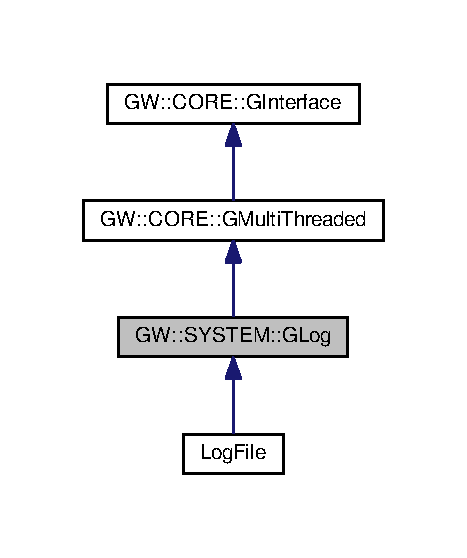
\includegraphics[width=224pt]{classGW_1_1SYSTEM_1_1GLog__inherit__graph}
\end{center}
\end{figure}


Collaboration diagram for GW\+:\+:S\+Y\+S\+T\+EM\+:\+:G\+Log\+:
\nopagebreak
\begin{figure}[H]
\begin{center}
\leavevmode
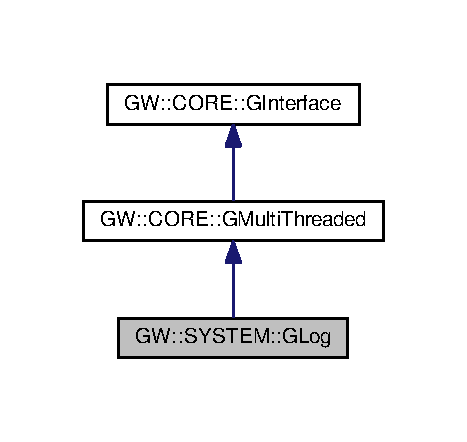
\includegraphics[width=224pt]{classGW_1_1SYSTEM_1_1GLog__coll__graph}
\end{center}
\end{figure}
\subsection*{Public Member Functions}
\begin{DoxyCompactItemize}
\item 
virtual \hyperlink{namespaceGW_a67a839e3df7ea8a5c5686613a7a3de21}{G\+Return} \hyperlink{classGW_1_1SYSTEM_1_1GLog_a9e21e702d012065fe799b4c49f7ac670}{Log} (const char $\ast$const \+\_\+log)=0
\begin{DoxyCompactList}\small\item\em Logs a null terminated string. \end{DoxyCompactList}\item 
virtual \hyperlink{namespaceGW_a67a839e3df7ea8a5c5686613a7a3de21}{G\+Return} \hyperlink{classGW_1_1SYSTEM_1_1GLog_a5d10397fa6aeeebaf8430df6029ec3c5}{Log\+Catergorized} (const char $\ast$const \+\_\+category, const char $\ast$const \+\_\+log)=0
\begin{DoxyCompactList}\small\item\em Logs a null terminated string with a category. \end{DoxyCompactList}\item 
virtual void \hyperlink{classGW_1_1SYSTEM_1_1GLog_a4323c96541a34fb0344828a1c20ec254}{Enable\+Verbose\+Logging} (bool \+\_\+value)=0
\begin{DoxyCompactList}\small\item\em Turns verbose logging on or off. \end{DoxyCompactList}\item 
virtual void \hyperlink{classGW_1_1SYSTEM_1_1GLog_abceb9fdf502b11f2fe72de5edd8f187d}{Enable\+Console\+Logging} (bool \+\_\+value)=0
\begin{DoxyCompactList}\small\item\em Turns console logging on or off. \end{DoxyCompactList}\item 
virtual \hyperlink{namespaceGW_a67a839e3df7ea8a5c5686613a7a3de21}{G\+Return} \hyperlink{classGW_1_1SYSTEM_1_1GLog_a07147c15ecb17caa1c83974b3c54f7d4}{Flush} ()=0
\begin{DoxyCompactList}\small\item\em Forces a log dump to file. \end{DoxyCompactList}\end{DoxyCompactItemize}


\subsection{Detailed Description}
Cross platform threadsafe logger. 

\hyperlink{classGW_1_1SYSTEM_1_1GLog}{G\+Log} inherits directly from G\+Multi\+Threaded, therefore its implementation must be thread safe. 

\subsection{Member Function Documentation}
\index{G\+W\+::\+S\+Y\+S\+T\+E\+M\+::\+G\+Log@{G\+W\+::\+S\+Y\+S\+T\+E\+M\+::\+G\+Log}!Enable\+Console\+Logging@{Enable\+Console\+Logging}}
\index{Enable\+Console\+Logging@{Enable\+Console\+Logging}!G\+W\+::\+S\+Y\+S\+T\+E\+M\+::\+G\+Log@{G\+W\+::\+S\+Y\+S\+T\+E\+M\+::\+G\+Log}}
\subsubsection[{\texorpdfstring{Enable\+Console\+Logging(bool \+\_\+value)=0}{EnableConsoleLogging(bool _value)=0}}]{\setlength{\rightskip}{0pt plus 5cm}virtual void G\+W\+::\+S\+Y\+S\+T\+E\+M\+::\+G\+Log\+::\+Enable\+Console\+Logging (
\begin{DoxyParamCaption}
\item[{bool}]{\+\_\+value}
\end{DoxyParamCaption}
)\hspace{0.3cm}{\ttfamily [pure virtual]}}\hypertarget{classGW_1_1SYSTEM_1_1GLog_abceb9fdf502b11f2fe72de5edd8f187d}{}\label{classGW_1_1SYSTEM_1_1GLog_abceb9fdf502b11f2fe72de5edd8f187d}


Turns console logging on or off. 

Use this function to ensure or prevent the additional console logging.


\begin{DoxyParams}[1]{Parameters}
\mbox{\tt in}  & {\em \+\_\+value} & true to turn on or false to turn off. \\
\hline
\end{DoxyParams}


Implemented in \hyperlink{classLogFile_a903b31947e1c100309dcc5b20548262c}{Log\+File}.

\index{G\+W\+::\+S\+Y\+S\+T\+E\+M\+::\+G\+Log@{G\+W\+::\+S\+Y\+S\+T\+E\+M\+::\+G\+Log}!Enable\+Verbose\+Logging@{Enable\+Verbose\+Logging}}
\index{Enable\+Verbose\+Logging@{Enable\+Verbose\+Logging}!G\+W\+::\+S\+Y\+S\+T\+E\+M\+::\+G\+Log@{G\+W\+::\+S\+Y\+S\+T\+E\+M\+::\+G\+Log}}
\subsubsection[{\texorpdfstring{Enable\+Verbose\+Logging(bool \+\_\+value)=0}{EnableVerboseLogging(bool _value)=0}}]{\setlength{\rightskip}{0pt plus 5cm}virtual void G\+W\+::\+S\+Y\+S\+T\+E\+M\+::\+G\+Log\+::\+Enable\+Verbose\+Logging (
\begin{DoxyParamCaption}
\item[{bool}]{\+\_\+value}
\end{DoxyParamCaption}
)\hspace{0.3cm}{\ttfamily [pure virtual]}}\hypertarget{classGW_1_1SYSTEM_1_1GLog_a4323c96541a34fb0344828a1c20ec254}{}\label{classGW_1_1SYSTEM_1_1GLog_a4323c96541a34fb0344828a1c20ec254}


Turns verbose logging on or off. 

Use this function to ensure or prevent the addition of date, time, and thread\+ID to your log messages.


\begin{DoxyParams}[1]{Parameters}
\mbox{\tt in}  & {\em \+\_\+value} & true to turn on or false to turn off. \\
\hline
\end{DoxyParams}


Implemented in \hyperlink{classLogFile_a250bcfaccded12f7da9a06b6f6336fa5}{Log\+File}.

\index{G\+W\+::\+S\+Y\+S\+T\+E\+M\+::\+G\+Log@{G\+W\+::\+S\+Y\+S\+T\+E\+M\+::\+G\+Log}!Flush@{Flush}}
\index{Flush@{Flush}!G\+W\+::\+S\+Y\+S\+T\+E\+M\+::\+G\+Log@{G\+W\+::\+S\+Y\+S\+T\+E\+M\+::\+G\+Log}}
\subsubsection[{\texorpdfstring{Flush()=0}{Flush()=0}}]{\setlength{\rightskip}{0pt plus 5cm}virtual {\bf G\+Return} G\+W\+::\+S\+Y\+S\+T\+E\+M\+::\+G\+Log\+::\+Flush (
\begin{DoxyParamCaption}
{}
\end{DoxyParamCaption}
)\hspace{0.3cm}{\ttfamily [pure virtual]}}\hypertarget{classGW_1_1SYSTEM_1_1GLog_a07147c15ecb17caa1c83974b3c54f7d4}{}\label{classGW_1_1SYSTEM_1_1GLog_a07147c15ecb17caa1c83974b3c54f7d4}


Forces a log dump to file. 

This will force a log dump to the file and clear the log queue.


\begin{DoxyRetVals}{Return values}
{\em S\+U\+C\+C\+E\+SS} & Successfully dumped the logs. \\
\hline
{\em F\+A\+I\+L\+U\+RE} & Most likely a file corruption or a file is not open. \\
\hline
\end{DoxyRetVals}


Implemented in \hyperlink{classLogFile_a47ffb41f72625b1c7865ac2cd58dea18}{Log\+File}.

\index{G\+W\+::\+S\+Y\+S\+T\+E\+M\+::\+G\+Log@{G\+W\+::\+S\+Y\+S\+T\+E\+M\+::\+G\+Log}!Log@{Log}}
\index{Log@{Log}!G\+W\+::\+S\+Y\+S\+T\+E\+M\+::\+G\+Log@{G\+W\+::\+S\+Y\+S\+T\+E\+M\+::\+G\+Log}}
\subsubsection[{\texorpdfstring{Log(const char $\ast$const \+\_\+log)=0}{Log(const char *const _log)=0}}]{\setlength{\rightskip}{0pt plus 5cm}virtual {\bf G\+Return} G\+W\+::\+S\+Y\+S\+T\+E\+M\+::\+G\+Log\+::\+Log (
\begin{DoxyParamCaption}
\item[{const char $\ast$const}]{\+\_\+log}
\end{DoxyParamCaption}
)\hspace{0.3cm}{\ttfamily [pure virtual]}}\hypertarget{classGW_1_1SYSTEM_1_1GLog_a9e21e702d012065fe799b4c49f7ac670}{}\label{classGW_1_1SYSTEM_1_1GLog_a9e21e702d012065fe799b4c49f7ac670}


Logs a null terminated string. 

Date, Time, and thread ID will be appended to the front of the message unless specified otherwise (See Enable\+Verbose\+Logging). A new line character will be appended to the end of the string so your log messages do not require a new line. The string is logged to the internal \hyperlink{classGW_1_1SYSTEM_1_1GFile}{G\+File} object.


\begin{DoxyParams}[1]{Parameters}
\mbox{\tt in}  & {\em \+\_\+log} & The message to log out.\\
\hline
\end{DoxyParams}

\begin{DoxyRetVals}{Return values}
{\em S\+U\+C\+C\+E\+SS} & Successfully queued the message to the log. \\
\hline
{\em F\+A\+I\+L\+U\+RE} & The queue has reached maximum size (call flush). \\
\hline
{\em I\+N\+V\+A\+L\+I\+D\+\_\+\+A\+R\+G\+U\+M\+E\+NT} & A nullptr was passed in. \\
\hline
\end{DoxyRetVals}


Implemented in \hyperlink{classLogFile_a6848c12fad15f2c835e5215234f75c5a}{Log\+File}.

\index{G\+W\+::\+S\+Y\+S\+T\+E\+M\+::\+G\+Log@{G\+W\+::\+S\+Y\+S\+T\+E\+M\+::\+G\+Log}!Log\+Catergorized@{Log\+Catergorized}}
\index{Log\+Catergorized@{Log\+Catergorized}!G\+W\+::\+S\+Y\+S\+T\+E\+M\+::\+G\+Log@{G\+W\+::\+S\+Y\+S\+T\+E\+M\+::\+G\+Log}}
\subsubsection[{\texorpdfstring{Log\+Catergorized(const char $\ast$const \+\_\+category, const char $\ast$const \+\_\+log)=0}{LogCatergorized(const char *const _category, const char *const _log)=0}}]{\setlength{\rightskip}{0pt plus 5cm}virtual {\bf G\+Return} G\+W\+::\+S\+Y\+S\+T\+E\+M\+::\+G\+Log\+::\+Log\+Catergorized (
\begin{DoxyParamCaption}
\item[{const char $\ast$const}]{\+\_\+category, }
\item[{const char $\ast$const}]{\+\_\+log}
\end{DoxyParamCaption}
)\hspace{0.3cm}{\ttfamily [pure virtual]}}\hypertarget{classGW_1_1SYSTEM_1_1GLog_a5d10397fa6aeeebaf8430df6029ec3c5}{}\label{classGW_1_1SYSTEM_1_1GLog_a5d10397fa6aeeebaf8430df6029ec3c5}


Logs a null terminated string with a category. 

Date, Time, and thread ID will be appended to the front of the message unless specified otherwise (See Enable\+Verbose\+Logging). A new line character will be appended to the end of the string so your log messages do not require a new line. The string is logged to the internal \hyperlink{classGW_1_1SYSTEM_1_1GFile}{G\+File} object.


\begin{DoxyParams}[1]{Parameters}
\mbox{\tt in}  & {\em \+\_\+category} & The category the log belongs in. ie. E\+R\+R\+OR, W\+A\+R\+N\+I\+NG, I\+N\+FO, etc. \\
\hline
\mbox{\tt in}  & {\em \+\_\+log} & The message to log out.\\
\hline
\end{DoxyParams}

\begin{DoxyRetVals}{Return values}
{\em S\+U\+C\+C\+E\+SS} & Successfully queued the message to the log. \\
\hline
{\em F\+A\+I\+L\+U\+RE} & The queue has reached maximum size (call flush). \\
\hline
{\em I\+N\+V\+A\+L\+I\+D\+\_\+\+A\+R\+G\+U\+M\+E\+NT} & Either \+\_\+category or \+\_\+log are nullptr. \\
\hline
\end{DoxyRetVals}


Implemented in \hyperlink{classLogFile_a5e5f24ccd4c6f925dd8bc1ced512b530}{Log\+File}.



The documentation for this class was generated from the following file\+:\begin{DoxyCompactItemize}
\item 
Interface/\+G\+\_\+\+System/G\+Log.\+h\end{DoxyCompactItemize}

\hypertarget{classGW_1_1CORE_1_1GMultiThreaded}{}\section{GW\+::C\+O\+RE\+::G\+Multi\+Threaded Class Reference}
\label{classGW_1_1CORE_1_1GMultiThreaded}\index{GW::CORE::GMultiThreaded@{GW::CORE::GMultiThreaded}}


This interface is only used to label and query interfaces which promise to 100\% internally support thread safety.  




{\ttfamily \#include $<$G\+Multi\+Threaded.\+h$>$}



Inheritance diagram for GW\+::C\+O\+RE\+::G\+Multi\+Threaded\+:
% FIG 0


Collaboration diagram for GW\+::C\+O\+RE\+::G\+Multi\+Threaded\+:
% FIG 1
\subsection*{Additional Inherited Members}


\subsection{Detailed Description}
This interface is only used to label and query interfaces which promise to 100\% internally support thread safety. 

The documentation for this class was generated from the following file\+:\begin{DoxyCompactItemize}
\item 
Interface/\+G\+\_\+\+Core/G\+Multi\+Threaded.\+h\end{DoxyCompactItemize}

\hypertarget{interfaceGResponder}{}\section{G\+Responder Class Reference}
\label{interfaceGResponder}\index{G\+Responder@{G\+Responder}}


Inheritance diagram for G\+Responder\+:
\nopagebreak
\begin{figure}[H]
\begin{center}
\leavevmode
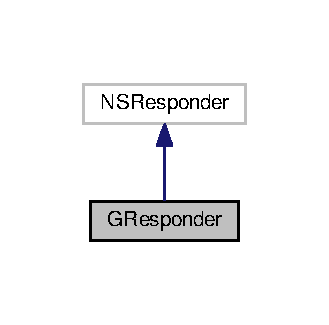
\includegraphics[width=158pt]{interfaceGResponder__inherit__graph}
\end{center}
\end{figure}


Collaboration diagram for G\+Responder\+:
\nopagebreak
\begin{figure}[H]
\begin{center}
\leavevmode
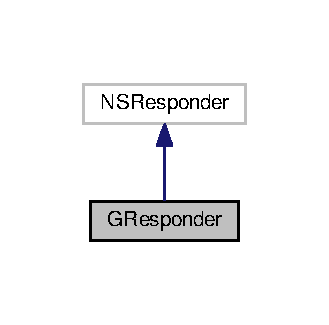
\includegraphics[width=158pt]{interfaceGResponder__coll__graph}
\end{center}
\end{figure}
\subsection*{Instance Methods}
\begin{DoxyCompactItemize}
\item 
(bool) -\/ {\bfseries accept\+First\+Responder}\hypertarget{interfaceGResponder_a38d089c6fa50dadb001917d4376136c5}{}\label{interfaceGResponder_a38d089c6fa50dadb001917d4376136c5}

\item 
(bool) -\/ {\bfseries accepts\+First\+Mouse\+:}\hypertarget{interfaceGResponder_a9358ee727560f1a9fa05b063051bf425}{}\label{interfaceGResponder_a9358ee727560f1a9fa05b063051bf425}

\item 
(void) -\/ {\bfseries key\+Down\+:}\hypertarget{interfaceGResponder_a546f385e994c7eb9fcf16a244c0ecef6}{}\label{interfaceGResponder_a546f385e994c7eb9fcf16a244c0ecef6}

\item 
(void) -\/ {\bfseries key\+Up\+:}\hypertarget{interfaceGResponder_a6474d631363b8835109a5d0934aa84bf}{}\label{interfaceGResponder_a6474d631363b8835109a5d0934aa84bf}

\item 
(void) -\/ {\bfseries mouse\+Down\+:}\hypertarget{interfaceGResponder_ae5fe08f8848c8ee139da21ebac0b2204}{}\label{interfaceGResponder_ae5fe08f8848c8ee139da21ebac0b2204}

\item 
(void) -\/ {\bfseries mouse\+Up\+:}\hypertarget{interfaceGResponder_aebc62bc4faf4cf99635a1481eca99004}{}\label{interfaceGResponder_aebc62bc4faf4cf99635a1481eca99004}

\item 
(void) -\/ {\bfseries rightmouse\+Down\+:}\hypertarget{interfaceGResponder_a25f874602d27e9e8c8601e3524bee880}{}\label{interfaceGResponder_a25f874602d27e9e8c8601e3524bee880}

\item 
(void) -\/ {\bfseries rightmouse\+Up\+:}\hypertarget{interfaceGResponder_a20a0b3baac9815710c7d62f1df1d9165}{}\label{interfaceGResponder_a20a0b3baac9815710c7d62f1df1d9165}

\item 
(void) -\/ {\bfseries othermouse\+Down\+:}\hypertarget{interfaceGResponder_a47a3c5d341c5d5066ab91b2e0746b438}{}\label{interfaceGResponder_a47a3c5d341c5d5066ab91b2e0746b438}

\item 
(void) -\/ {\bfseries othermouse\+Up\+:}\hypertarget{interfaceGResponder_a8e07cdcdc82a14526a6b0ebf1b1db458}{}\label{interfaceGResponder_a8e07cdcdc82a14526a6b0ebf1b1db458}

\item 
(void) -\/ {\bfseries scroll\+Wheel\+:}\hypertarget{interfaceGResponder_af419f86d1634b577f9749a3ad0bf2040}{}\label{interfaceGResponder_af419f86d1634b577f9749a3ad0bf2040}

\item 
(void) -\/ {\bfseries Get\+Key\+Mask\+:}\hypertarget{interfaceGResponder_ae59e6d264d257ca2c6068f6dd861ae8c}{}\label{interfaceGResponder_ae59e6d264d257ca2c6068f6dd861ae8c}

\end{DoxyCompactItemize}


The documentation for this class was generated from the following file\+:\begin{DoxyCompactItemize}
\item 
Source/\+G\+\_\+\+System/G\+Buffered\+Input.\+mm\end{DoxyCompactItemize}

\hypertarget{classGW_1_1CORE_1_1GSingleThreaded}{}\section{GW\+::C\+O\+RE\+::G\+Single\+Threaded Class Reference}
\label{classGW_1_1CORE_1_1GSingleThreaded}\index{GW::CORE::GSingleThreaded@{GW::CORE::GSingleThreaded}}


This interface is only used to label and query interfaces which are not designed internally to support thread safety.  




{\ttfamily \#include $<$G\+Single\+Threaded.\+h$>$}



Inheritance diagram for GW\+::C\+O\+RE\+::G\+Single\+Threaded\+:
% FIG 0


Collaboration diagram for GW\+::C\+O\+RE\+::G\+Single\+Threaded\+:
% FIG 1
\subsection*{Additional Inherited Members}


\subsection{Detailed Description}
This interface is only used to label and query interfaces which are not designed internally to support thread safety. 

The documentation for this class was generated from the following file\+:\begin{DoxyCompactItemize}
\item 
Interface/\+G\+\_\+\+Core/G\+Single\+Threaded.\+h\end{DoxyCompactItemize}

\hypertarget{structGW_1_1GUUIID}{}\section{GW\+:\+:G\+U\+U\+I\+ID Struct Reference}
\label{structGW_1_1GUUIID}\index{G\+W\+::\+G\+U\+U\+I\+ID@{G\+W\+::\+G\+U\+U\+I\+ID}}


Gateware Universally Unique Interface I\+Dentifier.  




{\ttfamily \#include $<$G\+Defines.\+h$>$}

\subsection*{Public Member Functions}
\begin{DoxyCompactItemize}
\item 
bool \hyperlink{structGW_1_1GUUIID_a84e8d2cc912c79229af8dd9a898e1ace}{operator==} (const \hyperlink{structGW_1_1GUUIID}{G\+U\+U\+I\+ID} \&\+\_\+cmp) const \hypertarget{structGW_1_1GUUIID_a84e8d2cc912c79229af8dd9a898e1ace}{}\label{structGW_1_1GUUIID_a84e8d2cc912c79229af8dd9a898e1ace}

\begin{DoxyCompactList}\small\item\em Comparison operator overload. \end{DoxyCompactList}\end{DoxyCompactItemize}
\subsection*{Public Attributes}
\begin{DoxyCompactItemize}
\item 
\begin{tabbing}
xx\=xx\=xx\=xx\=xx\=xx\=xx\=xx\=xx\=\kill
union \{\\
\>struct \{\\
\>\>unsigned int {\bfseries byte4}\\
\>\>unsigned short {\bfseries byte2a}\\
\>\>unsigned short {\bfseries byte2b}\\
\>\>unsigned char {\bfseries byte8} \mbox{[}8\mbox{]}\\
\>\} \hypertarget{unionGW_1_1GUUIID_1_1_0D0_a408b2437c2ea63a4cb75888db0ac62fb}{}\label{unionGW_1_1GUUIID_1_1_0D0_a408b2437c2ea63a4cb75888db0ac62fb}
\\
\>unsigned long long {\bfseries parts} \mbox{[}2\mbox{]}\\
\}; \hypertarget{structGW_1_1GUUIID_aa51f004bf72e52a4e15b7568b9a7ec50}{}\label{structGW_1_1GUUIID_aa51f004bf72e52a4e15b7568b9a7ec50}
\\

\end{tabbing}\end{DoxyCompactItemize}


\subsection{Detailed Description}
Gateware Universally Unique Interface I\+Dentifier. 

Each \hyperlink{structGW_1_1GUUIID}{G\+U\+U\+I\+ID} defines a unique 128bit number identifying a particular version of an interface. This allows interfaces to be upgraded down the line safely without breaking legacy code. 

The documentation for this struct was generated from the following file\+:\begin{DoxyCompactItemize}
\item 
Interface/\+G\+\_\+\+Core/G\+Defines.\+h\end{DoxyCompactItemize}

\hypertarget{interfaceGWAppDelegate}{}\section{G\+W\+App\+Delegate Class Reference}
\label{interfaceGWAppDelegate}\index{G\+W\+App\+Delegate@{G\+W\+App\+Delegate}}


Inheritance diagram for G\+W\+App\+Delegate\+:
\nopagebreak
\begin{figure}[H]
\begin{center}
\leavevmode
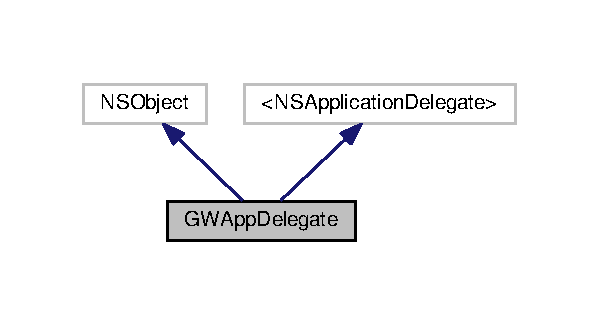
\includegraphics[width=288pt]{interfaceGWAppDelegate__inherit__graph}
\end{center}
\end{figure}


Collaboration diagram for G\+W\+App\+Delegate\+:
\nopagebreak
\begin{figure}[H]
\begin{center}
\leavevmode
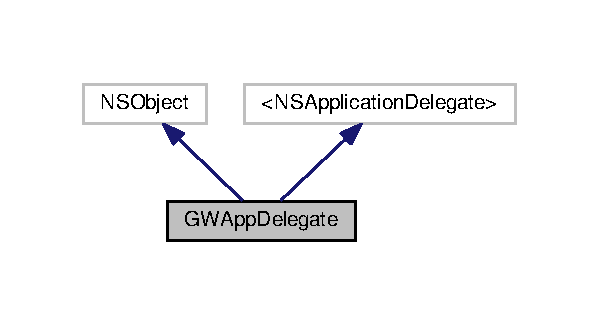
\includegraphics[width=288pt]{interfaceGWAppDelegate__coll__graph}
\end{center}
\end{figure}
\subsection*{Instance Methods}
\begin{DoxyCompactItemize}
\item 
(void) -\/ {\bfseries application\+Did\+Finish\+Launching\+:}\hypertarget{interfaceGWAppDelegate_a7d719bcad8b9e126701331457d9f9456}{}\label{interfaceGWAppDelegate_a7d719bcad8b9e126701331457d9f9456}

\end{DoxyCompactItemize}


The documentation for this class was generated from the following file\+:\begin{DoxyCompactItemize}
\item 
Source/\+G\+\_\+\+System/G\+Window.\+mm\end{DoxyCompactItemize}

\hypertarget{interfaceGWDelegate}{}\section{G\+W\+Delegate Class Reference}
\label{interfaceGWDelegate}\index{G\+W\+Delegate@{G\+W\+Delegate}}


Inheritance diagram for G\+W\+Delegate\+:
\nopagebreak
\begin{figure}[H]
\begin{center}
\leavevmode
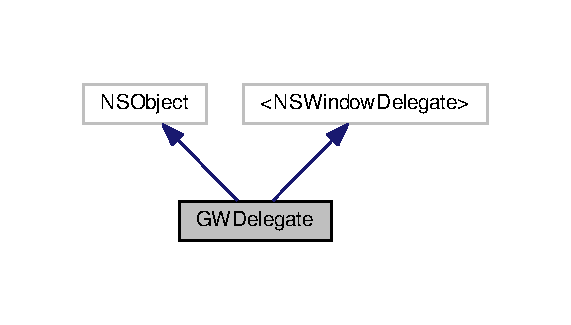
\includegraphics[width=274pt]{interfaceGWDelegate__inherit__graph}
\end{center}
\end{figure}


Collaboration diagram for G\+W\+Delegate\+:
\nopagebreak
\begin{figure}[H]
\begin{center}
\leavevmode
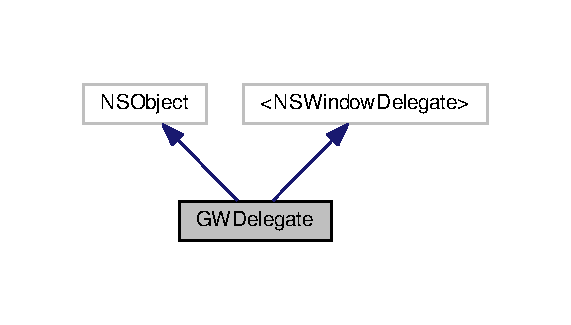
\includegraphics[width=274pt]{interfaceGWDelegate__coll__graph}
\end{center}
\end{figure}
\subsection*{Instance Methods}
\begin{DoxyCompactItemize}
\item 
(N\+S\+Size) -\/ {\bfseries window\+Will\+Resize\+:to\+Size\+:}\hypertarget{interfaceGWDelegate_abfdd429cc49d59b4df11246a60bf408f}{}\label{interfaceGWDelegate_abfdd429cc49d59b4df11246a60bf408f}

\item 
(void) -\/ {\bfseries window\+Did\+Resize\+:}\hypertarget{interfaceGWDelegate_a665568e3f51c44e4231ad609e4151a9b}{}\label{interfaceGWDelegate_a665568e3f51c44e4231ad609e4151a9b}

\item 
(void) -\/ {\bfseries window\+Did\+Move\+:}\hypertarget{interfaceGWDelegate_a84abecd6d6a492efb9db7fe3470286d6}{}\label{interfaceGWDelegate_a84abecd6d6a492efb9db7fe3470286d6}

\item 
(void) -\/ {\bfseries window\+Did\+Miniaturize\+:}\hypertarget{interfaceGWDelegate_a102e272bad6f6ecdd1f223da31acb35f}{}\label{interfaceGWDelegate_a102e272bad6f6ecdd1f223da31acb35f}

\item 
(void) -\/ {\bfseries window\+Did\+Deminiaturize\+:}\hypertarget{interfaceGWDelegate_a329e8ca8065b9207426f7b40146f6496}{}\label{interfaceGWDelegate_a329e8ca8065b9207426f7b40146f6496}

\item 
(void) -\/ {\bfseries window\+Did\+Enter\+Full\+Screen\+:}\hypertarget{interfaceGWDelegate_a647269c41516a6817ddba28fc925ff1a}{}\label{interfaceGWDelegate_a647269c41516a6817ddba28fc925ff1a}

\item 
(void) -\/ {\bfseries window\+Will\+Close\+:}\hypertarget{interfaceGWDelegate_afd5e0a629e84bf27aed1cb2fd25374f5}{}\label{interfaceGWDelegate_afd5e0a629e84bf27aed1cb2fd25374f5}

\end{DoxyCompactItemize}
\subsection*{Class Methods}
\begin{DoxyCompactItemize}
\item 
(void) + {\bfseries do\+Nothing\+:}\hypertarget{interfaceGWDelegate_aba1cc9dc7da62ffe833043e14eb0c5e7}{}\label{interfaceGWDelegate_aba1cc9dc7da62ffe833043e14eb0c5e7}

\end{DoxyCompactItemize}


The documentation for this class was generated from the following file\+:\begin{DoxyCompactItemize}
\item 
Source/\+G\+\_\+\+System/G\+Window.\+mm\end{DoxyCompactItemize}

\hypertarget{classGW_1_1SYSTEM_1_1GWindow}{}\section{GW\+:\+:S\+Y\+S\+T\+EM\+:\+:G\+Window Class Reference}
\label{classGW_1_1SYSTEM_1_1GWindow}\index{G\+W\+::\+S\+Y\+S\+T\+E\+M\+::\+G\+Window@{G\+W\+::\+S\+Y\+S\+T\+E\+M\+::\+G\+Window}}


A thread-\/safe window creation and management library.  




{\ttfamily \#include $<$G\+Window.\+h$>$}



Inheritance diagram for GW\+:\+:S\+Y\+S\+T\+EM\+:\+:G\+Window\+:
\nopagebreak
\begin{figure}[H]
\begin{center}
\leavevmode
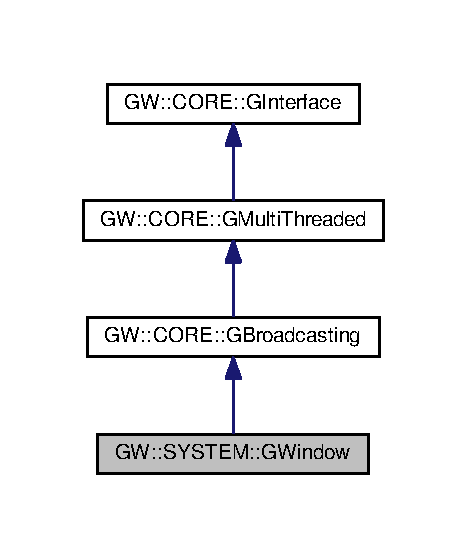
\includegraphics[width=224pt]{classGW_1_1SYSTEM_1_1GWindow__inherit__graph}
\end{center}
\end{figure}


Collaboration diagram for GW\+:\+:S\+Y\+S\+T\+EM\+:\+:G\+Window\+:
\nopagebreak
\begin{figure}[H]
\begin{center}
\leavevmode
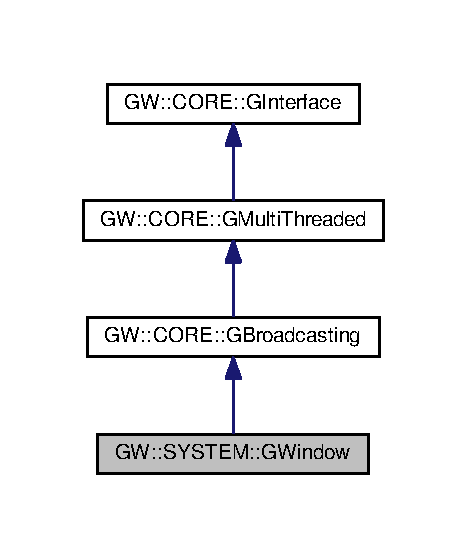
\includegraphics[width=224pt]{classGW_1_1SYSTEM_1_1GWindow__coll__graph}
\end{center}
\end{figure}
\subsection*{Public Member Functions}
\begin{DoxyCompactItemize}
\item 
virtual \hyperlink{namespaceGW_a67a839e3df7ea8a5c5686613a7a3de21}{G\+Return} \hyperlink{classGW_1_1SYSTEM_1_1GWindow_a402b550212d77f19638ef1a1db9ad397}{Open\+Window} ()=0
\begin{DoxyCompactList}\small\item\em Initializes a window handle and displays a window. \end{DoxyCompactList}\item 
virtual \hyperlink{namespaceGW_a67a839e3df7ea8a5c5686613a7a3de21}{G\+Return} \hyperlink{classGW_1_1SYSTEM_1_1GWindow_a6c7db60db04436ac21cba3147f287e84}{Process\+Window\+Events} ()=0
\begin{DoxyCompactList}\small\item\em Flushes and processes all messages from the window\textquotesingle{}s event queue. \end{DoxyCompactList}\item 
virtual \hyperlink{namespaceGW_a67a839e3df7ea8a5c5686613a7a3de21}{G\+Return} \hyperlink{classGW_1_1SYSTEM_1_1GWindow_a113350a164370d30932a0476f00e4ea9}{Reconfigure\+Window} (int \+\_\+x, int \+\_\+y, int \+\_\+width, int \+\_\+height, \hyperlink{namespaceGW_1_1SYSTEM_ad117891e556631f842625c348d36a071}{G\+Window\+Style} \+\_\+style)=0
\begin{DoxyCompactList}\small\item\em Gives the currently opened window the specified size, position and style. \end{DoxyCompactList}\item 
virtual \hyperlink{namespaceGW_a67a839e3df7ea8a5c5686613a7a3de21}{G\+Return} \hyperlink{classGW_1_1SYSTEM_1_1GWindow_a9fc043b893f26c35e6ba965adcc17edb}{Move\+Window} (int \+\_\+x, int \+\_\+y)=0
\begin{DoxyCompactList}\small\item\em Repositions the currently opened window to the specified x and y pixels on screen. \end{DoxyCompactList}\item 
virtual \hyperlink{namespaceGW_a67a839e3df7ea8a5c5686613a7a3de21}{G\+Return} \hyperlink{classGW_1_1SYSTEM_1_1GWindow_a92633707248f32e4c166f27f03690d6d}{Resize\+Window} (int \+\_\+width, int \+\_\+height)=0
\begin{DoxyCompactList}\small\item\em Resizes the currently opened window to the specified width and height. \end{DoxyCompactList}\item 
virtual \hyperlink{namespaceGW_a67a839e3df7ea8a5c5686613a7a3de21}{G\+Return} \hyperlink{classGW_1_1SYSTEM_1_1GWindow_a06b5f092e742baca82a0bfc2cbaef153}{Maximize} ()=0
\begin{DoxyCompactList}\small\item\em Resizes the currently opened window to the native maximum resolution. \end{DoxyCompactList}\item 
virtual \hyperlink{namespaceGW_a67a839e3df7ea8a5c5686613a7a3de21}{G\+Return} \hyperlink{classGW_1_1SYSTEM_1_1GWindow_a2cced61a323dac10535904c3899563d8}{Minimize} ()=0
\begin{DoxyCompactList}\small\item\em Minimizes the currently opened window. \end{DoxyCompactList}\item 
virtual \hyperlink{namespaceGW_a67a839e3df7ea8a5c5686613a7a3de21}{G\+Return} \hyperlink{classGW_1_1SYSTEM_1_1GWindow_a21533c58e920d347c377ebdaa6d2b76f}{Change\+Window\+Style} (\hyperlink{namespaceGW_1_1SYSTEM_ad117891e556631f842625c348d36a071}{G\+Window\+Style} \+\_\+style)=0
\begin{DoxyCompactList}\small\item\em Sets the currently opened window\textquotesingle{}s style to the specified style. \end{DoxyCompactList}\item 
virtual int \hyperlink{classGW_1_1SYSTEM_1_1GWindow_a5afa3ef5f507b1dcb041d57280378e62}{Get\+Width} ()=0
\begin{DoxyCompactList}\small\item\em Returns the width in pixels of the currently opened window. \end{DoxyCompactList}\item 
virtual int \hyperlink{classGW_1_1SYSTEM_1_1GWindow_a159a5aca2f2a77b756591ff29574cdc9}{Get\+Height} ()=0
\begin{DoxyCompactList}\small\item\em Returns the height in pixels of the currently opened window. \end{DoxyCompactList}\item 
virtual int \hyperlink{classGW_1_1SYSTEM_1_1GWindow_a1a4bdd7bb12a39d5bbaae53f1e180d91}{Get\+Client\+Width} ()=0
\begin{DoxyCompactList}\small\item\em Returns the client width in pixels of the currently opened window. \end{DoxyCompactList}\item 
virtual int \hyperlink{classGW_1_1SYSTEM_1_1GWindow_ac0a08847a67fbb588f6a851007f465f0}{Get\+Client\+Height} ()=0
\begin{DoxyCompactList}\small\item\em Returns the client height in pixels of the currently opened window. \end{DoxyCompactList}\item 
virtual int \hyperlink{classGW_1_1SYSTEM_1_1GWindow_a085fd92d1a4f5cb131ca405dc69d28ea}{GetX} ()=0
\begin{DoxyCompactList}\small\item\em Returns the X position in pixels of the currently opened window. \end{DoxyCompactList}\item 
virtual int \hyperlink{classGW_1_1SYSTEM_1_1GWindow_a37525397599eb9fc9fced0fe3a69fc04}{GetY} ()=0
\begin{DoxyCompactList}\small\item\em Returns the Y position in pixels of the currently opened window. \end{DoxyCompactList}\item 
virtual \hyperlink{namespaceGW_a67a839e3df7ea8a5c5686613a7a3de21}{G\+Return} \hyperlink{classGW_1_1SYSTEM_1_1GWindow_ac80bfaba809d5eb54d6a11b11deddeb7}{Get\+Client\+Top\+Left} (unsigned int \&\+\_\+outX, unsigned int \&\+\_\+outY)=0
\begin{DoxyCompactList}\small\item\em Gets the location of the top-\/left pixel of the opened window\textquotesingle{}s client area. \end{DoxyCompactList}\item 
virtual void $\ast$ \hyperlink{classGW_1_1SYSTEM_1_1GWindow_aa3cc3af1805ac9573424f8815420e9c5}{Get\+Window\+Handle} ()=0
\begin{DoxyCompactList}\small\item\em Returns the platform specific window handle to the currently opened window. \end{DoxyCompactList}\item 
virtual bool \hyperlink{classGW_1_1SYSTEM_1_1GWindow_acf85e727f26eeeeb3e006947c45d04a3}{Is\+Fullscreen} ()=0
\begin{DoxyCompactList}\small\item\em Returns a bool specifying whether or not the currently opened window is fullscreen. \end{DoxyCompactList}\end{DoxyCompactItemize}


\subsection{Detailed Description}
A thread-\/safe window creation and management library. 

This library is used to create, move, resize, and destroy a window. Methods exist to query information from the window as well. The window is also a broadcaster, meaning a G\+Listener can be written to receive events from it. 

\subsection{Member Function Documentation}
\index{G\+W\+::\+S\+Y\+S\+T\+E\+M\+::\+G\+Window@{G\+W\+::\+S\+Y\+S\+T\+E\+M\+::\+G\+Window}!Change\+Window\+Style@{Change\+Window\+Style}}
\index{Change\+Window\+Style@{Change\+Window\+Style}!G\+W\+::\+S\+Y\+S\+T\+E\+M\+::\+G\+Window@{G\+W\+::\+S\+Y\+S\+T\+E\+M\+::\+G\+Window}}
\subsubsection[{\texorpdfstring{Change\+Window\+Style(\+G\+Window\+Style \+\_\+style)=0}{ChangeWindowStyle(GWindowStyle _style)=0}}]{\setlength{\rightskip}{0pt plus 5cm}virtual {\bf G\+Return} G\+W\+::\+S\+Y\+S\+T\+E\+M\+::\+G\+Window\+::\+Change\+Window\+Style (
\begin{DoxyParamCaption}
\item[{{\bf G\+Window\+Style}}]{\+\_\+style}
\end{DoxyParamCaption}
)\hspace{0.3cm}{\ttfamily [pure virtual]}}\hypertarget{classGW_1_1SYSTEM_1_1GWindow_a21533c58e920d347c377ebdaa6d2b76f}{}\label{classGW_1_1SYSTEM_1_1GWindow_a21533c58e920d347c377ebdaa6d2b76f}


Sets the currently opened window\textquotesingle{}s style to the specified style. 

G\+Window\+Style will be overwritten and the window resized or moved accordingly.


\begin{DoxyParams}[1]{Parameters}
\mbox{\tt in}  & {\em \+\_\+style} & The G\+Window\+Style to change the window to.\\
\hline
\end{DoxyParams}

\begin{DoxyRetVals}{Return values}
{\em S\+U\+C\+C\+E\+SS} & The window style was successfully changed. \\
\hline
{\em R\+E\+D\+U\+N\+D\+A\+N\+T\+\_\+\+O\+P\+E\+R\+A\+T\+I\+ON} & No window exists to change. \\
\hline
\end{DoxyRetVals}
\index{G\+W\+::\+S\+Y\+S\+T\+E\+M\+::\+G\+Window@{G\+W\+::\+S\+Y\+S\+T\+E\+M\+::\+G\+Window}!Get\+Client\+Height@{Get\+Client\+Height}}
\index{Get\+Client\+Height@{Get\+Client\+Height}!G\+W\+::\+S\+Y\+S\+T\+E\+M\+::\+G\+Window@{G\+W\+::\+S\+Y\+S\+T\+E\+M\+::\+G\+Window}}
\subsubsection[{\texorpdfstring{Get\+Client\+Height()=0}{GetClientHeight()=0}}]{\setlength{\rightskip}{0pt plus 5cm}virtual int G\+W\+::\+S\+Y\+S\+T\+E\+M\+::\+G\+Window\+::\+Get\+Client\+Height (
\begin{DoxyParamCaption}
{}
\end{DoxyParamCaption}
)\hspace{0.3cm}{\ttfamily [pure virtual]}}\hypertarget{classGW_1_1SYSTEM_1_1GWindow_ac0a08847a67fbb588f6a851007f465f0}{}\label{classGW_1_1SYSTEM_1_1GWindow_ac0a08847a67fbb588f6a851007f465f0}


Returns the client height in pixels of the currently opened window. 


\begin{DoxyRetVals}{Return values}
{\em 0} & The window is minimized. \\
\hline
{\em -\/1} & No window exists to query size from. \\
\hline
{\em else} & Height was successfully queried and returned. \\
\hline
\end{DoxyRetVals}
\index{G\+W\+::\+S\+Y\+S\+T\+E\+M\+::\+G\+Window@{G\+W\+::\+S\+Y\+S\+T\+E\+M\+::\+G\+Window}!Get\+Client\+Top\+Left@{Get\+Client\+Top\+Left}}
\index{Get\+Client\+Top\+Left@{Get\+Client\+Top\+Left}!G\+W\+::\+S\+Y\+S\+T\+E\+M\+::\+G\+Window@{G\+W\+::\+S\+Y\+S\+T\+E\+M\+::\+G\+Window}}
\subsubsection[{\texorpdfstring{Get\+Client\+Top\+Left(unsigned int \&\+\_\+out\+X, unsigned int \&\+\_\+out\+Y)=0}{GetClientTopLeft(unsigned int &_outX, unsigned int &_outY)=0}}]{\setlength{\rightskip}{0pt plus 5cm}virtual {\bf G\+Return} G\+W\+::\+S\+Y\+S\+T\+E\+M\+::\+G\+Window\+::\+Get\+Client\+Top\+Left (
\begin{DoxyParamCaption}
\item[{unsigned int \&}]{\+\_\+outX, }
\item[{unsigned int \&}]{\+\_\+outY}
\end{DoxyParamCaption}
)\hspace{0.3cm}{\ttfamily [pure virtual]}}\hypertarget{classGW_1_1SYSTEM_1_1GWindow_ac80bfaba809d5eb54d6a11b11deddeb7}{}\label{classGW_1_1SYSTEM_1_1GWindow_ac80bfaba809d5eb54d6a11b11deddeb7}


Gets the location of the top-\/left pixel of the opened window\textquotesingle{}s client area. 


\begin{DoxyParams}[1]{Parameters}
\mbox{\tt out}  & {\em \+\_\+outX} & Will contain the X location of the top-\/left pixel. \\
\hline
\mbox{\tt out}  & {\em \+\_\+outY} & Will contain the Y location of the top-\/left pixel.\\
\hline
\end{DoxyParams}

\begin{DoxyRetVals}{Return values}
{\em -\/1} & No window exists to query position from. \\
\hline
{\em else} & Position was successfully queried and returned. \\
\hline
\end{DoxyRetVals}
\index{G\+W\+::\+S\+Y\+S\+T\+E\+M\+::\+G\+Window@{G\+W\+::\+S\+Y\+S\+T\+E\+M\+::\+G\+Window}!Get\+Client\+Width@{Get\+Client\+Width}}
\index{Get\+Client\+Width@{Get\+Client\+Width}!G\+W\+::\+S\+Y\+S\+T\+E\+M\+::\+G\+Window@{G\+W\+::\+S\+Y\+S\+T\+E\+M\+::\+G\+Window}}
\subsubsection[{\texorpdfstring{Get\+Client\+Width()=0}{GetClientWidth()=0}}]{\setlength{\rightskip}{0pt plus 5cm}virtual int G\+W\+::\+S\+Y\+S\+T\+E\+M\+::\+G\+Window\+::\+Get\+Client\+Width (
\begin{DoxyParamCaption}
{}
\end{DoxyParamCaption}
)\hspace{0.3cm}{\ttfamily [pure virtual]}}\hypertarget{classGW_1_1SYSTEM_1_1GWindow_a1a4bdd7bb12a39d5bbaae53f1e180d91}{}\label{classGW_1_1SYSTEM_1_1GWindow_a1a4bdd7bb12a39d5bbaae53f1e180d91}


Returns the client width in pixels of the currently opened window. 

Client height is the height of the window\textquotesingle{}s drawable area.


\begin{DoxyRetVals}{Return values}
{\em 0} & The window is minimized. \\
\hline
{\em -\/1} & No window exists to query size from. \\
\hline
{\em else} & Width was successfully queried and returned. \\
\hline
\end{DoxyRetVals}
\index{G\+W\+::\+S\+Y\+S\+T\+E\+M\+::\+G\+Window@{G\+W\+::\+S\+Y\+S\+T\+E\+M\+::\+G\+Window}!Get\+Height@{Get\+Height}}
\index{Get\+Height@{Get\+Height}!G\+W\+::\+S\+Y\+S\+T\+E\+M\+::\+G\+Window@{G\+W\+::\+S\+Y\+S\+T\+E\+M\+::\+G\+Window}}
\subsubsection[{\texorpdfstring{Get\+Height()=0}{GetHeight()=0}}]{\setlength{\rightskip}{0pt plus 5cm}virtual int G\+W\+::\+S\+Y\+S\+T\+E\+M\+::\+G\+Window\+::\+Get\+Height (
\begin{DoxyParamCaption}
{}
\end{DoxyParamCaption}
)\hspace{0.3cm}{\ttfamily [pure virtual]}}\hypertarget{classGW_1_1SYSTEM_1_1GWindow_a159a5aca2f2a77b756591ff29574cdc9}{}\label{classGW_1_1SYSTEM_1_1GWindow_a159a5aca2f2a77b756591ff29574cdc9}


Returns the height in pixels of the currently opened window. 

Client width is the width of the window\textquotesingle{}s drawable area.


\begin{DoxyRetVals}{Return values}
{\em 0} & The window is minimized. \\
\hline
{\em -\/1} & No window exists to query size from. \\
\hline
{\em else} & Height was successfully queried and returned. \\
\hline
\end{DoxyRetVals}
\index{G\+W\+::\+S\+Y\+S\+T\+E\+M\+::\+G\+Window@{G\+W\+::\+S\+Y\+S\+T\+E\+M\+::\+G\+Window}!Get\+Width@{Get\+Width}}
\index{Get\+Width@{Get\+Width}!G\+W\+::\+S\+Y\+S\+T\+E\+M\+::\+G\+Window@{G\+W\+::\+S\+Y\+S\+T\+E\+M\+::\+G\+Window}}
\subsubsection[{\texorpdfstring{Get\+Width()=0}{GetWidth()=0}}]{\setlength{\rightskip}{0pt plus 5cm}virtual int G\+W\+::\+S\+Y\+S\+T\+E\+M\+::\+G\+Window\+::\+Get\+Width (
\begin{DoxyParamCaption}
{}
\end{DoxyParamCaption}
)\hspace{0.3cm}{\ttfamily [pure virtual]}}\hypertarget{classGW_1_1SYSTEM_1_1GWindow_a5afa3ef5f507b1dcb041d57280378e62}{}\label{classGW_1_1SYSTEM_1_1GWindow_a5afa3ef5f507b1dcb041d57280378e62}


Returns the width in pixels of the currently opened window. 


\begin{DoxyRetVals}{Return values}
{\em 0} & The window is minimized. \\
\hline
{\em -\/1} & No window exists to query size from. \\
\hline
{\em else} & Width was successfully queried and returned. \\
\hline
\end{DoxyRetVals}
\index{G\+W\+::\+S\+Y\+S\+T\+E\+M\+::\+G\+Window@{G\+W\+::\+S\+Y\+S\+T\+E\+M\+::\+G\+Window}!Get\+Window\+Handle@{Get\+Window\+Handle}}
\index{Get\+Window\+Handle@{Get\+Window\+Handle}!G\+W\+::\+S\+Y\+S\+T\+E\+M\+::\+G\+Window@{G\+W\+::\+S\+Y\+S\+T\+E\+M\+::\+G\+Window}}
\subsubsection[{\texorpdfstring{Get\+Window\+Handle()=0}{GetWindowHandle()=0}}]{\setlength{\rightskip}{0pt plus 5cm}virtual void$\ast$ G\+W\+::\+S\+Y\+S\+T\+E\+M\+::\+G\+Window\+::\+Get\+Window\+Handle (
\begin{DoxyParamCaption}
{}
\end{DoxyParamCaption}
)\hspace{0.3cm}{\ttfamily [pure virtual]}}\hypertarget{classGW_1_1SYSTEM_1_1GWindow_aa3cc3af1805ac9573424f8815420e9c5}{}\label{classGW_1_1SYSTEM_1_1GWindow_aa3cc3af1805ac9573424f8815420e9c5}


Returns the platform specific window handle to the currently opened window. 

On Windows the void$\ast$ is an H\+W\+ND, on Linux a \hyperlink{structGW_1_1SYSTEM_1_1LINUX__WINDOW}{L\+I\+N\+U\+X\+\_\+\+W\+I\+N\+D\+OW}, and on Mac an N\+S\+Window. Methods exist to query window information right from these handles.


\begin{DoxyRetVals}{Return values}
{\em void$\ast$} & The void$\ast$ data to the window handle. \\
\hline
\end{DoxyRetVals}
\index{G\+W\+::\+S\+Y\+S\+T\+E\+M\+::\+G\+Window@{G\+W\+::\+S\+Y\+S\+T\+E\+M\+::\+G\+Window}!GetX@{GetX}}
\index{GetX@{GetX}!G\+W\+::\+S\+Y\+S\+T\+E\+M\+::\+G\+Window@{G\+W\+::\+S\+Y\+S\+T\+E\+M\+::\+G\+Window}}
\subsubsection[{\texorpdfstring{Get\+X()=0}{GetX()=0}}]{\setlength{\rightskip}{0pt plus 5cm}virtual int G\+W\+::\+S\+Y\+S\+T\+E\+M\+::\+G\+Window\+::\+GetX (
\begin{DoxyParamCaption}
{}
\end{DoxyParamCaption}
)\hspace{0.3cm}{\ttfamily [pure virtual]}}\hypertarget{classGW_1_1SYSTEM_1_1GWindow_a085fd92d1a4f5cb131ca405dc69d28ea}{}\label{classGW_1_1SYSTEM_1_1GWindow_a085fd92d1a4f5cb131ca405dc69d28ea}


Returns the X position in pixels of the currently opened window. 


\begin{DoxyRetVals}{Return values}
{\em -\/1} & No window exists to query position from. \\
\hline
{\em else} & X position was successfully queried and returned. \\
\hline
\end{DoxyRetVals}
\index{G\+W\+::\+S\+Y\+S\+T\+E\+M\+::\+G\+Window@{G\+W\+::\+S\+Y\+S\+T\+E\+M\+::\+G\+Window}!GetY@{GetY}}
\index{GetY@{GetY}!G\+W\+::\+S\+Y\+S\+T\+E\+M\+::\+G\+Window@{G\+W\+::\+S\+Y\+S\+T\+E\+M\+::\+G\+Window}}
\subsubsection[{\texorpdfstring{Get\+Y()=0}{GetY()=0}}]{\setlength{\rightskip}{0pt plus 5cm}virtual int G\+W\+::\+S\+Y\+S\+T\+E\+M\+::\+G\+Window\+::\+GetY (
\begin{DoxyParamCaption}
{}
\end{DoxyParamCaption}
)\hspace{0.3cm}{\ttfamily [pure virtual]}}\hypertarget{classGW_1_1SYSTEM_1_1GWindow_a37525397599eb9fc9fced0fe3a69fc04}{}\label{classGW_1_1SYSTEM_1_1GWindow_a37525397599eb9fc9fced0fe3a69fc04}


Returns the Y position in pixels of the currently opened window. 


\begin{DoxyRetVals}{Return values}
{\em -\/1} & No window exists to query position from. \\
\hline
{\em else} & Y position was successfully queried and returned. \\
\hline
\end{DoxyRetVals}
\index{G\+W\+::\+S\+Y\+S\+T\+E\+M\+::\+G\+Window@{G\+W\+::\+S\+Y\+S\+T\+E\+M\+::\+G\+Window}!Is\+Fullscreen@{Is\+Fullscreen}}
\index{Is\+Fullscreen@{Is\+Fullscreen}!G\+W\+::\+S\+Y\+S\+T\+E\+M\+::\+G\+Window@{G\+W\+::\+S\+Y\+S\+T\+E\+M\+::\+G\+Window}}
\subsubsection[{\texorpdfstring{Is\+Fullscreen()=0}{IsFullscreen()=0}}]{\setlength{\rightskip}{0pt plus 5cm}virtual bool G\+W\+::\+S\+Y\+S\+T\+E\+M\+::\+G\+Window\+::\+Is\+Fullscreen (
\begin{DoxyParamCaption}
{}
\end{DoxyParamCaption}
)\hspace{0.3cm}{\ttfamily [pure virtual]}}\hypertarget{classGW_1_1SYSTEM_1_1GWindow_acf85e727f26eeeeb3e006947c45d04a3}{}\label{classGW_1_1SYSTEM_1_1GWindow_acf85e727f26eeeeb3e006947c45d04a3}


Returns a bool specifying whether or not the currently opened window is fullscreen. 


\begin{DoxyRetVals}{Return values}
{\em true} & The window is fullscreen. \\
\hline
{\em false} & The window is not fullscreen. \\
\hline
\end{DoxyRetVals}
\index{G\+W\+::\+S\+Y\+S\+T\+E\+M\+::\+G\+Window@{G\+W\+::\+S\+Y\+S\+T\+E\+M\+::\+G\+Window}!Maximize@{Maximize}}
\index{Maximize@{Maximize}!G\+W\+::\+S\+Y\+S\+T\+E\+M\+::\+G\+Window@{G\+W\+::\+S\+Y\+S\+T\+E\+M\+::\+G\+Window}}
\subsubsection[{\texorpdfstring{Maximize()=0}{Maximize()=0}}]{\setlength{\rightskip}{0pt plus 5cm}virtual {\bf G\+Return} G\+W\+::\+S\+Y\+S\+T\+E\+M\+::\+G\+Window\+::\+Maximize (
\begin{DoxyParamCaption}
{}
\end{DoxyParamCaption}
)\hspace{0.3cm}{\ttfamily [pure virtual]}}\hypertarget{classGW_1_1SYSTEM_1_1GWindow_a06b5f092e742baca82a0bfc2cbaef153}{}\label{classGW_1_1SYSTEM_1_1GWindow_a06b5f092e742baca82a0bfc2cbaef153}


Resizes the currently opened window to the native maximum resolution. 

G\+Window\+Style will be overwritten to be the fullscreen version if it is not already.


\begin{DoxyRetVals}{Return values}
{\em S\+U\+C\+C\+E\+SS} & The window was successfully maximized. \\
\hline
{\em R\+E\+D\+U\+N\+D\+A\+N\+T\+\_\+\+O\+P\+E\+R\+A\+T\+I\+ON} & No window exists to maximize. \\
\hline
\end{DoxyRetVals}
\index{G\+W\+::\+S\+Y\+S\+T\+E\+M\+::\+G\+Window@{G\+W\+::\+S\+Y\+S\+T\+E\+M\+::\+G\+Window}!Minimize@{Minimize}}
\index{Minimize@{Minimize}!G\+W\+::\+S\+Y\+S\+T\+E\+M\+::\+G\+Window@{G\+W\+::\+S\+Y\+S\+T\+E\+M\+::\+G\+Window}}
\subsubsection[{\texorpdfstring{Minimize()=0}{Minimize()=0}}]{\setlength{\rightskip}{0pt plus 5cm}virtual {\bf G\+Return} G\+W\+::\+S\+Y\+S\+T\+E\+M\+::\+G\+Window\+::\+Minimize (
\begin{DoxyParamCaption}
{}
\end{DoxyParamCaption}
)\hspace{0.3cm}{\ttfamily [pure virtual]}}\hypertarget{classGW_1_1SYSTEM_1_1GWindow_a2cced61a323dac10535904c3899563d8}{}\label{classGW_1_1SYSTEM_1_1GWindow_a2cced61a323dac10535904c3899563d8}


Minimizes the currently opened window. 

G\+Window\+Style will be overwritten to be the minimized style if it is not already.


\begin{DoxyRetVals}{Return values}
{\em S\+U\+C\+C\+E\+SS} & The window was successfully minimized. \\
\hline
{\em R\+E\+D\+U\+N\+D\+A\+N\+T\+\_\+\+O\+P\+E\+R\+A\+T\+I\+ON} & No window exists to minimize or window is already maximized. \\
\hline
\end{DoxyRetVals}
\index{G\+W\+::\+S\+Y\+S\+T\+E\+M\+::\+G\+Window@{G\+W\+::\+S\+Y\+S\+T\+E\+M\+::\+G\+Window}!Move\+Window@{Move\+Window}}
\index{Move\+Window@{Move\+Window}!G\+W\+::\+S\+Y\+S\+T\+E\+M\+::\+G\+Window@{G\+W\+::\+S\+Y\+S\+T\+E\+M\+::\+G\+Window}}
\subsubsection[{\texorpdfstring{Move\+Window(int \+\_\+x, int \+\_\+y)=0}{MoveWindow(int _x, int _y)=0}}]{\setlength{\rightskip}{0pt plus 5cm}virtual {\bf G\+Return} G\+W\+::\+S\+Y\+S\+T\+E\+M\+::\+G\+Window\+::\+Move\+Window (
\begin{DoxyParamCaption}
\item[{int}]{\+\_\+x, }
\item[{int}]{\+\_\+y}
\end{DoxyParamCaption}
)\hspace{0.3cm}{\ttfamily [pure virtual]}}\hypertarget{classGW_1_1SYSTEM_1_1GWindow_a9fc043b893f26c35e6ba965adcc17edb}{}\label{classGW_1_1SYSTEM_1_1GWindow_a9fc043b893f26c35e6ba965adcc17edb}


Repositions the currently opened window to the specified x and y pixels on screen. 

If position parameters are less than 0 then 0 will be used. If position parameters are greater than native resoultion, maximum native resolution parameters will be used.


\begin{DoxyParams}[1]{Parameters}
\mbox{\tt in}  & {\em \+\_\+x} & The x position on screen to move the window to. \\
\hline
\mbox{\tt in}  & {\em \+\_\+y} & The y position on screen to move the window to.\\
\hline
\end{DoxyParams}

\begin{DoxyRetVals}{Return values}
{\em S\+U\+C\+C\+E\+SS} & The window was successfully moved. \\
\hline
{\em I\+N\+V\+A\+L\+I\+D\+\_\+\+A\+R\+G\+U\+M\+E\+NT} & The style passed in is invalid \\
\hline
{\em R\+E\+D\+U\+N\+D\+A\+N\+T\+\_\+\+O\+P\+E\+R\+A\+T\+I\+ON} & No window exists to move. \\
\hline
\end{DoxyRetVals}
\index{G\+W\+::\+S\+Y\+S\+T\+E\+M\+::\+G\+Window@{G\+W\+::\+S\+Y\+S\+T\+E\+M\+::\+G\+Window}!Open\+Window@{Open\+Window}}
\index{Open\+Window@{Open\+Window}!G\+W\+::\+S\+Y\+S\+T\+E\+M\+::\+G\+Window@{G\+W\+::\+S\+Y\+S\+T\+E\+M\+::\+G\+Window}}
\subsubsection[{\texorpdfstring{Open\+Window()=0}{OpenWindow()=0}}]{\setlength{\rightskip}{0pt plus 5cm}virtual {\bf G\+Return} G\+W\+::\+S\+Y\+S\+T\+E\+M\+::\+G\+Window\+::\+Open\+Window (
\begin{DoxyParamCaption}
{}
\end{DoxyParamCaption}
)\hspace{0.3cm}{\ttfamily [pure virtual]}}\hypertarget{classGW_1_1SYSTEM_1_1GWindow_a402b550212d77f19638ef1a1db9ad397}{}\label{classGW_1_1SYSTEM_1_1GWindow_a402b550212d77f19638ef1a1db9ad397}


Initializes a window handle and displays a window. 

The window is opened with the size, position and style specified in the parameters passed into the Create\+G\+Window function. Parameters were checked for invalid values during the initialization of the window after creation, so it is assumed the window has valid parameters before this function is called.


\begin{DoxyRetVals}{Return values}
{\em S\+U\+C\+C\+E\+SS} & The window was successfully created and displayed. \\
\hline
{\em R\+E\+D\+U\+N\+D\+A\+N\+T\+\_\+\+O\+P\+E\+R\+A\+T\+I\+ON} & The \hyperlink{classGW_1_1SYSTEM_1_1GWindow}{G\+Window} object already has a window open \\
\hline
{\em F\+A\+I\+L\+U\+RE} & The window could not be created. \\
\hline
\end{DoxyRetVals}
\index{G\+W\+::\+S\+Y\+S\+T\+E\+M\+::\+G\+Window@{G\+W\+::\+S\+Y\+S\+T\+E\+M\+::\+G\+Window}!Process\+Window\+Events@{Process\+Window\+Events}}
\index{Process\+Window\+Events@{Process\+Window\+Events}!G\+W\+::\+S\+Y\+S\+T\+E\+M\+::\+G\+Window@{G\+W\+::\+S\+Y\+S\+T\+E\+M\+::\+G\+Window}}
\subsubsection[{\texorpdfstring{Process\+Window\+Events()=0}{ProcessWindowEvents()=0}}]{\setlength{\rightskip}{0pt plus 5cm}virtual {\bf G\+Return} G\+W\+::\+S\+Y\+S\+T\+E\+M\+::\+G\+Window\+::\+Process\+Window\+Events (
\begin{DoxyParamCaption}
{}
\end{DoxyParamCaption}
)\hspace{0.3cm}{\ttfamily [pure virtual]}}\hypertarget{classGW_1_1SYSTEM_1_1GWindow_a6c7db60db04436ac21cba3147f287e84}{}\label{classGW_1_1SYSTEM_1_1GWindow_a6c7db60db04436ac21cba3147f287e84}


Flushes and processes all messages from the window\textquotesingle{}s event queue. 

This function is meant to be called once a frame in an application\textquotesingle{}s main loop. This function will break when all waiting messages have been processed and the event queue is empty.


\begin{DoxyRetVals}{Return values}
{\em S\+U\+C\+C\+E\+SS} & The messages were successfully processed and removed. \\
\hline
{\em R\+E\+D\+U\+N\+D\+A\+N\+T\+\_\+\+O\+P\+E\+R\+A\+T\+I\+ON} & No window exists process. \\
\hline
\end{DoxyRetVals}
\index{G\+W\+::\+S\+Y\+S\+T\+E\+M\+::\+G\+Window@{G\+W\+::\+S\+Y\+S\+T\+E\+M\+::\+G\+Window}!Reconfigure\+Window@{Reconfigure\+Window}}
\index{Reconfigure\+Window@{Reconfigure\+Window}!G\+W\+::\+S\+Y\+S\+T\+E\+M\+::\+G\+Window@{G\+W\+::\+S\+Y\+S\+T\+E\+M\+::\+G\+Window}}
\subsubsection[{\texorpdfstring{Reconfigure\+Window(int \+\_\+x, int \+\_\+y, int \+\_\+width, int \+\_\+height, G\+Window\+Style \+\_\+style)=0}{ReconfigureWindow(int _x, int _y, int _width, int _height, GWindowStyle _style)=0}}]{\setlength{\rightskip}{0pt plus 5cm}virtual {\bf G\+Return} G\+W\+::\+S\+Y\+S\+T\+E\+M\+::\+G\+Window\+::\+Reconfigure\+Window (
\begin{DoxyParamCaption}
\item[{int}]{\+\_\+x, }
\item[{int}]{\+\_\+y, }
\item[{int}]{\+\_\+width, }
\item[{int}]{\+\_\+height, }
\item[{{\bf G\+Window\+Style}}]{\+\_\+style}
\end{DoxyParamCaption}
)\hspace{0.3cm}{\ttfamily [pure virtual]}}\hypertarget{classGW_1_1SYSTEM_1_1GWindow_a113350a164370d30932a0476f00e4ea9}{}\label{classGW_1_1SYSTEM_1_1GWindow_a113350a164370d30932a0476f00e4ea9}


Gives the currently opened window the specified size, position and style. 

If width and height are equal to or greater than the native resolution, the passed in G\+Window\+Style will be overwritten to be the fullscreen version if it is not already. If position parameters are less than 0 then 0 will be used. If position parameters are greater than native resoultion, maximum native resolution parameters will be used.


\begin{DoxyParams}[1]{Parameters}
\mbox{\tt in}  & {\em \+\_\+x} & The x position on screen to move the window to. \\
\hline
\mbox{\tt in}  & {\em \+\_\+y} & The y position on screen to move the window to. \\
\hline
\mbox{\tt in}  & {\em \+\_\+width} & The width to give the window. \\
\hline
\mbox{\tt in}  & {\em \+\_\+height} & The height to give the window. \\
\hline
\mbox{\tt in}  & {\em \+\_\+style} & The style to give to the window. (see G\+Window\+Style for style options)\\
\hline
\end{DoxyParams}

\begin{DoxyRetVals}{Return values}
{\em S\+U\+C\+C\+E\+SS} & The window successfully had its attributes changed. \\
\hline
{\em I\+N\+V\+A\+L\+I\+D\+\_\+\+A\+R\+G\+U\+M\+E\+NT} & One of the size parameters are outside the limits of the hardware. \\
\hline
{\em R\+E\+D\+U\+N\+D\+A\+N\+T\+\_\+\+O\+P\+E\+R\+A\+T\+I\+ON} & No window exists to edit. \\
\hline
\end{DoxyRetVals}
\index{G\+W\+::\+S\+Y\+S\+T\+E\+M\+::\+G\+Window@{G\+W\+::\+S\+Y\+S\+T\+E\+M\+::\+G\+Window}!Resize\+Window@{Resize\+Window}}
\index{Resize\+Window@{Resize\+Window}!G\+W\+::\+S\+Y\+S\+T\+E\+M\+::\+G\+Window@{G\+W\+::\+S\+Y\+S\+T\+E\+M\+::\+G\+Window}}
\subsubsection[{\texorpdfstring{Resize\+Window(int \+\_\+width, int \+\_\+height)=0}{ResizeWindow(int _width, int _height)=0}}]{\setlength{\rightskip}{0pt plus 5cm}virtual {\bf G\+Return} G\+W\+::\+S\+Y\+S\+T\+E\+M\+::\+G\+Window\+::\+Resize\+Window (
\begin{DoxyParamCaption}
\item[{int}]{\+\_\+width, }
\item[{int}]{\+\_\+height}
\end{DoxyParamCaption}
)\hspace{0.3cm}{\ttfamily [pure virtual]}}\hypertarget{classGW_1_1SYSTEM_1_1GWindow_a92633707248f32e4c166f27f03690d6d}{}\label{classGW_1_1SYSTEM_1_1GWindow_a92633707248f32e4c166f27f03690d6d}


Resizes the currently opened window to the specified width and height. 

If width and height are greater than the native resolution, the G\+Window\+Style will be overwritten to be the fullscreen version if it is not already. If position parameters are less than 0 then 0 will be used. If position parameters are greater than native resoultion, maximum native resolution parameters will be used.


\begin{DoxyParams}[1]{Parameters}
\mbox{\tt in}  & {\em \+\_\+x} & The width to resize the window to. \\
\hline
\mbox{\tt in}  & {\em \+\_\+y} & The height to resize the window to.\\
\hline
\end{DoxyParams}

\begin{DoxyRetVals}{Return values}
{\em S\+U\+C\+C\+E\+SS} & The window was successfully resized. \\
\hline
{\em I\+N\+V\+A\+L\+I\+D\+\_\+\+A\+R\+G\+U\+M\+E\+NT} & One of the size parameters are less than or equal to 0. \\
\hline
{\em R\+E\+D\+U\+N\+D\+A\+N\+T\+\_\+\+O\+P\+E\+R\+A\+T\+I\+ON} & No window exists to resize. \\
\hline
\end{DoxyRetVals}


The documentation for this class was generated from the following file\+:\begin{DoxyCompactItemize}
\item 
Interface/\+G\+\_\+\+System/G\+Window.\+h\end{DoxyCompactItemize}

\hypertarget{structGW_1_1SYSTEM_1_1GWINDOW__EVENT__DATA}{}\section{GW\+::S\+Y\+S\+T\+EM\+::G\+W\+I\+N\+D\+O\+W\+\_\+\+E\+V\+E\+N\+T\+\_\+\+D\+A\+TA Struct Reference}
\label{structGW_1_1SYSTEM_1_1GWINDOW__EVENT__DATA}\index{GW::SYSTEM::GWINDOW\_EVENT\_DATA@{GW::SYSTEM::GWINDOW\_EVENT\_DATA}}


Ensure identical binary padding for structures on all platforms.  




{\ttfamily \#include $<$G\+Window.\+h$>$}

\subsection*{Public Attributes}
\begin{DoxyCompactItemize}
\item 
\mbox{\Hypertarget{structGW_1_1SYSTEM_1_1GWINDOW__EVENT__DATA_a9a3463e7fe90f6c9cb4c4f7d68f62ee1}\label{structGW_1_1SYSTEM_1_1GWINDOW__EVENT__DATA_a9a3463e7fe90f6c9cb4c4f7d68f62ee1}} 
unsigned int {\bfseries event\+Flags}
\item 
\mbox{\Hypertarget{structGW_1_1SYSTEM_1_1GWINDOW__EVENT__DATA_a1bd478c20e20d67fcef4278888f29225}\label{structGW_1_1SYSTEM_1_1GWINDOW__EVENT__DATA_a1bd478c20e20d67fcef4278888f29225}} 
unsigned int {\bfseries height}
\item 
\mbox{\Hypertarget{structGW_1_1SYSTEM_1_1GWINDOW__EVENT__DATA_aedd64cb9564e161fc24a9ea597576dc9}\label{structGW_1_1SYSTEM_1_1GWINDOW__EVENT__DATA_aedd64cb9564e161fc24a9ea597576dc9}} 
unsigned int {\bfseries width}
\item 
\mbox{\Hypertarget{structGW_1_1SYSTEM_1_1GWINDOW__EVENT__DATA_acb671b49c59e58b84d797e5c3ac6deaf}\label{structGW_1_1SYSTEM_1_1GWINDOW__EVENT__DATA_acb671b49c59e58b84d797e5c3ac6deaf}} 
int {\bfseries windowX}
\item 
\mbox{\Hypertarget{structGW_1_1SYSTEM_1_1GWINDOW__EVENT__DATA_aaf455dc933271e4ba81225b8b0433ebc}\label{structGW_1_1SYSTEM_1_1GWINDOW__EVENT__DATA_aaf455dc933271e4ba81225b8b0433ebc}} 
int {\bfseries windowY}
\item 
\mbox{\Hypertarget{structGW_1_1SYSTEM_1_1GWINDOW__EVENT__DATA_a08f52d27570c3cad613dd19fe72a88ac}\label{structGW_1_1SYSTEM_1_1GWINDOW__EVENT__DATA_a08f52d27570c3cad613dd19fe72a88ac}} 
void $\ast$ {\bfseries window\+Handle}
\end{DoxyCompactItemize}


\subsection{Detailed Description}
Ensure identical binary padding for structures on all platforms. 

The documentation for this struct was generated from the following file\+:\begin{DoxyCompactItemize}
\item 
Interface/\+G\+\_\+\+System/G\+Window.\+h\end{DoxyCompactItemize}

\hypertarget{classGWindowTestListener}{}\section{G\+Window\+Test\+Listener Class Reference}
\label{classGWindowTestListener}\index{G\+Window\+Test\+Listener@{G\+Window\+Test\+Listener}}


Inheritance diagram for G\+Window\+Test\+Listener\+:
\nopagebreak
\begin{figure}[H]
\begin{center}
\leavevmode
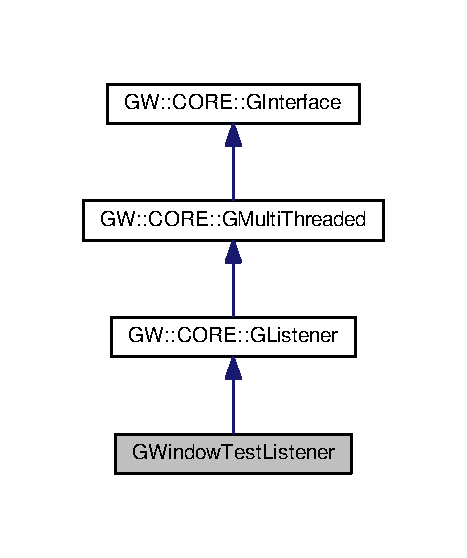
\includegraphics[width=224pt]{classGWindowTestListener__inherit__graph}
\end{center}
\end{figure}


Collaboration diagram for G\+Window\+Test\+Listener\+:
\nopagebreak
\begin{figure}[H]
\begin{center}
\leavevmode
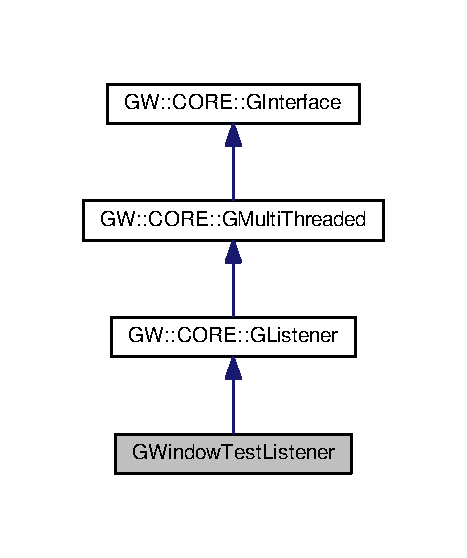
\includegraphics[width=224pt]{classGWindowTestListener__coll__graph}
\end{center}
\end{figure}
\subsection*{Public Member Functions}
\begin{DoxyCompactItemize}
\item 
\hyperlink{namespaceGW_a67a839e3df7ea8a5c5686613a7a3de21}{G\+W\+::\+G\+Return} \hyperlink{classGWindowTestListener_a4033e5d1546bbf9fea0cc8062fb31423}{On\+Event} (const \hyperlink{structGW_1_1GUUIID}{G\+W\+::\+G\+U\+U\+I\+ID} \&\+\_\+sender\+Interface, unsigned int \+\_\+event\+ID, void $\ast$\+\_\+event\+Data, unsigned int \+\_\+size\+Of\+Data)
\begin{DoxyCompactList}\small\item\em This operation is called whenever a G\+Broadcaster a listener is registered to generates an event. \end{DoxyCompactList}\item 
\hyperlink{namespaceGW_a67a839e3df7ea8a5c5686613a7a3de21}{G\+W\+::\+G\+Return} \hyperlink{classGWindowTestListener_ab32d49a0521eae89c76337ff9796dc53}{Get\+Count} (unsigned int \&\+\_\+out\+Count)
\begin{DoxyCompactList}\small\item\em Return the total number of active references to this object. \end{DoxyCompactList}\item 
\hyperlink{namespaceGW_a67a839e3df7ea8a5c5686613a7a3de21}{G\+W\+::\+G\+Return} \hyperlink{classGWindowTestListener_a8a4d37e640f882b116bba8f76675c81a}{Increment\+Count} ()
\begin{DoxyCompactList}\small\item\em Increase the total number of active references to this object. \end{DoxyCompactList}\item 
\hyperlink{namespaceGW_a67a839e3df7ea8a5c5686613a7a3de21}{G\+W\+::\+G\+Return} \hyperlink{classGWindowTestListener_a4d5884434e75e2ff23edafe5e0608838}{Decrement\+Count} ()
\begin{DoxyCompactList}\small\item\em Decrease the total number of active references to this object. \end{DoxyCompactList}\item 
\hyperlink{namespaceGW_a67a839e3df7ea8a5c5686613a7a3de21}{G\+W\+::\+G\+Return} \hyperlink{classGWindowTestListener_ae73a5d2fb7659d1b7a98d35d068e6e75}{Request\+Interface} (const \hyperlink{structGW_1_1GUUIID}{G\+W\+::\+G\+U\+U\+I\+ID} \&\+\_\+interface\+ID, void $\ast$$\ast$\+\_\+output\+Interface)
\begin{DoxyCompactList}\small\item\em Requests an interface that may or may not be supported by this object. \end{DoxyCompactList}\item 
int {\bfseries Get\+Window\+Test\+Value} ()\hypertarget{classGWindowTestListener_a8c16dd8b8f68ce0311e946ce11669ace}{}\label{classGWindowTestListener_a8c16dd8b8f68ce0311e946ce11669ace}

\end{DoxyCompactItemize}


\subsection{Member Function Documentation}
\index{G\+Window\+Test\+Listener@{G\+Window\+Test\+Listener}!Decrement\+Count@{Decrement\+Count}}
\index{Decrement\+Count@{Decrement\+Count}!G\+Window\+Test\+Listener@{G\+Window\+Test\+Listener}}
\subsubsection[{\texorpdfstring{Decrement\+Count()}{DecrementCount()}}]{\setlength{\rightskip}{0pt plus 5cm}{\bf G\+W\+::\+G\+Return} G\+Window\+Test\+Listener\+::\+Decrement\+Count (
\begin{DoxyParamCaption}
{}
\end{DoxyParamCaption}
)\hspace{0.3cm}{\ttfamily [virtual]}}\hypertarget{classGWindowTestListener_a4d5884434e75e2ff23edafe5e0608838}{}\label{classGWindowTestListener_a4d5884434e75e2ff23edafe5e0608838}


Decrease the total number of active references to this object. 

Once the internal count reaches zero this object will be deallocated and your pointer will become invalid.


\begin{DoxyRetVals}{Return values}
{\em S\+U\+C\+C\+E\+SS} & Successfully decremented the internal reference count. \\
\hline
{\em F\+A\+I\+L\+U\+RE} & Decrementing of internal reference count would underflow the value. \\
\hline
\end{DoxyRetVals}


Implements \hyperlink{classGW_1_1CORE_1_1GInterface_a19a368c77ad0aa7f49b5a4f772f173ba}{G\+W\+::\+C\+O\+R\+E\+::\+G\+Interface}.

\index{G\+Window\+Test\+Listener@{G\+Window\+Test\+Listener}!Get\+Count@{Get\+Count}}
\index{Get\+Count@{Get\+Count}!G\+Window\+Test\+Listener@{G\+Window\+Test\+Listener}}
\subsubsection[{\texorpdfstring{Get\+Count(unsigned int \&\+\_\+out\+Count)}{GetCount(unsigned int &_outCount)}}]{\setlength{\rightskip}{0pt plus 5cm}{\bf G\+W\+::\+G\+Return} G\+Window\+Test\+Listener\+::\+Get\+Count (
\begin{DoxyParamCaption}
\item[{unsigned int \&}]{\+\_\+out\+Count}
\end{DoxyParamCaption}
)\hspace{0.3cm}{\ttfamily [virtual]}}\hypertarget{classGWindowTestListener_ab32d49a0521eae89c76337ff9796dc53}{}\label{classGWindowTestListener_ab32d49a0521eae89c76337ff9796dc53}


Return the total number of active references to this object. 


\begin{DoxyParams}[1]{Parameters}
\mbox{\tt out}  & {\em \+\_\+out\+Count} & The total number of active references of this object.\\
\hline
\end{DoxyParams}

\begin{DoxyRetVals}{Return values}
{\em S\+U\+C\+C\+E\+SS} & Successfully ran. \\
\hline
{\em F\+A\+I\+L\+U\+RE} & Either class does not exist or the internal reference count is corrupt. \\
\hline
\end{DoxyRetVals}


Implements \hyperlink{classGW_1_1CORE_1_1GInterface_aacf5834174a7024f8a3c361122ee9e76}{G\+W\+::\+C\+O\+R\+E\+::\+G\+Interface}.

\index{G\+Window\+Test\+Listener@{G\+Window\+Test\+Listener}!Increment\+Count@{Increment\+Count}}
\index{Increment\+Count@{Increment\+Count}!G\+Window\+Test\+Listener@{G\+Window\+Test\+Listener}}
\subsubsection[{\texorpdfstring{Increment\+Count()}{IncrementCount()}}]{\setlength{\rightskip}{0pt plus 5cm}{\bf G\+W\+::\+G\+Return} G\+Window\+Test\+Listener\+::\+Increment\+Count (
\begin{DoxyParamCaption}
{}
\end{DoxyParamCaption}
)\hspace{0.3cm}{\ttfamily [virtual]}}\hypertarget{classGWindowTestListener_a8a4d37e640f882b116bba8f76675c81a}{}\label{classGWindowTestListener_a8a4d37e640f882b116bba8f76675c81a}


Increase the total number of active references to this object. 

End users should only call this operation if they are familiar with reference counting behavior.


\begin{DoxyRetVals}{Return values}
{\em S\+U\+C\+C\+E\+SS} & Successfully incremented the internal reference count. \\
\hline
{\em F\+A\+I\+L\+U\+RE} & Incrementation of internal reference count would overflow the value. \\
\hline
\end{DoxyRetVals}


Implements \hyperlink{classGW_1_1CORE_1_1GInterface_a2d710f20bb78e544e8309b5b75c21260}{G\+W\+::\+C\+O\+R\+E\+::\+G\+Interface}.

\index{G\+Window\+Test\+Listener@{G\+Window\+Test\+Listener}!On\+Event@{On\+Event}}
\index{On\+Event@{On\+Event}!G\+Window\+Test\+Listener@{G\+Window\+Test\+Listener}}
\subsubsection[{\texorpdfstring{On\+Event(const G\+W\+::\+G\+U\+U\+I\+I\+D \&\+\_\+sender\+Interface, unsigned int \+\_\+event\+I\+D, void $\ast$\+\_\+event\+Data, unsigned int \+\_\+size\+Of\+Data)}{OnEvent(const GW::GUUIID &_senderInterface, unsigned int _eventID, void *_eventData, unsigned int _sizeOfData)}}]{\setlength{\rightskip}{0pt plus 5cm}{\bf G\+W\+::\+G\+Return} G\+Window\+Test\+Listener\+::\+On\+Event (
\begin{DoxyParamCaption}
\item[{const {\bf G\+W\+::\+G\+U\+U\+I\+ID} \&}]{\+\_\+sender\+Interface, }
\item[{unsigned int}]{\+\_\+event\+ID, }
\item[{void $\ast$}]{\+\_\+event\+Data, }
\item[{unsigned int}]{\+\_\+data\+Size}
\end{DoxyParamCaption}
)\hspace{0.3cm}{\ttfamily [virtual]}}\hypertarget{classGWindowTestListener_a4033e5d1546bbf9fea0cc8062fb31423}{}\label{classGWindowTestListener_a4033e5d1546bbf9fea0cc8062fb31423}


This operation is called whenever a G\+Broadcaster a listener is registered to generates an event. 


\begin{DoxyParams}[1]{Parameters}
\mbox{\tt in}  & {\em \+\_\+sender\+Interface} & The interface of the sender object. \\
\hline
\mbox{\tt in}  & {\em \+\_\+event\+ID} & The ID of the event sent. \\
\hline
\mbox{\tt in}  & {\em \+\_\+event\+Data} & The data of the event. \\
\hline
\mbox{\tt in}  & {\em \+\_\+data\+Size} & The size of \+\_\+event\+Data in bytes. \\
\hline
\end{DoxyParams}


Implements \hyperlink{classGW_1_1CORE_1_1GListener_a5c1d1fac213b7a1cc15d384aa0c33105}{G\+W\+::\+C\+O\+R\+E\+::\+G\+Listener}.

\index{G\+Window\+Test\+Listener@{G\+Window\+Test\+Listener}!Request\+Interface@{Request\+Interface}}
\index{Request\+Interface@{Request\+Interface}!G\+Window\+Test\+Listener@{G\+Window\+Test\+Listener}}
\subsubsection[{\texorpdfstring{Request\+Interface(const G\+W\+::\+G\+U\+U\+I\+I\+D \&\+\_\+interface\+I\+D, void $\ast$$\ast$\+\_\+output\+Interface)}{RequestInterface(const GW::GUUIID &_interfaceID, void **_outputInterface)}}]{\setlength{\rightskip}{0pt plus 5cm}{\bf G\+W\+::\+G\+Return} G\+Window\+Test\+Listener\+::\+Request\+Interface (
\begin{DoxyParamCaption}
\item[{const {\bf G\+W\+::\+G\+U\+U\+I\+ID} \&}]{\+\_\+interface\+ID, }
\item[{void $\ast$$\ast$}]{\+\_\+output\+Interface}
\end{DoxyParamCaption}
)\hspace{0.3cm}{\ttfamily [virtual]}}\hypertarget{classGWindowTestListener_ae73a5d2fb7659d1b7a98d35d068e6e75}{}\label{classGWindowTestListener_ae73a5d2fb7659d1b7a98d35d068e6e75}


Requests an interface that may or may not be supported by this object. 

Can be used by the end-\/user to query for a new interface using the unique ID of the interface they want and implement an interface update.


\begin{DoxyParams}[1]{Parameters}
\mbox{\tt in}  & {\em \+\_\+interface\+ID} & The G\+U\+U\+I\+ID of the interface you are requesting. \\
\hline
\mbox{\tt out}  & {\em \+\_\+output\+Interface} & Where the interface will be stored if function is successful.\\
\hline
\end{DoxyParams}

\begin{DoxyRetVals}{Return values}
{\em S\+U\+C\+C\+E\+SS} & The interface is supported and function succeded. \\
\hline
{\em I\+N\+T\+E\+R\+F\+A\+C\+E\+\_\+\+U\+N\+S\+U\+P\+P\+O\+R\+T\+ED} & The requested interface is not supported. \\
\hline
\end{DoxyRetVals}


Implements \hyperlink{classGW_1_1CORE_1_1GInterface_ad6c8324970172784964f484686d4fdad}{G\+W\+::\+C\+O\+R\+E\+::\+G\+Interface}.



The documentation for this class was generated from the following files\+:\begin{DoxyCompactItemize}
\item 
Unit Tests/\+G\+\_\+\+System/G\+Window\+Test\+Listener.\+h\item 
Unit Tests/\+G\+\_\+\+System/G\+Window\+Test\+Listener.\+cpp\end{DoxyCompactItemize}

\hypertarget{interfaceGWMacWindow}{}\section{G\+W\+Mac\+Window Class Reference}
\label{interfaceGWMacWindow}\index{G\+W\+Mac\+Window@{G\+W\+Mac\+Window}}


Inheritance diagram for G\+W\+Mac\+Window\+:
\nopagebreak
\begin{figure}[H]
\begin{center}
\leavevmode
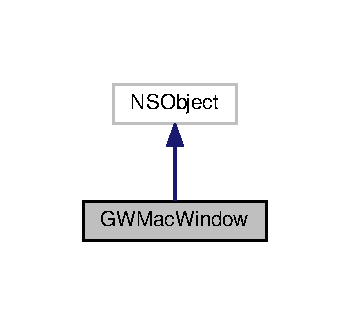
\includegraphics[width=168pt]{interfaceGWMacWindow__inherit__graph}
\end{center}
\end{figure}


Collaboration diagram for G\+W\+Mac\+Window\+:
\nopagebreak
\begin{figure}[H]
\begin{center}
\leavevmode
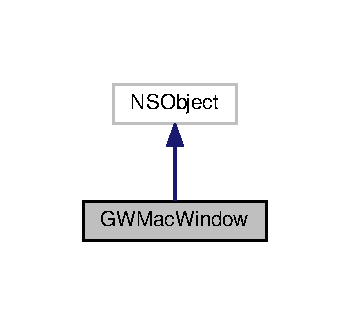
\includegraphics[width=168pt]{interfaceGWMacWindow__coll__graph}
\end{center}
\end{figure}


The documentation for this class was generated from the following file\+:\begin{DoxyCompactItemize}
\item 
Source/\+G\+\_\+\+System/G\+Window.\+mm\end{DoxyCompactItemize}

\hypertarget{interfaceGWResponder}{}\section{G\+W\+Responder Class Reference}
\label{interfaceGWResponder}\index{G\+W\+Responder@{G\+W\+Responder}}


Inheritance diagram for G\+W\+Responder\+:
\nopagebreak
\begin{figure}[H]
\begin{center}
\leavevmode
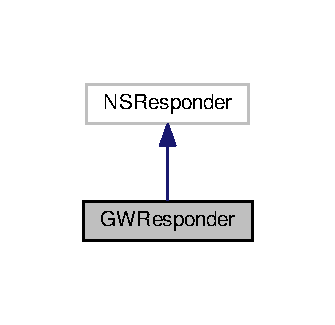
\includegraphics[width=161pt]{interfaceGWResponder__inherit__graph}
\end{center}
\end{figure}


Collaboration diagram for G\+W\+Responder\+:
\nopagebreak
\begin{figure}[H]
\begin{center}
\leavevmode
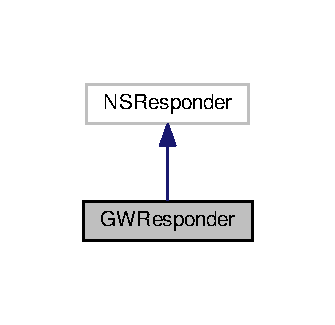
\includegraphics[width=161pt]{interfaceGWResponder__coll__graph}
\end{center}
\end{figure}
\subsection*{Instance Methods}
\begin{DoxyCompactItemize}
\item 
(bool) -\/ {\bfseries accept\+First\+Responder}\hypertarget{interfaceGWResponder_a71e98851ff4959a96d58f848ad2b882b}{}\label{interfaceGWResponder_a71e98851ff4959a96d58f848ad2b882b}

\item 
(bool) -\/ {\bfseries accepts\+First\+Mouse\+:}\hypertarget{interfaceGWResponder_a1360d3ea8830a6fc6bc3e5227d6990b0}{}\label{interfaceGWResponder_a1360d3ea8830a6fc6bc3e5227d6990b0}

\end{DoxyCompactItemize}


The documentation for this class was generated from the following file\+:\begin{DoxyCompactItemize}
\item 
Source/\+G\+\_\+\+System/G\+Window.\+mm\end{DoxyCompactItemize}

\hypertarget{structCatch_1_1IContext}{}\section{Catch\+:\+:I\+Context Struct Reference}
\label{structCatch_1_1IContext}\index{Catch\+::\+I\+Context@{Catch\+::\+I\+Context}}


Inheritance diagram for Catch\+:\+:I\+Context\+:
\nopagebreak
\begin{figure}[H]
\begin{center}
\leavevmode
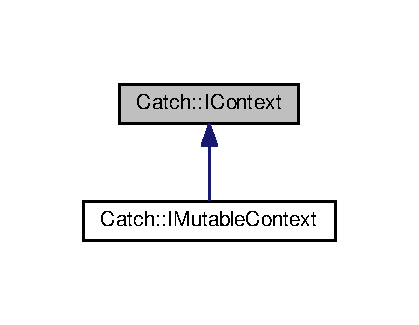
\includegraphics[width=201pt]{structCatch_1_1IContext__inherit__graph}
\end{center}
\end{figure}
\subsection*{Public Member Functions}
\begin{DoxyCompactItemize}
\item 
virtual \hyperlink{structCatch_1_1IResultCapture}{I\+Result\+Capture} $\ast$ {\bfseries get\+Result\+Capture} ()=0\hypertarget{structCatch_1_1IContext_a684e4ae71d1fdf3060c352ecde1d122f}{}\label{structCatch_1_1IContext_a684e4ae71d1fdf3060c352ecde1d122f}

\item 
virtual \hyperlink{structCatch_1_1IRunner}{I\+Runner} $\ast$ {\bfseries get\+Runner} ()=0\hypertarget{structCatch_1_1IContext_af088415dde18d039ed5a2f95b02767c6}{}\label{structCatch_1_1IContext_af088415dde18d039ed5a2f95b02767c6}

\item 
virtual size\+\_\+t {\bfseries get\+Generator\+Index} (std\+::string const \&file\+Info, size\+\_\+t total\+Size)=0\hypertarget{structCatch_1_1IContext_a43e07088db43299ba129fbe6d3106e95}{}\label{structCatch_1_1IContext_a43e07088db43299ba129fbe6d3106e95}

\item 
virtual bool {\bfseries advance\+Generators\+For\+Current\+Test} ()=0\hypertarget{structCatch_1_1IContext_a806f7c4ed24d51adae90418e661b24b7}{}\label{structCatch_1_1IContext_a806f7c4ed24d51adae90418e661b24b7}

\item 
virtual \hyperlink{classCatch_1_1Ptr}{Ptr}$<$ I\+Config const  $>$ {\bfseries get\+Config} () const =0\hypertarget{structCatch_1_1IContext_aee81c415899262e096ad8d6f686fa365}{}\label{structCatch_1_1IContext_aee81c415899262e096ad8d6f686fa365}

\end{DoxyCompactItemize}


The documentation for this struct was generated from the following file\+:\begin{DoxyCompactItemize}
\item 
Unit Tests/C\+A\+T\+C\+H.\+hpp\end{DoxyCompactItemize}

\hypertarget{structCatch_1_1IExceptionTranslator}{}\section{Catch\+:\+:I\+Exception\+Translator Struct Reference}
\label{structCatch_1_1IExceptionTranslator}\index{Catch\+::\+I\+Exception\+Translator@{Catch\+::\+I\+Exception\+Translator}}
\subsection*{Public Member Functions}
\begin{DoxyCompactItemize}
\item 
virtual std\+::string {\bfseries translate} (Exception\+Translators\+::const\+\_\+iterator it, Exception\+Translators\+::const\+\_\+iterator it\+End) const =0\hypertarget{structCatch_1_1IExceptionTranslator_a2a554b96ed5ed411e7c796b6b42837a5}{}\label{structCatch_1_1IExceptionTranslator_a2a554b96ed5ed411e7c796b6b42837a5}

\end{DoxyCompactItemize}


The documentation for this struct was generated from the following file\+:\begin{DoxyCompactItemize}
\item 
Unit Tests/C\+A\+T\+C\+H.\+hpp\end{DoxyCompactItemize}

\hypertarget{structCatch_1_1IExceptionTranslatorRegistry}{}\section{Catch\+:\+:I\+Exception\+Translator\+Registry Struct Reference}
\label{structCatch_1_1IExceptionTranslatorRegistry}\index{Catch\+::\+I\+Exception\+Translator\+Registry@{Catch\+::\+I\+Exception\+Translator\+Registry}}
\subsection*{Public Member Functions}
\begin{DoxyCompactItemize}
\item 
virtual std\+::string {\bfseries translate\+Active\+Exception} () const =0\hypertarget{structCatch_1_1IExceptionTranslatorRegistry_af76ae8c331a17f2a94c9720bc0d686bb}{}\label{structCatch_1_1IExceptionTranslatorRegistry_af76ae8c331a17f2a94c9720bc0d686bb}

\end{DoxyCompactItemize}


The documentation for this struct was generated from the following file\+:\begin{DoxyCompactItemize}
\item 
Unit Tests/C\+A\+T\+C\+H.\+hpp\end{DoxyCompactItemize}

\hypertarget{structCatch_1_1IGenerator}{}\section{Catch\+:\+:I\+Generator$<$ T $>$ Struct Template Reference}
\label{structCatch_1_1IGenerator}\index{Catch\+::\+I\+Generator$<$ T $>$@{Catch\+::\+I\+Generator$<$ T $>$}}


Inheritance diagram for Catch\+:\+:I\+Generator$<$ T $>$\+:
\nopagebreak
\begin{figure}[H]
\begin{center}
\leavevmode
\includegraphics[width=350pt]{structCatch_1_1IGenerator__inherit__graph}
\end{center}
\end{figure}
\subsection*{Public Member Functions}
\begin{DoxyCompactItemize}
\item 
virtual T {\bfseries get\+Value} (std\+::size\+\_\+t index) const =0\hypertarget{structCatch_1_1IGenerator_ad69e937cb66dba3ed9429c42abf4fce3}{}\label{structCatch_1_1IGenerator_ad69e937cb66dba3ed9429c42abf4fce3}

\item 
virtual std\+::size\+\_\+t {\bfseries size} () const =0\hypertarget{structCatch_1_1IGenerator_a2e317253b03e838b6065ce69719a198e}{}\label{structCatch_1_1IGenerator_a2e317253b03e838b6065ce69719a198e}

\end{DoxyCompactItemize}


The documentation for this struct was generated from the following file\+:\begin{DoxyCompactItemize}
\item 
Unit Tests/C\+A\+T\+C\+H.\+hpp\end{DoxyCompactItemize}

\hypertarget{structCatch_1_1IGeneratorInfo}{}\section{Catch\+:\+:I\+Generator\+Info Struct Reference}
\label{structCatch_1_1IGeneratorInfo}\index{Catch\+::\+I\+Generator\+Info@{Catch\+::\+I\+Generator\+Info}}
\subsection*{Public Member Functions}
\begin{DoxyCompactItemize}
\item 
virtual bool {\bfseries move\+Next} ()=0\hypertarget{structCatch_1_1IGeneratorInfo_a2b86711ca7009903edfe27ed62b515ef}{}\label{structCatch_1_1IGeneratorInfo_a2b86711ca7009903edfe27ed62b515ef}

\item 
virtual std\+::size\+\_\+t {\bfseries get\+Current\+Index} () const =0\hypertarget{structCatch_1_1IGeneratorInfo_a6a0dca712d31f6849fd9447b1344673a}{}\label{structCatch_1_1IGeneratorInfo_a6a0dca712d31f6849fd9447b1344673a}

\end{DoxyCompactItemize}


The documentation for this struct was generated from the following file\+:\begin{DoxyCompactItemize}
\item 
Unit Tests/C\+A\+T\+C\+H.\+hpp\end{DoxyCompactItemize}

\hypertarget{structCatch_1_1IGeneratorsForTest}{}\section{Catch\+:\+:I\+Generators\+For\+Test Struct Reference}
\label{structCatch_1_1IGeneratorsForTest}\index{Catch\+::\+I\+Generators\+For\+Test@{Catch\+::\+I\+Generators\+For\+Test}}
\subsection*{Public Member Functions}
\begin{DoxyCompactItemize}
\item 
virtual \hyperlink{structCatch_1_1IGeneratorInfo}{I\+Generator\+Info} \& {\bfseries get\+Generator\+Info} (std\+::string const \&file\+Info, std\+::size\+\_\+t size)=0\hypertarget{structCatch_1_1IGeneratorsForTest_a180d84e858840188e4c3788e47eefdb0}{}\label{structCatch_1_1IGeneratorsForTest_a180d84e858840188e4c3788e47eefdb0}

\item 
virtual bool {\bfseries move\+Next} ()=0\hypertarget{structCatch_1_1IGeneratorsForTest_adab31832d529fc584fd63164e0a1c8ad}{}\label{structCatch_1_1IGeneratorsForTest_adab31832d529fc584fd63164e0a1c8ad}

\end{DoxyCompactItemize}


The documentation for this struct was generated from the following file\+:\begin{DoxyCompactItemize}
\item 
Unit Tests/C\+A\+T\+C\+H.\+hpp\end{DoxyCompactItemize}

\hypertarget{structCatch_1_1IMutableContext}{}\section{Catch\+:\+:I\+Mutable\+Context Struct Reference}
\label{structCatch_1_1IMutableContext}\index{Catch\+::\+I\+Mutable\+Context@{Catch\+::\+I\+Mutable\+Context}}


Inheritance diagram for Catch\+:\+:I\+Mutable\+Context\+:
\nopagebreak
\begin{figure}[H]
\begin{center}
\leavevmode
\includegraphics[width=201pt]{structCatch_1_1IMutableContext__inherit__graph}
\end{center}
\end{figure}


Collaboration diagram for Catch\+:\+:I\+Mutable\+Context\+:
\nopagebreak
\begin{figure}[H]
\begin{center}
\leavevmode
\includegraphics[width=201pt]{structCatch_1_1IMutableContext__coll__graph}
\end{center}
\end{figure}
\subsection*{Public Member Functions}
\begin{DoxyCompactItemize}
\item 
virtual void {\bfseries set\+Result\+Capture} (\hyperlink{structCatch_1_1IResultCapture}{I\+Result\+Capture} $\ast$result\+Capture)=0\hypertarget{structCatch_1_1IMutableContext_a4a80afd0525b7def21bee8d9b48f2d39}{}\label{structCatch_1_1IMutableContext_a4a80afd0525b7def21bee8d9b48f2d39}

\item 
virtual void {\bfseries set\+Runner} (\hyperlink{structCatch_1_1IRunner}{I\+Runner} $\ast$runner)=0\hypertarget{structCatch_1_1IMutableContext_af2e53b1dea4527a2587cff266a730f6e}{}\label{structCatch_1_1IMutableContext_af2e53b1dea4527a2587cff266a730f6e}

\item 
virtual void {\bfseries set\+Config} (\hyperlink{classCatch_1_1Ptr}{Ptr}$<$ I\+Config const  $>$ const \&config)=0\hypertarget{structCatch_1_1IMutableContext_a04ae4f4219a481a7bf658d9fd445bc1d}{}\label{structCatch_1_1IMutableContext_a04ae4f4219a481a7bf658d9fd445bc1d}

\end{DoxyCompactItemize}


The documentation for this struct was generated from the following file\+:\begin{DoxyCompactItemize}
\item 
Unit Tests/C\+A\+T\+C\+H.\+hpp\end{DoxyCompactItemize}

\hypertarget{structCatch_1_1IMutableRegistryHub}{}\section{Catch\+:\+:I\+Mutable\+Registry\+Hub Struct Reference}
\label{structCatch_1_1IMutableRegistryHub}\index{Catch\+::\+I\+Mutable\+Registry\+Hub@{Catch\+::\+I\+Mutable\+Registry\+Hub}}
\subsection*{Public Member Functions}
\begin{DoxyCompactItemize}
\item 
virtual void {\bfseries register\+Reporter} (std\+::string const \&name, \hyperlink{classCatch_1_1Ptr}{Ptr}$<$ I\+Reporter\+Factory $>$ const \&factory)=0\hypertarget{structCatch_1_1IMutableRegistryHub_aab72d0aa1fa14627f1a6a4c893ae0a12}{}\label{structCatch_1_1IMutableRegistryHub_aab72d0aa1fa14627f1a6a4c893ae0a12}

\item 
virtual void {\bfseries register\+Listener} (\hyperlink{classCatch_1_1Ptr}{Ptr}$<$ I\+Reporter\+Factory $>$ const \&factory)=0\hypertarget{structCatch_1_1IMutableRegistryHub_ae06fcb90ba3f2b389d450cd81e229276}{}\label{structCatch_1_1IMutableRegistryHub_ae06fcb90ba3f2b389d450cd81e229276}

\item 
virtual void {\bfseries register\+Test} (\hyperlink{classCatch_1_1TestCase}{Test\+Case} const \&test\+Info)=0\hypertarget{structCatch_1_1IMutableRegistryHub_a11b85c6744d88c9f83fe16ad4a8dd451}{}\label{structCatch_1_1IMutableRegistryHub_a11b85c6744d88c9f83fe16ad4a8dd451}

\item 
virtual void {\bfseries register\+Translator} (const \hyperlink{structCatch_1_1IExceptionTranslator}{I\+Exception\+Translator} $\ast$translator)=0\hypertarget{structCatch_1_1IMutableRegistryHub_ae6825365102693cf7707db022a2c2b49}{}\label{structCatch_1_1IMutableRegistryHub_ae6825365102693cf7707db022a2c2b49}

\end{DoxyCompactItemize}


The documentation for this struct was generated from the following file\+:\begin{DoxyCompactItemize}
\item 
Unit Tests/C\+A\+T\+C\+H.\+hpp\end{DoxyCompactItemize}

\hypertarget{classInput}{}\section{Input Class Reference}
\label{classInput}\index{Input@{Input}}


Inheritance diagram for Input\+:
\nopagebreak
\begin{figure}[H]
\begin{center}
\leavevmode
\includegraphics[width=230pt]{classInput__inherit__graph}
\end{center}
\end{figure}


Collaboration diagram for Input\+:
\nopagebreak
\begin{figure}[H]
\begin{center}
\leavevmode
\includegraphics[width=230pt]{classInput__coll__graph}
\end{center}
\end{figure}
\subsection*{Public Member Functions}
\begin{DoxyCompactItemize}
\item 
void {\bfseries Input\+Thread} ()\hypertarget{classInput_a373c67d7fd7e2b81a0f498afb201b124}{}\label{classInput_a373c67d7fd7e2b81a0f498afb201b124}

\item 
\hyperlink{namespaceGW_a67a839e3df7ea8a5c5686613a7a3de21}{G\+Return} {\bfseries Initialize\+Windows} (void $\ast$\+\_\+data)\hypertarget{classInput_a180c021bb7e2e2a77325027f1e79d7fe}{}\label{classInput_a180c021bb7e2e2a77325027f1e79d7fe}

\item 
\hyperlink{namespaceGW_a67a839e3df7ea8a5c5686613a7a3de21}{G\+Return} \hyperlink{classInput_a1d195bdfcab3c160f99b1010face1e61}{Initialize\+Linux} (void $\ast$\+\_\+data)
\item 
\hyperlink{namespaceGW_a67a839e3df7ea8a5c5686613a7a3de21}{G\+Return} {\bfseries Initialize\+Mac} (void $\ast$\+\_\+data)\hypertarget{classInput_ad83dda6b9dd9388be971ff580451cfb9}{}\label{classInput_ad83dda6b9dd9388be971ff580451cfb9}

\item 
float \hyperlink{classInput_a7e468df0f31131f3fbcbc6de87d01ec2}{Get\+State} (int \+\_\+key\+Code, \hyperlink{namespaceGW_a67a839e3df7ea8a5c5686613a7a3de21}{G\+Return} $\ast$\+\_\+error\+Code)
\begin{DoxyCompactList}\small\item\em Get the current state of any key. \end{DoxyCompactList}\item 
\hyperlink{namespaceGW_a67a839e3df7ea8a5c5686613a7a3de21}{G\+Return} \hyperlink{classInput_a82d54ae7aa3ecacebe42480eb0aff985}{Get\+Mouse\+Delta} (float \&\+\_\+x, float \&\+\_\+y)
\begin{DoxyCompactList}\small\item\em Get the change in mouse position. \end{DoxyCompactList}\item 
\hyperlink{namespaceGW_a67a839e3df7ea8a5c5686613a7a3de21}{G\+Return} \hyperlink{classInput_a93d7ab591a1d1e8d619318834c75207a}{Get\+Mouse\+Position} (float \&\+\_\+x, float \&\+\_\+y)
\begin{DoxyCompactList}\small\item\em Get the most recent mouse position. \end{DoxyCompactList}\item 
unsigned int \hyperlink{classInput_a8f9b65ea323da8c25a5e70eb6746d4ab}{Get\+Key\+Mask} ()
\begin{DoxyCompactList}\small\item\em Get the key mask. \end{DoxyCompactList}\item 
\hyperlink{namespaceGW_a67a839e3df7ea8a5c5686613a7a3de21}{G\+Return} \hyperlink{classInput_a2fd6659ae76357836c4c9b3e7070ffb0}{Get\+Count} (unsigned int \&\+\_\+out\+Count)
\begin{DoxyCompactList}\small\item\em Return the total number of active references to this object. \end{DoxyCompactList}\item 
\hyperlink{namespaceGW_a67a839e3df7ea8a5c5686613a7a3de21}{G\+Return} \hyperlink{classInput_a3c2103023cbb1fa583f910539bb6cce3}{Increment\+Count} ()
\begin{DoxyCompactList}\small\item\em Increase the total number of active references to this object. \end{DoxyCompactList}\item 
\hyperlink{namespaceGW_a67a839e3df7ea8a5c5686613a7a3de21}{G\+Return} \hyperlink{classInput_a5c44b3dc2be21c1bad5f32a43a7b7a55}{Decrement\+Count} ()
\begin{DoxyCompactList}\small\item\em Decrease the total number of active references to this object. \end{DoxyCompactList}\item 
\hyperlink{namespaceGW_a67a839e3df7ea8a5c5686613a7a3de21}{G\+Return} \hyperlink{classInput_a29f3c56e9fec9f9073c1e18f120a69cd}{Request\+Interface} (const \hyperlink{structGW_1_1GUUIID}{G\+U\+U\+I\+ID} \&\+\_\+interface\+ID, void $\ast$$\ast$\+\_\+output\+Interface)
\begin{DoxyCompactList}\small\item\em Requests an interface that may or may not be supported by this object. \end{DoxyCompactList}\end{DoxyCompactItemize}


\subsection{Member Function Documentation}
\index{Input@{Input}!Decrement\+Count@{Decrement\+Count}}
\index{Decrement\+Count@{Decrement\+Count}!Input@{Input}}
\subsubsection[{\texorpdfstring{Decrement\+Count()}{DecrementCount()}}]{\setlength{\rightskip}{0pt plus 5cm}{\bf G\+Return} Input\+::\+Decrement\+Count (
\begin{DoxyParamCaption}
{}
\end{DoxyParamCaption}
)\hspace{0.3cm}{\ttfamily [virtual]}}\hypertarget{classInput_a5c44b3dc2be21c1bad5f32a43a7b7a55}{}\label{classInput_a5c44b3dc2be21c1bad5f32a43a7b7a55}


Decrease the total number of active references to this object. 

Once the internal count reaches zero this object will be deallocated and your pointer will become invalid.


\begin{DoxyRetVals}{Return values}
{\em S\+U\+C\+C\+E\+SS} & Successfully decremented the internal reference count. \\
\hline
{\em F\+A\+I\+L\+U\+RE} & Decrementing of internal reference count would underflow the value. \\
\hline
\end{DoxyRetVals}


Implements \hyperlink{classGW_1_1CORE_1_1GInterface_a19a368c77ad0aa7f49b5a4f772f173ba}{G\+W\+::\+C\+O\+R\+E\+::\+G\+Interface}.

\index{Input@{Input}!Get\+Count@{Get\+Count}}
\index{Get\+Count@{Get\+Count}!Input@{Input}}
\subsubsection[{\texorpdfstring{Get\+Count(unsigned int \&\+\_\+out\+Count)}{GetCount(unsigned int &_outCount)}}]{\setlength{\rightskip}{0pt plus 5cm}{\bf G\+Return} Input\+::\+Get\+Count (
\begin{DoxyParamCaption}
\item[{unsigned int \&}]{\+\_\+out\+Count}
\end{DoxyParamCaption}
)\hspace{0.3cm}{\ttfamily [virtual]}}\hypertarget{classInput_a2fd6659ae76357836c4c9b3e7070ffb0}{}\label{classInput_a2fd6659ae76357836c4c9b3e7070ffb0}


Return the total number of active references to this object. 


\begin{DoxyParams}[1]{Parameters}
\mbox{\tt out}  & {\em \+\_\+out\+Count} & The total number of active references of this object.\\
\hline
\end{DoxyParams}

\begin{DoxyRetVals}{Return values}
{\em S\+U\+C\+C\+E\+SS} & Successfully ran. \\
\hline
{\em F\+A\+I\+L\+U\+RE} & Either class does not exist or the internal reference count is corrupt. \\
\hline
\end{DoxyRetVals}


Implements \hyperlink{classGW_1_1CORE_1_1GInterface_aacf5834174a7024f8a3c361122ee9e76}{G\+W\+::\+C\+O\+R\+E\+::\+G\+Interface}.

\index{Input@{Input}!Get\+Key\+Mask@{Get\+Key\+Mask}}
\index{Get\+Key\+Mask@{Get\+Key\+Mask}!Input@{Input}}
\subsubsection[{\texorpdfstring{Get\+Key\+Mask()}{GetKeyMask()}}]{\setlength{\rightskip}{0pt plus 5cm}unsigned int Input\+::\+Get\+Key\+Mask (
\begin{DoxyParamCaption}
{}
\end{DoxyParamCaption}
)\hspace{0.3cm}{\ttfamily [virtual]}}\hypertarget{classInput_a8f9b65ea323da8c25a5e70eb6746d4ab}{}\label{classInput_a8f9b65ea323da8c25a5e70eb6746d4ab}


Get the key mask. 

The key mask lets the input object know which of the functions below are active by manipulating individual bits of an unsigned int.


\begin{DoxyRetVals}{Return values}
{\em G\+\_\+\+M\+A\+SK} & (\+\_\+\+S\+H\+I\+FT, \+\_\+\+C\+O\+N\+T\+R\+OL, \+\_\+\+C\+A\+P\+S\+\_\+\+L\+O\+CK, \+\_\+\+N\+U\+M\+\_\+\+L\+O\+CK, \+\_\+\+S\+C\+R\+O\+L\+L\+\_\+\+L\+O\+CK). \\
\hline
\end{DoxyRetVals}


Implements \hyperlink{classGW_1_1SYSTEM_1_1GInput_a071a399bc9c400f0cd333958d911c8c2}{G\+W\+::\+S\+Y\+S\+T\+E\+M\+::\+G\+Input}.

\index{Input@{Input}!Get\+Mouse\+Delta@{Get\+Mouse\+Delta}}
\index{Get\+Mouse\+Delta@{Get\+Mouse\+Delta}!Input@{Input}}
\subsubsection[{\texorpdfstring{Get\+Mouse\+Delta(float \&\+\_\+x, float \&\+\_\+y)}{GetMouseDelta(float &_x, float &_y)}}]{\setlength{\rightskip}{0pt plus 5cm}{\bf G\+Return} Input\+::\+Get\+Mouse\+Delta (
\begin{DoxyParamCaption}
\item[{float \&}]{x, }
\item[{float \&}]{y}
\end{DoxyParamCaption}
)\hspace{0.3cm}{\ttfamily [virtual]}}\hypertarget{classInput_a82d54ae7aa3ecacebe42480eb0aff985}{}\label{classInput_a82d54ae7aa3ecacebe42480eb0aff985}


Get the change in mouse position. 


\begin{DoxyParams}[1]{Parameters}
\mbox{\tt out}  & {\em x} & a reference to a float to store the mouse delta position x. \\
\hline
\mbox{\tt out}  & {\em y} & a reference to a float to store the mouse delta position y.\\
\hline
\end{DoxyParams}

\begin{DoxyRetVals}{Return values}
{\em S\+U\+C\+C\+E\+SS} & no problems found. Values stored in x and y. \\
\hline
\end{DoxyRetVals}


Implements \hyperlink{classGW_1_1SYSTEM_1_1GInput_a2c968f0195241813dea705fb9a02a8b5}{G\+W\+::\+S\+Y\+S\+T\+E\+M\+::\+G\+Input}.

\index{Input@{Input}!Get\+Mouse\+Position@{Get\+Mouse\+Position}}
\index{Get\+Mouse\+Position@{Get\+Mouse\+Position}!Input@{Input}}
\subsubsection[{\texorpdfstring{Get\+Mouse\+Position(float \&\+\_\+x, float \&\+\_\+y)}{GetMousePosition(float &_x, float &_y)}}]{\setlength{\rightskip}{0pt plus 5cm}{\bf G\+Return} Input\+::\+Get\+Mouse\+Position (
\begin{DoxyParamCaption}
\item[{float \&}]{x, }
\item[{float \&}]{y}
\end{DoxyParamCaption}
)\hspace{0.3cm}{\ttfamily [virtual]}}\hypertarget{classInput_a93d7ab591a1d1e8d619318834c75207a}{}\label{classInput_a93d7ab591a1d1e8d619318834c75207a}


Get the most recent mouse position. 


\begin{DoxyParams}[1]{Parameters}
\mbox{\tt out}  & {\em x} & a reference to a float to store the mouse position x. \\
\hline
\mbox{\tt out}  & {\em y} & a reference to a float to store the mouse position y.\\
\hline
\end{DoxyParams}

\begin{DoxyRetVals}{Return values}
{\em S\+U\+C\+C\+E\+SS} & no problems found. Values stored in x and y. \\
\hline
\end{DoxyRetVals}


Implements \hyperlink{classGW_1_1SYSTEM_1_1GInput_af0d0f1a00a2ebd04d5d697d1468c3c00}{G\+W\+::\+S\+Y\+S\+T\+E\+M\+::\+G\+Input}.

\index{Input@{Input}!Get\+State@{Get\+State}}
\index{Get\+State@{Get\+State}!Input@{Input}}
\subsubsection[{\texorpdfstring{Get\+State(int \+\_\+key\+Code, G\+Return $\ast$\+\_\+error\+Code)}{GetState(int _keyCode, GReturn *_errorCode)}}]{\setlength{\rightskip}{0pt plus 5cm}float Input\+::\+Get\+State (
\begin{DoxyParamCaption}
\item[{int}]{\+\_\+key\+Code, }
\item[{{\bf G\+Return} $\ast$}]{error\+Code}
\end{DoxyParamCaption}
)\hspace{0.3cm}{\ttfamily [virtual]}}\hypertarget{classInput_a7e468df0f31131f3fbcbc6de87d01ec2}{}\label{classInput_a7e468df0f31131f3fbcbc6de87d01ec2}


Get the current state of any key. 

Use keycodes in G\+Key\+Defines as input to this function to check the state of a particular key or button.


\begin{DoxyParams}[1]{Parameters}
\mbox{\tt in}  & {\em \+\_\+key\+Code} & The key code of the key to check. \\
\hline
\mbox{\tt out}  & {\em error\+Code} & If function fails this will hold the error\+Code.\\
\hline
\end{DoxyParams}

\begin{DoxyRetVals}{Return values}
{\em 0} & The Key is not pressed. \\
\hline
{\em 1} & The Key is pressed. \\
\hline
\end{DoxyRetVals}


Implements \hyperlink{classGW_1_1SYSTEM_1_1GInput_a7a3e93a3730d05cfeb92fc1dd93ad07a}{G\+W\+::\+S\+Y\+S\+T\+E\+M\+::\+G\+Input}.

\index{Input@{Input}!Increment\+Count@{Increment\+Count}}
\index{Increment\+Count@{Increment\+Count}!Input@{Input}}
\subsubsection[{\texorpdfstring{Increment\+Count()}{IncrementCount()}}]{\setlength{\rightskip}{0pt plus 5cm}{\bf G\+Return} Input\+::\+Increment\+Count (
\begin{DoxyParamCaption}
{}
\end{DoxyParamCaption}
)\hspace{0.3cm}{\ttfamily [virtual]}}\hypertarget{classInput_a3c2103023cbb1fa583f910539bb6cce3}{}\label{classInput_a3c2103023cbb1fa583f910539bb6cce3}


Increase the total number of active references to this object. 

End users should only call this operation if they are familiar with reference counting behavior.


\begin{DoxyRetVals}{Return values}
{\em S\+U\+C\+C\+E\+SS} & Successfully incremented the internal reference count. \\
\hline
{\em F\+A\+I\+L\+U\+RE} & Incrementation of internal reference count would overflow the value. \\
\hline
\end{DoxyRetVals}


Implements \hyperlink{classGW_1_1CORE_1_1GInterface_a2d710f20bb78e544e8309b5b75c21260}{G\+W\+::\+C\+O\+R\+E\+::\+G\+Interface}.

\index{Input@{Input}!Initialize\+Linux@{Initialize\+Linux}}
\index{Initialize\+Linux@{Initialize\+Linux}!Input@{Input}}
\subsubsection[{\texorpdfstring{Initialize\+Linux(void $\ast$\+\_\+data)}{InitializeLinux(void *_data)}}]{\setlength{\rightskip}{0pt plus 5cm}{\bf G\+Return} Input\+::\+Initialize\+Linux (
\begin{DoxyParamCaption}
\item[{void $\ast$}]{\+\_\+data}
\end{DoxyParamCaption}
)}\hypertarget{classInput_a1d195bdfcab3c160f99b1010face1e61}{}\label{classInput_a1d195bdfcab3c160f99b1010face1e61}
X\+Auto\+Repeat\+Off(\+\_\+display); \index{Input@{Input}!Request\+Interface@{Request\+Interface}}
\index{Request\+Interface@{Request\+Interface}!Input@{Input}}
\subsubsection[{\texorpdfstring{Request\+Interface(const G\+U\+U\+I\+I\+D \&\+\_\+interface\+I\+D, void $\ast$$\ast$\+\_\+output\+Interface)}{RequestInterface(const GUUIID &_interfaceID, void **_outputInterface)}}]{\setlength{\rightskip}{0pt plus 5cm}{\bf G\+Return} Input\+::\+Request\+Interface (
\begin{DoxyParamCaption}
\item[{const {\bf G\+U\+U\+I\+ID} \&}]{\+\_\+interface\+ID, }
\item[{void $\ast$$\ast$}]{\+\_\+output\+Interface}
\end{DoxyParamCaption}
)\hspace{0.3cm}{\ttfamily [virtual]}}\hypertarget{classInput_a29f3c56e9fec9f9073c1e18f120a69cd}{}\label{classInput_a29f3c56e9fec9f9073c1e18f120a69cd}


Requests an interface that may or may not be supported by this object. 

Can be used by the end-\/user to query for a new interface using the unique ID of the interface they want and implement an interface update.


\begin{DoxyParams}[1]{Parameters}
\mbox{\tt in}  & {\em \+\_\+interface\+ID} & The G\+U\+U\+I\+ID of the interface you are requesting. \\
\hline
\mbox{\tt out}  & {\em \+\_\+output\+Interface} & Where the interface will be stored if function is successful.\\
\hline
\end{DoxyParams}

\begin{DoxyRetVals}{Return values}
{\em S\+U\+C\+C\+E\+SS} & The interface is supported and function succeded. \\
\hline
{\em I\+N\+T\+E\+R\+F\+A\+C\+E\+\_\+\+U\+N\+S\+U\+P\+P\+O\+R\+T\+ED} & The requested interface is not supported. \\
\hline
\end{DoxyRetVals}


Implements \hyperlink{classGW_1_1CORE_1_1GInterface_ad6c8324970172784964f484686d4fdad}{G\+W\+::\+C\+O\+R\+E\+::\+G\+Interface}.



The documentation for this class was generated from the following file\+:\begin{DoxyCompactItemize}
\item 
Source/\+G\+\_\+\+System/G\+Input.\+cpp\end{DoxyCompactItemize}

\hypertarget{structCatch_1_1IRegistryHub}{}\section{Catch\+:\+:I\+Registry\+Hub Struct Reference}
\label{structCatch_1_1IRegistryHub}\index{Catch\+::\+I\+Registry\+Hub@{Catch\+::\+I\+Registry\+Hub}}
\subsection*{Public Member Functions}
\begin{DoxyCompactItemize}
\item 
virtual I\+Reporter\+Registry const \& {\bfseries get\+Reporter\+Registry} () const =0\hypertarget{structCatch_1_1IRegistryHub_a55534563f7ecf7e20ec1e37285ebe54d}{}\label{structCatch_1_1IRegistryHub_a55534563f7ecf7e20ec1e37285ebe54d}

\item 
virtual \hyperlink{structCatch_1_1ITestCaseRegistry}{I\+Test\+Case\+Registry} const \& {\bfseries get\+Test\+Case\+Registry} () const =0\hypertarget{structCatch_1_1IRegistryHub_af4f6255f0c0f8f1f179fa9d7d4843076}{}\label{structCatch_1_1IRegistryHub_af4f6255f0c0f8f1f179fa9d7d4843076}

\item 
virtual \hyperlink{structCatch_1_1IExceptionTranslatorRegistry}{I\+Exception\+Translator\+Registry} \& {\bfseries get\+Exception\+Translator\+Registry} ()=0\hypertarget{structCatch_1_1IRegistryHub_a3606988da110c016c5af3ae63454eb78}{}\label{structCatch_1_1IRegistryHub_a3606988da110c016c5af3ae63454eb78}

\end{DoxyCompactItemize}


The documentation for this struct was generated from the following file\+:\begin{DoxyCompactItemize}
\item 
Unit Tests/C\+A\+T\+C\+H.\+hpp\end{DoxyCompactItemize}

\hypertarget{structCatch_1_1IResultCapture}{}\section{Catch\+:\+:I\+Result\+Capture Struct Reference}
\label{structCatch_1_1IResultCapture}\index{Catch\+::\+I\+Result\+Capture@{Catch\+::\+I\+Result\+Capture}}
\subsection*{Public Member Functions}
\begin{DoxyCompactItemize}
\item 
virtual void {\bfseries assertion\+Ended} (\hyperlink{classCatch_1_1AssertionResult}{Assertion\+Result} const \&result)=0\hypertarget{structCatch_1_1IResultCapture_ae45e08bccc5fb434656d4f2e44742223}{}\label{structCatch_1_1IResultCapture_ae45e08bccc5fb434656d4f2e44742223}

\item 
virtual bool {\bfseries section\+Started} (\hyperlink{structCatch_1_1SectionInfo}{Section\+Info} const \&section\+Info, \hyperlink{structCatch_1_1Counts}{Counts} \&assertions)=0\hypertarget{structCatch_1_1IResultCapture_a5b76ed52badcb64cf374202e12b81a03}{}\label{structCatch_1_1IResultCapture_a5b76ed52badcb64cf374202e12b81a03}

\item 
virtual void {\bfseries section\+Ended} (\hyperlink{structCatch_1_1SectionEndInfo}{Section\+End\+Info} const \&end\+Info)=0\hypertarget{structCatch_1_1IResultCapture_a4e152bc43dc0933684e31fa67a58195d}{}\label{structCatch_1_1IResultCapture_a4e152bc43dc0933684e31fa67a58195d}

\item 
virtual void {\bfseries section\+Ended\+Early} (\hyperlink{structCatch_1_1SectionEndInfo}{Section\+End\+Info} const \&end\+Info)=0\hypertarget{structCatch_1_1IResultCapture_afcc71eef8ca821ae132cced4a2be6988}{}\label{structCatch_1_1IResultCapture_afcc71eef8ca821ae132cced4a2be6988}

\item 
virtual void {\bfseries push\+Scoped\+Message} (\hyperlink{structCatch_1_1MessageInfo}{Message\+Info} const \&message)=0\hypertarget{structCatch_1_1IResultCapture_a91d154c1e087e383dcde5aad95cb6a05}{}\label{structCatch_1_1IResultCapture_a91d154c1e087e383dcde5aad95cb6a05}

\item 
virtual void {\bfseries pop\+Scoped\+Message} (\hyperlink{structCatch_1_1MessageInfo}{Message\+Info} const \&message)=0\hypertarget{structCatch_1_1IResultCapture_a42bcb13276706bf8c3ce081ce16d37fd}{}\label{structCatch_1_1IResultCapture_a42bcb13276706bf8c3ce081ce16d37fd}

\item 
virtual std\+::string {\bfseries get\+Current\+Test\+Name} () const =0\hypertarget{structCatch_1_1IResultCapture_aea1617f4a84cc648246aa3ed6918b5bf}{}\label{structCatch_1_1IResultCapture_aea1617f4a84cc648246aa3ed6918b5bf}

\item 
virtual const \hyperlink{classCatch_1_1AssertionResult}{Assertion\+Result} $\ast$ {\bfseries get\+Last\+Result} () const =0\hypertarget{structCatch_1_1IResultCapture_ab18872c89fab97405a56e9c6a4919736}{}\label{structCatch_1_1IResultCapture_ab18872c89fab97405a56e9c6a4919736}

\item 
virtual void {\bfseries handle\+Fatal\+Error\+Condition} (std\+::string const \&message)=0\hypertarget{structCatch_1_1IResultCapture_a7d995222301e6605f26549726b30c3ee}{}\label{structCatch_1_1IResultCapture_a7d995222301e6605f26549726b30c3ee}

\end{DoxyCompactItemize}


The documentation for this struct was generated from the following file\+:\begin{DoxyCompactItemize}
\item 
Unit Tests/C\+A\+T\+C\+H.\+hpp\end{DoxyCompactItemize}

\hypertarget{structCatch_1_1IRunner}{}\section{Catch\+:\+:I\+Runner Struct Reference}
\label{structCatch_1_1IRunner}\index{Catch\+::\+I\+Runner@{Catch\+::\+I\+Runner}}
\subsection*{Public Member Functions}
\begin{DoxyCompactItemize}
\item 
virtual bool {\bfseries aborting} () const =0\hypertarget{structCatch_1_1IRunner_a03713202dd2e041e30b8030088ab0116}{}\label{structCatch_1_1IRunner_a03713202dd2e041e30b8030088ab0116}

\end{DoxyCompactItemize}


The documentation for this struct was generated from the following file\+:\begin{DoxyCompactItemize}
\item 
Unit Tests/C\+A\+T\+C\+H.\+hpp\end{DoxyCompactItemize}

\hypertarget{structCatch_1_1IShared}{}\section{Catch\+:\+:I\+Shared Struct Reference}
\label{structCatch_1_1IShared}\index{Catch\+::\+I\+Shared@{Catch\+::\+I\+Shared}}


Inheritance diagram for Catch\+:\+:I\+Shared\+:
\nopagebreak
\begin{figure}[H]
\begin{center}
\leavevmode
\includegraphics[width=350pt]{structCatch_1_1IShared__inherit__graph}
\end{center}
\end{figure}


Collaboration diagram for Catch\+:\+:I\+Shared\+:
\nopagebreak
\begin{figure}[H]
\begin{center}
\leavevmode
\includegraphics[width=188pt]{structCatch_1_1IShared__coll__graph}
\end{center}
\end{figure}
\subsection*{Public Member Functions}
\begin{DoxyCompactItemize}
\item 
virtual void {\bfseries add\+Ref} () const =0\hypertarget{structCatch_1_1IShared_ae383df68557cdaf0910b411af04d9e33}{}\label{structCatch_1_1IShared_ae383df68557cdaf0910b411af04d9e33}

\item 
virtual void {\bfseries release} () const =0\hypertarget{structCatch_1_1IShared_a002f52624728a763956fb6f230cb2f57}{}\label{structCatch_1_1IShared_a002f52624728a763956fb6f230cb2f57}

\end{DoxyCompactItemize}


The documentation for this struct was generated from the following file\+:\begin{DoxyCompactItemize}
\item 
Unit Tests/C\+A\+T\+C\+H.\+hpp\end{DoxyCompactItemize}

\hypertarget{structCatch_1_1Detail_1_1IsStreamInsertable}{}\section{Catch\+:\+:Detail\+:\+:Is\+Stream\+Insertable$<$ T $>$ Struct Template Reference}
\label{structCatch_1_1Detail_1_1IsStreamInsertable}\index{Catch\+::\+Detail\+::\+Is\+Stream\+Insertable$<$ T $>$@{Catch\+::\+Detail\+::\+Is\+Stream\+Insertable$<$ T $>$}}
\subsection*{Public Types}
\begin{DoxyCompactItemize}
\item 
enum \{ {\bfseries value} = sizeof(test\+Streamable(s $<$$<$ t)) == sizeof(True\+Type)
 \}\hypertarget{structCatch_1_1Detail_1_1IsStreamInsertable_acb41cf4cda793be95dbda63bbea8a721}{}\label{structCatch_1_1Detail_1_1IsStreamInsertable_acb41cf4cda793be95dbda63bbea8a721}

\end{DoxyCompactItemize}
\subsection*{Static Public Attributes}
\begin{DoxyCompactItemize}
\item 
static std\+::ostream \& {\bfseries s}\hypertarget{structCatch_1_1Detail_1_1IsStreamInsertable_abe3d3c8e5d85665747faafffc9a96b00}{}\label{structCatch_1_1Detail_1_1IsStreamInsertable_abe3d3c8e5d85665747faafffc9a96b00}

\item 
static T const \& {\bfseries t}\hypertarget{structCatch_1_1Detail_1_1IsStreamInsertable_a7d2a3da978b6736667a7b2f6d51f507f}{}\label{structCatch_1_1Detail_1_1IsStreamInsertable_a7d2a3da978b6736667a7b2f6d51f507f}

\end{DoxyCompactItemize}


The documentation for this struct was generated from the following file\+:\begin{DoxyCompactItemize}
\item 
Unit Tests/C\+A\+T\+C\+H.\+hpp\end{DoxyCompactItemize}

\hypertarget{structCatch_1_1ITagAliasRegistry}{}\section{Catch\+:\+:I\+Tag\+Alias\+Registry Struct Reference}
\label{structCatch_1_1ITagAliasRegistry}\index{Catch\+::\+I\+Tag\+Alias\+Registry@{Catch\+::\+I\+Tag\+Alias\+Registry}}
\subsection*{Public Member Functions}
\begin{DoxyCompactItemize}
\item 
virtual \hyperlink{classCatch_1_1Option}{Option}$<$ \hyperlink{structCatch_1_1TagAlias}{Tag\+Alias} $>$ {\bfseries find} (std\+::string const \&alias) const =0\hypertarget{structCatch_1_1ITagAliasRegistry_a7d2fba4d39cfcc62c2695fcde4f989c3}{}\label{structCatch_1_1ITagAliasRegistry_a7d2fba4d39cfcc62c2695fcde4f989c3}

\item 
virtual std\+::string {\bfseries expand\+Aliases} (std\+::string const \&unexpanded\+Test\+Spec) const =0\hypertarget{structCatch_1_1ITagAliasRegistry_ae729a7532faf7466db1a157ce0395170}{}\label{structCatch_1_1ITagAliasRegistry_ae729a7532faf7466db1a157ce0395170}

\end{DoxyCompactItemize}
\subsection*{Static Public Member Functions}
\begin{DoxyCompactItemize}
\item 
static \hyperlink{structCatch_1_1ITagAliasRegistry}{I\+Tag\+Alias\+Registry} const \& {\bfseries get} ()\hypertarget{structCatch_1_1ITagAliasRegistry_aa9d0f008f49473389c7abf6071f137a7}{}\label{structCatch_1_1ITagAliasRegistry_aa9d0f008f49473389c7abf6071f137a7}

\end{DoxyCompactItemize}


The documentation for this struct was generated from the following file\+:\begin{DoxyCompactItemize}
\item 
Unit Tests/C\+A\+T\+C\+H.\+hpp\end{DoxyCompactItemize}

\hypertarget{structCatch_1_1ITestCase}{}\section{Catch\+:\+:I\+Test\+Case Struct Reference}
\label{structCatch_1_1ITestCase}\index{Catch\+::\+I\+Test\+Case@{Catch\+::\+I\+Test\+Case}}


Inheritance diagram for Catch\+:\+:I\+Test\+Case\+:
\nopagebreak
\begin{figure}[H]
\begin{center}
\leavevmode
\includegraphics[width=229pt]{structCatch_1_1ITestCase__inherit__graph}
\end{center}
\end{figure}


Collaboration diagram for Catch\+:\+:I\+Test\+Case\+:
\nopagebreak
\begin{figure}[H]
\begin{center}
\leavevmode
\includegraphics[width=188pt]{structCatch_1_1ITestCase__coll__graph}
\end{center}
\end{figure}
\subsection*{Public Member Functions}
\begin{DoxyCompactItemize}
\item 
virtual void {\bfseries invoke} () const =0\hypertarget{structCatch_1_1ITestCase_a678825e62e7c17297621cfeb65588c34}{}\label{structCatch_1_1ITestCase_a678825e62e7c17297621cfeb65588c34}

\end{DoxyCompactItemize}


The documentation for this struct was generated from the following file\+:\begin{DoxyCompactItemize}
\item 
Unit Tests/C\+A\+T\+C\+H.\+hpp\end{DoxyCompactItemize}

\hypertarget{structCatch_1_1ITestCaseRegistry}{}\section{Catch\+:\+:I\+Test\+Case\+Registry Struct Reference}
\label{structCatch_1_1ITestCaseRegistry}\index{Catch\+::\+I\+Test\+Case\+Registry@{Catch\+::\+I\+Test\+Case\+Registry}}
\subsection*{Public Member Functions}
\begin{DoxyCompactItemize}
\item 
virtual std\+::vector$<$ \hyperlink{classCatch_1_1TestCase}{Test\+Case} $>$ const \& {\bfseries get\+All\+Tests} () const =0\hypertarget{structCatch_1_1ITestCaseRegistry_ad6e4d4a621655123f73ae98cfeda063d}{}\label{structCatch_1_1ITestCaseRegistry_ad6e4d4a621655123f73ae98cfeda063d}

\item 
virtual std\+::vector$<$ \hyperlink{classCatch_1_1TestCase}{Test\+Case} $>$ const \& {\bfseries get\+All\+Tests\+Sorted} (I\+Config const \&config) const =0\hypertarget{structCatch_1_1ITestCaseRegistry_a33e46639d0319d35497c05bb5d02be5a}{}\label{structCatch_1_1ITestCaseRegistry_a33e46639d0319d35497c05bb5d02be5a}

\end{DoxyCompactItemize}


The documentation for this struct was generated from the following file\+:\begin{DoxyCompactItemize}
\item 
Unit Tests/C\+A\+T\+C\+H.\+hpp\end{DoxyCompactItemize}

\hypertarget{structGW_1_1SYSTEM_1_1LINUX__WINDOW}{}\section{GW\+::S\+Y\+S\+T\+EM\+::L\+I\+N\+U\+X\+\_\+\+W\+I\+N\+D\+OW Struct Reference}
\label{structGW_1_1SYSTEM_1_1LINUX__WINDOW}\index{GW::SYSTEM::LINUX\_WINDOW@{GW::SYSTEM::LINUX\_WINDOW}}


The structure used to pass into Input libraries on Linux.  




{\ttfamily \#include $<$G\+Key\+Defines.\+h$>$}

\subsection*{Public Attributes}
\begin{DoxyCompactItemize}
\item 
\mbox{\Hypertarget{structGW_1_1SYSTEM_1_1LINUX__WINDOW_a9d4ffe1d048716af5f2d1fe3595b6b99}\label{structGW_1_1SYSTEM_1_1LINUX__WINDOW_a9d4ffe1d048716af5f2d1fe3595b6b99}} 
void $\ast$ {\bfseries window}
\item 
\mbox{\Hypertarget{structGW_1_1SYSTEM_1_1LINUX__WINDOW_ae68b93065e8ebd9de010f42ccf688ac5}\label{structGW_1_1SYSTEM_1_1LINUX__WINDOW_ae68b93065e8ebd9de010f42ccf688ac5}} 
void $\ast$ {\bfseries display}
\end{DoxyCompactItemize}


\subsection{Detailed Description}
The structure used to pass into Input libraries on Linux. 

The documentation for this struct was generated from the following file\+:\begin{DoxyCompactItemize}
\item 
Interface/\+G\+\_\+\+System/G\+Key\+Defines.\+h\end{DoxyCompactItemize}

\hypertarget{classLogFile}{}\section{Log\+File Class Reference}
\label{classLogFile}\index{Log\+File@{Log\+File}}


Inheritance diagram for Log\+File\+:
\nopagebreak
\begin{figure}[H]
\begin{center}
\leavevmode
\includegraphics[width=224pt]{classLogFile__inherit__graph}
\end{center}
\end{figure}


Collaboration diagram for Log\+File\+:
\nopagebreak
\begin{figure}[H]
\begin{center}
\leavevmode
\includegraphics[width=224pt]{classLogFile__coll__graph}
\end{center}
\end{figure}
\subsection*{Public Member Functions}
\begin{DoxyCompactItemize}
\item 
\hyperlink{namespaceGW_a67a839e3df7ea8a5c5686613a7a3de21}{G\+W\+::\+G\+Return} {\bfseries Init} (const char $\ast$const \+\_\+file\+Name)\hypertarget{classLogFile_a3347793c16a8888a130b10404c9e5ece}{}\label{classLogFile_a3347793c16a8888a130b10404c9e5ece}

\item 
\hyperlink{namespaceGW_a67a839e3df7ea8a5c5686613a7a3de21}{G\+W\+::\+G\+Return} {\bfseries Init} (\hyperlink{classGW_1_1SYSTEM_1_1GFile}{G\+W\+::\+S\+Y\+S\+T\+E\+M\+::\+G\+File} $\ast$\+\_\+file)\hypertarget{classLogFile_afd658429cf77f9bbf48e2ebb72b9c6e2}{}\label{classLogFile_afd658429cf77f9bbf48e2ebb72b9c6e2}

\item 
\hyperlink{namespaceGW_a67a839e3df7ea8a5c5686613a7a3de21}{G\+W\+::\+G\+Return} \hyperlink{classLogFile_a6848c12fad15f2c835e5215234f75c5a}{Log} (const char $\ast$const \+\_\+log) override
\begin{DoxyCompactList}\small\item\em Logs a null terminated string. \end{DoxyCompactList}\item 
\hyperlink{namespaceGW_a67a839e3df7ea8a5c5686613a7a3de21}{G\+W\+::\+G\+Return} \hyperlink{classLogFile_a5e5f24ccd4c6f925dd8bc1ced512b530}{Log\+Catergorized} (const char $\ast$const \+\_\+category, const char $\ast$const \+\_\+log) override
\begin{DoxyCompactList}\small\item\em Logs a null terminated string with a category. \end{DoxyCompactList}\item 
void \hyperlink{classLogFile_a250bcfaccded12f7da9a06b6f6336fa5}{Enable\+Verbose\+Logging} (bool \+\_\+value) override
\begin{DoxyCompactList}\small\item\em Turns verbose logging on or off. \end{DoxyCompactList}\item 
void \hyperlink{classLogFile_a903b31947e1c100309dcc5b20548262c}{Enable\+Console\+Logging} (bool \+\_\+value) override
\begin{DoxyCompactList}\small\item\em Turns console logging on or off. \end{DoxyCompactList}\item 
\hyperlink{namespaceGW_a67a839e3df7ea8a5c5686613a7a3de21}{G\+W\+::\+G\+Return} \hyperlink{classLogFile_a47ffb41f72625b1c7865ac2cd58dea18}{Flush} () override
\begin{DoxyCompactList}\small\item\em Forces a log dump to file. \end{DoxyCompactList}\item 
\hyperlink{namespaceGW_a67a839e3df7ea8a5c5686613a7a3de21}{G\+W\+::\+G\+Return} \hyperlink{classLogFile_ab2abbdb01e2b904f112e5e7b20c59a81}{Get\+Count} (unsigned int \&\+\_\+out\+Count) override
\begin{DoxyCompactList}\small\item\em Return the total number of active references to this object. \end{DoxyCompactList}\item 
\hyperlink{namespaceGW_a67a839e3df7ea8a5c5686613a7a3de21}{G\+W\+::\+G\+Return} \hyperlink{classLogFile_aff5871b4f2434b6ca722b89581416da0}{Increment\+Count} () override
\begin{DoxyCompactList}\small\item\em Increase the total number of active references to this object. \end{DoxyCompactList}\item 
\hyperlink{namespaceGW_a67a839e3df7ea8a5c5686613a7a3de21}{G\+W\+::\+G\+Return} \hyperlink{classLogFile_a555ef35fcdce23ebad05f7dcabaf0757}{Decrement\+Count} () override
\begin{DoxyCompactList}\small\item\em Decrease the total number of active references to this object. \end{DoxyCompactList}\item 
\hyperlink{namespaceGW_a67a839e3df7ea8a5c5686613a7a3de21}{G\+W\+::\+G\+Return} \hyperlink{classLogFile_a8b8e63b9c62846b1b9e0cf8b79429ba5}{Request\+Interface} (const \hyperlink{structGW_1_1GUUIID}{G\+W\+::\+G\+U\+U\+I\+ID} \&\+\_\+interface\+ID, void $\ast$$\ast$\+\_\+output\+Interface) override
\begin{DoxyCompactList}\small\item\em Requests an interface that may or may not be supported by this object. \end{DoxyCompactList}\end{DoxyCompactItemize}


\subsection{Member Function Documentation}
\index{Log\+File@{Log\+File}!Decrement\+Count@{Decrement\+Count}}
\index{Decrement\+Count@{Decrement\+Count}!Log\+File@{Log\+File}}
\subsubsection[{\texorpdfstring{Decrement\+Count() override}{DecrementCount() override}}]{\setlength{\rightskip}{0pt plus 5cm}{\bf G\+W\+::\+G\+Return} Log\+File\+::\+Decrement\+Count (
\begin{DoxyParamCaption}
{}
\end{DoxyParamCaption}
)\hspace{0.3cm}{\ttfamily [override]}, {\ttfamily [virtual]}}\hypertarget{classLogFile_a555ef35fcdce23ebad05f7dcabaf0757}{}\label{classLogFile_a555ef35fcdce23ebad05f7dcabaf0757}


Decrease the total number of active references to this object. 

Once the internal count reaches zero this object will be deallocated and your pointer will become invalid.


\begin{DoxyRetVals}{Return values}
{\em S\+U\+C\+C\+E\+SS} & Successfully decremented the internal reference count. \\
\hline
{\em F\+A\+I\+L\+U\+RE} & Decrementing of internal reference count would underflow the value. \\
\hline
\end{DoxyRetVals}


Implements \hyperlink{classGW_1_1CORE_1_1GInterface_a19a368c77ad0aa7f49b5a4f772f173ba}{G\+W\+::\+C\+O\+R\+E\+::\+G\+Interface}.

\index{Log\+File@{Log\+File}!Enable\+Console\+Logging@{Enable\+Console\+Logging}}
\index{Enable\+Console\+Logging@{Enable\+Console\+Logging}!Log\+File@{Log\+File}}
\subsubsection[{\texorpdfstring{Enable\+Console\+Logging(bool \+\_\+value) override}{EnableConsoleLogging(bool _value) override}}]{\setlength{\rightskip}{0pt plus 5cm}void Log\+File\+::\+Enable\+Console\+Logging (
\begin{DoxyParamCaption}
\item[{bool}]{\+\_\+value}
\end{DoxyParamCaption}
)\hspace{0.3cm}{\ttfamily [override]}, {\ttfamily [virtual]}}\hypertarget{classLogFile_a903b31947e1c100309dcc5b20548262c}{}\label{classLogFile_a903b31947e1c100309dcc5b20548262c}


Turns console logging on or off. 

Use this function to ensure or prevent the additional console logging.


\begin{DoxyParams}[1]{Parameters}
\mbox{\tt in}  & {\em \+\_\+value} & true to turn on or false to turn off. \\
\hline
\end{DoxyParams}


Implements \hyperlink{classGW_1_1SYSTEM_1_1GLog_abceb9fdf502b11f2fe72de5edd8f187d}{G\+W\+::\+S\+Y\+S\+T\+E\+M\+::\+G\+Log}.

\index{Log\+File@{Log\+File}!Enable\+Verbose\+Logging@{Enable\+Verbose\+Logging}}
\index{Enable\+Verbose\+Logging@{Enable\+Verbose\+Logging}!Log\+File@{Log\+File}}
\subsubsection[{\texorpdfstring{Enable\+Verbose\+Logging(bool \+\_\+value) override}{EnableVerboseLogging(bool _value) override}}]{\setlength{\rightskip}{0pt plus 5cm}void Log\+File\+::\+Enable\+Verbose\+Logging (
\begin{DoxyParamCaption}
\item[{bool}]{\+\_\+value}
\end{DoxyParamCaption}
)\hspace{0.3cm}{\ttfamily [override]}, {\ttfamily [virtual]}}\hypertarget{classLogFile_a250bcfaccded12f7da9a06b6f6336fa5}{}\label{classLogFile_a250bcfaccded12f7da9a06b6f6336fa5}


Turns verbose logging on or off. 

Use this function to ensure or prevent the addition of date, time, and thread\+ID to your log messages.


\begin{DoxyParams}[1]{Parameters}
\mbox{\tt in}  & {\em \+\_\+value} & true to turn on or false to turn off. \\
\hline
\end{DoxyParams}


Implements \hyperlink{classGW_1_1SYSTEM_1_1GLog_a4323c96541a34fb0344828a1c20ec254}{G\+W\+::\+S\+Y\+S\+T\+E\+M\+::\+G\+Log}.

\index{Log\+File@{Log\+File}!Flush@{Flush}}
\index{Flush@{Flush}!Log\+File@{Log\+File}}
\subsubsection[{\texorpdfstring{Flush() override}{Flush() override}}]{\setlength{\rightskip}{0pt plus 5cm}{\bf G\+W\+::\+G\+Return} Log\+File\+::\+Flush (
\begin{DoxyParamCaption}
{}
\end{DoxyParamCaption}
)\hspace{0.3cm}{\ttfamily [override]}, {\ttfamily [virtual]}}\hypertarget{classLogFile_a47ffb41f72625b1c7865ac2cd58dea18}{}\label{classLogFile_a47ffb41f72625b1c7865ac2cd58dea18}


Forces a log dump to file. 

This will force a log dump to the file and clear the log queue.


\begin{DoxyRetVals}{Return values}
{\em S\+U\+C\+C\+E\+SS} & Successfully dumped the logs. \\
\hline
{\em F\+A\+I\+L\+U\+RE} & Most likely a file corruption or a file is not open. \\
\hline
\end{DoxyRetVals}


Implements \hyperlink{classGW_1_1SYSTEM_1_1GLog_a07147c15ecb17caa1c83974b3c54f7d4}{G\+W\+::\+S\+Y\+S\+T\+E\+M\+::\+G\+Log}.

\index{Log\+File@{Log\+File}!Get\+Count@{Get\+Count}}
\index{Get\+Count@{Get\+Count}!Log\+File@{Log\+File}}
\subsubsection[{\texorpdfstring{Get\+Count(unsigned int \&\+\_\+out\+Count) override}{GetCount(unsigned int &_outCount) override}}]{\setlength{\rightskip}{0pt plus 5cm}{\bf G\+W\+::\+G\+Return} Log\+File\+::\+Get\+Count (
\begin{DoxyParamCaption}
\item[{unsigned int \&}]{\+\_\+out\+Count}
\end{DoxyParamCaption}
)\hspace{0.3cm}{\ttfamily [override]}, {\ttfamily [virtual]}}\hypertarget{classLogFile_ab2abbdb01e2b904f112e5e7b20c59a81}{}\label{classLogFile_ab2abbdb01e2b904f112e5e7b20c59a81}


Return the total number of active references to this object. 


\begin{DoxyParams}[1]{Parameters}
\mbox{\tt out}  & {\em \+\_\+out\+Count} & The total number of active references of this object.\\
\hline
\end{DoxyParams}

\begin{DoxyRetVals}{Return values}
{\em S\+U\+C\+C\+E\+SS} & Successfully ran. \\
\hline
{\em F\+A\+I\+L\+U\+RE} & Either class does not exist or the internal reference count is corrupt. \\
\hline
\end{DoxyRetVals}


Implements \hyperlink{classGW_1_1CORE_1_1GInterface_aacf5834174a7024f8a3c361122ee9e76}{G\+W\+::\+C\+O\+R\+E\+::\+G\+Interface}.

\index{Log\+File@{Log\+File}!Increment\+Count@{Increment\+Count}}
\index{Increment\+Count@{Increment\+Count}!Log\+File@{Log\+File}}
\subsubsection[{\texorpdfstring{Increment\+Count() override}{IncrementCount() override}}]{\setlength{\rightskip}{0pt plus 5cm}{\bf G\+W\+::\+G\+Return} Log\+File\+::\+Increment\+Count (
\begin{DoxyParamCaption}
{}
\end{DoxyParamCaption}
)\hspace{0.3cm}{\ttfamily [override]}, {\ttfamily [virtual]}}\hypertarget{classLogFile_aff5871b4f2434b6ca722b89581416da0}{}\label{classLogFile_aff5871b4f2434b6ca722b89581416da0}


Increase the total number of active references to this object. 

End users should only call this operation if they are familiar with reference counting behavior.


\begin{DoxyRetVals}{Return values}
{\em S\+U\+C\+C\+E\+SS} & Successfully incremented the internal reference count. \\
\hline
{\em F\+A\+I\+L\+U\+RE} & Incrementation of internal reference count would overflow the value. \\
\hline
\end{DoxyRetVals}


Implements \hyperlink{classGW_1_1CORE_1_1GInterface_a2d710f20bb78e544e8309b5b75c21260}{G\+W\+::\+C\+O\+R\+E\+::\+G\+Interface}.

\index{Log\+File@{Log\+File}!Log@{Log}}
\index{Log@{Log}!Log\+File@{Log\+File}}
\subsubsection[{\texorpdfstring{Log(const char $\ast$const \+\_\+log) override}{Log(const char *const _log) override}}]{\setlength{\rightskip}{0pt plus 5cm}{\bf G\+W\+::\+G\+Return} Log\+File\+::\+Log (
\begin{DoxyParamCaption}
\item[{const char $\ast$const}]{\+\_\+log}
\end{DoxyParamCaption}
)\hspace{0.3cm}{\ttfamily [override]}, {\ttfamily [virtual]}}\hypertarget{classLogFile_a6848c12fad15f2c835e5215234f75c5a}{}\label{classLogFile_a6848c12fad15f2c835e5215234f75c5a}


Logs a null terminated string. 

Date, Time, and thread ID will be appended to the front of the message unless specified otherwise (See Enable\+Verbose\+Logging). A new line character will be appended to the end of the string so your log messages do not require a new line. The string is logged to the internal G\+File object.


\begin{DoxyParams}[1]{Parameters}
\mbox{\tt in}  & {\em \+\_\+log} & The message to log out.\\
\hline
\end{DoxyParams}

\begin{DoxyRetVals}{Return values}
{\em S\+U\+C\+C\+E\+SS} & Successfully queued the message to the log. \\
\hline
{\em F\+A\+I\+L\+U\+RE} & The queue has reached maximum size (call flush). \\
\hline
{\em I\+N\+V\+A\+L\+I\+D\+\_\+\+A\+R\+G\+U\+M\+E\+NT} & A nullptr was passed in. \\
\hline
\end{DoxyRetVals}


Implements \hyperlink{classGW_1_1SYSTEM_1_1GLog_a9e21e702d012065fe799b4c49f7ac670}{G\+W\+::\+S\+Y\+S\+T\+E\+M\+::\+G\+Log}.

\index{Log\+File@{Log\+File}!Log\+Catergorized@{Log\+Catergorized}}
\index{Log\+Catergorized@{Log\+Catergorized}!Log\+File@{Log\+File}}
\subsubsection[{\texorpdfstring{Log\+Catergorized(const char $\ast$const \+\_\+category, const char $\ast$const \+\_\+log) override}{LogCatergorized(const char *const _category, const char *const _log) override}}]{\setlength{\rightskip}{0pt plus 5cm}{\bf G\+W\+::\+G\+Return} Log\+File\+::\+Log\+Catergorized (
\begin{DoxyParamCaption}
\item[{const char $\ast$const}]{\+\_\+category, }
\item[{const char $\ast$const}]{\+\_\+log}
\end{DoxyParamCaption}
)\hspace{0.3cm}{\ttfamily [override]}, {\ttfamily [virtual]}}\hypertarget{classLogFile_a5e5f24ccd4c6f925dd8bc1ced512b530}{}\label{classLogFile_a5e5f24ccd4c6f925dd8bc1ced512b530}


Logs a null terminated string with a category. 

Date, Time, and thread ID will be appended to the front of the message unless specified otherwise (See Enable\+Verbose\+Logging). A new line character will be appended to the end of the string so your log messages do not require a new line. The string is logged to the internal G\+File object.


\begin{DoxyParams}[1]{Parameters}
\mbox{\tt in}  & {\em \+\_\+category} & The category the log belongs in. ie. E\+R\+R\+OR, W\+A\+R\+N\+I\+NG, I\+N\+FO, etc. \\
\hline
\mbox{\tt in}  & {\em \+\_\+log} & The message to log out.\\
\hline
\end{DoxyParams}

\begin{DoxyRetVals}{Return values}
{\em S\+U\+C\+C\+E\+SS} & Successfully queued the message to the log. \\
\hline
{\em F\+A\+I\+L\+U\+RE} & The queue has reached maximum size (call flush). \\
\hline
{\em I\+N\+V\+A\+L\+I\+D\+\_\+\+A\+R\+G\+U\+M\+E\+NT} & Either \+\_\+category or \+\_\+log are nullptr. \\
\hline
\end{DoxyRetVals}


Implements \hyperlink{classGW_1_1SYSTEM_1_1GLog_a5d10397fa6aeeebaf8430df6029ec3c5}{G\+W\+::\+S\+Y\+S\+T\+E\+M\+::\+G\+Log}.

\index{Log\+File@{Log\+File}!Request\+Interface@{Request\+Interface}}
\index{Request\+Interface@{Request\+Interface}!Log\+File@{Log\+File}}
\subsubsection[{\texorpdfstring{Request\+Interface(const G\+W\+::\+G\+U\+U\+I\+I\+D \&\+\_\+interface\+I\+D, void $\ast$$\ast$\+\_\+output\+Interface) override}{RequestInterface(const GW::GUUIID &_interfaceID, void **_outputInterface) override}}]{\setlength{\rightskip}{0pt plus 5cm}{\bf G\+W\+::\+G\+Return} Log\+File\+::\+Request\+Interface (
\begin{DoxyParamCaption}
\item[{const {\bf G\+W\+::\+G\+U\+U\+I\+ID} \&}]{\+\_\+interface\+ID, }
\item[{void $\ast$$\ast$}]{\+\_\+output\+Interface}
\end{DoxyParamCaption}
)\hspace{0.3cm}{\ttfamily [override]}, {\ttfamily [virtual]}}\hypertarget{classLogFile_a8b8e63b9c62846b1b9e0cf8b79429ba5}{}\label{classLogFile_a8b8e63b9c62846b1b9e0cf8b79429ba5}


Requests an interface that may or may not be supported by this object. 

Can be used by the end-\/user to query for a new interface using the unique ID of the interface they want and implement an interface update.


\begin{DoxyParams}[1]{Parameters}
\mbox{\tt in}  & {\em \+\_\+interface\+ID} & The G\+U\+U\+I\+ID of the interface you are requesting. \\
\hline
\mbox{\tt out}  & {\em \+\_\+output\+Interface} & Where the interface will be stored if function is successful.\\
\hline
\end{DoxyParams}

\begin{DoxyRetVals}{Return values}
{\em S\+U\+C\+C\+E\+SS} & The interface is supported and function succeded. \\
\hline
{\em I\+N\+T\+E\+R\+F\+A\+C\+E\+\_\+\+U\+N\+S\+U\+P\+P\+O\+R\+T\+ED} & The requested interface is not supported. \\
\hline
\end{DoxyRetVals}


Implements \hyperlink{classGW_1_1CORE_1_1GInterface_ad6c8324970172784964f484686d4fdad}{G\+W\+::\+C\+O\+R\+E\+::\+G\+Interface}.



The documentation for this class was generated from the following file\+:\begin{DoxyCompactItemize}
\item 
Source/\+G\+\_\+\+System/G\+Log.\+cpp\end{DoxyCompactItemize}

\hypertarget{structCatch_1_1Matchers_1_1Impl_1_1Matcher}{}\section{Catch\+:\+:Matchers\+:\+:Impl\+:\+:Matcher$<$ ExpressionT $>$ Struct Template Reference}
\label{structCatch_1_1Matchers_1_1Impl_1_1Matcher}\index{Catch\+::\+Matchers\+::\+Impl\+::\+Matcher$<$ Expression\+T $>$@{Catch\+::\+Matchers\+::\+Impl\+::\+Matcher$<$ Expression\+T $>$}}


Inheritance diagram for Catch\+:\+:Matchers\+:\+:Impl\+:\+:Matcher$<$ ExpressionT $>$\+:
\nopagebreak
\begin{figure}[H]
\begin{center}
\leavevmode
\includegraphics[width=350pt]{structCatch_1_1Matchers_1_1Impl_1_1Matcher__inherit__graph}
\end{center}
\end{figure}


Collaboration diagram for Catch\+:\+:Matchers\+:\+:Impl\+:\+:Matcher$<$ ExpressionT $>$\+:
\nopagebreak
\begin{figure}[H]
\begin{center}
\leavevmode
\includegraphics[width=211pt]{structCatch_1_1Matchers_1_1Impl_1_1Matcher__coll__graph}
\end{center}
\end{figure}
\subsection*{Public Types}
\begin{DoxyCompactItemize}
\item 
typedef ExpressionT {\bfseries Expression\+Type}\hypertarget{structCatch_1_1Matchers_1_1Impl_1_1Matcher_a7f5068cbacd1eed06cf243e63446e7e1}{}\label{structCatch_1_1Matchers_1_1Impl_1_1Matcher_a7f5068cbacd1eed06cf243e63446e7e1}

\end{DoxyCompactItemize}
\subsection*{Public Member Functions}
\begin{DoxyCompactItemize}
\item 
virtual \hyperlink{classCatch_1_1Ptr}{Ptr}$<$ \hyperlink{structCatch_1_1Matchers_1_1Impl_1_1Matcher}{Matcher} $>$ {\bfseries clone} () const =0\hypertarget{structCatch_1_1Matchers_1_1Impl_1_1Matcher_a9d31e5018fea24efa08c3cbf5aa4475d}{}\label{structCatch_1_1Matchers_1_1Impl_1_1Matcher_a9d31e5018fea24efa08c3cbf5aa4475d}

\item 
virtual bool {\bfseries match} (ExpressionT const \&expr) const =0\hypertarget{structCatch_1_1Matchers_1_1Impl_1_1Matcher_a8c1c5511ce1f3738a45e6901b558f583}{}\label{structCatch_1_1Matchers_1_1Impl_1_1Matcher_a8c1c5511ce1f3738a45e6901b558f583}

\item 
virtual std\+::string {\bfseries to\+String} () const =0\hypertarget{structCatch_1_1Matchers_1_1Impl_1_1Matcher_a091bcc37e589967d7e10fc7790d820e2}{}\label{structCatch_1_1Matchers_1_1Impl_1_1Matcher_a091bcc37e589967d7e10fc7790d820e2}

\item 
\hyperlink{classCatch_1_1Matchers_1_1Impl_1_1Generic_1_1AllOf}{Generic\+::\+All\+Of}$<$ ExpressionT $>$ {\bfseries operator\&\&} (\hyperlink{structCatch_1_1Matchers_1_1Impl_1_1Matcher}{Matcher}$<$ ExpressionT $>$ const \&other) const \hypertarget{structCatch_1_1Matchers_1_1Impl_1_1Matcher_a1d3b73f684611a6a71396caf74427287}{}\label{structCatch_1_1Matchers_1_1Impl_1_1Matcher_a1d3b73f684611a6a71396caf74427287}

\item 
\hyperlink{classCatch_1_1Matchers_1_1Impl_1_1Generic_1_1AnyOf}{Generic\+::\+Any\+Of}$<$ ExpressionT $>$ {\bfseries operator$\vert$$\vert$} (\hyperlink{structCatch_1_1Matchers_1_1Impl_1_1Matcher}{Matcher}$<$ ExpressionT $>$ const \&other) const \hypertarget{structCatch_1_1Matchers_1_1Impl_1_1Matcher_a2e163b264811ba76638469b537467f9e}{}\label{structCatch_1_1Matchers_1_1Impl_1_1Matcher_a2e163b264811ba76638469b537467f9e}

\item 
\hyperlink{classCatch_1_1Matchers_1_1Impl_1_1Generic_1_1Not}{Generic\+::\+Not}$<$ ExpressionT $>$ {\bfseries operator!} () const \hypertarget{structCatch_1_1Matchers_1_1Impl_1_1Matcher_a534857633dde84924993b674cb248c8f}{}\label{structCatch_1_1Matchers_1_1Impl_1_1Matcher_a534857633dde84924993b674cb248c8f}

\end{DoxyCompactItemize}
\subsection*{Additional Inherited Members}


The documentation for this struct was generated from the following file\+:\begin{DoxyCompactItemize}
\item 
Unit Tests/C\+A\+T\+C\+H.\+hpp\end{DoxyCompactItemize}

\hypertarget{structCatch_1_1Matchers_1_1Impl_1_1MatcherImpl}{}\section{Catch\+:\+:Matchers\+:\+:Impl\+:\+:Matcher\+Impl$<$ DerivedT, ExpressionT $>$ Struct Template Reference}
\label{structCatch_1_1Matchers_1_1Impl_1_1MatcherImpl}\index{Catch\+::\+Matchers\+::\+Impl\+::\+Matcher\+Impl$<$ Derived\+T, Expression\+T $>$@{Catch\+::\+Matchers\+::\+Impl\+::\+Matcher\+Impl$<$ Derived\+T, Expression\+T $>$}}


Inheritance diagram for Catch\+:\+:Matchers\+:\+:Impl\+:\+:Matcher\+Impl$<$ DerivedT, ExpressionT $>$\+:
\nopagebreak
\begin{figure}[H]
\begin{center}
\leavevmode
\includegraphics[width=211pt]{structCatch_1_1Matchers_1_1Impl_1_1MatcherImpl__inherit__graph}
\end{center}
\end{figure}


Collaboration diagram for Catch\+:\+:Matchers\+:\+:Impl\+:\+:Matcher\+Impl$<$ DerivedT, ExpressionT $>$\+:
\nopagebreak
\begin{figure}[H]
\begin{center}
\leavevmode
\includegraphics[width=211pt]{structCatch_1_1Matchers_1_1Impl_1_1MatcherImpl__coll__graph}
\end{center}
\end{figure}
\subsection*{Public Member Functions}
\begin{DoxyCompactItemize}
\item 
virtual \hyperlink{classCatch_1_1Ptr}{Ptr}$<$ \hyperlink{structCatch_1_1Matchers_1_1Impl_1_1Matcher}{Matcher}$<$ ExpressionT $>$ $>$ {\bfseries clone} () const \hypertarget{structCatch_1_1Matchers_1_1Impl_1_1MatcherImpl_afe2e10779f91394f80ff5c894fb1bfab}{}\label{structCatch_1_1Matchers_1_1Impl_1_1MatcherImpl_afe2e10779f91394f80ff5c894fb1bfab}

\end{DoxyCompactItemize}
\subsection*{Additional Inherited Members}


The documentation for this struct was generated from the following file\+:\begin{DoxyCompactItemize}
\item 
Unit Tests/C\+A\+T\+C\+H.\+hpp\end{DoxyCompactItemize}

\hypertarget{structCatch_1_1MessageBuilder}{}\section{Catch\+:\+:Message\+Builder Struct Reference}
\label{structCatch_1_1MessageBuilder}\index{Catch\+::\+Message\+Builder@{Catch\+::\+Message\+Builder}}


Collaboration diagram for Catch\+:\+:Message\+Builder\+:
\nopagebreak
\begin{figure}[H]
\begin{center}
\leavevmode
\includegraphics[width=288pt]{structCatch_1_1MessageBuilder__coll__graph}
\end{center}
\end{figure}
\subsection*{Public Member Functions}
\begin{DoxyCompactItemize}
\item 
{\bfseries Message\+Builder} (std\+::string const \&macro\+Name, \hyperlink{structCatch_1_1SourceLineInfo}{Source\+Line\+Info} const \&line\+Info, Result\+Was\+::\+Of\+Type type)\hypertarget{structCatch_1_1MessageBuilder_ab0c6378e722680bf58852c6ee2b6e724}{}\label{structCatch_1_1MessageBuilder_ab0c6378e722680bf58852c6ee2b6e724}

\item 
{\footnotesize template$<$typename T $>$ }\\\hyperlink{structCatch_1_1MessageBuilder}{Message\+Builder} \& {\bfseries operator$<$$<$} (T const \&value)\hypertarget{structCatch_1_1MessageBuilder_a20fa48d069b20dddcc2d3df8abb123c1}{}\label{structCatch_1_1MessageBuilder_a20fa48d069b20dddcc2d3df8abb123c1}

\end{DoxyCompactItemize}
\subsection*{Public Attributes}
\begin{DoxyCompactItemize}
\item 
\hyperlink{structCatch_1_1MessageInfo}{Message\+Info} {\bfseries m\+\_\+info}\hypertarget{structCatch_1_1MessageBuilder_a979f1c2b36d78f80ee275bfa5ba0209f}{}\label{structCatch_1_1MessageBuilder_a979f1c2b36d78f80ee275bfa5ba0209f}

\item 
std\+::ostringstream {\bfseries m\+\_\+stream}\hypertarget{structCatch_1_1MessageBuilder_a6488ab0cc4ea52affc9c0612c7c5df6b}{}\label{structCatch_1_1MessageBuilder_a6488ab0cc4ea52affc9c0612c7c5df6b}

\end{DoxyCompactItemize}


The documentation for this struct was generated from the following file\+:\begin{DoxyCompactItemize}
\item 
Unit Tests/C\+A\+T\+C\+H.\+hpp\end{DoxyCompactItemize}

\hypertarget{structCatch_1_1MessageInfo}{}\section{Catch\+:\+:Message\+Info Struct Reference}
\label{structCatch_1_1MessageInfo}\index{Catch\+::\+Message\+Info@{Catch\+::\+Message\+Info}}


Collaboration diagram for Catch\+:\+:Message\+Info\+:
\nopagebreak
\begin{figure}[H]
\begin{center}
\leavevmode
\includegraphics[width=281pt]{structCatch_1_1MessageInfo__coll__graph}
\end{center}
\end{figure}
\subsection*{Public Member Functions}
\begin{DoxyCompactItemize}
\item 
{\bfseries Message\+Info} (std\+::string const \&\+\_\+macro\+Name, \hyperlink{structCatch_1_1SourceLineInfo}{Source\+Line\+Info} const \&\+\_\+line\+Info, Result\+Was\+::\+Of\+Type \+\_\+type)\hypertarget{structCatch_1_1MessageInfo_a2e336c33ebef7af3c1bbae6a56e14f8a}{}\label{structCatch_1_1MessageInfo_a2e336c33ebef7af3c1bbae6a56e14f8a}

\item 
bool {\bfseries operator==} (\hyperlink{structCatch_1_1MessageInfo}{Message\+Info} const \&other) const \hypertarget{structCatch_1_1MessageInfo_a30fe117138e568c5a9dfdabb7de6e790}{}\label{structCatch_1_1MessageInfo_a30fe117138e568c5a9dfdabb7de6e790}

\item 
bool {\bfseries operator$<$} (\hyperlink{structCatch_1_1MessageInfo}{Message\+Info} const \&other) const \hypertarget{structCatch_1_1MessageInfo_a7a2b1ec3772cd35176e2ee25a94be16a}{}\label{structCatch_1_1MessageInfo_a7a2b1ec3772cd35176e2ee25a94be16a}

\end{DoxyCompactItemize}
\subsection*{Public Attributes}
\begin{DoxyCompactItemize}
\item 
std\+::string {\bfseries macro\+Name}\hypertarget{structCatch_1_1MessageInfo_a156ade4b3cc731f6ec7b542ae47ba8e3}{}\label{structCatch_1_1MessageInfo_a156ade4b3cc731f6ec7b542ae47ba8e3}

\item 
\hyperlink{structCatch_1_1SourceLineInfo}{Source\+Line\+Info} {\bfseries line\+Info}\hypertarget{structCatch_1_1MessageInfo_a985165328723e599696ebd8e43195cc5}{}\label{structCatch_1_1MessageInfo_a985165328723e599696ebd8e43195cc5}

\item 
Result\+Was\+::\+Of\+Type {\bfseries type}\hypertarget{structCatch_1_1MessageInfo_ae928b9117465c696e45951d9d0284e78}{}\label{structCatch_1_1MessageInfo_ae928b9117465c696e45951d9d0284e78}

\item 
std\+::string {\bfseries message}\hypertarget{structCatch_1_1MessageInfo_ab6cd06e050bf426c6577502a5c50e256}{}\label{structCatch_1_1MessageInfo_ab6cd06e050bf426c6577502a5c50e256}

\item 
unsigned int {\bfseries sequence}\hypertarget{structCatch_1_1MessageInfo_a7f4f57ea21e50160adefce7b68a781d6}{}\label{structCatch_1_1MessageInfo_a7f4f57ea21e50160adefce7b68a781d6}

\end{DoxyCompactItemize}


The documentation for this struct was generated from the following file\+:\begin{DoxyCompactItemize}
\item 
Unit Tests/C\+A\+T\+C\+H.\+hpp\end{DoxyCompactItemize}

\hypertarget{classCatch_1_1MethodTestCase}{}\section{Catch\+:\+:Method\+Test\+Case$<$ C $>$ Class Template Reference}
\label{classCatch_1_1MethodTestCase}\index{Catch\+::\+Method\+Test\+Case$<$ C $>$@{Catch\+::\+Method\+Test\+Case$<$ C $>$}}


Inheritance diagram for Catch\+:\+:Method\+Test\+Case$<$ C $>$\+:
\nopagebreak
\begin{figure}[H]
\begin{center}
\leavevmode
\includegraphics[width=229pt]{classCatch_1_1MethodTestCase__inherit__graph}
\end{center}
\end{figure}


Collaboration diagram for Catch\+:\+:Method\+Test\+Case$<$ C $>$\+:
\nopagebreak
\begin{figure}[H]
\begin{center}
\leavevmode
\includegraphics[width=229pt]{classCatch_1_1MethodTestCase__coll__graph}
\end{center}
\end{figure}
\subsection*{Public Member Functions}
\begin{DoxyCompactItemize}
\item 
{\bfseries Method\+Test\+Case} (void(C\+::$\ast$method)())\hypertarget{classCatch_1_1MethodTestCase_a7b043b85dae371358255dd9dc6582e7b}{}\label{classCatch_1_1MethodTestCase_a7b043b85dae371358255dd9dc6582e7b}

\item 
virtual void {\bfseries invoke} () const \hypertarget{classCatch_1_1MethodTestCase_a39cc4b760dd71adc3f7550bc1e7eb697}{}\label{classCatch_1_1MethodTestCase_a39cc4b760dd71adc3f7550bc1e7eb697}

\end{DoxyCompactItemize}
\subsection*{Additional Inherited Members}


The documentation for this class was generated from the following file\+:\begin{DoxyCompactItemize}
\item 
Unit Tests/C\+A\+T\+C\+H.\+hpp\end{DoxyCompactItemize}

\hypertarget{structCatch_1_1NameAndDesc}{}\section{Catch\+:\+:Name\+And\+Desc Struct Reference}
\label{structCatch_1_1NameAndDesc}\index{Catch\+::\+Name\+And\+Desc@{Catch\+::\+Name\+And\+Desc}}
\subsection*{Public Member Functions}
\begin{DoxyCompactItemize}
\item 
{\bfseries Name\+And\+Desc} (const char $\ast$\+\_\+name=\char`\"{}\char`\"{}, const char $\ast$\+\_\+description=\char`\"{}\char`\"{})\hypertarget{structCatch_1_1NameAndDesc_a189ceb9942fb5f6635140d6a09fc843a}{}\label{structCatch_1_1NameAndDesc_a189ceb9942fb5f6635140d6a09fc843a}

\end{DoxyCompactItemize}
\subsection*{Public Attributes}
\begin{DoxyCompactItemize}
\item 
const char $\ast$ {\bfseries name}\hypertarget{structCatch_1_1NameAndDesc_a374b4ed8be3cf98be20ebde5273bde51}{}\label{structCatch_1_1NameAndDesc_a374b4ed8be3cf98be20ebde5273bde51}

\item 
const char $\ast$ {\bfseries description}\hypertarget{structCatch_1_1NameAndDesc_a3463a23ff65ce494fc380452b57b7970}{}\label{structCatch_1_1NameAndDesc_a3463a23ff65ce494fc380452b57b7970}

\end{DoxyCompactItemize}


The documentation for this struct was generated from the following file\+:\begin{DoxyCompactItemize}
\item 
Unit Tests/C\+A\+T\+C\+H.\+hpp\end{DoxyCompactItemize}

\hypertarget{classCatch_1_1NonCopyable}{}\section{Catch\+:\+:Non\+Copyable Class Reference}
\label{classCatch_1_1NonCopyable}\index{Catch\+::\+Non\+Copyable@{Catch\+::\+Non\+Copyable}}


Inheritance diagram for Catch\+:\+:Non\+Copyable\+:
\nopagebreak
\begin{figure}[H]
\begin{center}
\leavevmode
\includegraphics[width=350pt]{classCatch_1_1NonCopyable__inherit__graph}
\end{center}
\end{figure}


The documentation for this class was generated from the following file\+:\begin{DoxyCompactItemize}
\item 
Unit Tests/C\+A\+T\+C\+H.\+hpp\end{DoxyCompactItemize}

\hypertarget{classCatch_1_1Matchers_1_1Impl_1_1Generic_1_1Not}{}\section{Catch\+:\+:Matchers\+:\+:Impl\+:\+:Generic\+:\+:Not$<$ ExpressionT $>$ Class Template Reference}
\label{classCatch_1_1Matchers_1_1Impl_1_1Generic_1_1Not}\index{Catch\+::\+Matchers\+::\+Impl\+::\+Generic\+::\+Not$<$ Expression\+T $>$@{Catch\+::\+Matchers\+::\+Impl\+::\+Generic\+::\+Not$<$ Expression\+T $>$}}


Inheritance diagram for Catch\+:\+:Matchers\+:\+:Impl\+:\+:Generic\+:\+:Not$<$ ExpressionT $>$\+:
\nopagebreak
\begin{figure}[H]
\begin{center}
\leavevmode
\includegraphics[width=239pt]{classCatch_1_1Matchers_1_1Impl_1_1Generic_1_1Not__inherit__graph}
\end{center}
\end{figure}


Collaboration diagram for Catch\+:\+:Matchers\+:\+:Impl\+:\+:Generic\+:\+:Not$<$ ExpressionT $>$\+:
\nopagebreak
\begin{figure}[H]
\begin{center}
\leavevmode
\includegraphics[width=239pt]{classCatch_1_1Matchers_1_1Impl_1_1Generic_1_1Not__coll__graph}
\end{center}
\end{figure}
\subsection*{Public Member Functions}
\begin{DoxyCompactItemize}
\item 
{\bfseries Not} (\hyperlink{structCatch_1_1Matchers_1_1Impl_1_1Matcher}{Matcher}$<$ ExpressionT $>$ const \&matcher)\hypertarget{classCatch_1_1Matchers_1_1Impl_1_1Generic_1_1Not_a9b99e3ce49c1a16931708b67c312f204}{}\label{classCatch_1_1Matchers_1_1Impl_1_1Generic_1_1Not_a9b99e3ce49c1a16931708b67c312f204}

\item 
{\bfseries Not} (\hyperlink{classCatch_1_1Matchers_1_1Impl_1_1Generic_1_1Not}{Not} const \&other)\hypertarget{classCatch_1_1Matchers_1_1Impl_1_1Generic_1_1Not_a46eccbbaeec259d3536aa2a29f95208f}{}\label{classCatch_1_1Matchers_1_1Impl_1_1Generic_1_1Not_a46eccbbaeec259d3536aa2a29f95208f}

\item 
virtual bool {\bfseries match} (ExpressionT const \&expr) const C\+A\+T\+C\+H\+\_\+\+O\+V\+E\+R\+R\+I\+DE\hypertarget{classCatch_1_1Matchers_1_1Impl_1_1Generic_1_1Not_a18c49fc6fb73a42d54650dafc18c7db1}{}\label{classCatch_1_1Matchers_1_1Impl_1_1Generic_1_1Not_a18c49fc6fb73a42d54650dafc18c7db1}

\item 
virtual std\+::string {\bfseries to\+String} () const C\+A\+T\+C\+H\+\_\+\+O\+V\+E\+R\+R\+I\+DE\hypertarget{classCatch_1_1Matchers_1_1Impl_1_1Generic_1_1Not_ab970a4a6e58a987451e0b0e0e60a0bff}{}\label{classCatch_1_1Matchers_1_1Impl_1_1Generic_1_1Not_ab970a4a6e58a987451e0b0e0e60a0bff}

\end{DoxyCompactItemize}
\subsection*{Additional Inherited Members}


The documentation for this class was generated from the following file\+:\begin{DoxyCompactItemize}
\item 
Unit Tests/C\+A\+T\+C\+H.\+hpp\end{DoxyCompactItemize}

\hypertarget{classCatch_1_1NotImplementedException}{}\section{Catch\+:\+:Not\+Implemented\+Exception Class Reference}
\label{classCatch_1_1NotImplementedException}\index{Catch\+::\+Not\+Implemented\+Exception@{Catch\+::\+Not\+Implemented\+Exception}}


Inheritance diagram for Catch\+:\+:Not\+Implemented\+Exception\+:
\nopagebreak
\begin{figure}[H]
\begin{center}
\leavevmode
\includegraphics[width=244pt]{classCatch_1_1NotImplementedException__inherit__graph}
\end{center}
\end{figure}


Collaboration diagram for Catch\+:\+:Not\+Implemented\+Exception\+:
\nopagebreak
\begin{figure}[H]
\begin{center}
\leavevmode
\includegraphics[width=244pt]{classCatch_1_1NotImplementedException__coll__graph}
\end{center}
\end{figure}
\subsection*{Public Member Functions}
\begin{DoxyCompactItemize}
\item 
{\bfseries Not\+Implemented\+Exception} (\hyperlink{structCatch_1_1SourceLineInfo}{Source\+Line\+Info} const \&line\+Info)\hypertarget{classCatch_1_1NotImplementedException_ab4f0a5c39d8ffb72c664e2c07e180634}{}\label{classCatch_1_1NotImplementedException_ab4f0a5c39d8ffb72c664e2c07e180634}

\item 
{\bfseries Not\+Implemented\+Exception} (\hyperlink{classCatch_1_1NotImplementedException}{Not\+Implemented\+Exception} const \&)\hypertarget{classCatch_1_1NotImplementedException_a508a7a833455da2d3c10ea1a9d45e982}{}\label{classCatch_1_1NotImplementedException_a508a7a833455da2d3c10ea1a9d45e982}

\item 
virtual const char $\ast$ {\bfseries what} () const C\+A\+T\+C\+H\+\_\+\+N\+O\+E\+X\+C\+E\+PT\hypertarget{classCatch_1_1NotImplementedException_ad4c13963f1a8feacda0cd331adda89e3}{}\label{classCatch_1_1NotImplementedException_ad4c13963f1a8feacda0cd331adda89e3}

\end{DoxyCompactItemize}


The documentation for this class was generated from the following file\+:\begin{DoxyCompactItemize}
\item 
Unit Tests/C\+A\+T\+C\+H.\+hpp\end{DoxyCompactItemize}

\hypertarget{structCatch_1_1Internal_1_1OperatorTraits}{}\section{Catch\+:\+:Internal\+:\+:Operator\+Traits$<$ Op $>$ Struct Template Reference}
\label{structCatch_1_1Internal_1_1OperatorTraits}\index{Catch\+::\+Internal\+::\+Operator\+Traits$<$ Op $>$@{Catch\+::\+Internal\+::\+Operator\+Traits$<$ Op $>$}}
\subsection*{Static Public Member Functions}
\begin{DoxyCompactItemize}
\item 
static const char $\ast$ {\bfseries get\+Name} ()\hypertarget{structCatch_1_1Internal_1_1OperatorTraits_ac6d08082ea33348d42bc4ccbd6d07671}{}\label{structCatch_1_1Internal_1_1OperatorTraits_ac6d08082ea33348d42bc4ccbd6d07671}

\end{DoxyCompactItemize}


The documentation for this struct was generated from the following file\+:\begin{DoxyCompactItemize}
\item 
Unit Tests/C\+A\+T\+C\+H.\+hpp\end{DoxyCompactItemize}

\hypertarget{structCatch_1_1Internal_1_1OperatorTraits_3_01IsEqualTo_01_4}{}\section{Catch\+:\+:Internal\+:\+:Operator\+Traits$<$ Is\+Equal\+To $>$ Struct Template Reference}
\label{structCatch_1_1Internal_1_1OperatorTraits_3_01IsEqualTo_01_4}\index{Catch\+::\+Internal\+::\+Operator\+Traits$<$ Is\+Equal\+To $>$@{Catch\+::\+Internal\+::\+Operator\+Traits$<$ Is\+Equal\+To $>$}}
\subsection*{Static Public Member Functions}
\begin{DoxyCompactItemize}
\item 
static const char $\ast$ {\bfseries get\+Name} ()\hypertarget{structCatch_1_1Internal_1_1OperatorTraits_3_01IsEqualTo_01_4_addf03ac66f0ed83abcc037a7a327d4f1}{}\label{structCatch_1_1Internal_1_1OperatorTraits_3_01IsEqualTo_01_4_addf03ac66f0ed83abcc037a7a327d4f1}

\end{DoxyCompactItemize}


The documentation for this struct was generated from the following file\+:\begin{DoxyCompactItemize}
\item 
Unit Tests/C\+A\+T\+C\+H.\+hpp\end{DoxyCompactItemize}

\hypertarget{structCatch_1_1Internal_1_1OperatorTraits_3_01IsGreaterThan_01_4}{}\section{Catch\+:\+:Internal\+:\+:Operator\+Traits$<$ Is\+Greater\+Than $>$ Struct Template Reference}
\label{structCatch_1_1Internal_1_1OperatorTraits_3_01IsGreaterThan_01_4}\index{Catch\+::\+Internal\+::\+Operator\+Traits$<$ Is\+Greater\+Than $>$@{Catch\+::\+Internal\+::\+Operator\+Traits$<$ Is\+Greater\+Than $>$}}
\subsection*{Static Public Member Functions}
\begin{DoxyCompactItemize}
\item 
static const char $\ast$ {\bfseries get\+Name} ()\hypertarget{structCatch_1_1Internal_1_1OperatorTraits_3_01IsGreaterThan_01_4_ab917bfb9ccbe461dc684ee5a34d67d27}{}\label{structCatch_1_1Internal_1_1OperatorTraits_3_01IsGreaterThan_01_4_ab917bfb9ccbe461dc684ee5a34d67d27}

\end{DoxyCompactItemize}


The documentation for this struct was generated from the following file\+:\begin{DoxyCompactItemize}
\item 
Unit Tests/C\+A\+T\+C\+H.\+hpp\end{DoxyCompactItemize}

\hypertarget{structCatch_1_1Internal_1_1OperatorTraits_3_01IsGreaterThanOrEqualTo_01_4}{}\section{Catch\+:\+:Internal\+:\+:Operator\+Traits$<$ Is\+Greater\+Than\+Or\+Equal\+To $>$ Struct Template Reference}
\label{structCatch_1_1Internal_1_1OperatorTraits_3_01IsGreaterThanOrEqualTo_01_4}\index{Catch\+::\+Internal\+::\+Operator\+Traits$<$ Is\+Greater\+Than\+Or\+Equal\+To $>$@{Catch\+::\+Internal\+::\+Operator\+Traits$<$ Is\+Greater\+Than\+Or\+Equal\+To $>$}}
\subsection*{Static Public Member Functions}
\begin{DoxyCompactItemize}
\item 
static const char $\ast$ {\bfseries get\+Name} ()\hypertarget{structCatch_1_1Internal_1_1OperatorTraits_3_01IsGreaterThanOrEqualTo_01_4_a76b6f6b0dbaf7d19ebb1b4b4891e719e}{}\label{structCatch_1_1Internal_1_1OperatorTraits_3_01IsGreaterThanOrEqualTo_01_4_a76b6f6b0dbaf7d19ebb1b4b4891e719e}

\end{DoxyCompactItemize}


The documentation for this struct was generated from the following file\+:\begin{DoxyCompactItemize}
\item 
Unit Tests/C\+A\+T\+C\+H.\+hpp\end{DoxyCompactItemize}

\hypertarget{structCatch_1_1Internal_1_1OperatorTraits_3_01IsLessThan_01_4}{}\section{Catch\+:\+:Internal\+:\+:Operator\+Traits$<$ Is\+Less\+Than $>$ Struct Template Reference}
\label{structCatch_1_1Internal_1_1OperatorTraits_3_01IsLessThan_01_4}\index{Catch\+::\+Internal\+::\+Operator\+Traits$<$ Is\+Less\+Than $>$@{Catch\+::\+Internal\+::\+Operator\+Traits$<$ Is\+Less\+Than $>$}}
\subsection*{Static Public Member Functions}
\begin{DoxyCompactItemize}
\item 
static const char $\ast$ {\bfseries get\+Name} ()\hypertarget{structCatch_1_1Internal_1_1OperatorTraits_3_01IsLessThan_01_4_aa3b536ddbd2e34b1253931ff00c32712}{}\label{structCatch_1_1Internal_1_1OperatorTraits_3_01IsLessThan_01_4_aa3b536ddbd2e34b1253931ff00c32712}

\end{DoxyCompactItemize}


The documentation for this struct was generated from the following file\+:\begin{DoxyCompactItemize}
\item 
Unit Tests/C\+A\+T\+C\+H.\+hpp\end{DoxyCompactItemize}

\hypertarget{structCatch_1_1Internal_1_1OperatorTraits_3_01IsLessThanOrEqualTo_01_4}{}\section{Catch\+:\+:Internal\+:\+:Operator\+Traits$<$ Is\+Less\+Than\+Or\+Equal\+To $>$ Struct Template Reference}
\label{structCatch_1_1Internal_1_1OperatorTraits_3_01IsLessThanOrEqualTo_01_4}\index{Catch\+::\+Internal\+::\+Operator\+Traits$<$ Is\+Less\+Than\+Or\+Equal\+To $>$@{Catch\+::\+Internal\+::\+Operator\+Traits$<$ Is\+Less\+Than\+Or\+Equal\+To $>$}}
\subsection*{Static Public Member Functions}
\begin{DoxyCompactItemize}
\item 
static const char $\ast$ {\bfseries get\+Name} ()\hypertarget{structCatch_1_1Internal_1_1OperatorTraits_3_01IsLessThanOrEqualTo_01_4_ae8578813bc847838f10448c1541a9d7b}{}\label{structCatch_1_1Internal_1_1OperatorTraits_3_01IsLessThanOrEqualTo_01_4_ae8578813bc847838f10448c1541a9d7b}

\end{DoxyCompactItemize}


The documentation for this struct was generated from the following file\+:\begin{DoxyCompactItemize}
\item 
Unit Tests/C\+A\+T\+C\+H.\+hpp\end{DoxyCompactItemize}

\hypertarget{structCatch_1_1Internal_1_1OperatorTraits_3_01IsNotEqualTo_01_4}{}\section{Catch\+:\+:Internal\+:\+:Operator\+Traits$<$ Is\+Not\+Equal\+To $>$ Struct Template Reference}
\label{structCatch_1_1Internal_1_1OperatorTraits_3_01IsNotEqualTo_01_4}\index{Catch\+::\+Internal\+::\+Operator\+Traits$<$ Is\+Not\+Equal\+To $>$@{Catch\+::\+Internal\+::\+Operator\+Traits$<$ Is\+Not\+Equal\+To $>$}}
\subsection*{Static Public Member Functions}
\begin{DoxyCompactItemize}
\item 
static const char $\ast$ {\bfseries get\+Name} ()\hypertarget{structCatch_1_1Internal_1_1OperatorTraits_3_01IsNotEqualTo_01_4_a54a795b8bf7c80a9fdbc7b81f39133b4}{}\label{structCatch_1_1Internal_1_1OperatorTraits_3_01IsNotEqualTo_01_4_a54a795b8bf7c80a9fdbc7b81f39133b4}

\end{DoxyCompactItemize}


The documentation for this struct was generated from the following file\+:\begin{DoxyCompactItemize}
\item 
Unit Tests/C\+A\+T\+C\+H.\+hpp\end{DoxyCompactItemize}

\hypertarget{classCatch_1_1Option}{}\section{Catch\+:\+:Option$<$ T $>$ Class Template Reference}
\label{classCatch_1_1Option}\index{Catch\+::\+Option$<$ T $>$@{Catch\+::\+Option$<$ T $>$}}
\subsection*{Public Member Functions}
\begin{DoxyCompactItemize}
\item 
{\bfseries Option} (T const \&\+\_\+value)\hypertarget{classCatch_1_1Option_a5aeb9c22d48a6882bdf5fb4730b06c86}{}\label{classCatch_1_1Option_a5aeb9c22d48a6882bdf5fb4730b06c86}

\item 
{\bfseries Option} (\hyperlink{classCatch_1_1Option}{Option} const \&\+\_\+other)\hypertarget{classCatch_1_1Option_af02f2e4559f06384baec0def8c68c5fd}{}\label{classCatch_1_1Option_af02f2e4559f06384baec0def8c68c5fd}

\item 
\hyperlink{classCatch_1_1Option}{Option} \& {\bfseries operator=} (\hyperlink{classCatch_1_1Option}{Option} const \&\+\_\+other)\hypertarget{classCatch_1_1Option_a78c65b15dd6b2fbd04c5012c43017c8f}{}\label{classCatch_1_1Option_a78c65b15dd6b2fbd04c5012c43017c8f}

\item 
\hyperlink{classCatch_1_1Option}{Option} \& {\bfseries operator=} (T const \&\+\_\+value)\hypertarget{classCatch_1_1Option_a2be7e343ab22d6061726d32ab4622653}{}\label{classCatch_1_1Option_a2be7e343ab22d6061726d32ab4622653}

\item 
void {\bfseries reset} ()\hypertarget{classCatch_1_1Option_a37b4e0e5d4d56296adacd267a616f4e0}{}\label{classCatch_1_1Option_a37b4e0e5d4d56296adacd267a616f4e0}

\item 
T \& {\bfseries operator$\ast$} ()\hypertarget{classCatch_1_1Option_afd989852fa453731c3190dac63caccb0}{}\label{classCatch_1_1Option_afd989852fa453731c3190dac63caccb0}

\item 
T const \& {\bfseries operator$\ast$} () const \hypertarget{classCatch_1_1Option_a0f05708905dc6b0b470fb24f5d265631}{}\label{classCatch_1_1Option_a0f05708905dc6b0b470fb24f5d265631}

\item 
T $\ast$ {\bfseries operator-\/$>$} ()\hypertarget{classCatch_1_1Option_acad340798a16c8f700f8763119e90f31}{}\label{classCatch_1_1Option_acad340798a16c8f700f8763119e90f31}

\item 
const T $\ast$ {\bfseries operator-\/$>$} () const \hypertarget{classCatch_1_1Option_a0800340b2971748671b88acfb14bb928}{}\label{classCatch_1_1Option_a0800340b2971748671b88acfb14bb928}

\item 
T {\bfseries value\+Or} (T const \&default\+Value) const \hypertarget{classCatch_1_1Option_a21b5629a7febbe3e23c475c9d9138a2d}{}\label{classCatch_1_1Option_a21b5629a7febbe3e23c475c9d9138a2d}

\item 
bool {\bfseries some} () const \hypertarget{classCatch_1_1Option_affa96f15798b4656fb753ff52d12dec2}{}\label{classCatch_1_1Option_affa96f15798b4656fb753ff52d12dec2}

\item 
bool {\bfseries none} () const \hypertarget{classCatch_1_1Option_a389324d2aa20ceb0eb0f48a5f77c20c8}{}\label{classCatch_1_1Option_a389324d2aa20ceb0eb0f48a5f77c20c8}

\item 
bool {\bfseries operator!} () const \hypertarget{classCatch_1_1Option_a47a1b6f6def2730ea9d27a1860a4f97f}{}\label{classCatch_1_1Option_a47a1b6f6def2730ea9d27a1860a4f97f}

\item 
{\bfseries operator Safe\+Bool\+::type} () const \hypertarget{classCatch_1_1Option_a637d4366ae7f0ded52ce59c8cb06da7b}{}\label{classCatch_1_1Option_a637d4366ae7f0ded52ce59c8cb06da7b}

\end{DoxyCompactItemize}


The documentation for this class was generated from the following file\+:\begin{DoxyCompactItemize}
\item 
Unit Tests/C\+A\+T\+C\+H.\+hpp\end{DoxyCompactItemize}

\hypertarget{structCatch_1_1pluralise}{}\section{Catch\+:\+:pluralise Struct Reference}
\label{structCatch_1_1pluralise}\index{Catch\+::pluralise@{Catch\+::pluralise}}


Collaboration diagram for Catch\+:\+:pluralise\+:
\nopagebreak
\begin{figure}[H]
\begin{center}
\leavevmode
\includegraphics[width=165pt]{structCatch_1_1pluralise__coll__graph}
\end{center}
\end{figure}
\subsection*{Public Member Functions}
\begin{DoxyCompactItemize}
\item 
{\bfseries pluralise} (std\+::size\+\_\+t count, std\+::string const \&label)\hypertarget{structCatch_1_1pluralise_a5c55e22de2416cfe416edf715c6b9234}{}\label{structCatch_1_1pluralise_a5c55e22de2416cfe416edf715c6b9234}

\end{DoxyCompactItemize}
\subsection*{Public Attributes}
\begin{DoxyCompactItemize}
\item 
std\+::size\+\_\+t {\bfseries m\+\_\+count}\hypertarget{structCatch_1_1pluralise_a4dce2fa13ec6f00fac09b2418265441e}{}\label{structCatch_1_1pluralise_a4dce2fa13ec6f00fac09b2418265441e}

\item 
std\+::string {\bfseries m\+\_\+label}\hypertarget{structCatch_1_1pluralise_a8849cbdd3f11ebe7747597c8644e8793}{}\label{structCatch_1_1pluralise_a8849cbdd3f11ebe7747597c8644e8793}

\end{DoxyCompactItemize}
\subsection*{Friends}
\begin{DoxyCompactItemize}
\item 
std\+::ostream \& {\bfseries operator$<$$<$} (std\+::ostream \&os, \hyperlink{structCatch_1_1pluralise}{pluralise} const \&pluraliser)\hypertarget{structCatch_1_1pluralise_aa7dac6b165514c1f85e0695d678fdef5}{}\label{structCatch_1_1pluralise_aa7dac6b165514c1f85e0695d678fdef5}

\end{DoxyCompactItemize}


The documentation for this struct was generated from the following file\+:\begin{DoxyCompactItemize}
\item 
Unit Tests/C\+A\+T\+C\+H.\+hpp\end{DoxyCompactItemize}

\hypertarget{classCatch_1_1Ptr}{}\section{Catch\+:\+:Ptr$<$ T $>$ Class Template Reference}
\label{classCatch_1_1Ptr}\index{Catch\+::\+Ptr$<$ T $>$@{Catch\+::\+Ptr$<$ T $>$}}
\subsection*{Public Member Functions}
\begin{DoxyCompactItemize}
\item 
{\bfseries Ptr} (T $\ast$p)\hypertarget{classCatch_1_1Ptr_aacec063a79cd142e39040a31c6b3c40b}{}\label{classCatch_1_1Ptr_aacec063a79cd142e39040a31c6b3c40b}

\item 
{\bfseries Ptr} (\hyperlink{classCatch_1_1Ptr}{Ptr} const \&other)\hypertarget{classCatch_1_1Ptr_ac629dd8ebe5763a37bb89e6c1d6a1771}{}\label{classCatch_1_1Ptr_ac629dd8ebe5763a37bb89e6c1d6a1771}

\item 
void {\bfseries reset} ()\hypertarget{classCatch_1_1Ptr_af8d0fa7a2cd20842830b354ac31dfe5c}{}\label{classCatch_1_1Ptr_af8d0fa7a2cd20842830b354ac31dfe5c}

\item 
\hyperlink{classCatch_1_1Ptr}{Ptr} \& {\bfseries operator=} (T $\ast$p)\hypertarget{classCatch_1_1Ptr_a9b08c868b447d679ed201921f5c94683}{}\label{classCatch_1_1Ptr_a9b08c868b447d679ed201921f5c94683}

\item 
\hyperlink{classCatch_1_1Ptr}{Ptr} \& {\bfseries operator=} (\hyperlink{classCatch_1_1Ptr}{Ptr} const \&other)\hypertarget{classCatch_1_1Ptr_af42074444c1bc6a70ebdc406a8617708}{}\label{classCatch_1_1Ptr_af42074444c1bc6a70ebdc406a8617708}

\item 
void {\bfseries swap} (\hyperlink{classCatch_1_1Ptr}{Ptr} \&other)\hypertarget{classCatch_1_1Ptr_a172bf8b4e71e26a5a4d92f5b02158b50}{}\label{classCatch_1_1Ptr_a172bf8b4e71e26a5a4d92f5b02158b50}

\item 
T $\ast$ {\bfseries get} () const \hypertarget{classCatch_1_1Ptr_a1617aa5ff058b53ea572cf965617b7ae}{}\label{classCatch_1_1Ptr_a1617aa5ff058b53ea572cf965617b7ae}

\item 
T \& {\bfseries operator$\ast$} () const \hypertarget{classCatch_1_1Ptr_a3a4c139032a8bd1bffa553103d5dbfd3}{}\label{classCatch_1_1Ptr_a3a4c139032a8bd1bffa553103d5dbfd3}

\item 
T $\ast$ {\bfseries operator-\/$>$} () const \hypertarget{classCatch_1_1Ptr_afaa13250d5e0ae5a440726d5e5aa7295}{}\label{classCatch_1_1Ptr_afaa13250d5e0ae5a440726d5e5aa7295}

\item 
bool {\bfseries operator!} () const \hypertarget{classCatch_1_1Ptr_aea1a99ded6d62423ccb9173fab91b56e}{}\label{classCatch_1_1Ptr_aea1a99ded6d62423ccb9173fab91b56e}

\item 
{\bfseries operator Safe\+Bool\+::type} () const \hypertarget{classCatch_1_1Ptr_a27234c04feec43ffe0fd08e045557448}{}\label{classCatch_1_1Ptr_a27234c04feec43ffe0fd08e045557448}

\end{DoxyCompactItemize}


The documentation for this class was generated from the following file\+:\begin{DoxyCompactItemize}
\item 
Unit Tests/C\+A\+T\+C\+H.\+hpp\end{DoxyCompactItemize}

\hypertarget{structCatch_1_1RegistrarForTagAliases}{}\section{Catch\+:\+:Registrar\+For\+Tag\+Aliases Struct Reference}
\label{structCatch_1_1RegistrarForTagAliases}\index{Catch\+::\+Registrar\+For\+Tag\+Aliases@{Catch\+::\+Registrar\+For\+Tag\+Aliases}}
\subsection*{Public Member Functions}
\begin{DoxyCompactItemize}
\item 
{\bfseries Registrar\+For\+Tag\+Aliases} (char const $\ast$alias, char const $\ast$tag, \hyperlink{structCatch_1_1SourceLineInfo}{Source\+Line\+Info} const \&line\+Info)\hypertarget{structCatch_1_1RegistrarForTagAliases_ae4e45830e4763bcd65d55d8db9167b69}{}\label{structCatch_1_1RegistrarForTagAliases_ae4e45830e4763bcd65d55d8db9167b69}

\end{DoxyCompactItemize}


The documentation for this struct was generated from the following file\+:\begin{DoxyCompactItemize}
\item 
Unit Tests/C\+A\+T\+C\+H.\+hpp\end{DoxyCompactItemize}

\hypertarget{classCatch_1_1ResultBuilder}{}\section{Catch\+:\+:Result\+Builder Class Reference}
\label{classCatch_1_1ResultBuilder}\index{Catch\+::\+Result\+Builder@{Catch\+::\+Result\+Builder}}
\subsection*{Public Member Functions}
\begin{DoxyCompactItemize}
\item 
{\bfseries Result\+Builder} (char const $\ast$macro\+Name, \hyperlink{structCatch_1_1SourceLineInfo}{Source\+Line\+Info} const \&line\+Info, char const $\ast$captured\+Expression, Result\+Disposition\+::\+Flags result\+Disposition, char const $\ast$second\+Arg=\char`\"{}\char`\"{})\hypertarget{classCatch_1_1ResultBuilder_a8579c3056f64f9324cf1181532828376}{}\label{classCatch_1_1ResultBuilder_a8579c3056f64f9324cf1181532828376}

\item 
{\footnotesize template$<$typename T $>$ }\\\hyperlink{classCatch_1_1ExpressionLhs}{Expression\+Lhs}$<$ T const \& $>$ {\bfseries operator$<$=} (T const \&operand)\hypertarget{classCatch_1_1ResultBuilder_a1829db87e701758c4c520988883b25b5}{}\label{classCatch_1_1ResultBuilder_a1829db87e701758c4c520988883b25b5}

\item 
\hyperlink{classCatch_1_1ExpressionLhs}{Expression\+Lhs}$<$ bool $>$ {\bfseries operator$<$=} (bool value)\hypertarget{classCatch_1_1ResultBuilder_a3b87b20bcd1ef9e630880e59eeefba2a}{}\label{classCatch_1_1ResultBuilder_a3b87b20bcd1ef9e630880e59eeefba2a}

\item 
{\footnotesize template$<$typename T $>$ }\\\hyperlink{classCatch_1_1ResultBuilder}{Result\+Builder} \& {\bfseries operator$<$$<$} (T const \&value)\hypertarget{classCatch_1_1ResultBuilder_a5aa79ce6160ab8cd800eb65bbd7a28a4}{}\label{classCatch_1_1ResultBuilder_a5aa79ce6160ab8cd800eb65bbd7a28a4}

\item 
{\footnotesize template$<$typename RhsT $>$ }\\S\+T\+A\+T\+I\+C\+\_\+\+A\+S\+S\+E\+R\+T\+\_\+\+Expression\+\_\+\+Too\+\_\+\+Complex\+\_\+\+Please\+\_\+\+Rewrite\+\_\+\+As\+\_\+\+Binary\+\_\+\+Comparison \& {\bfseries operator\&\&} (RhsT const \&)\hypertarget{classCatch_1_1ResultBuilder_a2bbd6b026765202aee224a14d24c68bc}{}\label{classCatch_1_1ResultBuilder_a2bbd6b026765202aee224a14d24c68bc}

\item 
{\footnotesize template$<$typename RhsT $>$ }\\S\+T\+A\+T\+I\+C\+\_\+\+A\+S\+S\+E\+R\+T\+\_\+\+Expression\+\_\+\+Too\+\_\+\+Complex\+\_\+\+Please\+\_\+\+Rewrite\+\_\+\+As\+\_\+\+Binary\+\_\+\+Comparison \& {\bfseries operator$\vert$$\vert$} (RhsT const \&)\hypertarget{classCatch_1_1ResultBuilder_ad489243e89e9f0ec3cb1f95392a537de}{}\label{classCatch_1_1ResultBuilder_ad489243e89e9f0ec3cb1f95392a537de}

\item 
\hyperlink{classCatch_1_1ResultBuilder}{Result\+Builder} \& {\bfseries set\+Result\+Type} (Result\+Was\+::\+Of\+Type result)\hypertarget{classCatch_1_1ResultBuilder_af896e372db9d7fc90ddeceff3ad110d0}{}\label{classCatch_1_1ResultBuilder_af896e372db9d7fc90ddeceff3ad110d0}

\item 
\hyperlink{classCatch_1_1ResultBuilder}{Result\+Builder} \& {\bfseries set\+Result\+Type} (bool result)\hypertarget{classCatch_1_1ResultBuilder_ae504348b073d0360bfd5fc33347ec689}{}\label{classCatch_1_1ResultBuilder_ae504348b073d0360bfd5fc33347ec689}

\item 
\hyperlink{classCatch_1_1ResultBuilder}{Result\+Builder} \& {\bfseries set\+Lhs} (std\+::string const \&lhs)\hypertarget{classCatch_1_1ResultBuilder_a5de584deec90fc6b7cc5bcf9eb636442}{}\label{classCatch_1_1ResultBuilder_a5de584deec90fc6b7cc5bcf9eb636442}

\item 
\hyperlink{classCatch_1_1ResultBuilder}{Result\+Builder} \& {\bfseries set\+Rhs} (std\+::string const \&rhs)\hypertarget{classCatch_1_1ResultBuilder_aaeb41a00cf352c7a0bcf75a0ded0a4a2}{}\label{classCatch_1_1ResultBuilder_aaeb41a00cf352c7a0bcf75a0ded0a4a2}

\item 
\hyperlink{classCatch_1_1ResultBuilder}{Result\+Builder} \& {\bfseries set\+Op} (std\+::string const \&op)\hypertarget{classCatch_1_1ResultBuilder_a8232ed051ed7f6adfbc152c98aa1dc0c}{}\label{classCatch_1_1ResultBuilder_a8232ed051ed7f6adfbc152c98aa1dc0c}

\item 
void {\bfseries end\+Expression} ()\hypertarget{classCatch_1_1ResultBuilder_a75ac2dbabd8d4b4b3a75de9bbc3abf02}{}\label{classCatch_1_1ResultBuilder_a75ac2dbabd8d4b4b3a75de9bbc3abf02}

\item 
std\+::string {\bfseries reconstruct\+Expression} () const \hypertarget{classCatch_1_1ResultBuilder_ad34bc9b83d5cbd5d960903e5a3c6c96c}{}\label{classCatch_1_1ResultBuilder_ad34bc9b83d5cbd5d960903e5a3c6c96c}

\item 
\hyperlink{classCatch_1_1AssertionResult}{Assertion\+Result} {\bfseries build} () const \hypertarget{classCatch_1_1ResultBuilder_a31eba48feb02817d2151e31bd8331eeb}{}\label{classCatch_1_1ResultBuilder_a31eba48feb02817d2151e31bd8331eeb}

\item 
void {\bfseries use\+Active\+Exception} (Result\+Disposition\+::\+Flags result\+Disposition=Result\+Disposition\+::\+Normal)\hypertarget{classCatch_1_1ResultBuilder_a5bbd2f14a678f3e8d0f791ac6d233d65}{}\label{classCatch_1_1ResultBuilder_a5bbd2f14a678f3e8d0f791ac6d233d65}

\item 
void {\bfseries capture\+Result} (Result\+Was\+::\+Of\+Type result\+Type)\hypertarget{classCatch_1_1ResultBuilder_a10e467f7b7a4976e5d148b4d5066e8fd}{}\label{classCatch_1_1ResultBuilder_a10e467f7b7a4976e5d148b4d5066e8fd}

\item 
void {\bfseries capture\+Expression} ()\hypertarget{classCatch_1_1ResultBuilder_af2ae2343965802eeeb0abbd4ea9d2d36}{}\label{classCatch_1_1ResultBuilder_af2ae2343965802eeeb0abbd4ea9d2d36}

\item 
void {\bfseries capture\+Expected\+Exception} (std\+::string const \&expected\+Message)\hypertarget{classCatch_1_1ResultBuilder_a9ac96f6220c8dd8e4feee725c6228d77}{}\label{classCatch_1_1ResultBuilder_a9ac96f6220c8dd8e4feee725c6228d77}

\item 
void {\bfseries capture\+Expected\+Exception} (\hyperlink{structCatch_1_1Matchers_1_1Impl_1_1Matcher}{Matchers\+::\+Impl\+::\+Matcher}$<$ std\+::string $>$ const \&matcher)\hypertarget{classCatch_1_1ResultBuilder_a7d443d632eaeabe2cb36218b8dcb7400}{}\label{classCatch_1_1ResultBuilder_a7d443d632eaeabe2cb36218b8dcb7400}

\item 
void {\bfseries handle\+Result} (\hyperlink{classCatch_1_1AssertionResult}{Assertion\+Result} const \&result)\hypertarget{classCatch_1_1ResultBuilder_ad8bb17e4ac590b75bf8630d8f3502f4e}{}\label{classCatch_1_1ResultBuilder_ad8bb17e4ac590b75bf8630d8f3502f4e}

\item 
void {\bfseries react} ()\hypertarget{classCatch_1_1ResultBuilder_a3085cdc46533d45bed6f652a2ac295c0}{}\label{classCatch_1_1ResultBuilder_a3085cdc46533d45bed6f652a2ac295c0}

\item 
bool {\bfseries should\+Debug\+Break} () const \hypertarget{classCatch_1_1ResultBuilder_a34cdbf7ad1e5b3cb4a94047f2d14bcb2}{}\label{classCatch_1_1ResultBuilder_a34cdbf7ad1e5b3cb4a94047f2d14bcb2}

\item 
bool {\bfseries allow\+Throws} () const \hypertarget{classCatch_1_1ResultBuilder_a3dbf18a3a4b00173dab052a8864e435e}{}\label{classCatch_1_1ResultBuilder_a3dbf18a3a4b00173dab052a8864e435e}

\end{DoxyCompactItemize}


The documentation for this class was generated from the following file\+:\begin{DoxyCompactItemize}
\item 
Unit Tests/C\+A\+T\+C\+H.\+hpp\end{DoxyCompactItemize}

\hypertarget{structCatch_1_1ResultDisposition}{}\section{Catch\+:\+:Result\+Disposition Struct Reference}
\label{structCatch_1_1ResultDisposition}\index{Catch\+::\+Result\+Disposition@{Catch\+::\+Result\+Disposition}}
\subsection*{Public Types}
\begin{DoxyCompactItemize}
\item 
enum {\bfseries Flags} \{ {\bfseries Normal} = 0x01, 
{\bfseries Continue\+On\+Failure} = 0x02, 
{\bfseries False\+Test} = 0x04, 
{\bfseries Suppress\+Fail} = 0x08
 \}\hypertarget{structCatch_1_1ResultDisposition_a3396cad6e2259af326b3aae93e23e9d8}{}\label{structCatch_1_1ResultDisposition_a3396cad6e2259af326b3aae93e23e9d8}

\end{DoxyCompactItemize}


The documentation for this struct was generated from the following file\+:\begin{DoxyCompactItemize}
\item 
Unit Tests/C\+A\+T\+C\+H.\+hpp\end{DoxyCompactItemize}

\hypertarget{structCatch_1_1ResultWas}{}\section{Catch\+:\+:Result\+Was Struct Reference}
\label{structCatch_1_1ResultWas}\index{Catch\+::\+Result\+Was@{Catch\+::\+Result\+Was}}
\subsection*{Public Types}
\begin{DoxyCompactItemize}
\item 
enum {\bfseries Of\+Type} \{ \\*
{\bfseries Unknown} = -\/1, 
{\bfseries Ok} = 0, 
{\bfseries Info} = 1, 
{\bfseries Warning} = 2, 
\\*
{\bfseries Failure\+Bit} = 0x10, 
{\bfseries Expression\+Failed} = Failure\+Bit $\vert$ 1, 
{\bfseries Explicit\+Failure} = Failure\+Bit $\vert$ 2, 
{\bfseries Exception} = 0x100 $\vert$ Failure\+Bit, 
\\*
{\bfseries Threw\+Exception} = Exception $\vert$ 1, 
{\bfseries Didnt\+Throw\+Exception} = Exception $\vert$ 2, 
{\bfseries Fatal\+Error\+Condition} = 0x200 $\vert$ Failure\+Bit
 \}\hypertarget{structCatch_1_1ResultWas_a624e1ee3661fcf6094ceef1f654601ef}{}\label{structCatch_1_1ResultWas_a624e1ee3661fcf6094ceef1f654601ef}

\end{DoxyCompactItemize}


The documentation for this struct was generated from the following file\+:\begin{DoxyCompactItemize}
\item 
Unit Tests/C\+A\+T\+C\+H.\+hpp\end{DoxyCompactItemize}

\hypertarget{classCatch_1_1SafeBool}{}\section{Catch\+:\+:Safe\+Bool Class Reference}
\label{classCatch_1_1SafeBool}\index{Catch\+::\+Safe\+Bool@{Catch\+::\+Safe\+Bool}}
\subsection*{Public Types}
\begin{DoxyCompactItemize}
\item 
typedef void(Safe\+Bool\+::$\ast$ {\bfseries type}) () const \hypertarget{classCatch_1_1SafeBool_a852cdacb020a98edeee0f4da4cf790d5}{}\label{classCatch_1_1SafeBool_a852cdacb020a98edeee0f4da4cf790d5}

\end{DoxyCompactItemize}
\subsection*{Static Public Member Functions}
\begin{DoxyCompactItemize}
\item 
static type {\bfseries make\+Safe} (bool value)\hypertarget{classCatch_1_1SafeBool_af0ea63d9820f8bf7a8b76377913c4e77}{}\label{classCatch_1_1SafeBool_af0ea63d9820f8bf7a8b76377913c4e77}

\end{DoxyCompactItemize}


The documentation for this class was generated from the following file\+:\begin{DoxyCompactItemize}
\item 
Unit Tests/C\+A\+T\+C\+H.\+hpp\end{DoxyCompactItemize}

\hypertarget{classCatch_1_1ScopedMessage}{}\section{Catch\+:\+:Scoped\+Message Class Reference}
\label{classCatch_1_1ScopedMessage}\index{Catch\+::\+Scoped\+Message@{Catch\+::\+Scoped\+Message}}


Collaboration diagram for Catch\+:\+:Scoped\+Message\+:
\nopagebreak
\begin{figure}[H]
\begin{center}
\leavevmode
\includegraphics[width=289pt]{classCatch_1_1ScopedMessage__coll__graph}
\end{center}
\end{figure}
\subsection*{Public Member Functions}
\begin{DoxyCompactItemize}
\item 
{\bfseries Scoped\+Message} (\hyperlink{structCatch_1_1MessageBuilder}{Message\+Builder} const \&builder)\hypertarget{classCatch_1_1ScopedMessage_a5cc59f0f2ebe840e6607f83004d49a17}{}\label{classCatch_1_1ScopedMessage_a5cc59f0f2ebe840e6607f83004d49a17}

\item 
{\bfseries Scoped\+Message} (\hyperlink{classCatch_1_1ScopedMessage}{Scoped\+Message} const \&other)\hypertarget{classCatch_1_1ScopedMessage_ae03a17fd47220d563d4abc73e7518e29}{}\label{classCatch_1_1ScopedMessage_ae03a17fd47220d563d4abc73e7518e29}

\end{DoxyCompactItemize}
\subsection*{Public Attributes}
\begin{DoxyCompactItemize}
\item 
\hyperlink{structCatch_1_1MessageInfo}{Message\+Info} {\bfseries m\+\_\+info}\hypertarget{classCatch_1_1ScopedMessage_ae6e1476f389cc6e1586f033b3747b27b}{}\label{classCatch_1_1ScopedMessage_ae6e1476f389cc6e1586f033b3747b27b}

\end{DoxyCompactItemize}


The documentation for this class was generated from the following file\+:\begin{DoxyCompactItemize}
\item 
Unit Tests/C\+A\+T\+C\+H.\+hpp\end{DoxyCompactItemize}

\hypertarget{classCatch_1_1Section}{}\section{Catch\+:\+:Section Class Reference}
\label{classCatch_1_1Section}\index{Catch\+::\+Section@{Catch\+::\+Section}}


Inheritance diagram for Catch\+:\+:Section\+:
\nopagebreak
\begin{figure}[H]
\begin{center}
\leavevmode
\includegraphics[width=188pt]{classCatch_1_1Section__inherit__graph}
\end{center}
\end{figure}


Collaboration diagram for Catch\+:\+:Section\+:
\nopagebreak
\begin{figure}[H]
\begin{center}
\leavevmode
\includegraphics[width=188pt]{classCatch_1_1Section__coll__graph}
\end{center}
\end{figure}
\subsection*{Public Member Functions}
\begin{DoxyCompactItemize}
\item 
{\bfseries Section} (\hyperlink{structCatch_1_1SectionInfo}{Section\+Info} const \&info)\hypertarget{classCatch_1_1Section_a68fd4e51e8981aaa7ddb00d8a6abd099}{}\label{classCatch_1_1Section_a68fd4e51e8981aaa7ddb00d8a6abd099}

\item 
{\bfseries operator bool} () const \hypertarget{classCatch_1_1Section_a6c9be48e8ba0611c4aa601102e706f3b}{}\label{classCatch_1_1Section_a6c9be48e8ba0611c4aa601102e706f3b}

\end{DoxyCompactItemize}


The documentation for this class was generated from the following file\+:\begin{DoxyCompactItemize}
\item 
Unit Tests/C\+A\+T\+C\+H.\+hpp\end{DoxyCompactItemize}

\hypertarget{structCatch_1_1SectionEndInfo}{}\section{Catch\+:\+:Section\+End\+Info Struct Reference}
\label{structCatch_1_1SectionEndInfo}\index{Catch\+::\+Section\+End\+Info@{Catch\+::\+Section\+End\+Info}}


Collaboration diagram for Catch\+:\+:Section\+End\+Info\+:
\nopagebreak
\begin{figure}[H]
\begin{center}
\leavevmode
\includegraphics[width=293pt]{structCatch_1_1SectionEndInfo__coll__graph}
\end{center}
\end{figure}
\subsection*{Public Member Functions}
\begin{DoxyCompactItemize}
\item 
{\bfseries Section\+End\+Info} (\hyperlink{structCatch_1_1SectionInfo}{Section\+Info} const \&\+\_\+section\+Info, \hyperlink{structCatch_1_1Counts}{Counts} const \&\+\_\+prev\+Assertions, double \+\_\+duration\+In\+Seconds)\hypertarget{structCatch_1_1SectionEndInfo_abc9381c7c22b6907317ec985ccaa6713}{}\label{structCatch_1_1SectionEndInfo_abc9381c7c22b6907317ec985ccaa6713}

\end{DoxyCompactItemize}
\subsection*{Public Attributes}
\begin{DoxyCompactItemize}
\item 
\hyperlink{structCatch_1_1SectionInfo}{Section\+Info} {\bfseries section\+Info}\hypertarget{structCatch_1_1SectionEndInfo_a2d44793392cb83735d086d726822abe9}{}\label{structCatch_1_1SectionEndInfo_a2d44793392cb83735d086d726822abe9}

\item 
\hyperlink{structCatch_1_1Counts}{Counts} {\bfseries prev\+Assertions}\hypertarget{structCatch_1_1SectionEndInfo_ae70b154cbc05b5dd2901d97f89303d8c}{}\label{structCatch_1_1SectionEndInfo_ae70b154cbc05b5dd2901d97f89303d8c}

\item 
double {\bfseries duration\+In\+Seconds}\hypertarget{structCatch_1_1SectionEndInfo_a7c262f2dab9cff166b8eca620c47eea5}{}\label{structCatch_1_1SectionEndInfo_a7c262f2dab9cff166b8eca620c47eea5}

\end{DoxyCompactItemize}


The documentation for this struct was generated from the following file\+:\begin{DoxyCompactItemize}
\item 
Unit Tests/C\+A\+T\+C\+H.\+hpp\end{DoxyCompactItemize}

\hypertarget{structCatch_1_1SectionInfo}{}\section{Catch\+:\+:Section\+Info Struct Reference}
\label{structCatch_1_1SectionInfo}\index{Catch\+::\+Section\+Info@{Catch\+::\+Section\+Info}}


Collaboration diagram for Catch\+:\+:Section\+Info\+:
\nopagebreak
\begin{figure}[H]
\begin{center}
\leavevmode
\includegraphics[width=270pt]{structCatch_1_1SectionInfo__coll__graph}
\end{center}
\end{figure}
\subsection*{Public Member Functions}
\begin{DoxyCompactItemize}
\item 
{\bfseries Section\+Info} (\hyperlink{structCatch_1_1SourceLineInfo}{Source\+Line\+Info} const \&\+\_\+line\+Info, std\+::string const \&\+\_\+name, std\+::string const \&\+\_\+description=std\+::string())\hypertarget{structCatch_1_1SectionInfo_a27aff3aaf8b6611f3651b17111a272c6}{}\label{structCatch_1_1SectionInfo_a27aff3aaf8b6611f3651b17111a272c6}

\end{DoxyCompactItemize}
\subsection*{Public Attributes}
\begin{DoxyCompactItemize}
\item 
std\+::string {\bfseries name}\hypertarget{structCatch_1_1SectionInfo_a704c8fc662d309137e0d4f199cb7df58}{}\label{structCatch_1_1SectionInfo_a704c8fc662d309137e0d4f199cb7df58}

\item 
std\+::string {\bfseries description}\hypertarget{structCatch_1_1SectionInfo_a0052060219a6de74bb7ade34d4163a4e}{}\label{structCatch_1_1SectionInfo_a0052060219a6de74bb7ade34d4163a4e}

\item 
\hyperlink{structCatch_1_1SourceLineInfo}{Source\+Line\+Info} {\bfseries line\+Info}\hypertarget{structCatch_1_1SectionInfo_adbc83b8a3507c4acc8ee249e93465711}{}\label{structCatch_1_1SectionInfo_adbc83b8a3507c4acc8ee249e93465711}

\end{DoxyCompactItemize}


The documentation for this struct was generated from the following file\+:\begin{DoxyCompactItemize}
\item 
Unit Tests/C\+A\+T\+C\+H.\+hpp\end{DoxyCompactItemize}

\hypertarget{structCatch_1_1SharedImpl}{}\section{Catch\+:\+:Shared\+Impl$<$ T $>$ Struct Template Reference}
\label{structCatch_1_1SharedImpl}\index{Catch\+::\+Shared\+Impl$<$ T $>$@{Catch\+::\+Shared\+Impl$<$ T $>$}}


Inheritance diagram for Catch\+:\+:Shared\+Impl$<$ T $>$\+:
\nopagebreak
\begin{figure}[H]
\begin{center}
\leavevmode
\includegraphics[width=202pt]{structCatch_1_1SharedImpl__inherit__graph}
\end{center}
\end{figure}


Collaboration diagram for Catch\+:\+:Shared\+Impl$<$ T $>$\+:
\nopagebreak
\begin{figure}[H]
\begin{center}
\leavevmode
\includegraphics[width=202pt]{structCatch_1_1SharedImpl__coll__graph}
\end{center}
\end{figure}
\subsection*{Public Member Functions}
\begin{DoxyCompactItemize}
\item 
virtual void {\bfseries add\+Ref} () const \hypertarget{structCatch_1_1SharedImpl_a9b190b7a139a09d2624d1201d8e4f87e}{}\label{structCatch_1_1SharedImpl_a9b190b7a139a09d2624d1201d8e4f87e}

\item 
virtual void {\bfseries release} () const \hypertarget{structCatch_1_1SharedImpl_a16baad80ad5ad3dfaf2a10a157a02e01}{}\label{structCatch_1_1SharedImpl_a16baad80ad5ad3dfaf2a10a157a02e01}

\end{DoxyCompactItemize}
\subsection*{Public Attributes}
\begin{DoxyCompactItemize}
\item 
unsigned int {\bfseries m\+\_\+rc}\hypertarget{structCatch_1_1SharedImpl_a7e71ef1985b85aa41a1632f932a96bcb}{}\label{structCatch_1_1SharedImpl_a7e71ef1985b85aa41a1632f932a96bcb}

\end{DoxyCompactItemize}


The documentation for this struct was generated from the following file\+:\begin{DoxyCompactItemize}
\item 
Unit Tests/C\+A\+T\+C\+H.\+hpp\end{DoxyCompactItemize}

\hypertarget{structCatch_1_1SourceLineInfo}{}\section{Catch\+:\+:Source\+Line\+Info Struct Reference}
\label{structCatch_1_1SourceLineInfo}\index{Catch\+::\+Source\+Line\+Info@{Catch\+::\+Source\+Line\+Info}}


Collaboration diagram for Catch\+:\+:Source\+Line\+Info\+:
\nopagebreak
\begin{figure}[H]
\begin{center}
\leavevmode
\includegraphics[width=194pt]{structCatch_1_1SourceLineInfo__coll__graph}
\end{center}
\end{figure}
\subsection*{Public Member Functions}
\begin{DoxyCompactItemize}
\item 
{\bfseries Source\+Line\+Info} (char const $\ast$\+\_\+file, std\+::size\+\_\+t \+\_\+line)\hypertarget{structCatch_1_1SourceLineInfo_a6218cb890337d37f708ea94063958940}{}\label{structCatch_1_1SourceLineInfo_a6218cb890337d37f708ea94063958940}

\item 
{\bfseries Source\+Line\+Info} (\hyperlink{structCatch_1_1SourceLineInfo}{Source\+Line\+Info} const \&other)\hypertarget{structCatch_1_1SourceLineInfo_a1ec99cc0547ce5909133aaa8f14ed4b1}{}\label{structCatch_1_1SourceLineInfo_a1ec99cc0547ce5909133aaa8f14ed4b1}

\item 
bool {\bfseries empty} () const \hypertarget{structCatch_1_1SourceLineInfo_a9a25ffc0640d1a3dd0c9b7e5fcbba7b9}{}\label{structCatch_1_1SourceLineInfo_a9a25ffc0640d1a3dd0c9b7e5fcbba7b9}

\item 
bool {\bfseries operator==} (\hyperlink{structCatch_1_1SourceLineInfo}{Source\+Line\+Info} const \&other) const \hypertarget{structCatch_1_1SourceLineInfo_af0854821b1abfda52796ef0f1294b050}{}\label{structCatch_1_1SourceLineInfo_af0854821b1abfda52796ef0f1294b050}

\item 
bool {\bfseries operator$<$} (\hyperlink{structCatch_1_1SourceLineInfo}{Source\+Line\+Info} const \&other) const \hypertarget{structCatch_1_1SourceLineInfo_a581c02d683808232168bfc2e775c3554}{}\label{structCatch_1_1SourceLineInfo_a581c02d683808232168bfc2e775c3554}

\end{DoxyCompactItemize}
\subsection*{Public Attributes}
\begin{DoxyCompactItemize}
\item 
std\+::string {\bfseries file}\hypertarget{structCatch_1_1SourceLineInfo_adf3ccf0c2bd326eb3466318af82a94dd}{}\label{structCatch_1_1SourceLineInfo_adf3ccf0c2bd326eb3466318af82a94dd}

\item 
std\+::size\+\_\+t {\bfseries line}\hypertarget{structCatch_1_1SourceLineInfo_a841e5d696c7b9cde24e45e61dd979c77}{}\label{structCatch_1_1SourceLineInfo_a841e5d696c7b9cde24e45e61dd979c77}

\end{DoxyCompactItemize}


The documentation for this struct was generated from the following file\+:\begin{DoxyCompactItemize}
\item 
Unit Tests/C\+A\+T\+C\+H.\+hpp\end{DoxyCompactItemize}

\hypertarget{structCatch_1_1Matchers_1_1Impl_1_1StdString_1_1StartsWith}{}\section{Catch\+:\+:Matchers\+:\+:Impl\+:\+:Std\+String\+:\+:Starts\+With Struct Reference}
\label{structCatch_1_1Matchers_1_1Impl_1_1StdString_1_1StartsWith}\index{Catch\+::\+Matchers\+::\+Impl\+::\+Std\+String\+::\+Starts\+With@{Catch\+::\+Matchers\+::\+Impl\+::\+Std\+String\+::\+Starts\+With}}


Inheritance diagram for Catch\+:\+:Matchers\+:\+:Impl\+:\+:Std\+String\+:\+:Starts\+With\+:
\nopagebreak
\begin{figure}[H]
\begin{center}
\leavevmode
\includegraphics[width=215pt]{structCatch_1_1Matchers_1_1Impl_1_1StdString_1_1StartsWith__inherit__graph}
\end{center}
\end{figure}


Collaboration diagram for Catch\+:\+:Matchers\+:\+:Impl\+:\+:Std\+String\+:\+:Starts\+With\+:
\nopagebreak
\begin{figure}[H]
\begin{center}
\leavevmode
\includegraphics[width=350pt]{structCatch_1_1Matchers_1_1Impl_1_1StdString_1_1StartsWith__coll__graph}
\end{center}
\end{figure}
\subsection*{Public Member Functions}
\begin{DoxyCompactItemize}
\item 
{\bfseries Starts\+With} (std\+::string const \&substr, Case\+Sensitive\+::\+Choice case\+Sensitivity=Case\+Sensitive\+::\+Yes)\hypertarget{structCatch_1_1Matchers_1_1Impl_1_1StdString_1_1StartsWith_a0db1bd8876219464ae60346c9525bcf6}{}\label{structCatch_1_1Matchers_1_1Impl_1_1StdString_1_1StartsWith_a0db1bd8876219464ae60346c9525bcf6}

\item 
{\bfseries Starts\+With} (\hyperlink{structCatch_1_1Matchers_1_1Impl_1_1StdString_1_1StartsWith}{Starts\+With} const \&other)\hypertarget{structCatch_1_1Matchers_1_1Impl_1_1StdString_1_1StartsWith_a5526cb587632e7e46253d6f60ae01098}{}\label{structCatch_1_1Matchers_1_1Impl_1_1StdString_1_1StartsWith_a5526cb587632e7e46253d6f60ae01098}

\item 
virtual bool {\bfseries match} (std\+::string const \&expr) const \hypertarget{structCatch_1_1Matchers_1_1Impl_1_1StdString_1_1StartsWith_ae9c893adbacc853171a488aea5355653}{}\label{structCatch_1_1Matchers_1_1Impl_1_1StdString_1_1StartsWith_ae9c893adbacc853171a488aea5355653}

\item 
virtual std\+::string {\bfseries to\+String} () const \hypertarget{structCatch_1_1Matchers_1_1Impl_1_1StdString_1_1StartsWith_a066fe10e74495cb556abc6895193ba97}{}\label{structCatch_1_1Matchers_1_1Impl_1_1StdString_1_1StartsWith_a066fe10e74495cb556abc6895193ba97}

\end{DoxyCompactItemize}
\subsection*{Public Attributes}
\begin{DoxyCompactItemize}
\item 
\hyperlink{structCatch_1_1Matchers_1_1Impl_1_1StdString_1_1CasedString}{Cased\+String} {\bfseries m\+\_\+data}\hypertarget{structCatch_1_1Matchers_1_1Impl_1_1StdString_1_1StartsWith_accaace83106244c635d251addb028125}{}\label{structCatch_1_1Matchers_1_1Impl_1_1StdString_1_1StartsWith_accaace83106244c635d251addb028125}

\end{DoxyCompactItemize}
\subsection*{Additional Inherited Members}


The documentation for this struct was generated from the following file\+:\begin{DoxyCompactItemize}
\item 
Unit Tests/C\+A\+T\+C\+H.\+hpp\end{DoxyCompactItemize}

\hypertarget{structCatch_1_1StreamEndStop}{}\section{Catch\+:\+:Stream\+End\+Stop Struct Reference}
\label{structCatch_1_1StreamEndStop}\index{Catch\+::\+Stream\+End\+Stop@{Catch\+::\+Stream\+End\+Stop}}
\subsection*{Public Member Functions}
\begin{DoxyCompactItemize}
\item 
std\+::string {\bfseries operator+} ()\hypertarget{structCatch_1_1StreamEndStop_a3025092e06c224e0845f2caa07b26d0e}{}\label{structCatch_1_1StreamEndStop_a3025092e06c224e0845f2caa07b26d0e}

\end{DoxyCompactItemize}


The documentation for this struct was generated from the following file\+:\begin{DoxyCompactItemize}
\item 
Unit Tests/C\+A\+T\+C\+H.\+hpp\end{DoxyCompactItemize}

\hypertarget{structCatch_1_1StringMaker}{}\section{Catch\+:\+:String\+Maker$<$ T $>$ Struct Template Reference}
\label{structCatch_1_1StringMaker}\index{Catch\+::\+String\+Maker$<$ T $>$@{Catch\+::\+String\+Maker$<$ T $>$}}


Inheritance diagram for Catch\+:\+:String\+Maker$<$ T $>$\+:
\nopagebreak
\begin{figure}[H]
\begin{center}
\leavevmode
\includegraphics[width=242pt]{structCatch_1_1StringMaker__inherit__graph}
\end{center}
\end{figure}


Collaboration diagram for Catch\+:\+:String\+Maker$<$ T $>$\+:
\nopagebreak
\begin{figure}[H]
\begin{center}
\leavevmode
\includegraphics[width=242pt]{structCatch_1_1StringMaker__coll__graph}
\end{center}
\end{figure}
\subsection*{Additional Inherited Members}


The documentation for this struct was generated from the following file\+:\begin{DoxyCompactItemize}
\item 
Unit Tests/C\+A\+T\+C\+H.\+hpp\end{DoxyCompactItemize}

\hypertarget{structCatch_1_1StringMaker_3_01R_01C_1_1_5_01_4}{}\section{Catch\+:\+:String\+Maker$<$ R C\+:\+:$\ast$ $>$ Struct Template Reference}
\label{structCatch_1_1StringMaker_3_01R_01C_1_1_5_01_4}\index{Catch\+::\+String\+Maker$<$ R C\+::$\ast$ $>$@{Catch\+::\+String\+Maker$<$ R C\+::$\ast$ $>$}}
\subsection*{Static Public Member Functions}
\begin{DoxyCompactItemize}
\item 
static std\+::string {\bfseries convert} (R C\+::$\ast$p)\hypertarget{structCatch_1_1StringMaker_3_01R_01C_1_1_5_01_4_af69c15e0b406e945777137fe4a333731}{}\label{structCatch_1_1StringMaker_3_01R_01C_1_1_5_01_4_af69c15e0b406e945777137fe4a333731}

\end{DoxyCompactItemize}


The documentation for this struct was generated from the following file\+:\begin{DoxyCompactItemize}
\item 
Unit Tests/C\+A\+T\+C\+H.\+hpp\end{DoxyCompactItemize}

\hypertarget{structCatch_1_1StringMaker_3_01T_01_5_01_4}{}\section{Catch\+:\+:String\+Maker$<$ T $\ast$ $>$ Struct Template Reference}
\label{structCatch_1_1StringMaker_3_01T_01_5_01_4}\index{Catch\+::\+String\+Maker$<$ T $\ast$ $>$@{Catch\+::\+String\+Maker$<$ T $\ast$ $>$}}
\subsection*{Static Public Member Functions}
\begin{DoxyCompactItemize}
\item 
{\footnotesize template$<$typename U $>$ }\\static std\+::string {\bfseries convert} (U $\ast$p)\hypertarget{structCatch_1_1StringMaker_3_01T_01_5_01_4_a2adbc75c99d71b8323f4052bcb0815c9}{}\label{structCatch_1_1StringMaker_3_01T_01_5_01_4_a2adbc75c99d71b8323f4052bcb0815c9}

\end{DoxyCompactItemize}


The documentation for this struct was generated from the following file\+:\begin{DoxyCompactItemize}
\item 
Unit Tests/C\+A\+T\+C\+H.\+hpp\end{DoxyCompactItemize}

\hypertarget{structCatch_1_1Detail_1_1StringMakerBase}{}\section{Catch\+:\+:Detail\+:\+:String\+Maker\+Base$<$ C $>$ Struct Template Reference}
\label{structCatch_1_1Detail_1_1StringMakerBase}\index{Catch\+::\+Detail\+::\+String\+Maker\+Base$<$ C $>$@{Catch\+::\+Detail\+::\+String\+Maker\+Base$<$ C $>$}}
\subsection*{Static Public Member Functions}
\begin{DoxyCompactItemize}
\item 
{\footnotesize template$<$typename T $>$ }\\static std\+::string {\bfseries convert} (T const \&)\hypertarget{structCatch_1_1Detail_1_1StringMakerBase_a8eb9f635dc413a5758e22614bafaf1a3}{}\label{structCatch_1_1Detail_1_1StringMakerBase_a8eb9f635dc413a5758e22614bafaf1a3}

\end{DoxyCompactItemize}


The documentation for this struct was generated from the following file\+:\begin{DoxyCompactItemize}
\item 
Unit Tests/C\+A\+T\+C\+H.\+hpp\end{DoxyCompactItemize}

\hypertarget{structCatch_1_1Detail_1_1StringMakerBase_3_01true_01_4}{}\section{Catch\+:\+:Detail\+:\+:String\+Maker\+Base$<$ true $>$ Struct Template Reference}
\label{structCatch_1_1Detail_1_1StringMakerBase_3_01true_01_4}\index{Catch\+::\+Detail\+::\+String\+Maker\+Base$<$ true $>$@{Catch\+::\+Detail\+::\+String\+Maker\+Base$<$ true $>$}}
\subsection*{Static Public Member Functions}
\begin{DoxyCompactItemize}
\item 
{\footnotesize template$<$typename T $>$ }\\static std\+::string {\bfseries convert} (T const \&\+\_\+value)\hypertarget{structCatch_1_1Detail_1_1StringMakerBase_3_01true_01_4_af9b5fdf7fddd8c5c873caa819e5f00f6}{}\label{structCatch_1_1Detail_1_1StringMakerBase_3_01true_01_4_af9b5fdf7fddd8c5c873caa819e5f00f6}

\end{DoxyCompactItemize}


The documentation for this struct was generated from the following file\+:\begin{DoxyCompactItemize}
\item 
Unit Tests/C\+A\+T\+C\+H.\+hpp\end{DoxyCompactItemize}

\hypertarget{structCatch_1_1TagAlias}{}\section{Catch\+:\+:Tag\+Alias Struct Reference}
\label{structCatch_1_1TagAlias}\index{Catch\+::\+Tag\+Alias@{Catch\+::\+Tag\+Alias}}


Collaboration diagram for Catch\+:\+:Tag\+Alias\+:
\nopagebreak
\begin{figure}[H]
\begin{center}
\leavevmode
\includegraphics[width=242pt]{structCatch_1_1TagAlias__coll__graph}
\end{center}
\end{figure}
\subsection*{Public Member Functions}
\begin{DoxyCompactItemize}
\item 
{\bfseries Tag\+Alias} (std\+::string \+\_\+tag, \hyperlink{structCatch_1_1SourceLineInfo}{Source\+Line\+Info} \+\_\+line\+Info)\hypertarget{structCatch_1_1TagAlias_ad9124d03bfb6f767f1c97572330b05bc}{}\label{structCatch_1_1TagAlias_ad9124d03bfb6f767f1c97572330b05bc}

\end{DoxyCompactItemize}
\subsection*{Public Attributes}
\begin{DoxyCompactItemize}
\item 
std\+::string {\bfseries tag}\hypertarget{structCatch_1_1TagAlias_a950183883ab17c90d0fab16b966b6e2d}{}\label{structCatch_1_1TagAlias_a950183883ab17c90d0fab16b966b6e2d}

\item 
\hyperlink{structCatch_1_1SourceLineInfo}{Source\+Line\+Info} {\bfseries line\+Info}\hypertarget{structCatch_1_1TagAlias_a2f51fe0b3c052561275d26b6eb88f702}{}\label{structCatch_1_1TagAlias_a2f51fe0b3c052561275d26b6eb88f702}

\end{DoxyCompactItemize}


The documentation for this struct was generated from the following file\+:\begin{DoxyCompactItemize}
\item 
Unit Tests/C\+A\+T\+C\+H.\+hpp\end{DoxyCompactItemize}

\hypertarget{classCatch_1_1TestCase}{}\section{Catch\+:\+:Test\+Case Class Reference}
\label{classCatch_1_1TestCase}\index{Catch\+::\+Test\+Case@{Catch\+::\+Test\+Case}}


Inheritance diagram for Catch\+:\+:Test\+Case\+:
\nopagebreak
\begin{figure}[H]
\begin{center}
\leavevmode
\includegraphics[width=188pt]{classCatch_1_1TestCase__inherit__graph}
\end{center}
\end{figure}


Collaboration diagram for Catch\+:\+:Test\+Case\+:
\nopagebreak
\begin{figure}[H]
\begin{center}
\leavevmode
\includegraphics[width=282pt]{classCatch_1_1TestCase__coll__graph}
\end{center}
\end{figure}
\subsection*{Public Member Functions}
\begin{DoxyCompactItemize}
\item 
{\bfseries Test\+Case} (\hyperlink{structCatch_1_1ITestCase}{I\+Test\+Case} $\ast$test\+Case, \hyperlink{structCatch_1_1TestCaseInfo}{Test\+Case\+Info} const \&info)\hypertarget{classCatch_1_1TestCase_a03a5b913484681bd6d398dc5e9c2a907}{}\label{classCatch_1_1TestCase_a03a5b913484681bd6d398dc5e9c2a907}

\item 
{\bfseries Test\+Case} (\hyperlink{classCatch_1_1TestCase}{Test\+Case} const \&other)\hypertarget{classCatch_1_1TestCase_ac0011d3789edc3e44edb41f13c4775a0}{}\label{classCatch_1_1TestCase_ac0011d3789edc3e44edb41f13c4775a0}

\item 
\hyperlink{classCatch_1_1TestCase}{Test\+Case} {\bfseries with\+Name} (std\+::string const \&\+\_\+new\+Name) const \hypertarget{classCatch_1_1TestCase_ab6dbc6c82b7c1680013c67bdedccfc8e}{}\label{classCatch_1_1TestCase_ab6dbc6c82b7c1680013c67bdedccfc8e}

\item 
void {\bfseries invoke} () const \hypertarget{classCatch_1_1TestCase_aac2e028135cc88c3e3aac04650960a6c}{}\label{classCatch_1_1TestCase_aac2e028135cc88c3e3aac04650960a6c}

\item 
\hyperlink{structCatch_1_1TestCaseInfo}{Test\+Case\+Info} const \& {\bfseries get\+Test\+Case\+Info} () const \hypertarget{classCatch_1_1TestCase_a25c03661ab092431cdff10df5c58a5a7}{}\label{classCatch_1_1TestCase_a25c03661ab092431cdff10df5c58a5a7}

\item 
void {\bfseries swap} (\hyperlink{classCatch_1_1TestCase}{Test\+Case} \&other)\hypertarget{classCatch_1_1TestCase_aee38f908faf10b905b209ca388275413}{}\label{classCatch_1_1TestCase_aee38f908faf10b905b209ca388275413}

\item 
bool {\bfseries operator==} (\hyperlink{classCatch_1_1TestCase}{Test\+Case} const \&other) const \hypertarget{classCatch_1_1TestCase_a40eab521b316c7d476f6b4dd1c33eec8}{}\label{classCatch_1_1TestCase_a40eab521b316c7d476f6b4dd1c33eec8}

\item 
bool {\bfseries operator$<$} (\hyperlink{classCatch_1_1TestCase}{Test\+Case} const \&other) const \hypertarget{classCatch_1_1TestCase_aa5174e85e3aac6e7398dee9c76730324}{}\label{classCatch_1_1TestCase_aa5174e85e3aac6e7398dee9c76730324}

\item 
\hyperlink{classCatch_1_1TestCase}{Test\+Case} \& {\bfseries operator=} (\hyperlink{classCatch_1_1TestCase}{Test\+Case} const \&other)\hypertarget{classCatch_1_1TestCase_a8022e3f74232f7887d2d2cbbc8876502}{}\label{classCatch_1_1TestCase_a8022e3f74232f7887d2d2cbbc8876502}

\end{DoxyCompactItemize}
\subsection*{Additional Inherited Members}


The documentation for this class was generated from the following file\+:\begin{DoxyCompactItemize}
\item 
Unit Tests/C\+A\+T\+C\+H.\+hpp\end{DoxyCompactItemize}

\hypertarget{structCatch_1_1TestCaseInfo}{}\section{Catch\+:\+:Test\+Case\+Info Struct Reference}
\label{structCatch_1_1TestCaseInfo}\index{Catch\+::\+Test\+Case\+Info@{Catch\+::\+Test\+Case\+Info}}


Inheritance diagram for Catch\+:\+:Test\+Case\+Info\+:
\nopagebreak
\begin{figure}[H]
\begin{center}
\leavevmode
\includegraphics[width=188pt]{structCatch_1_1TestCaseInfo__inherit__graph}
\end{center}
\end{figure}


Collaboration diagram for Catch\+:\+:Test\+Case\+Info\+:
\nopagebreak
\begin{figure}[H]
\begin{center}
\leavevmode
\includegraphics[width=282pt]{structCatch_1_1TestCaseInfo__coll__graph}
\end{center}
\end{figure}
\subsection*{Public Types}
\begin{DoxyCompactItemize}
\item 
enum {\bfseries Special\+Properties} \{ \\*
{\bfseries None} = 0, 
{\bfseries Is\+Hidden} = 1 $<$$<$ 1, 
{\bfseries Should\+Fail} = 1 $<$$<$ 2, 
{\bfseries May\+Fail} = 1 $<$$<$ 3, 
\\*
{\bfseries Throws} = 1 $<$$<$ 4
 \}\hypertarget{structCatch_1_1TestCaseInfo_a39b232f74b4a7a6f2183b96759027eac}{}\label{structCatch_1_1TestCaseInfo_a39b232f74b4a7a6f2183b96759027eac}

\end{DoxyCompactItemize}
\subsection*{Public Member Functions}
\begin{DoxyCompactItemize}
\item 
{\bfseries Test\+Case\+Info} (std\+::string const \&\+\_\+name, std\+::string const \&\+\_\+class\+Name, std\+::string const \&\+\_\+description, std\+::set$<$ std\+::string $>$ const \&\+\_\+tags, \hyperlink{structCatch_1_1SourceLineInfo}{Source\+Line\+Info} const \&\+\_\+line\+Info)\hypertarget{structCatch_1_1TestCaseInfo_a35ec65315e0d1f178491b5a59f3f3123}{}\label{structCatch_1_1TestCaseInfo_a35ec65315e0d1f178491b5a59f3f3123}

\item 
{\bfseries Test\+Case\+Info} (\hyperlink{structCatch_1_1TestCaseInfo}{Test\+Case\+Info} const \&other)\hypertarget{structCatch_1_1TestCaseInfo_ac338adb4e38f4bf3977fb45b2b1fe447}{}\label{structCatch_1_1TestCaseInfo_ac338adb4e38f4bf3977fb45b2b1fe447}

\item 
bool {\bfseries is\+Hidden} () const \hypertarget{structCatch_1_1TestCaseInfo_a01ac8b11d8c105e5278a239ab5214257}{}\label{structCatch_1_1TestCaseInfo_a01ac8b11d8c105e5278a239ab5214257}

\item 
bool {\bfseries throws} () const \hypertarget{structCatch_1_1TestCaseInfo_a19fb4f0b755956eee8a1fecf713fb7ca}{}\label{structCatch_1_1TestCaseInfo_a19fb4f0b755956eee8a1fecf713fb7ca}

\item 
bool {\bfseries ok\+To\+Fail} () const \hypertarget{structCatch_1_1TestCaseInfo_a64586336bb49bd6e9ef8a089b072a712}{}\label{structCatch_1_1TestCaseInfo_a64586336bb49bd6e9ef8a089b072a712}

\item 
bool {\bfseries expected\+To\+Fail} () const \hypertarget{structCatch_1_1TestCaseInfo_a1ed1c3689c2874c421466945bd3cb75c}{}\label{structCatch_1_1TestCaseInfo_a1ed1c3689c2874c421466945bd3cb75c}

\end{DoxyCompactItemize}
\subsection*{Public Attributes}
\begin{DoxyCompactItemize}
\item 
std\+::string {\bfseries name}\hypertarget{structCatch_1_1TestCaseInfo_a463794e2f5cfead307c93efd134ade36}{}\label{structCatch_1_1TestCaseInfo_a463794e2f5cfead307c93efd134ade36}

\item 
std\+::string {\bfseries class\+Name}\hypertarget{structCatch_1_1TestCaseInfo_a1a5e0825132a38d091defdebbf2f8ce9}{}\label{structCatch_1_1TestCaseInfo_a1a5e0825132a38d091defdebbf2f8ce9}

\item 
std\+::string {\bfseries description}\hypertarget{structCatch_1_1TestCaseInfo_a37fe2db9425bc45f6a33893eac31198e}{}\label{structCatch_1_1TestCaseInfo_a37fe2db9425bc45f6a33893eac31198e}

\item 
std\+::set$<$ std\+::string $>$ {\bfseries tags}\hypertarget{structCatch_1_1TestCaseInfo_a045f62e7719a8760a5b456f7fd2dc97c}{}\label{structCatch_1_1TestCaseInfo_a045f62e7719a8760a5b456f7fd2dc97c}

\item 
std\+::set$<$ std\+::string $>$ {\bfseries lcase\+Tags}\hypertarget{structCatch_1_1TestCaseInfo_a0ed3864a313e8ddc3ae38431be5be9ae}{}\label{structCatch_1_1TestCaseInfo_a0ed3864a313e8ddc3ae38431be5be9ae}

\item 
std\+::string {\bfseries tags\+As\+String}\hypertarget{structCatch_1_1TestCaseInfo_ac65c2d36fd36f71e9bf782b2ea245c64}{}\label{structCatch_1_1TestCaseInfo_ac65c2d36fd36f71e9bf782b2ea245c64}

\item 
\hyperlink{structCatch_1_1SourceLineInfo}{Source\+Line\+Info} {\bfseries line\+Info}\hypertarget{structCatch_1_1TestCaseInfo_aa9407b7f442655b51a2aad24b3fa2fd3}{}\label{structCatch_1_1TestCaseInfo_aa9407b7f442655b51a2aad24b3fa2fd3}

\item 
Special\+Properties {\bfseries properties}\hypertarget{structCatch_1_1TestCaseInfo_afc1e84bd7a2e180895a06d9131302af0}{}\label{structCatch_1_1TestCaseInfo_afc1e84bd7a2e180895a06d9131302af0}

\end{DoxyCompactItemize}
\subsection*{Friends}
\begin{DoxyCompactItemize}
\item 
void {\bfseries set\+Tags} (\hyperlink{structCatch_1_1TestCaseInfo}{Test\+Case\+Info} \&test\+Case\+Info, std\+::set$<$ std\+::string $>$ const \&tags)\hypertarget{structCatch_1_1TestCaseInfo_addc10c770e56f49da5baa0c76cf25bd5}{}\label{structCatch_1_1TestCaseInfo_addc10c770e56f49da5baa0c76cf25bd5}

\end{DoxyCompactItemize}


The documentation for this struct was generated from the following file\+:\begin{DoxyCompactItemize}
\item 
Unit Tests/C\+A\+T\+C\+H.\+hpp\end{DoxyCompactItemize}

\hypertarget{structCatch_1_1TestFailureException}{}\section{Catch\+:\+:Test\+Failure\+Exception Struct Reference}
\label{structCatch_1_1TestFailureException}\index{Catch\+::\+Test\+Failure\+Exception@{Catch\+::\+Test\+Failure\+Exception}}


The documentation for this struct was generated from the following file\+:\begin{DoxyCompactItemize}
\item 
Unit Tests/C\+A\+T\+C\+H.\+hpp\end{DoxyCompactItemize}

\hypertarget{classTestListener}{}\section{Test\+Listener Class Reference}
\label{classTestListener}\index{Test\+Listener@{Test\+Listener}}


Inheritance diagram for Test\+Listener\+:
\nopagebreak
\begin{figure}[H]
\begin{center}
\leavevmode
\includegraphics[width=224pt]{classTestListener__inherit__graph}
\end{center}
\end{figure}


Collaboration diagram for Test\+Listener\+:
\nopagebreak
\begin{figure}[H]
\begin{center}
\leavevmode
\includegraphics[width=224pt]{classTestListener__coll__graph}
\end{center}
\end{figure}
\subsection*{Public Member Functions}
\begin{DoxyCompactItemize}
\item 
\hyperlink{namespaceGW_a67a839e3df7ea8a5c5686613a7a3de21}{G\+W\+::\+G\+Return} \hyperlink{classTestListener_a9699393edd72eb3b9edf0a127bef04d6}{On\+Event} (const \hyperlink{structGW_1_1GUUIID}{G\+W\+::\+G\+U\+U\+I\+ID} \&\+\_\+sender\+Interface, unsigned int \+\_\+event\+ID, void $\ast$\+\_\+event\+Data, unsigned int \+\_\+size\+Of\+Data)
\begin{DoxyCompactList}\small\item\em This operation is called whenever a G\+Broadcaster a listener is registered to generates an event. \end{DoxyCompactList}\item 
\hyperlink{namespaceGW_a67a839e3df7ea8a5c5686613a7a3de21}{G\+W\+::\+G\+Return} \hyperlink{classTestListener_adf2cf4429220c8ec7b48bf330e209a2f}{Get\+Count} (unsigned int \&\+\_\+out\+Count)
\begin{DoxyCompactList}\small\item\em Return the total number of active references to this object. \end{DoxyCompactList}\item 
\hyperlink{namespaceGW_a67a839e3df7ea8a5c5686613a7a3de21}{G\+W\+::\+G\+Return} \hyperlink{classTestListener_a21d8210efa2a1085e5cbd8dc72e3760c}{Increment\+Count} ()
\begin{DoxyCompactList}\small\item\em Increase the total number of active references to this object. \end{DoxyCompactList}\item 
\hyperlink{namespaceGW_a67a839e3df7ea8a5c5686613a7a3de21}{G\+W\+::\+G\+Return} \hyperlink{classTestListener_a0f27793f8d7ec64b7e5861048a03c9f8}{Decrement\+Count} ()
\begin{DoxyCompactList}\small\item\em Decrease the total number of active references to this object. \end{DoxyCompactList}\item 
\hyperlink{namespaceGW_a67a839e3df7ea8a5c5686613a7a3de21}{G\+W\+::\+G\+Return} \hyperlink{classTestListener_a91a944c0314ad6acba3a2fce5a144512}{Request\+Interface} (const \hyperlink{structGW_1_1GUUIID}{G\+W\+::\+G\+U\+U\+I\+ID} \&\+\_\+interface\+ID, void $\ast$$\ast$\+\_\+output\+Interface)
\begin{DoxyCompactList}\small\item\em Requests an interface that may or may not be supported by this object. \end{DoxyCompactList}\item 
int {\bfseries Get\+Window\+Test\+Value} ()\hypertarget{classTestListener_a54ed6cbe2c49e64118a3374ae12d4c84}{}\label{classTestListener_a54ed6cbe2c49e64118a3374ae12d4c84}

\end{DoxyCompactItemize}


\subsection{Member Function Documentation}
\index{Test\+Listener@{Test\+Listener}!Decrement\+Count@{Decrement\+Count}}
\index{Decrement\+Count@{Decrement\+Count}!Test\+Listener@{Test\+Listener}}
\subsubsection[{\texorpdfstring{Decrement\+Count()}{DecrementCount()}}]{\setlength{\rightskip}{0pt plus 5cm}{\bf G\+W\+::\+G\+Return} Test\+Listener\+::\+Decrement\+Count (
\begin{DoxyParamCaption}
{}
\end{DoxyParamCaption}
)\hspace{0.3cm}{\ttfamily [virtual]}}\hypertarget{classTestListener_a0f27793f8d7ec64b7e5861048a03c9f8}{}\label{classTestListener_a0f27793f8d7ec64b7e5861048a03c9f8}


Decrease the total number of active references to this object. 

Once the internal count reaches zero this object will be deallocated and your pointer will become invalid.


\begin{DoxyRetVals}{Return values}
{\em S\+U\+C\+C\+E\+SS} & Successfully decremented the internal reference count. \\
\hline
{\em F\+A\+I\+L\+U\+RE} & Decrementing of internal reference count would underflow the value. \\
\hline
\end{DoxyRetVals}


Implements \hyperlink{classGW_1_1CORE_1_1GInterface_a19a368c77ad0aa7f49b5a4f772f173ba}{G\+W\+::\+C\+O\+R\+E\+::\+G\+Interface}.

\index{Test\+Listener@{Test\+Listener}!Get\+Count@{Get\+Count}}
\index{Get\+Count@{Get\+Count}!Test\+Listener@{Test\+Listener}}
\subsubsection[{\texorpdfstring{Get\+Count(unsigned int \&\+\_\+out\+Count)}{GetCount(unsigned int &_outCount)}}]{\setlength{\rightskip}{0pt plus 5cm}{\bf G\+W\+::\+G\+Return} Test\+Listener\+::\+Get\+Count (
\begin{DoxyParamCaption}
\item[{unsigned int \&}]{\+\_\+out\+Count}
\end{DoxyParamCaption}
)\hspace{0.3cm}{\ttfamily [virtual]}}\hypertarget{classTestListener_adf2cf4429220c8ec7b48bf330e209a2f}{}\label{classTestListener_adf2cf4429220c8ec7b48bf330e209a2f}


Return the total number of active references to this object. 


\begin{DoxyParams}[1]{Parameters}
\mbox{\tt out}  & {\em \+\_\+out\+Count} & The total number of active references of this object.\\
\hline
\end{DoxyParams}

\begin{DoxyRetVals}{Return values}
{\em S\+U\+C\+C\+E\+SS} & Successfully ran. \\
\hline
{\em F\+A\+I\+L\+U\+RE} & Either class does not exist or the internal reference count is corrupt. \\
\hline
\end{DoxyRetVals}


Implements \hyperlink{classGW_1_1CORE_1_1GInterface_aacf5834174a7024f8a3c361122ee9e76}{G\+W\+::\+C\+O\+R\+E\+::\+G\+Interface}.

\index{Test\+Listener@{Test\+Listener}!Increment\+Count@{Increment\+Count}}
\index{Increment\+Count@{Increment\+Count}!Test\+Listener@{Test\+Listener}}
\subsubsection[{\texorpdfstring{Increment\+Count()}{IncrementCount()}}]{\setlength{\rightskip}{0pt plus 5cm}{\bf G\+W\+::\+G\+Return} Test\+Listener\+::\+Increment\+Count (
\begin{DoxyParamCaption}
{}
\end{DoxyParamCaption}
)\hspace{0.3cm}{\ttfamily [virtual]}}\hypertarget{classTestListener_a21d8210efa2a1085e5cbd8dc72e3760c}{}\label{classTestListener_a21d8210efa2a1085e5cbd8dc72e3760c}


Increase the total number of active references to this object. 

End users should only call this operation if they are familiar with reference counting behavior.


\begin{DoxyRetVals}{Return values}
{\em S\+U\+C\+C\+E\+SS} & Successfully incremented the internal reference count. \\
\hline
{\em F\+A\+I\+L\+U\+RE} & Incrementation of internal reference count would overflow the value. \\
\hline
\end{DoxyRetVals}


Implements \hyperlink{classGW_1_1CORE_1_1GInterface_a2d710f20bb78e544e8309b5b75c21260}{G\+W\+::\+C\+O\+R\+E\+::\+G\+Interface}.

\index{Test\+Listener@{Test\+Listener}!On\+Event@{On\+Event}}
\index{On\+Event@{On\+Event}!Test\+Listener@{Test\+Listener}}
\subsubsection[{\texorpdfstring{On\+Event(const G\+W\+::\+G\+U\+U\+I\+I\+D \&\+\_\+sender\+Interface, unsigned int \+\_\+event\+I\+D, void $\ast$\+\_\+event\+Data, unsigned int \+\_\+size\+Of\+Data)}{OnEvent(const GW::GUUIID &_senderInterface, unsigned int _eventID, void *_eventData, unsigned int _sizeOfData)}}]{\setlength{\rightskip}{0pt plus 5cm}{\bf G\+W\+::\+G\+Return} Test\+Listener\+::\+On\+Event (
\begin{DoxyParamCaption}
\item[{const {\bf G\+W\+::\+G\+U\+U\+I\+ID} \&}]{\+\_\+sender\+Interface, }
\item[{unsigned int}]{\+\_\+event\+ID, }
\item[{void $\ast$}]{\+\_\+event\+Data, }
\item[{unsigned int}]{\+\_\+data\+Size}
\end{DoxyParamCaption}
)\hspace{0.3cm}{\ttfamily [virtual]}}\hypertarget{classTestListener_a9699393edd72eb3b9edf0a127bef04d6}{}\label{classTestListener_a9699393edd72eb3b9edf0a127bef04d6}


This operation is called whenever a G\+Broadcaster a listener is registered to generates an event. 


\begin{DoxyParams}[1]{Parameters}
\mbox{\tt in}  & {\em \+\_\+sender\+Interface} & The interface of the sender object. \\
\hline
\mbox{\tt in}  & {\em \+\_\+event\+ID} & The ID of the event sent. \\
\hline
\mbox{\tt in}  & {\em \+\_\+event\+Data} & The data of the event. \\
\hline
\mbox{\tt in}  & {\em \+\_\+data\+Size} & The size of \+\_\+event\+Data in bytes. \\
\hline
\end{DoxyParams}


Implements \hyperlink{classGW_1_1CORE_1_1GListener_a5c1d1fac213b7a1cc15d384aa0c33105}{G\+W\+::\+C\+O\+R\+E\+::\+G\+Listener}.

\index{Test\+Listener@{Test\+Listener}!Request\+Interface@{Request\+Interface}}
\index{Request\+Interface@{Request\+Interface}!Test\+Listener@{Test\+Listener}}
\subsubsection[{\texorpdfstring{Request\+Interface(const G\+W\+::\+G\+U\+U\+I\+I\+D \&\+\_\+interface\+I\+D, void $\ast$$\ast$\+\_\+output\+Interface)}{RequestInterface(const GW::GUUIID &_interfaceID, void **_outputInterface)}}]{\setlength{\rightskip}{0pt plus 5cm}{\bf G\+W\+::\+G\+Return} Test\+Listener\+::\+Request\+Interface (
\begin{DoxyParamCaption}
\item[{const {\bf G\+W\+::\+G\+U\+U\+I\+ID} \&}]{\+\_\+interface\+ID, }
\item[{void $\ast$$\ast$}]{\+\_\+output\+Interface}
\end{DoxyParamCaption}
)\hspace{0.3cm}{\ttfamily [virtual]}}\hypertarget{classTestListener_a91a944c0314ad6acba3a2fce5a144512}{}\label{classTestListener_a91a944c0314ad6acba3a2fce5a144512}


Requests an interface that may or may not be supported by this object. 

Can be used by the end-\/user to query for a new interface using the unique ID of the interface they want and implement an interface update.


\begin{DoxyParams}[1]{Parameters}
\mbox{\tt in}  & {\em \+\_\+interface\+ID} & The G\+U\+U\+I\+ID of the interface you are requesting. \\
\hline
\mbox{\tt out}  & {\em \+\_\+output\+Interface} & Where the interface will be stored if function is successful.\\
\hline
\end{DoxyParams}

\begin{DoxyRetVals}{Return values}
{\em S\+U\+C\+C\+E\+SS} & The interface is supported and function succeded. \\
\hline
{\em I\+N\+T\+E\+R\+F\+A\+C\+E\+\_\+\+U\+N\+S\+U\+P\+P\+O\+R\+T\+ED} & The requested interface is not supported. \\
\hline
\end{DoxyRetVals}


Implements \hyperlink{classGW_1_1CORE_1_1GInterface_ad6c8324970172784964f484686d4fdad}{G\+W\+::\+C\+O\+R\+E\+::\+G\+Interface}.



The documentation for this class was generated from the following files\+:\begin{DoxyCompactItemize}
\item 
Unit Tests/\+G\+\_\+\+System/Test\+Listener.\+h\item 
Unit Tests/\+G\+\_\+\+System/Test\+Listener.\+cpp\end{DoxyCompactItemize}

\hypertarget{classCatch_1_1Timer}{}\section{Catch\+:\+:Timer Class Reference}
\label{classCatch_1_1Timer}\index{Catch\+::\+Timer@{Catch\+::\+Timer}}
\subsection*{Public Member Functions}
\begin{DoxyCompactItemize}
\item 
void {\bfseries start} ()\hypertarget{classCatch_1_1Timer_a0a56e879e43f36c102bf9ea8b5fc8b72}{}\label{classCatch_1_1Timer_a0a56e879e43f36c102bf9ea8b5fc8b72}

\item 
unsigned int {\bfseries get\+Elapsed\+Microseconds} () const \hypertarget{classCatch_1_1Timer_a4b0062f169f7d3150b0e8073ab37890a}{}\label{classCatch_1_1Timer_a4b0062f169f7d3150b0e8073ab37890a}

\item 
unsigned int {\bfseries get\+Elapsed\+Milliseconds} () const \hypertarget{classCatch_1_1Timer_a4cf3f9fbee9c76e87d989d9bc6913b68}{}\label{classCatch_1_1Timer_a4cf3f9fbee9c76e87d989d9bc6913b68}

\item 
double {\bfseries get\+Elapsed\+Seconds} () const \hypertarget{classCatch_1_1Timer_a8500ef3481a9bf6ae81337972d9f95a3}{}\label{classCatch_1_1Timer_a8500ef3481a9bf6ae81337972d9f95a3}

\end{DoxyCompactItemize}


The documentation for this class was generated from the following file\+:\begin{DoxyCompactItemize}
\item 
Unit Tests/C\+A\+T\+C\+H.\+hpp\end{DoxyCompactItemize}

\hypertarget{structCatch_1_1Totals}{}\section{Catch\+:\+:Totals Struct Reference}
\label{structCatch_1_1Totals}\index{Catch\+::\+Totals@{Catch\+::\+Totals}}


Collaboration diagram for Catch\+:\+:Totals\+:
\nopagebreak
\begin{figure}[H]
\begin{center}
\leavevmode
\includegraphics[width=169pt]{structCatch_1_1Totals__coll__graph}
\end{center}
\end{figure}
\subsection*{Public Member Functions}
\begin{DoxyCompactItemize}
\item 
\hyperlink{structCatch_1_1Totals}{Totals} {\bfseries operator-\/} (\hyperlink{structCatch_1_1Totals}{Totals} const \&other) const \hypertarget{structCatch_1_1Totals_abe15cd8a82ba9a4868dd7a542add827c}{}\label{structCatch_1_1Totals_abe15cd8a82ba9a4868dd7a542add827c}

\item 
\hyperlink{structCatch_1_1Totals}{Totals} {\bfseries delta} (\hyperlink{structCatch_1_1Totals}{Totals} const \&prev\+Totals) const \hypertarget{structCatch_1_1Totals_a3dee0f599c081a8360c0112fb1dafe8f}{}\label{structCatch_1_1Totals_a3dee0f599c081a8360c0112fb1dafe8f}

\item 
\hyperlink{structCatch_1_1Totals}{Totals} \& {\bfseries operator+=} (\hyperlink{structCatch_1_1Totals}{Totals} const \&other)\hypertarget{structCatch_1_1Totals_a574015076e54cc405c70b053e3356e43}{}\label{structCatch_1_1Totals_a574015076e54cc405c70b053e3356e43}

\end{DoxyCompactItemize}
\subsection*{Public Attributes}
\begin{DoxyCompactItemize}
\item 
\hyperlink{structCatch_1_1Counts}{Counts} {\bfseries assertions}\hypertarget{structCatch_1_1Totals_a885ded66df752147b30c3d45aa602ec9}{}\label{structCatch_1_1Totals_a885ded66df752147b30c3d45aa602ec9}

\item 
\hyperlink{structCatch_1_1Counts}{Counts} {\bfseries test\+Cases}\hypertarget{structCatch_1_1Totals_adb195fe477aedee2ecea88c888f16506}{}\label{structCatch_1_1Totals_adb195fe477aedee2ecea88c888f16506}

\end{DoxyCompactItemize}


The documentation for this struct was generated from the following file\+:\begin{DoxyCompactItemize}
\item 
Unit Tests/C\+A\+T\+C\+H.\+hpp\end{DoxyCompactItemize}

\hypertarget{structCatch_1_1Detail_1_1TrueType}{}\section{Catch\+:\+:Detail\+:\+:True\+Type Struct Reference}
\label{structCatch_1_1Detail_1_1TrueType}\index{Catch\+::\+Detail\+::\+True\+Type@{Catch\+::\+Detail\+::\+True\+Type}}
\subsection*{Public Attributes}
\begin{DoxyCompactItemize}
\item 
char {\bfseries sizer} \mbox{[}1\mbox{]}\hypertarget{structCatch_1_1Detail_1_1TrueType_a3aaaeb75909e668b293c8a81f5fb6419}{}\label{structCatch_1_1Detail_1_1TrueType_a3aaaeb75909e668b293c8a81f5fb6419}

\end{DoxyCompactItemize}


The documentation for this struct was generated from the following file\+:\begin{DoxyCompactItemize}
\item 
Unit Tests/C\+A\+T\+C\+H.\+hpp\end{DoxyCompactItemize}

\hypertarget{classCatch_1_1ValuesGenerator}{}\section{Catch\+:\+:Values\+Generator$<$ T $>$ Class Template Reference}
\label{classCatch_1_1ValuesGenerator}\index{Catch\+::\+Values\+Generator$<$ T $>$@{Catch\+::\+Values\+Generator$<$ T $>$}}


Inheritance diagram for Catch\+:\+:Values\+Generator$<$ T $>$\+:
\nopagebreak
\begin{figure}[H]
\begin{center}
\leavevmode
\includegraphics[width=226pt]{classCatch_1_1ValuesGenerator__inherit__graph}
\end{center}
\end{figure}


Collaboration diagram for Catch\+:\+:Values\+Generator$<$ T $>$\+:
\nopagebreak
\begin{figure}[H]
\begin{center}
\leavevmode
\includegraphics[width=226pt]{classCatch_1_1ValuesGenerator__coll__graph}
\end{center}
\end{figure}
\subsection*{Public Member Functions}
\begin{DoxyCompactItemize}
\item 
void {\bfseries add} (T value)\hypertarget{classCatch_1_1ValuesGenerator_a8412c8ce5d9d4fc6ff06d5246d56d538}{}\label{classCatch_1_1ValuesGenerator_a8412c8ce5d9d4fc6ff06d5246d56d538}

\item 
virtual T {\bfseries get\+Value} (std\+::size\+\_\+t index) const \hypertarget{classCatch_1_1ValuesGenerator_a60599dd67096ff108471f64ee42acd9d}{}\label{classCatch_1_1ValuesGenerator_a60599dd67096ff108471f64ee42acd9d}

\item 
virtual std\+::size\+\_\+t {\bfseries size} () const \hypertarget{classCatch_1_1ValuesGenerator_a98a80bb0dd682c44e82e4a75e98c4682}{}\label{classCatch_1_1ValuesGenerator_a98a80bb0dd682c44e82e4a75e98c4682}

\end{DoxyCompactItemize}


The documentation for this class was generated from the following file\+:\begin{DoxyCompactItemize}
\item 
Unit Tests/C\+A\+T\+C\+H.\+hpp\end{DoxyCompactItemize}

%--- End generated contents ---

% Index
\backmatter
\newpage
\phantomsection
\clearemptydoublepage
\addcontentsline{toc}{chapter}{Index}
\printindex

\end{document}
